% Stanford University PhD thesis style -- modifications to the report style
% This is unofficial so you should always double check against the
% Registrar's office rules
% See http://library.stanford.edu/research/bibliography-management/latex-and-bibtex
% 
% Example of use below
% See the suthesis-2e.sty file for documentation
%
\documentclass{report}
\usepackage{suthesis-2e}
\usepackage{atlas-defs}
\usepackage{useful}
\usepackage{amsfonts} 


\makeatletter
\renewcommand{\@chapapp}{}% Not necessary...
\newenvironment{chapquote}[2][2em]
  {\setlength{\@tempdima}{#1}%
   \def\chapquote@author{#2}%
   \parshape 1 \@tempdima \dimexpr\textwidth-2\@tempdima\relax%
   \itshape}
  {\par\normalfont\hfill--\ \chapquote@author\hspace*{\@tempdima}\par\bigskip}
\makeatother

\usepackage{tabularx}

\usepackage{wrapfig}
\usepackage{xcolor}
\usepackage{soul}
\usepackage{tikz}
\usepackage{adjustbox}
\usepackage{cancel}
\usepackage{underscore}

\dept{Physics}

%%%%%%%%%%%%%%%%%%%%
% Some latex setup
%%%%%%%%%%%%%%%%%%%%
\newcommand*{\ATLASLATEXPATH}{latex/}

\usepackage[hepparticle,hepprocess]{\ATLASLATEXPATH atlasphysics}

\usepackage[biblatex=true,backend=bibtex]{\ATLASLATEXPATH atlaspackage}
\usepackage{\ATLASLATEXPATH atlasbiblatex}
\usepackage{\ATLASLATEXPATH atlasphysics}

% Files with references for use with biblatex.
% Note that biber gives an error if it finds empty bib files.
\addbibresource{thesis.bib}
\addbibresource{bib/ATLAS.bib}
\addbibresource{bib/CMS.bib}
\addbibresource{bib/ConfNotes.bib}
\addbibresource{bib/PubNotes.bib}
\addbibresource{bib/ATLAS-useful.bib}

% Some colors we're using for templates for fonts that it's fun to match for the note
\definecolor{hh:darkpink}{HTML}{f2385a}
\definecolor{hh:medturquoise}{HTML}{36b1bf}
\definecolor{hh:lightturquoise}{HTML}{4ad9d9}
\definecolor{hh:darkblue}{HTML}{343844}
\definecolor{hh:darkgreen}{HTML}{125125}
\definecolor{hh:darkyellow}{HTML}{fdc536}
\definecolor{hdbs:outrageousorange}{HTML}{fa7e61}
\definecolor{dodgerblue}{HTML}{00a2ff}
\definecolor{deeppink}{HTML}{ea588f}

%matplotlib
\definecolor{rebeccapurple}{HTML}{663399}
%\definecolor{dodgerblue}{HTML}{00A2FF}
%\definecolor{deeppink}{HTML}{EA588F}
%\definecolor{gold}{HTML}{FDC536}
\definecolor{mediumpurple}{HTML}{8450D3}
\definecolor{limegreen}{HTML}{66D74F}

% Can't have colons in the name definitions of \colorlet
\definecolor{hh-darkyellow}{HTML}{fdc536}
\definecolor{hh-darkpink}{HTML}{f2385a}
\definecolor{hh-medturquoise}{HTML}{36b1bf}

\colorlet{soulyellow}{hh-darkyellow!40}
\colorlet{soulpink}{hh-darkpink!30}
\colorlet{soulturquoise}{hh-medturquoise!30}
\colorlet{soulblue}{dodgerblue!30}
\colorlet{soulpurple}{mediumpurple!30}
\colorlet{soulgreen}{limegreen!30}
%
\newsavebox\MBox
\newcommand\Cline[2][red]{{\sbox\MBox{$#2$}%
  \rlap{\usebox\MBox}\color{#1}\rule[-1.2\dp\MBox]{\wd\MBox}{0.5pt}}}

\newcommand\Eq[1]{Eq.~#1}

\begin{document}

\title{Two b, and then another two b... but how to MLearn it bbbbest -- that's the question.}
\author{Nicole Hartman}
\principaladviser{Su Dong}
\firstreader{Michael Kagan}
\secondreader{Patricia Burchat}
\thirdreader{Michael Peskin} 
 
\beforepreface
\prefacesection{Preface}

There's something special about the human race that drives us not just to exist but to understand the reason for our existence.
A part of the mechanistic answer to this question comes from a desire to understand what are the fundamental building blocks of nature. 
As we moved away from the earth, fire, air, water understanding of the fundamental elements to a more modular undersanding of matter's components, in 400 BC, Democritus thought that he "had" it with the "elements" and he coined the word ``atoms'' to describe what we now understand as the periodic table of the elements.
Atom means ``uncuttable'' a now hilarious misnomer - as the systematic structure of the periodic table hinted at some underlying components, and the experimentally verified when Thomas X saw the electrons popping off of the atom and we came to understand the 
The evolution / progression of the scientific revolution has involved us studying ever smaller and smaller distance scales... and discovering a microcosm ever more and more intricate and facinating.
In my PhD, I've been working at SLAC the momentous institute where the substructure of the proton was discovered, a discovery which cemented our current understanding of the parton model and the Standard Model of particle phyiscs.
We keep reusing the word "elements" "elementary" because we are striving to get to these fundamental distance scales... 

Something absolutely facinating to me is the range of masses that we have in the SM that we understand to be entirely pointlike.
We currently believe that both the top quark 175 GeV  down to the < meV neutrino are entirely point-like objects, and it seems absolutely fascinating to me this 9 decade range of energies can similarly be packed into an infinitesimally small distance.
The Higgs is the answer to this mass generation - and therefore studying it and it's properties gives us a clue to this mystery.

This thesis submission marks a decade since the Higgs boson discovery, and we expect to observe the HH process in another 10 years of LHC data taking.
And although the Higgs mechaanism is now an old theory, with the massively large datasets we're collecting at the LHC, we can unlock new ways of answering these questions with the big data developments in the burgeoning field of deep learning.
This thesis explores the properties of the Higgs through the lens of the Run 2 dataset in this journey of understanding the microscopic realm -- a quest that continues to remain interesting, for a whole new generation of scientists to uncover and as we continue to ask the question... what will be next.
\prefacesection{Acknowledgments}

\begin{chapquote}{Bill Burnett \& Dave Evans, \emph{Designing Your Life}.}
{Every domain of human endeavor is held together by a web of relationships between people. Real people. That web is the fabric that undergirds, contains, and holds together that part of society.}
\end{chapquote}

%\begin{chapquote}{Charles Dickens, \emph{A Tale of Two Cities}}
%{It was the best of times, it was the worst of times, it was the age of wisdom, it was the age of foolishness, it was the epoch of belief, it was the epoch of incredulity, it was the season of light, it was the season of darkness, it was the spring of hope, it was the winter of despair.}
%\end{chapquote}

I would like to thank...

\begin{itemize}
	\item Michael
	\item Rafael
	\item Max Swiatlowski
	\item HH->4b squad: Dale Abott, Sean G, Lukas Borgna 
	\item Other NR analyzers: James Grundy, Rui Zhang,
	\item FTAG / CP people: C Pollard, Franscesco de Bello, Jonathan Shalomi, Manuel Guth, Bing, Dan Guest, Binbin
	\item Danny Antrim, Kathryn, Johan, Matthew Feickert
	\item Steve, Jodi, Richard Scaletter, Emily Thompson
	\item Aviv
	\item Stats help: Lukas, Giordan
	\item Valentina and PF
	\item Jannicke
	\item SLAC ATLAS mentors: Caterina, Aeriel, Su Dong, Charlie
	\item Katharine + Liza: Making the best ATLAS sub-group in the world (supposedly a cult)
	\item HH Party planning committee
	\item HHonorable mentions: First tequila shot (CV) second tequila shot (MK)
	\item Amazing group collaborators: Maxime and Yoann
	\item Reading / exam committee
\end{itemize}

\afterpreface

\chapter{Introduction}
\begin{chapquote}{Thomas Khun, \emph{The Structure of Scientific Revolutions}}{Until taught by prolonged exposure that the universe contained anomalous cards, they saw only the types of cards for which previous experience had equipped them. Yet once experience had provided the requisite additional categories, they were able to see all anomalous cards on the first inspection long enough to permit any identification at all \ldots}
\end{chapquote}


\begin{itemize}
	\item Why we expect new physics in the SM
	\item Motivation for HH
	\item Particulars about the 4b final state
	\item Connection to ML
	\item Highlight my work on b-tagging
	\item Thesis organization
\end{itemize}


\textbf{Refs: }
\begin{itemize}
\item Higgs discovery:  \cite{HIGG-2012-27, CMS-HIG-12-028}.
\end{itemize}
\chapter{Theoretical motivation}

\begin{chapquote}{Thomas Khun, \emph{The Structure of Scientific Revolutions}}{Surveying the rich experimental literature from which these examples are drawn makes one suspect that something like a paradigm is prerequisite to perception itself.}
\end{chapquote}

\section{The Standard Model}

SU(3) x SU(2) x U(1) gauge interactions

\begin{figure}
\centering
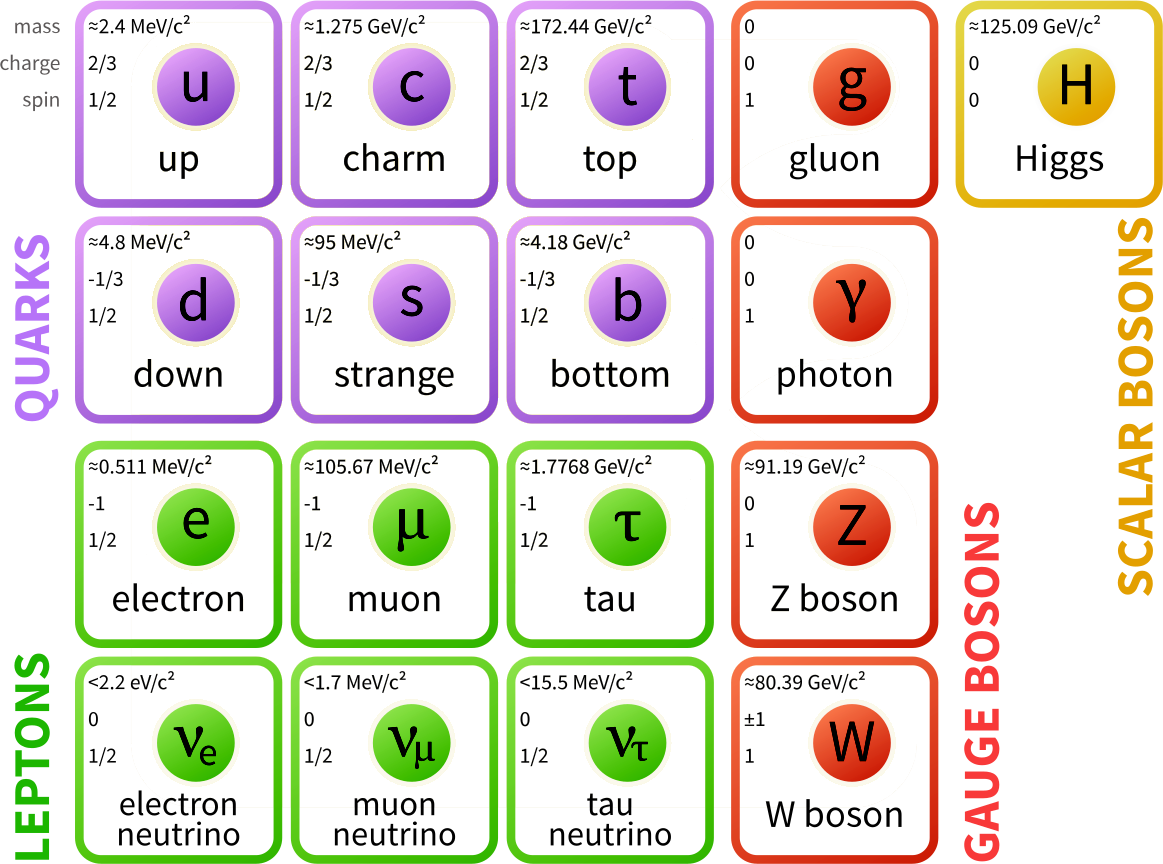
\includegraphics[width=.7\textwidth]{figures/intro/SM-Particles.png}
\caption{\cite{wiki-sm}}
\label{fig:SM-Particles}
\end{figure}

\begin{equation}
\mathcal{L}_{SM} =  - \frac{1}{4} F_{\mu \nu} F^{\mu \nu} + i \bar{\psi} \gamma_\mu D^\mu \psi + \left( y_{ij} \bar{\psi}_i \psi_j + h.c. \right) + |D^\mu \phi|^2 - V (\phi)
\label{eq:sm}
\end{equation}

%I think the

\begin{figure}
\centering
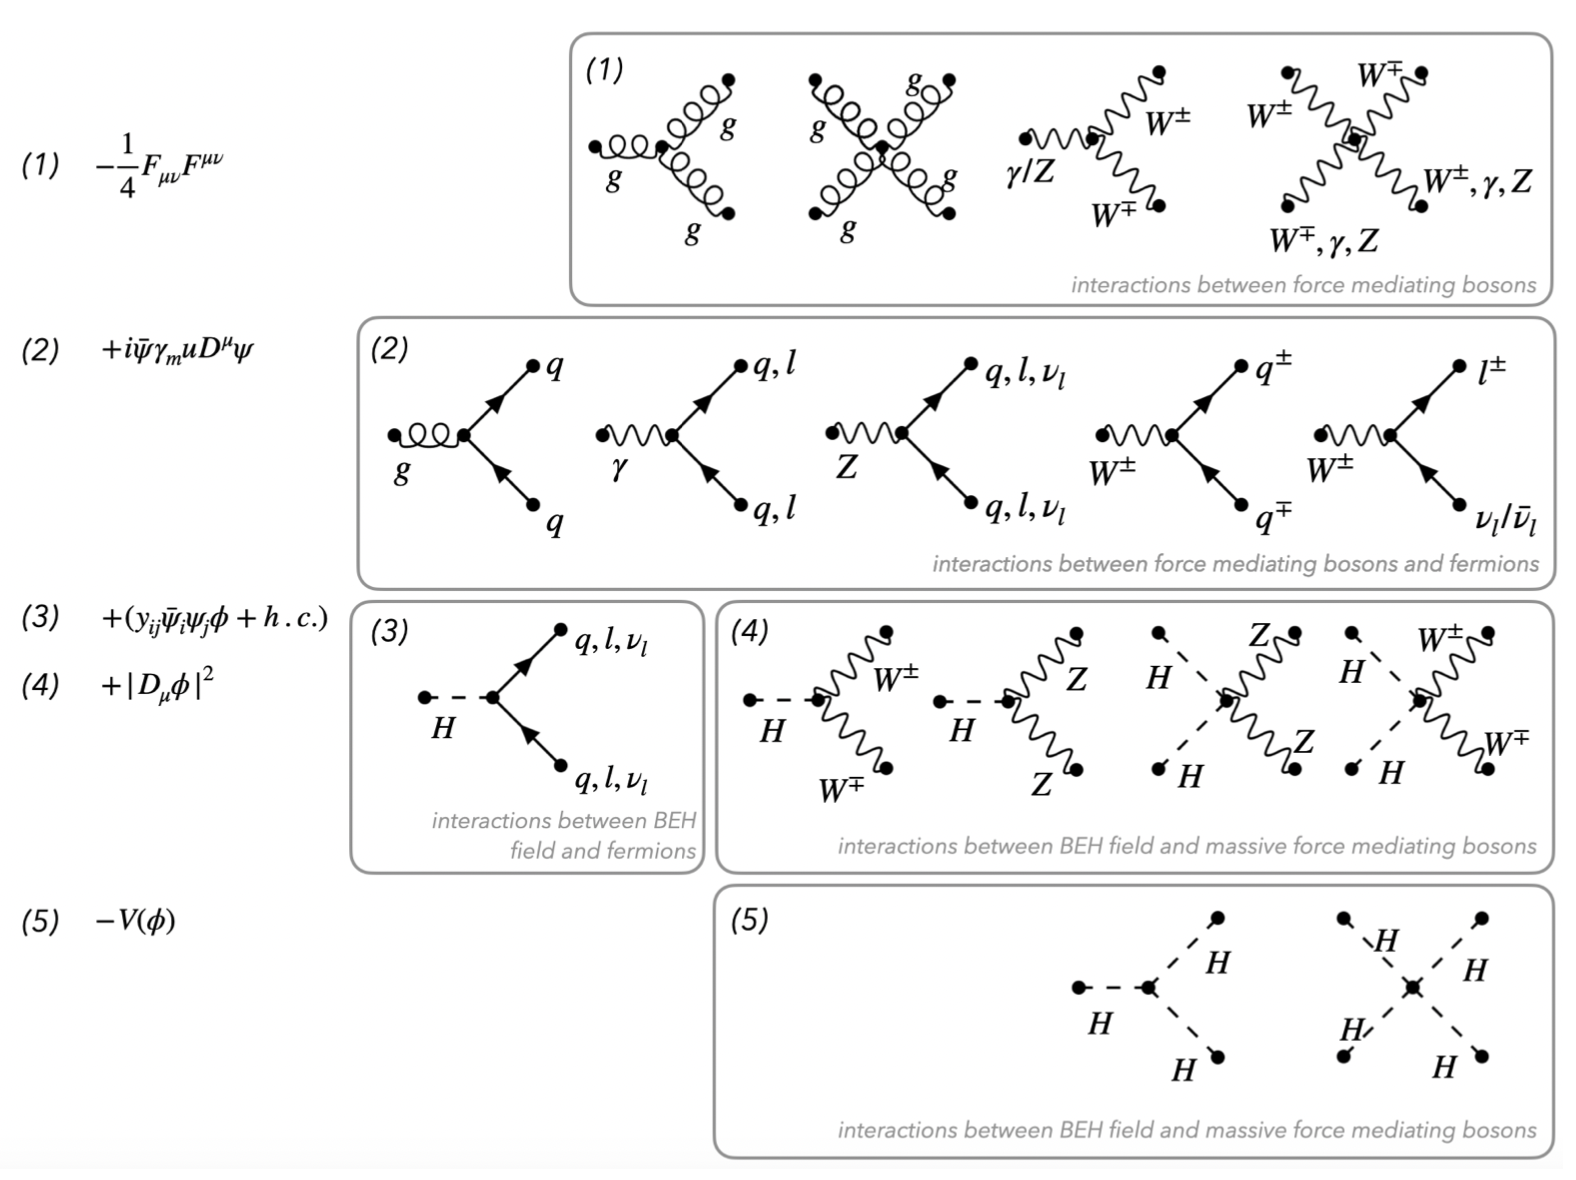
\includegraphics[width=\textwidth]{figures/intro/mel-sm-diagrams.png}
\caption{\cite{Melissa-thesis}}
\label{fig:mel-sm}
\end{figure}

\section{The Higgs mechanism}
I heard from Dale that the pdg is a v good ref for this!!

\section{Effective Field Theories to search for new physics}

\section{Status of the experimental HH results}

\begin{figure}
\centering
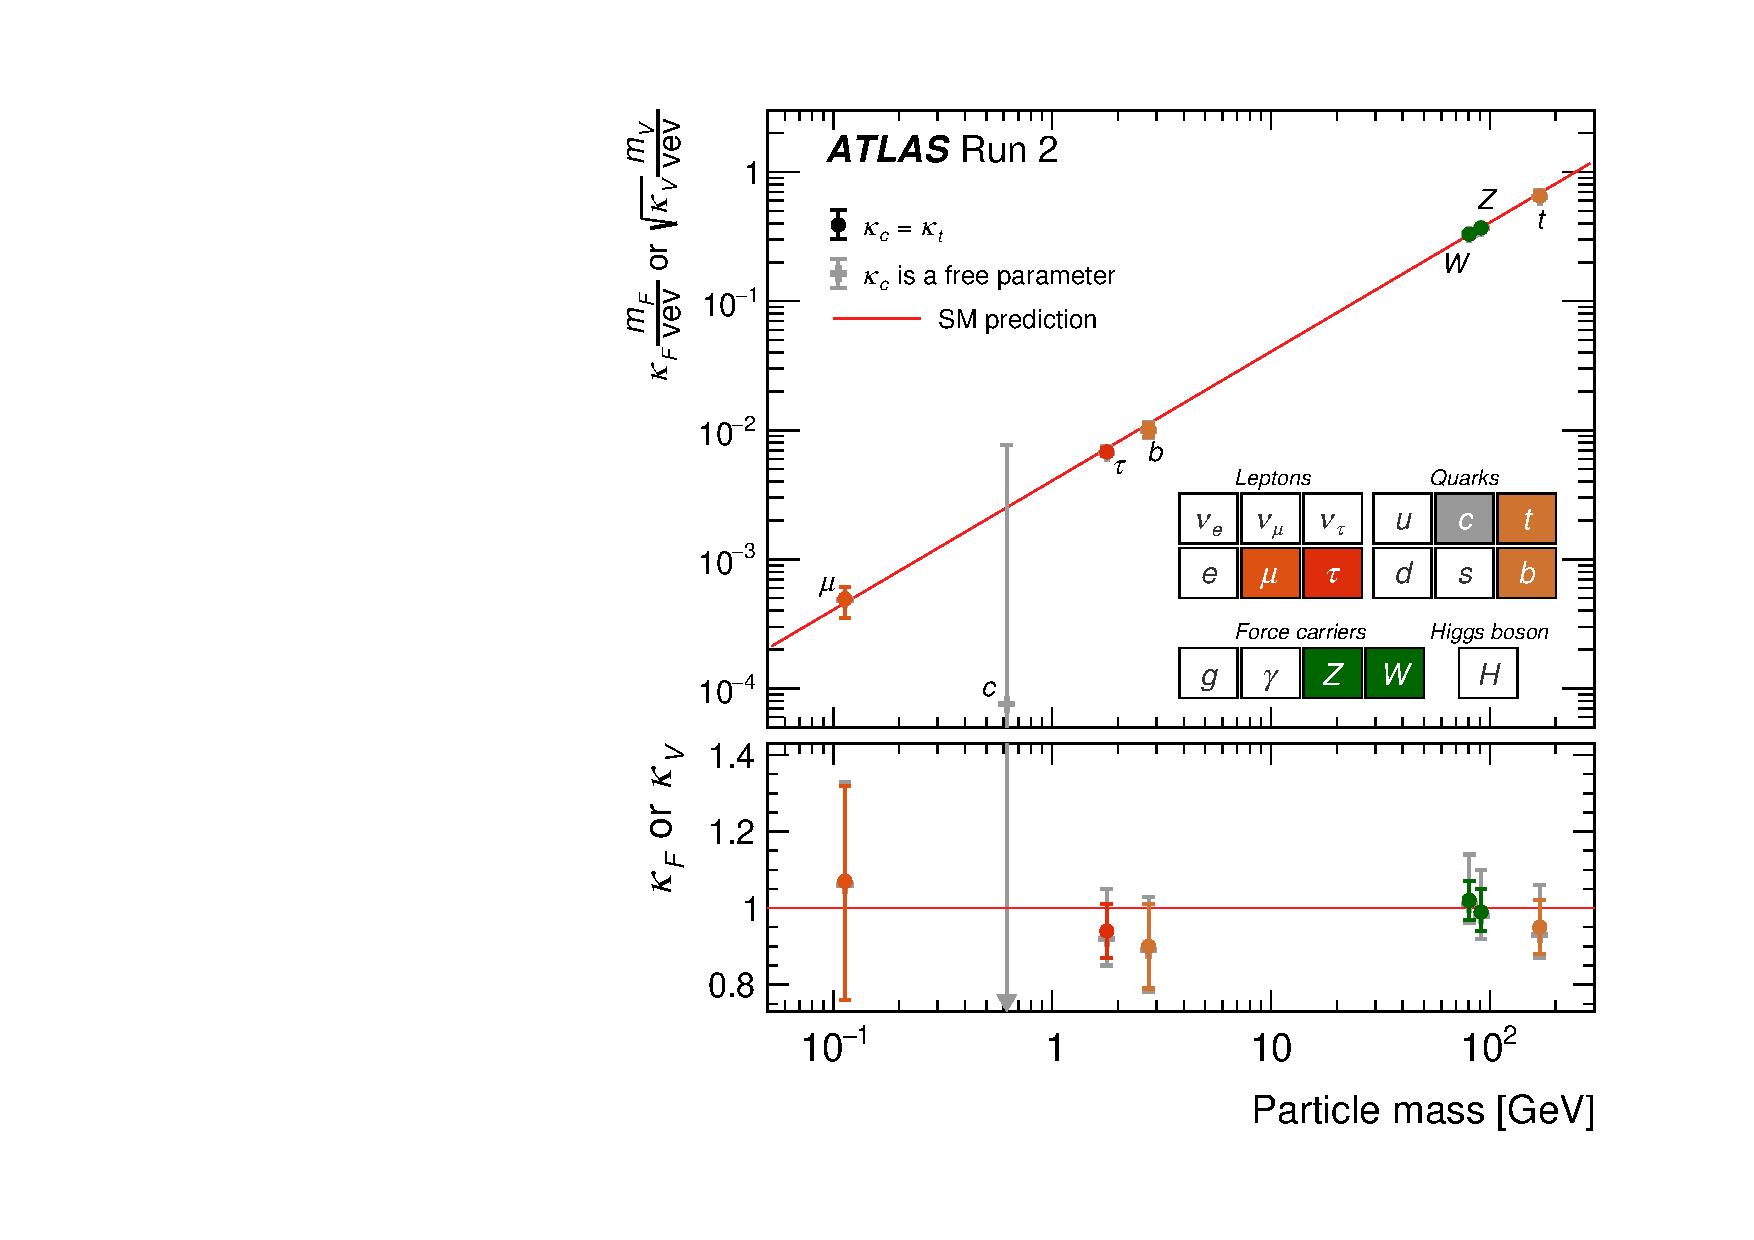
\includegraphics[width=.7\textwidth]{figures/intro/atlas-nature-10yrs/fig_05}
\caption{\cite{2207.00092}}
\label{fig:pcle-mass-atlas}
\end{figure}

\chapter{The Large Hadron Collider}
\label{ch:lhc}
\begin{chapquote}{Pablo Picasso}
{Every act of creation begins with an act of destruction.}
\end{chapquote}


The LHC is a 27~km circumference particle accelerator straddling the border between France and Switzerland \cite{LHC}. It now collides bunches of $10^9$ protons every 25~ns at a center of mass energy of 13~TeV \cite{ATLAS_long}.
Bunches of protons are used since the proton radius is about 1~fm, and thus the probability of a head-on collision between single protons is increased by increasing the number of colliding particles.  We expect about 20 collisions per given bunch crossing at the LHC \cite{PU}.

Since the proton is not an elementary particle, but rather a baryonic resonant QCD bound state, even a head-on collision will not have all of the available energy concentrated at a point.
The proton is a composite particle made up of two up and one down valence quarks, along with a sea of virtual quarks and gluons that spontaneously come out of the vacuum because of the uncertainty relation $\Delta x \Delta p \geq \hbar / 2$.  
The 6.5~TeV per proton is distributed among these partons\footnote[3]{A parton is a constituent of a hadron.}.  Therefore, to look at the high-energy regime, we are interested in a ``hard scatter'' where a single quark or gluon carrying a large fraction of one proton's momentum collides with a high energy constituent of the other proton, lending to the production of one or more Higgs bosons.

\begin{itemize}
	\item History
	\item Collider Stats
	\item I should make a set of slides (or app) making sure that I know what the dipole and focusing magnets do!!
\end{itemize}

\begin{figure}[hbt]
\centering
\subfloat[]{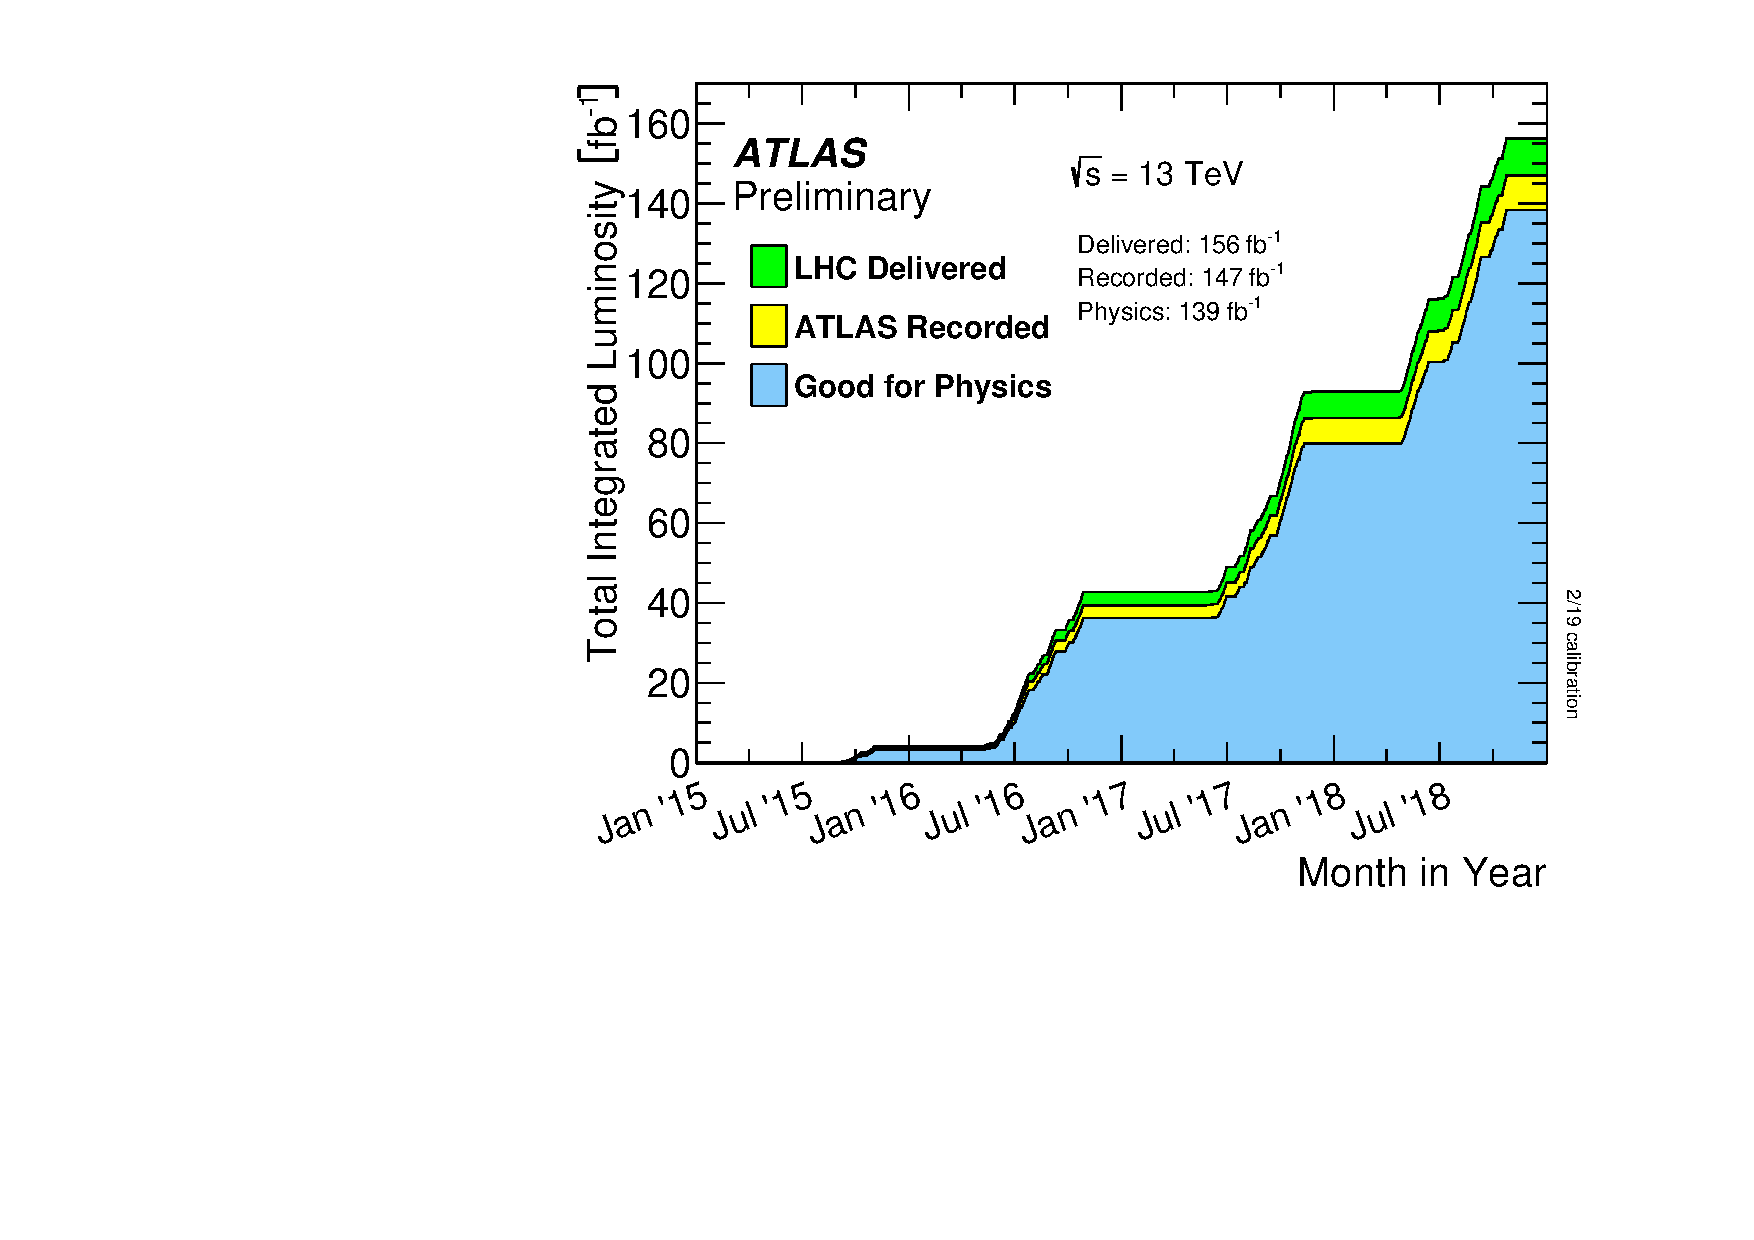
\includegraphics[width=.45\textwidth]{{figures/lhc/intlumivstimeRun2DQall.pdf}}}
\subfloat[]{
	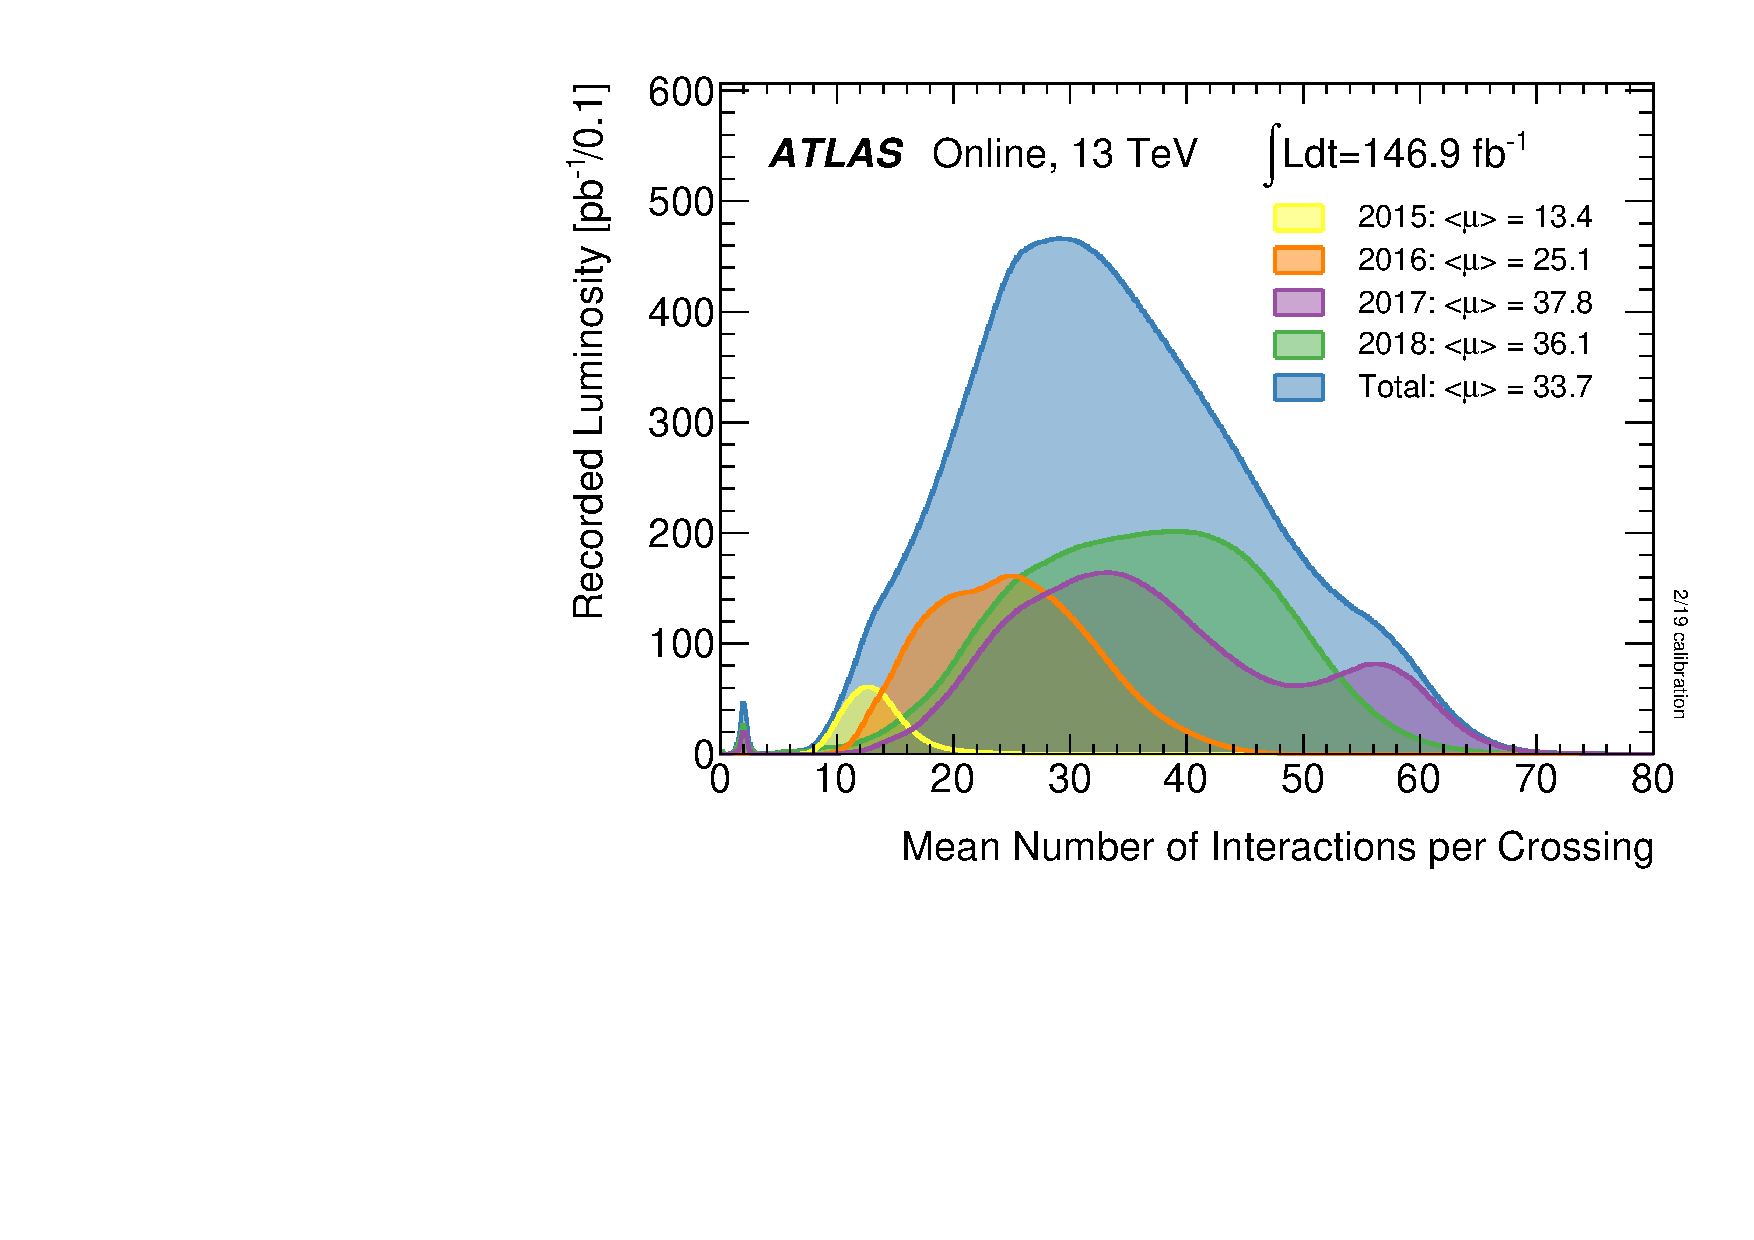
\includegraphics[width=.45\textwidth]{{figures/lhc/mu_2015_2018.pdf}}
	\label{PU density profile for Run~2 data taking.}
	}
\caption{Need to cite: https://twiki.cern.ch/twiki/bin/view/AtlasPublic/LuminosityPublicResultsRun2\#Pileup\_Interactions\_and\_Data\_Tak}
\end{figure}
\chapter{The  ATLAS detector}
\label{ch:atlas}

\section{Tracker}

\section{Calorimeter}

\section{Muon system}

\section{Trigger system}

\hl{Make sure I understand the magnets!!}`

\chapter{Event Reconstruction}
\label{ch:evtReco}

\begin{chapquote}{Hebrews 11:3}
{The things which are seen are not made of the things which do appear.}
\end{chapquote}

The task of event reconstruction involves taking electronic read out signals from the 100 million sensors in the detector and to reconstruct objects that can serve as proxies to the physics observables (i.e, $b$-quarks) % from a HIggs decay)
that to use in high-level physics analysis.
Since the LHC collides protons, %, three quarks held together by gluons
we produce lots of quarks and gluons in the final state, with an example of the signature these particles produce in the detector shown in \Fig{\ref{fig:tracks-clusters-annotated}}.

\begin{figure}[hbt]
\centering
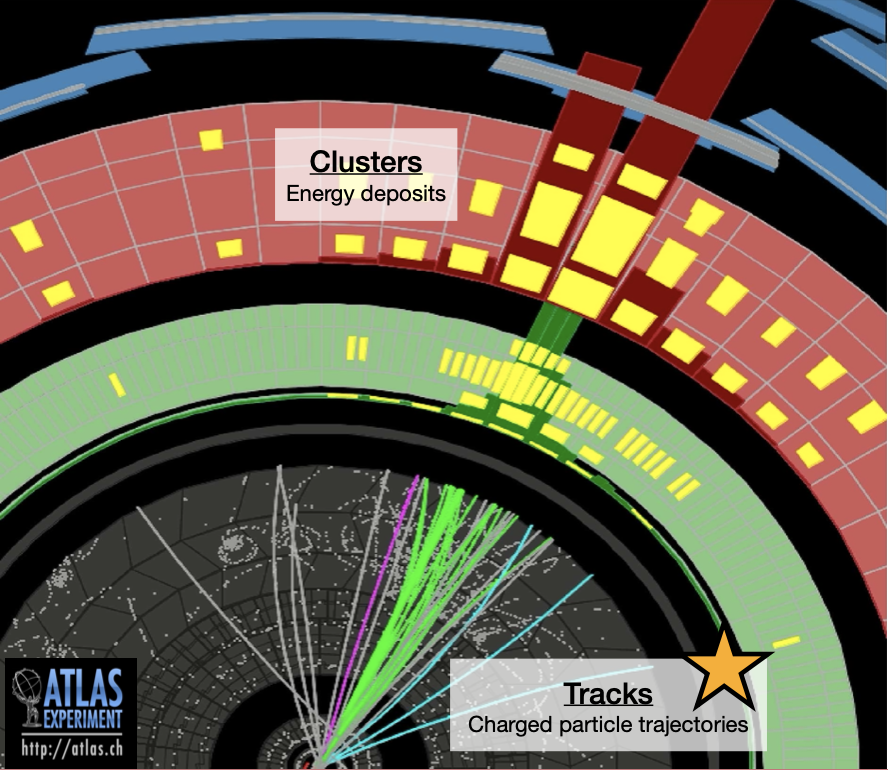
\includegraphics[width=.6\textwidth]{figures/cp-graphics/tracks-clusters-annotated}
\caption{Illustration of what a jet looks like in our detector}
\label{fig:tracks-clusters-annotated}
\end{figure}

Since this thesis deals with an analysis with an all-hadronic final states, these are the key input objects for the analysis and for my work in \Pqb-tagging, so in this chapter we focus on the reconstruction of these types of events.
We include this graphic here, because it nicely demonstrates the outline for this chapter
The charged particle trajectories in the inner detector form a set of tracks, and will be described in \Sect{\ref{sec:tracks}}.
The tracks that originate from the same location are then reconstructed into vertices, as described in \Sect{\ref{sec:vertices}}.
The unsupervised learning algorithms that get reconstructs the quark and gluon decay products into the ``jets'' are described in \Sect{\ref{sec:jets}}.
Finally, we conclude with the reconstruction muon tracks in \Sect{\ref{sec:muons}}.


\textbf{Citation:} The European Physical Journal C Vol 73 3 (2013) 2304
% Note - if I include this, I \emph{know} that Pat will ask me about the details, so I should make sure I understand the color coding, etc.

\section{Tracks}
\label{sec:tracks}

\subsection{Track reconstruction}

To cite: \cite{soft-pub-2007-007}

\textbf{Inside out:}
\begin{itemize}
	\item Cluster formation
	\item Seed finding: reco triplets of hits from the pixel detector
	\item Track fitting with a combinatorial Kalman filter
	\item Ambiguity solving of which hits with a collection of NNs which decides whether a given cluster is shared between two tracks and how to split the energy depostion between these multiple tracks \cite{jinst-9-2014-P09009}
	\item Extend to the TRT hits
\end{itemize}

Improve the efficiency due to tracks in that have decays displaced from the original collision point with an \textbf{outside in:} track reconstruction alrogihm
\begin{itemize}
	\item Start with the seeds from the TRT
	\item Extend to the hits in the silicon detector
	\item Again use an ambiguity solver.
\end{itemize}

\begin{figure}[hbt]
\centering
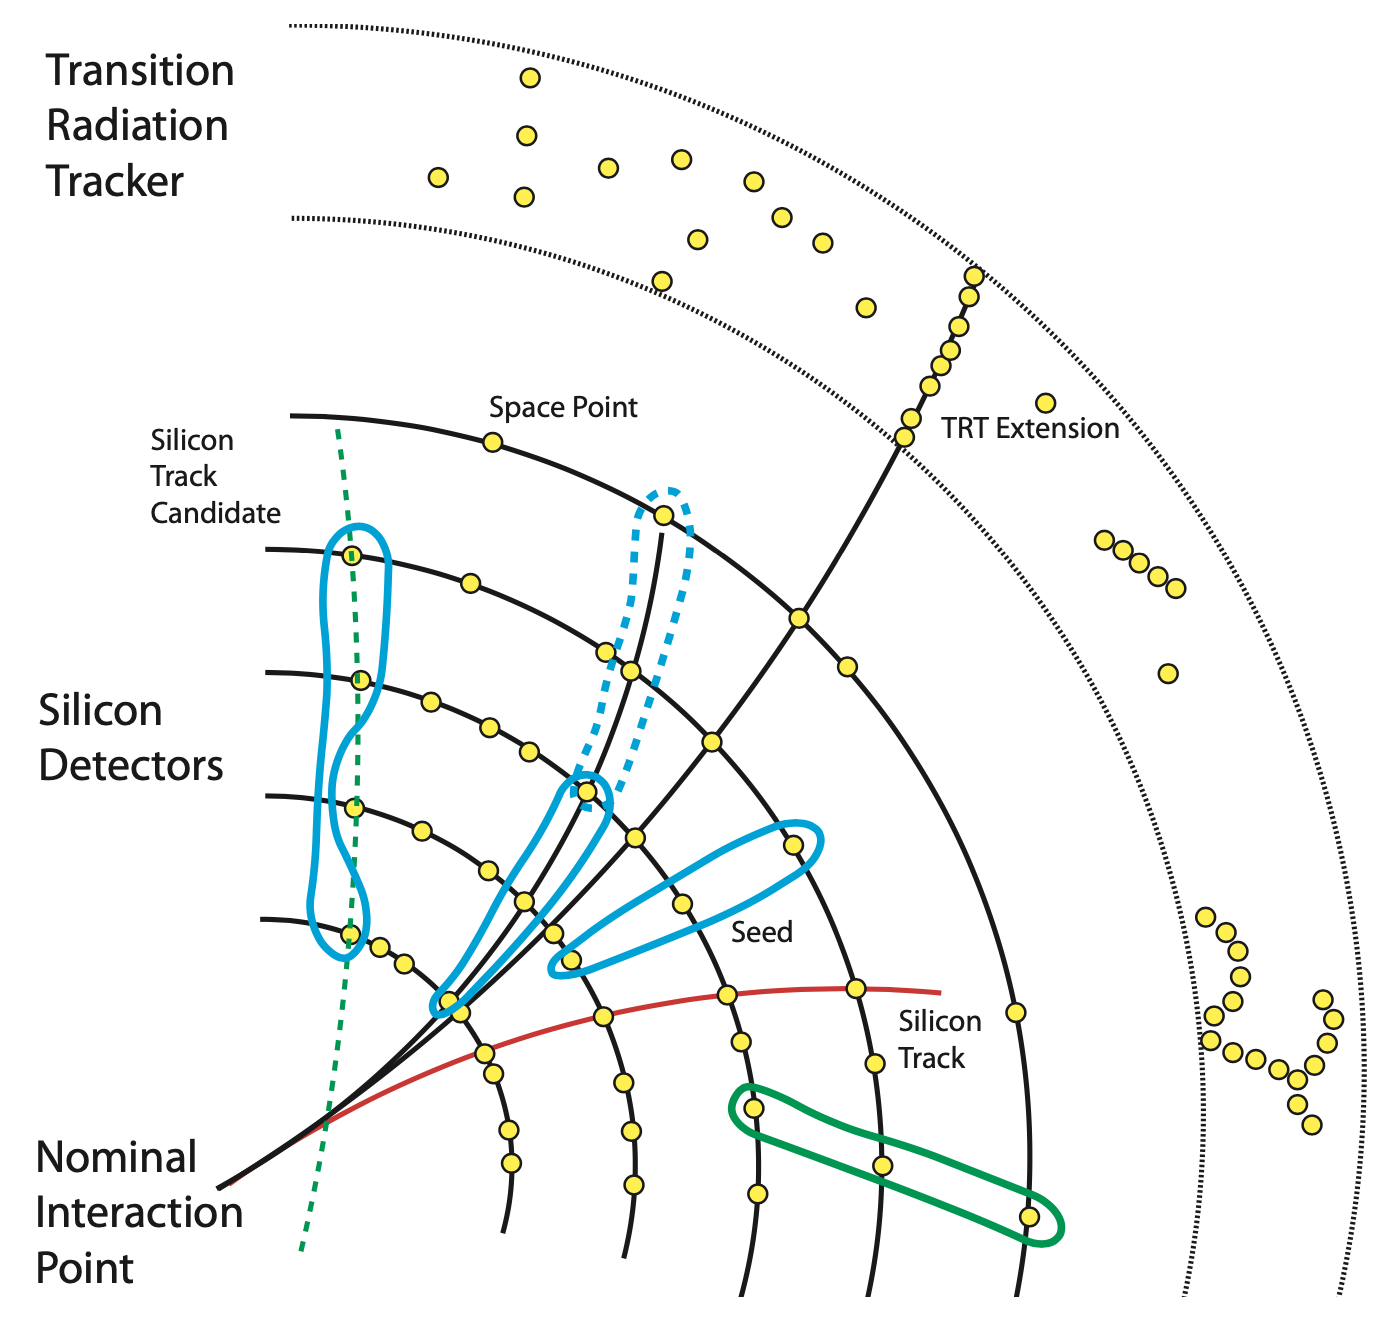
\includegraphics[width=0.6\textwidth]{figures/cp-graphics/tracking/track-reco}
\caption{\hl{need to ask Valentina where this pic was from originally}.}
\label{fig:track-reco}
\end{figure}


\subsection{Challenges in Dense Environments}

\begin{figure}[hbt]
\centering
\subfloat[]{
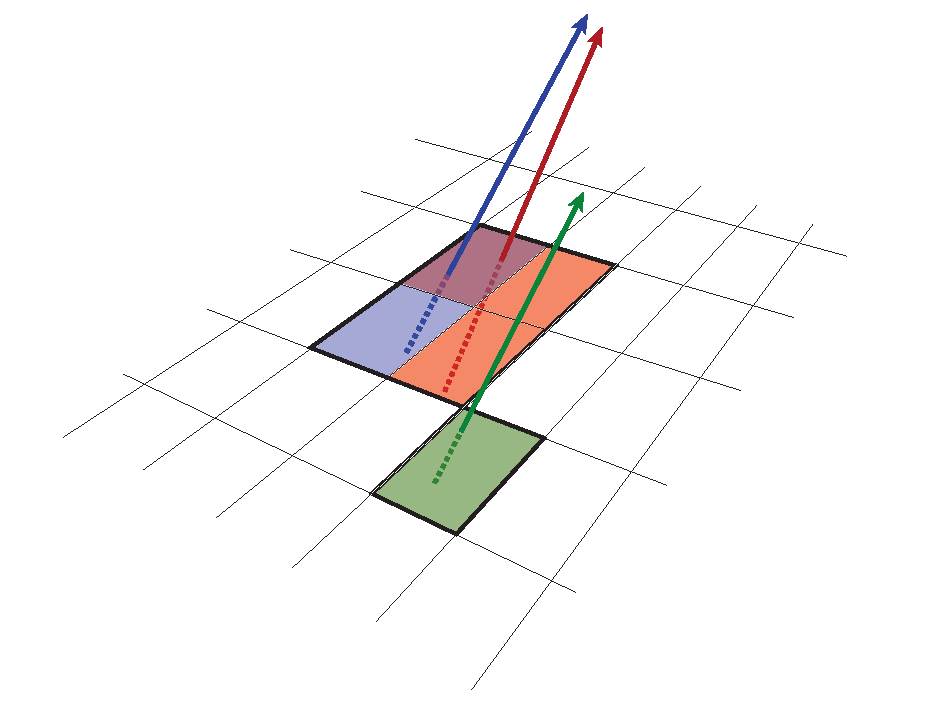
\includegraphics[width=0.43\textwidth]{figures/cp-graphics/jinst-9-2014-P09009/fig_03}
}
\subfloat[]{
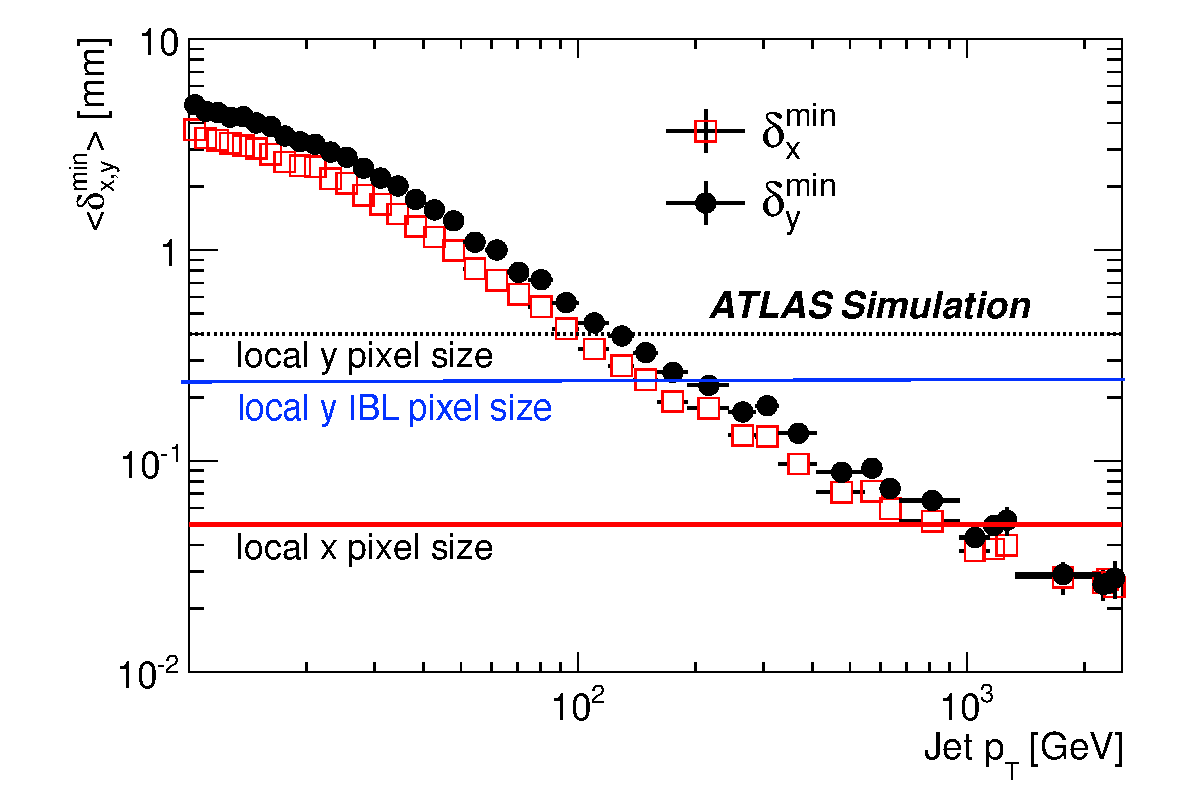
\includegraphics[width=0.55\textwidth]{figures/cp-graphics/jinst-9-2014-P09009/fig_04}
}
\caption{\cite{jinst-9-2014-P09009}.}
\label{fig:ctide}
\end{figure}


\subsection{Discussion of inputs}


\begin{figure}[hbt]
\centering
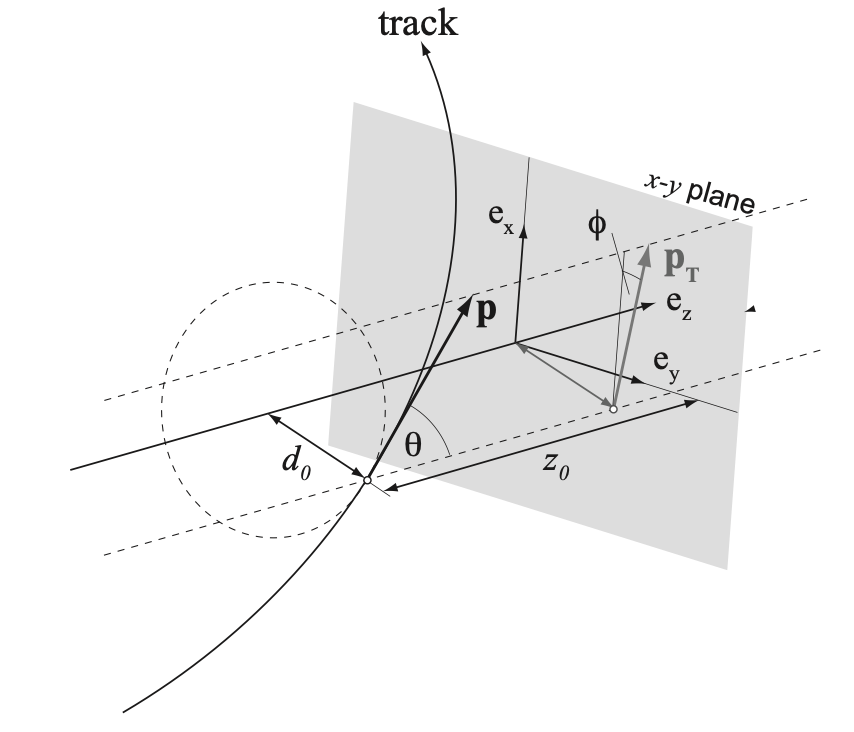
\includegraphics[width=0.6\textwidth]{figures/cp-graphics/ATL-SOFT-PUB-2007-003/fig-2a}
\caption{\cite{ATL-SOFT-PUB-2007-003}}
\label{fig:ATL-SOFT-PUB-2007-003-fig-2a}
\end{figure}

\begin{figure}[hbt]
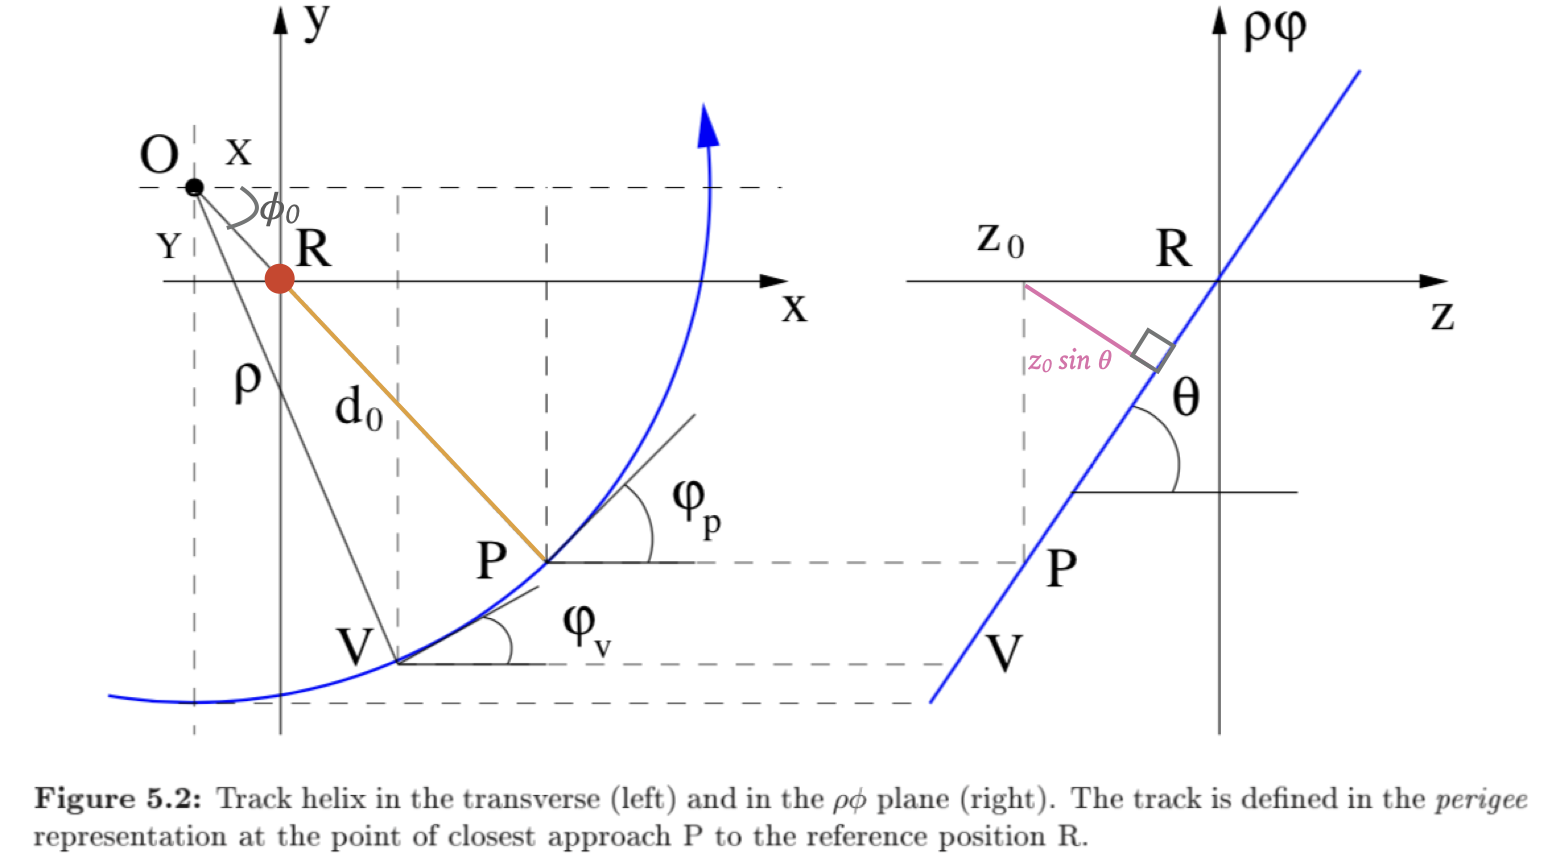
\includegraphics[width=\textwidth]{figures/cp-graphics/giacinto-fig-5.2}
\caption{\cite{giacinto-thesis}}
\label{fig:track-2d-graphics}
\end{figure}

\begin{itemize}
	\item \textcolor{red}{R}: reference position at which the tracks are defined, i.e, for \Pqb-tagging we use the primary vertex of the collision as the reference point. 
	\item \textcolor{orange}{$d_0$}:  The transverse impact parameter, point of closest approach (POCA) in the transverse plane with respect to R.
	\item \textcolor{pink}{$z_0 \sin \theta$}:  The longitudinal impact parameter, or the longitudinal displacement from the POCA (defined in the transverse plane). The multiplication by $\sin \theta$ term is included because it characterizes the 2d distance from $z_0$ to the closest point along the track trajectory.
\end{itemize}


\begin{align}
x_V &= x_R + d_0 \cos \left( \phi_p + \frac{\pi}{2} \right)+ \rho \left[  \cos \left( \phi_V + \frac{\pi}{2}  -  \cos \left( \phi_p + \frac{\pi}{2} \right)\right)  \right] \notag \\
y_V &= y_R + d_0 \sin \left( \phi_p + \frac{\pi}{2} \right)+ \rho \left[  \sin \left( \phi_V + \frac{\pi}{2}  -  \sin \left( \phi_p + \frac{\pi}{2} \right)\right)  \right] \\
z_V &= z_R + z_0 - \frac{\rho}{\tan \left( \theta \right) } \left[ \phi_V - \phi_p \right] \notag
\end{align}

\begin{figure}[hbt]
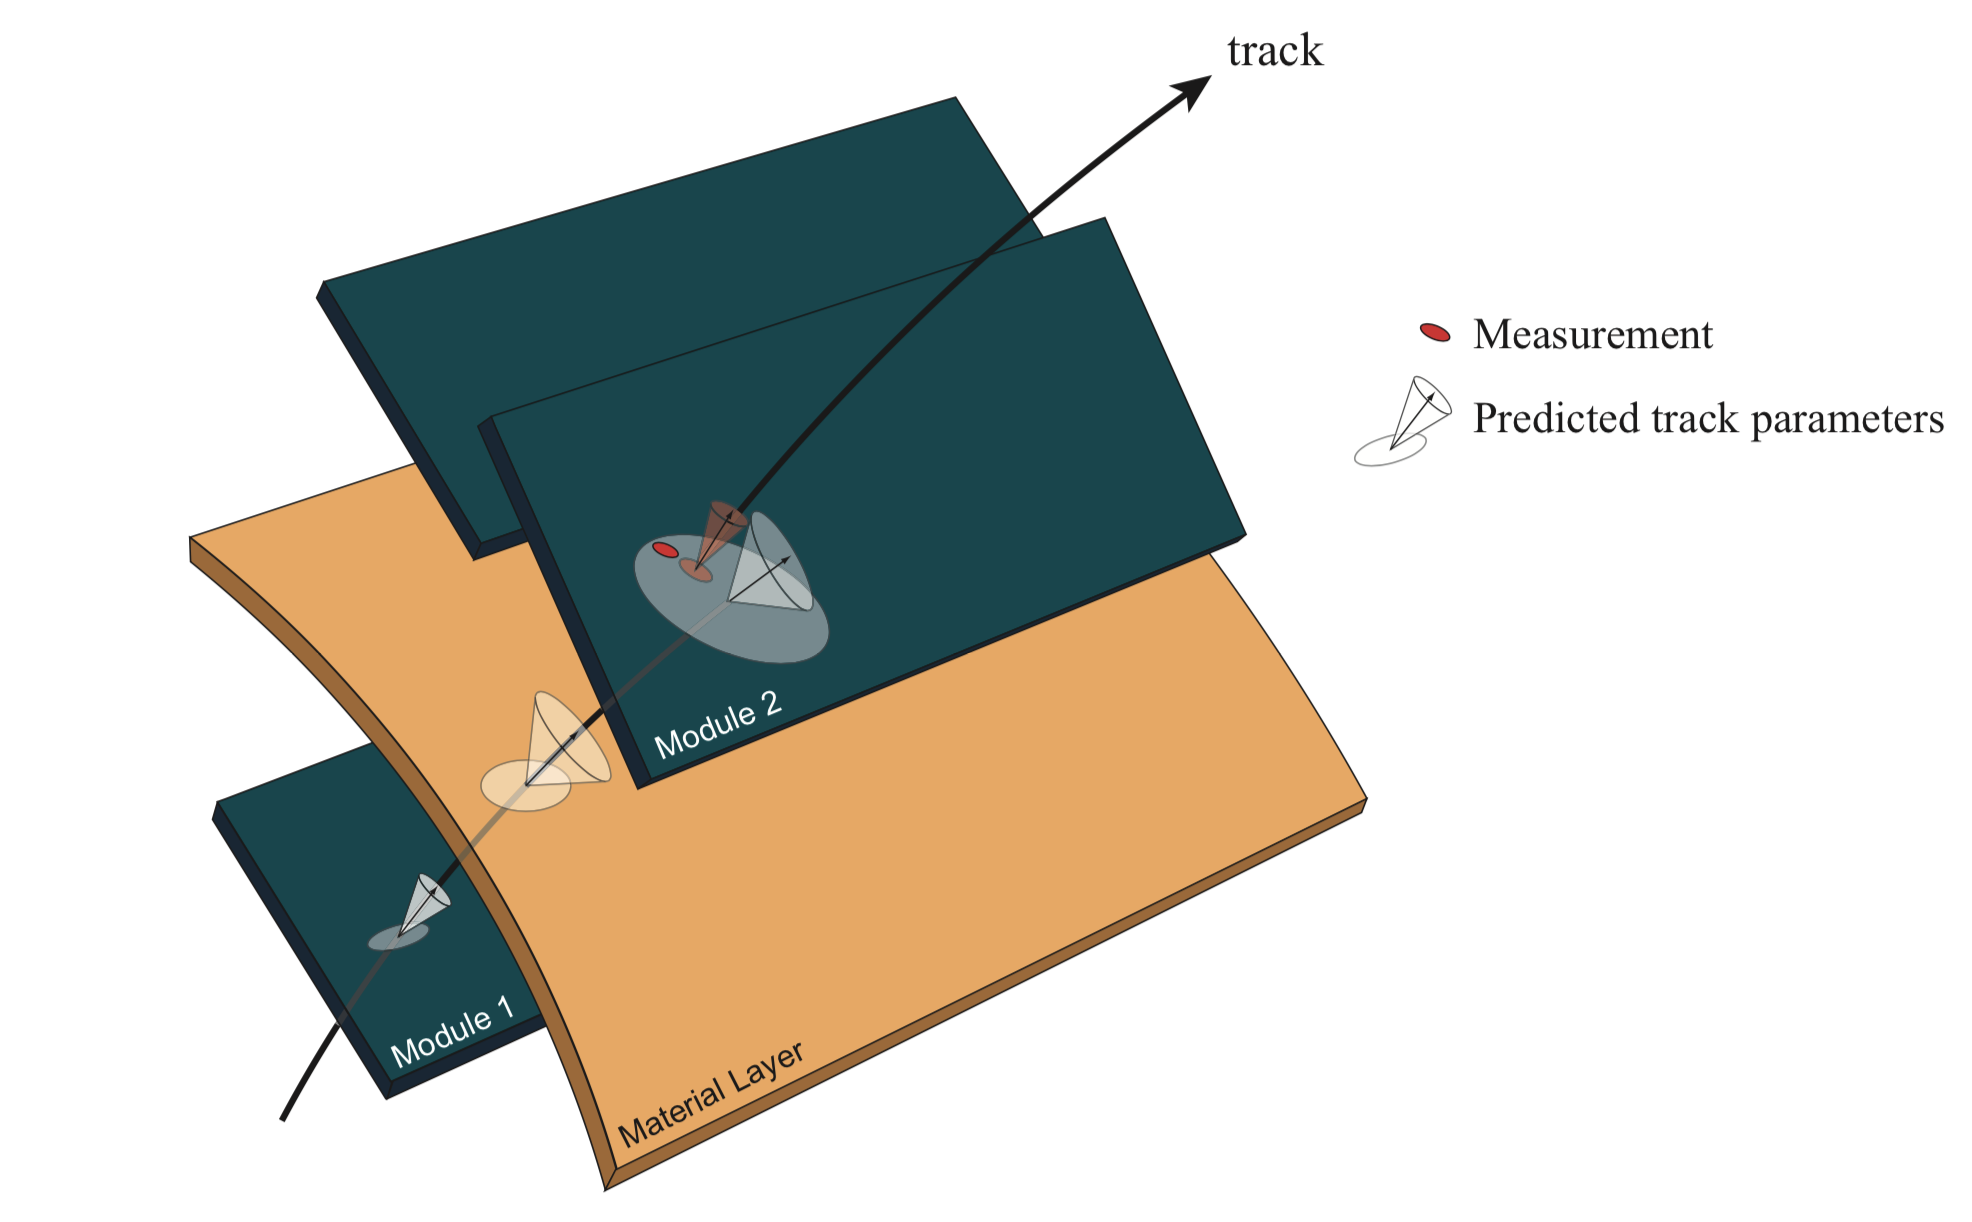
\includegraphics[width=\textwidth]{figures/cp-graphics/ATL-SOFT-PUB-2007-005/track-extrap-material-int}
\caption{Visualization of the track extrapolation with its associated errors \cite{ATL-SOFT-PUB-2007-005}.}
\label{fig:track-extrap-material-int}
\end{figure}

\begin{equation}
\rho = \frac{\sin \theta}{\frac{q}{p} B_z}
\end{equation}

\begin{align}
d_0 &= \text{sign} \left( d_0 - \rho \right) \sqrt{\left(x_V - x_R - \rho \cos \left(\phi_V + \frac{\pi}{2} \right) \right)^2 +  \left(y_V - y_R - \rho \sin \left(\phi_V + \frac{\pi}{2} \right) \right)^2 } \\
\phi_p &= \arctan \left( \frac{y_V - y_R - \rho \sin \left( \phi_V + \frac{\pi}{2}\right)}{x_V - x_R - \rho \cos \left( \phi_V + \frac{\pi}{2}\right)} \right) \\
z_0 &= z_R + z_V + \frac{\rho}{\tan \theta } \left[ \phi_V - \phi_p (x_V, y_V, z_V, \theta, q/p) \right]\\
\left( \frac{q}{p} \right)_P &= \left( \frac{q}{p} \right)_V \\
\theta_P &= \theta_V
\end{align}

The way we map from one representation to another is by calculating the Jacobians of the transformations:

\begin{equation}
A = \frac{\partial (d_0, z_0, \phi_P, \theta_P, q/p)}{\partial (x_V, y_V, z_V)} = 
\begin{bmatrix}
- h \frac{X}{S} & - h \frac{Y}{S} & 0 \\
\frac{\rho}{\tan \theta}  \frac{Y}{S^2} & - \frac{\rho}{\tan \theta}  \frac{X}{S^2}  & 1 \\
- \frac{Y}{S^2} &  \frac{X}{S^2} & 0 \\
0 & 0 & 0 \\
0 & 0 & 0
\end{bmatrix}
\end{equation}

\begin{equation}
B =  \frac{\partial (d_0, z_0, \phi_P, \theta_P, q/p)}{\partial (\phi_V, \theta, q/p)} = 
\begin{bmatrix}
- \frac{h \rho}{S} R & \frac{\rho}{\tan \theta} \left[ 1 - \frac{h}{S} R \right]  & - \frac{\rho}{q/p} \left[ \Delta \phi - \frac{h}{S} R  \right]  \\
\frac{\rho}{\tan \theta}  \left[ 1 - \frac{\rho}{S^2} Q \right] & \rho \left[ \Delta \phi + \frac{\rho}{S^2 \tan^2 \theta } R \right] & \frac{\rho}{q/p \tan \theta}\left[ \Delta \phi - \frac{\rho}{S^2} R \right] \\
\frac{\rho}{S^2} Q & - \frac{\rho}{S^2 \tan \theta}   R & \frac{\rho}{S^2 q/p}   R \\
0 & 1 & 0 \\
0 & 0 & 1 
\end{bmatrix}
\end{equation}


where:
\begin{align*}
X &= x_V - x_R - \rho \cos \left(\phi_V + \frac{\pi}{2} \right) 
Y &= y_V - y_R - \rho \sin \left( \phi_V + \frac{\pi}{2}\right)
R &= Y \sin \phi_V + X \cos \phi_V \\
Q &= X \sin \phi_V - Y \cos \phi_V \\
S &= \sqrt{X^2 + Y^2} \\
h &= \text{sign}  \rho \\
\phi &= \phi_P - \phi_V
\end{align*}

\textbf{Q:} How do we define the sign of $\rho$?

\subsection{The perigee parameters}

\FloatBarrier
\clearpage
\section{Vertexing}
\label{sec:vertexing}

\subsection{General problem formulation}

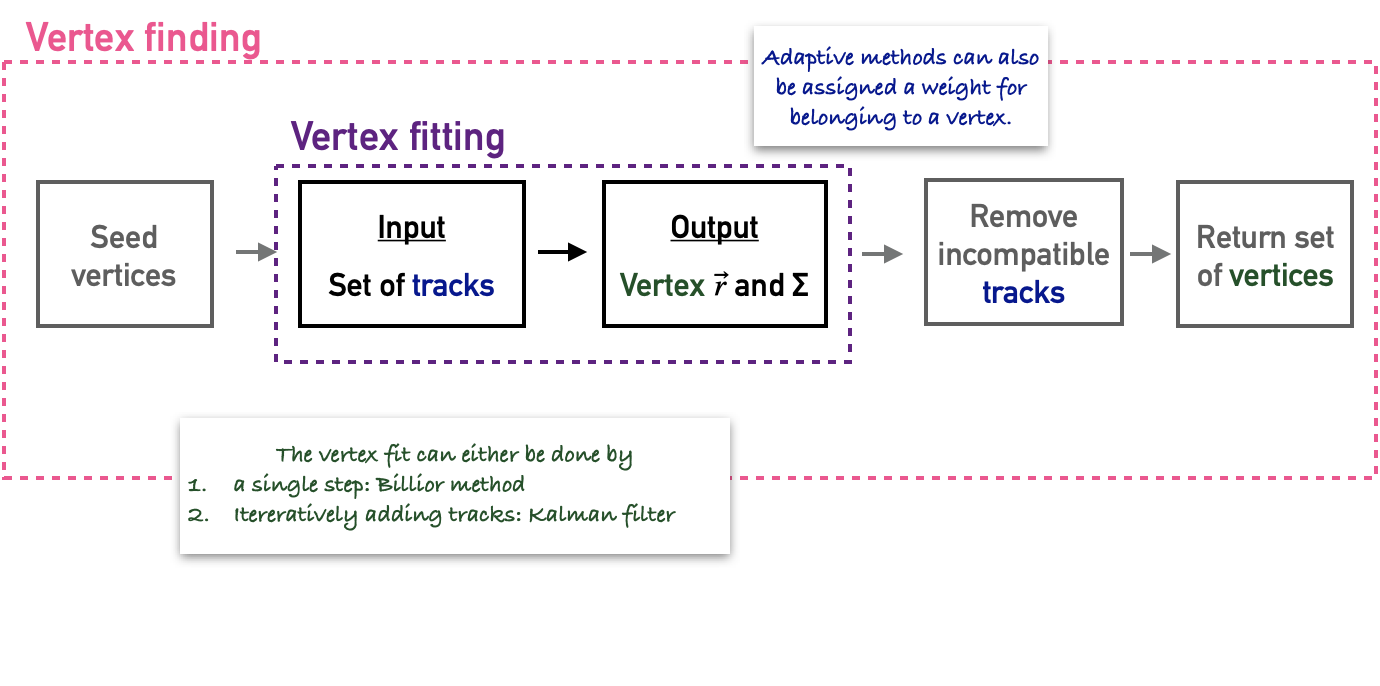
\includegraphics[width=\textwidth]{figures/cp-graphics/Vertex-finding-fitting}

The \textcolor{rebeccapurple}{Vertex fit:} Position which maximizes the likelihood for the probability density tubes for the tracks to all intersect at this point \cite{giacinto-thesis}. 
This is seen mathematically by \Eq{\ref{eq:vtx-prob-density-fct}} below, where $\vec{r}$ is the position of the vertex, and $\vec{r}_i(\phi_{p,i})$ is track $i$ and $\phi_{p,i}$ parametrizes what point of the trajectory that we're on.

\begin{equation}
P(\vec{r}) = \int d \phi_{p,1} d \phi_{p,2} \ldots d \phi_{p,n} \prod_{i=1}^{n_{trk}} 
\exp \left[ - \frac{1}{2}  \left(\vec{r} - \vec{r}_i (\phi_{i,i})\right)^T COV^{-1}_{3x3} (\phi_{p,i}) \left(\vec{r} - \vec{r}_i (\phi_{i,i})\right) \right]
\label{eq:vtx-prob-density-fct}
\end{equation}

\hl{Is this cov matrix the vertex cov? If so, should I call it $\Sigma$ instead of $Cov_{3x3}$?}

\subsection{Primary vertex reconstruction}

The event's selected primary vertex (PV) is defined as the reconstructed primary vertex with largest $\sum \pT^2$ of the associated tracks. 


\clearpage
\section{Jets}

\subsection{Jet clustering algorithms}

A given $pp$ collision produces many quarks and gluons.  However, because of the ``confinement principle,'' no free color charge can exist, which means no isolated quarks or gluons can exist in nature. %\cite{SM_Higgs, Particle_World}.  
It becomes energetically favorable for quark / anti-quark pairs to pop out of the vacuum to balance the color charge imbalance by forming color neutral hadrons. 
This sparks a chain reaction which produces a spray of particles in the detector. 

The anti-k$_T$ algorithm provides a way to cluster the energy deposited in the calorimeter to form a ``jet,'' and is the standard algorithm for defining jets at ATLAS \cite{antiKt}.  First it defines two quantities, 
%
\begin{equation}
d_{ij} = {\text{min}}( p_{Ti}^{-2}, p_{Tj}^{-2}) \frac{\Delta R_{ij}}{R^2} \qquad \qquad  d_i = p_{Ti}^{-2}
\end{equation}
%
where $\Delta R_{ij}^2 = (y_i - y_j)^2 + (\phi_i - \phi_j)^2$, and $R$ is the jet-radius, defined by the user.  To find the jets, the algorithm
%
\begin{itemize}
\item{Calculates $d_{ij}$ and $d_i$ for all particles in the event, and lets $d$ be the smallest $d_i$, $d_{ij}$.}
%\item{Find all the $d_{ij}$ and $d_i$ in the event, and let $d = min(\{d_{ij}, D_i\})$}
	\begin{itemize}
	\item{If $d = d_{ij}$, then it combines jet $i$ and jet $j$.}
	\item{If $d = d_{i}$, then it lets jet $i$ be the final jet.}
	\end{itemize}
\item{It continues the previous steps until all the particles in the event have been accounted for.}
\end{itemize}
%
This algorithm clusters high-$p_T$ particles together if they fall within the jet's radius. \\

The $pp$ collisions at 13~TeV typically will give rise to about 20 moderate $p_T$ jets in the detector, or around ${{20}\choose{2}} = 190$ viable di-jet candates.  So the challenge in elucidating the $H\rightarrow b\bar{b}$ or $HH \rightarrow 4b$ signals is accurately finding the ``correct'' pair(s) of jets.

Since the protons are not point-like, the colliding partons may not have equal $p_T$ in the lab frame. By definition, the net momentum will be zero in the center of mass (CM) frame.  A heavy ($\sim$TeV) resonance can be created at (or nearly at) rest in the CM frame, but when Lorentz boosting back into the lab frame the decay products can become highly collimated.  When the decay products can no longer be resolved individually, we instead search for jets with a large radius parameter (``fat jets''), indicative of merged jets \cite{SM_Higgs, Merged_Jets}.  The constituent clusters inside a fat jet are called \emph{subjets}.  
Large R (about 1.0) correspond to fat jets, and R about 0.4 correspond to the standard resolved jets.

\subsection{PFlow}

\emph{Why better?}

\textbf{To cite for pT plot:}
2007.02645 \\
Eur. Phys. J. C 81 (2021) 689

\textbf{To cite for $\phi$ plot:}
https://indico.cern.ch/event/777980/contributions/3236356/subcontributions/271401/attachments/1780062/2896765/JESJER.pdf

\begin{figure}
\centering
\subfloat[\pt resolution]{
	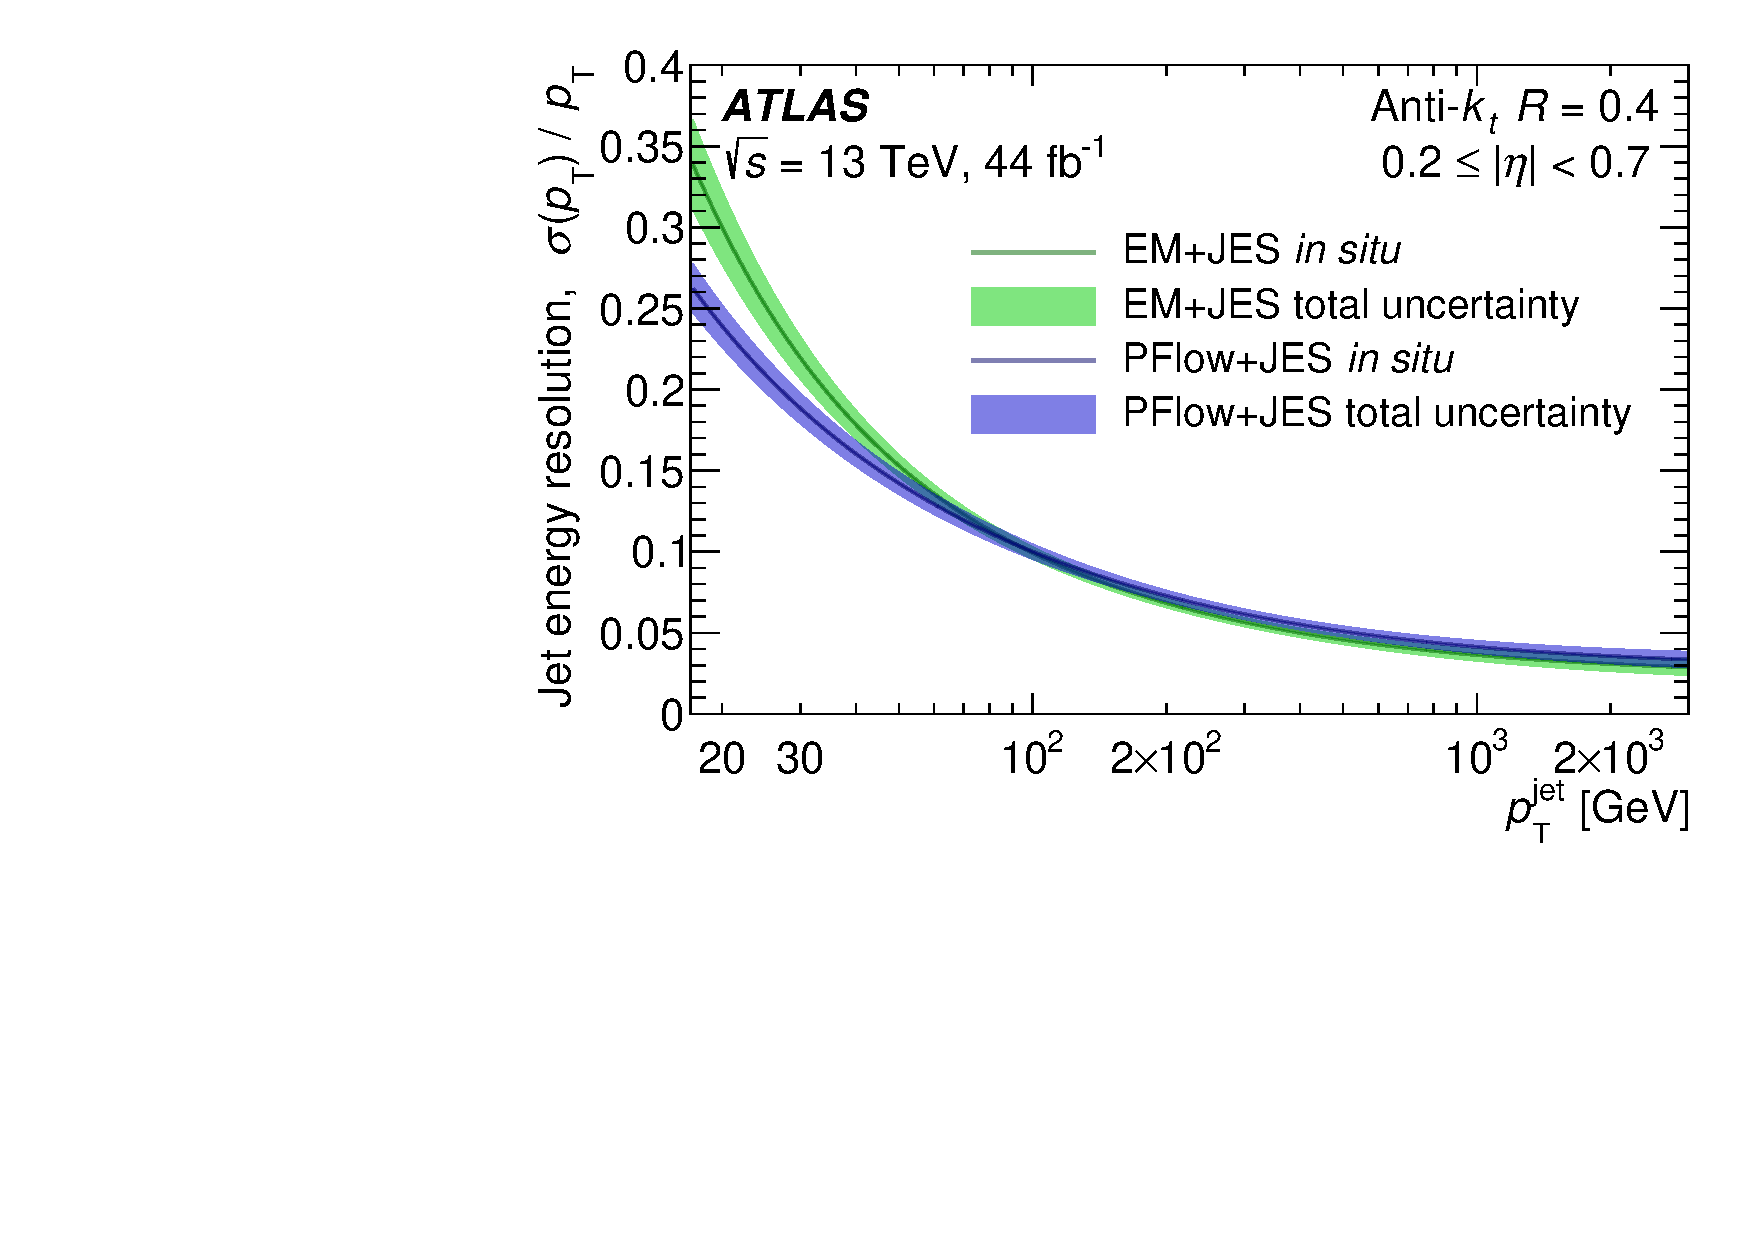
\includegraphics[height=5.4cm]{{figures/cp-graphics/jets/fig_30a}}
	\label{fig:jet-pflow-pt-res}
	}
\subfloat[$\phi$ resolution]{
	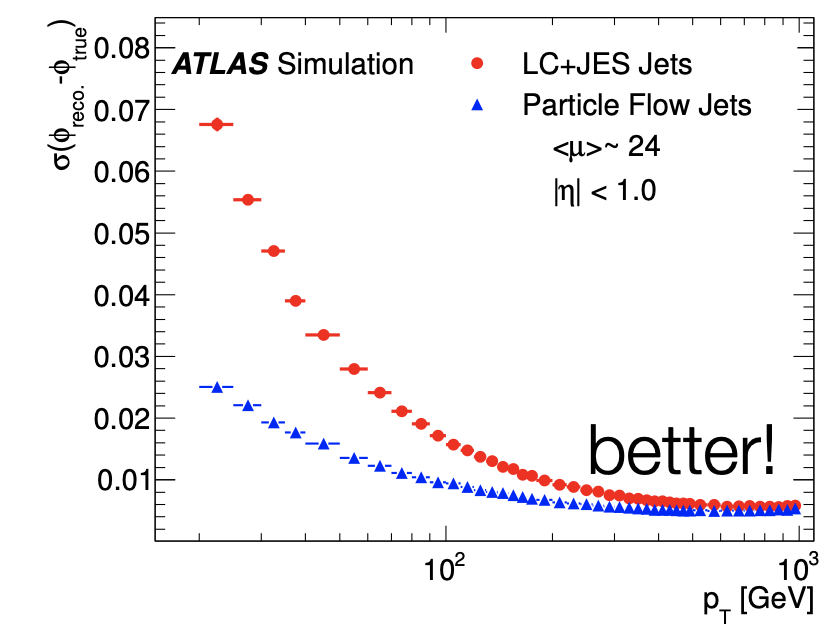
\includegraphics[height=5.4cm]{{figures/cp-graphics/jets/phi_reco}}
	\label{fig:jet-pflow-phi-res}
	}
\caption{Improvement for moving to the PFlow algorithm for jet reconstruction.}
\end{figure}

\subsection{Boosted jets}

\subsection{VR track jets}


\section{Muons}
\label{sec:muons}

Def useful for muon in jet + pt reco correction!!
%Also - for describing the DL1rmu tagger .

%\subsection{Pileup suppression}
%\subsection{Event cleaning}
% I'm tempted to talk about these, but since they're not directly related 
% to the core contributions of my thesis work, I'm going to skip it.
% Oh - I should j add what I put in the int note!!


\chapter{b-tagging}
\begin{chapquote}{Michael Nielson, \emph{Neural Networks and Deep Learning}}{Technical expertise is the mastery of complexity -- creativity is the mastery of simplicity.}
\end{chapquote}

\section{Introduction}
\label{sec:ftag-intro}

For the physics program of the ATLAS experiment at the Large Hadron Collider (LHC), the identification of jets initiated by $b$-quarks, or $b$-tagging, is a fundamental tool. 
Ensuring its optimal performance is particularly important for the study of the Higgs boson and the top quark \cite{HIGG-2018-04, HIGG-2018-13}, as well as many exotic extensions of the Standard Model with resonances preferentially decaying to heavy quarks \cite{ATLASdijetres}. 


\begin{figure}[htbp]
  \centering
  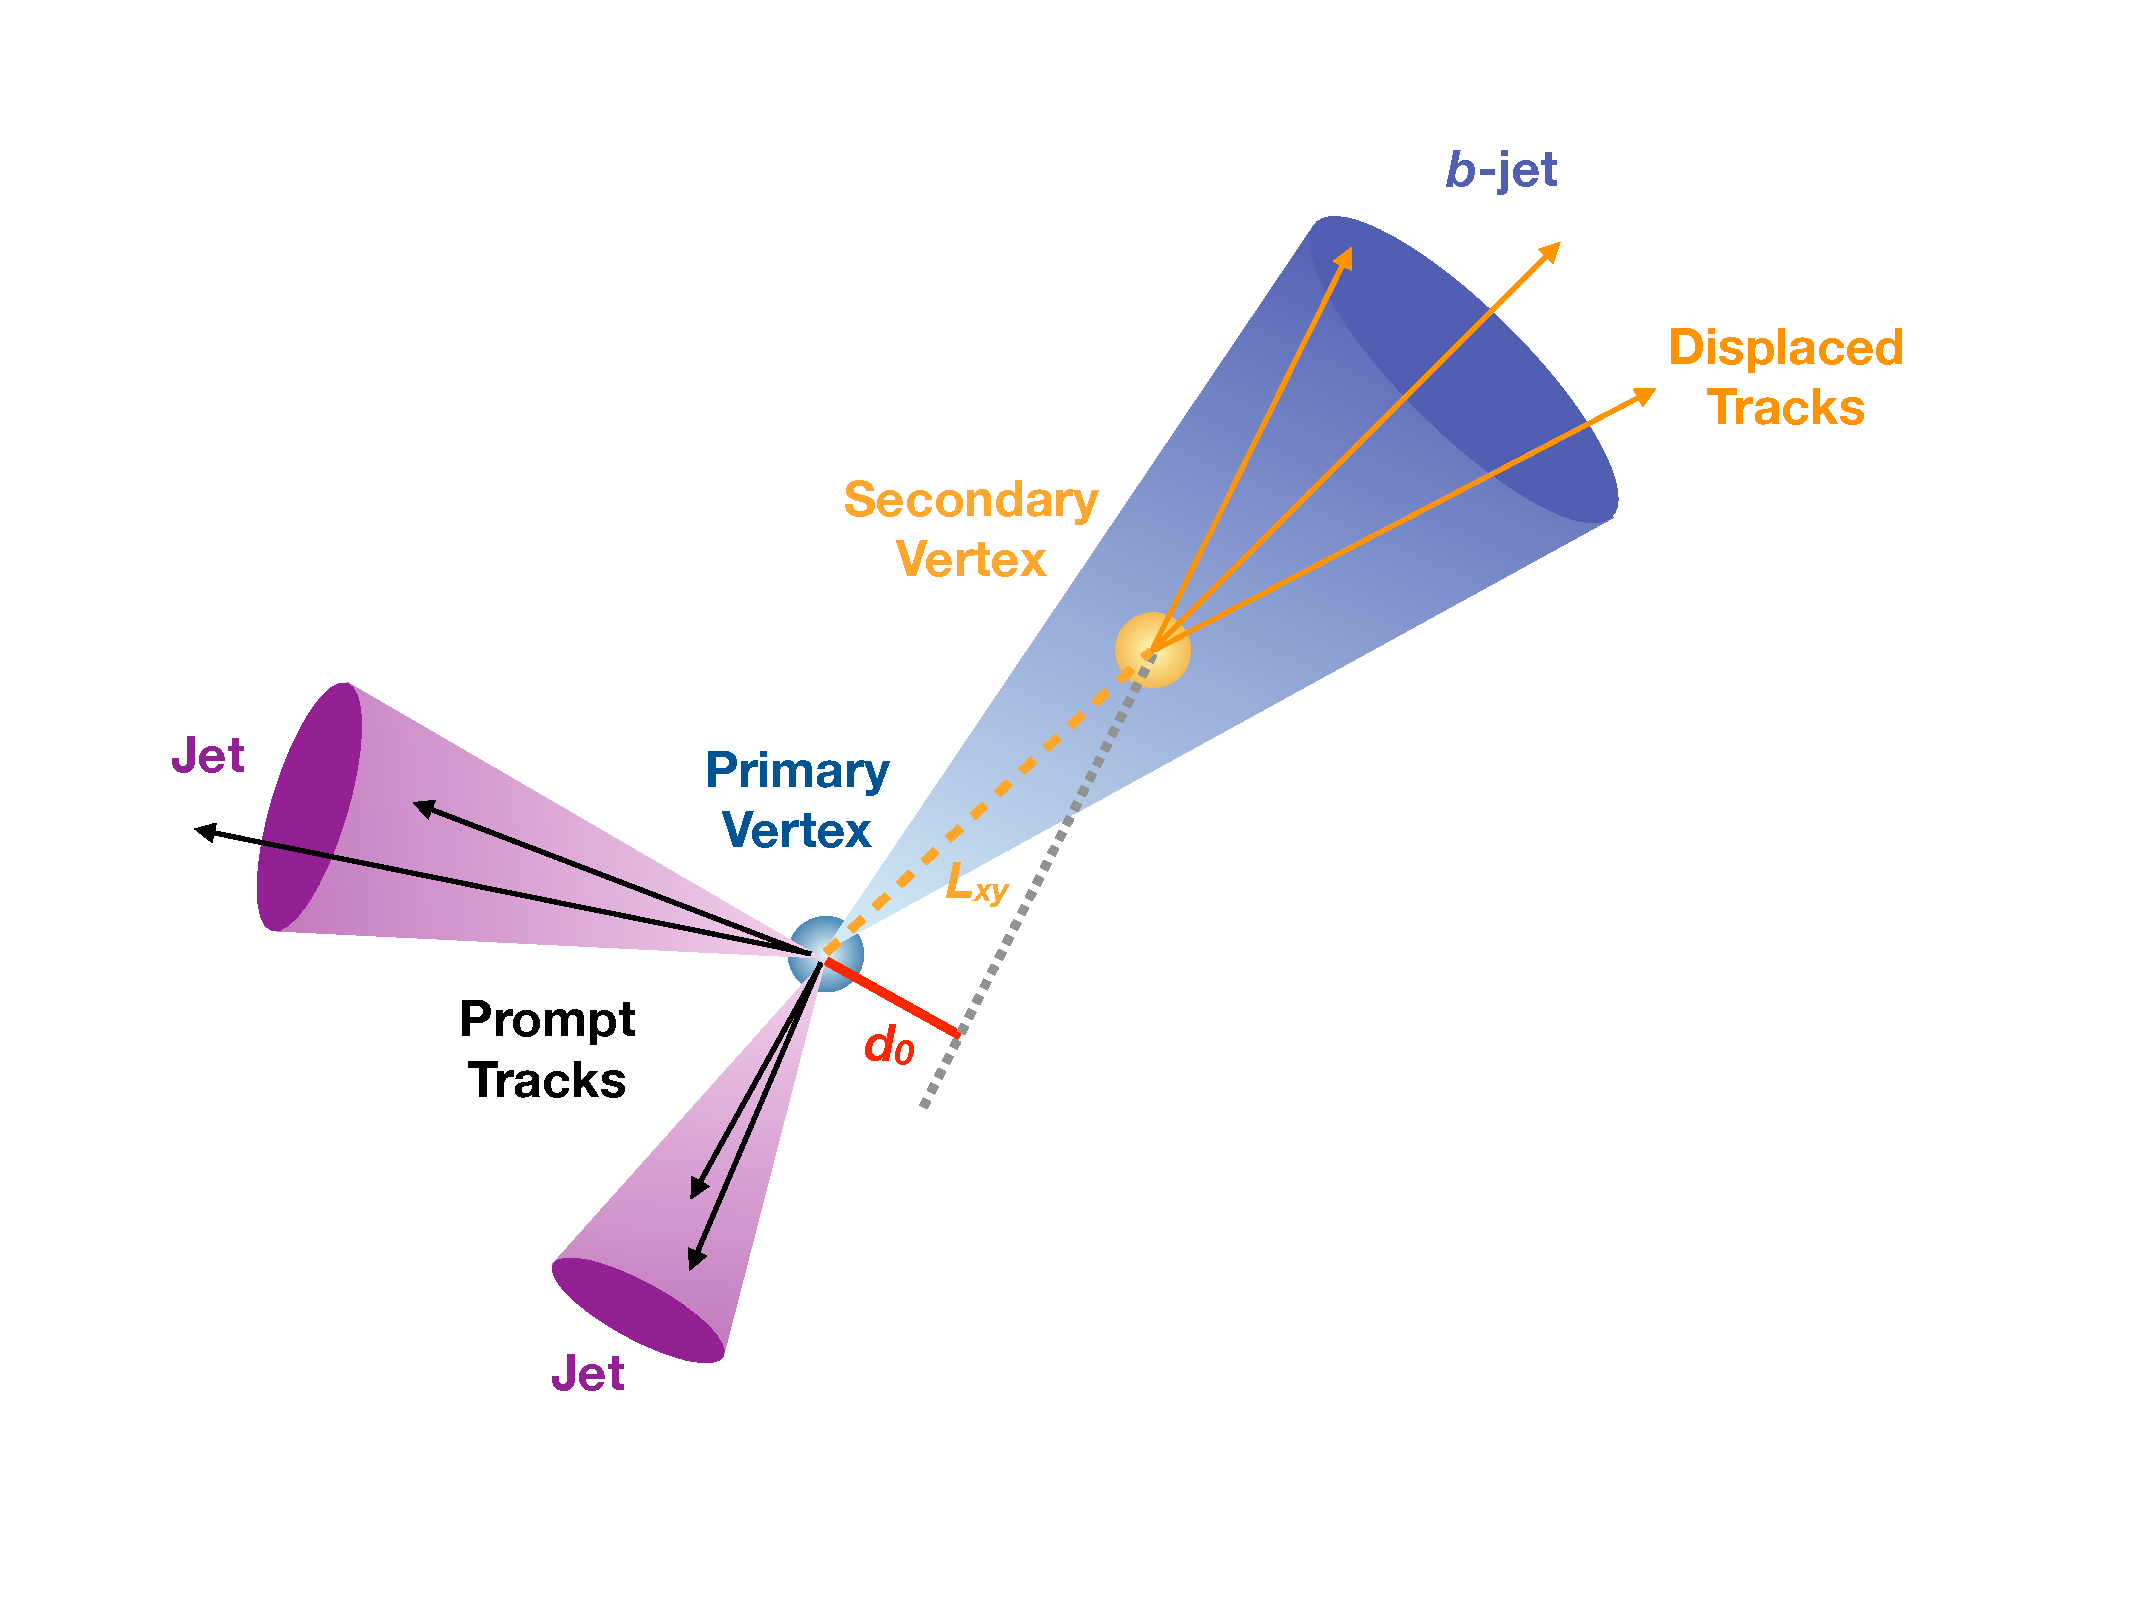
\includegraphics[width=0.7\textwidth]{figures/ftag/b-trig-paper/fig_01}
  \caption{Schematic illustration for the characteristic ``long'' lifetime of a \Pqb-hadron \cite{b-trig-paper}. }
  \label{fig:b-jet-graphic}
\end{figure}

The characteristically long lifetime of hadrons containing $b$-quarks ($b$-hadrons) of the order of 1.5 ps \cite{PDG} leads to two classes of $b$-tagging algorithms: \textit{vertexing} based algorithms which explicitly reconstruct a production point, or vertex, of the $b$-hadron decay displaced from the primary interaction point, and track based algorithms which exploit the displacement of the reconstructed charged particles trajectories (tracks) produced in $b$-hadron decays from the primary interaction point.

%We then use a NN to combine information from these low-level algorithms into a high level tagger and we refer to these collection of algorithm to solve the classification problem of identifying jets containing a $b$-quark as $b$-tagging.

\begin{figure}[htbp]
  \centering
  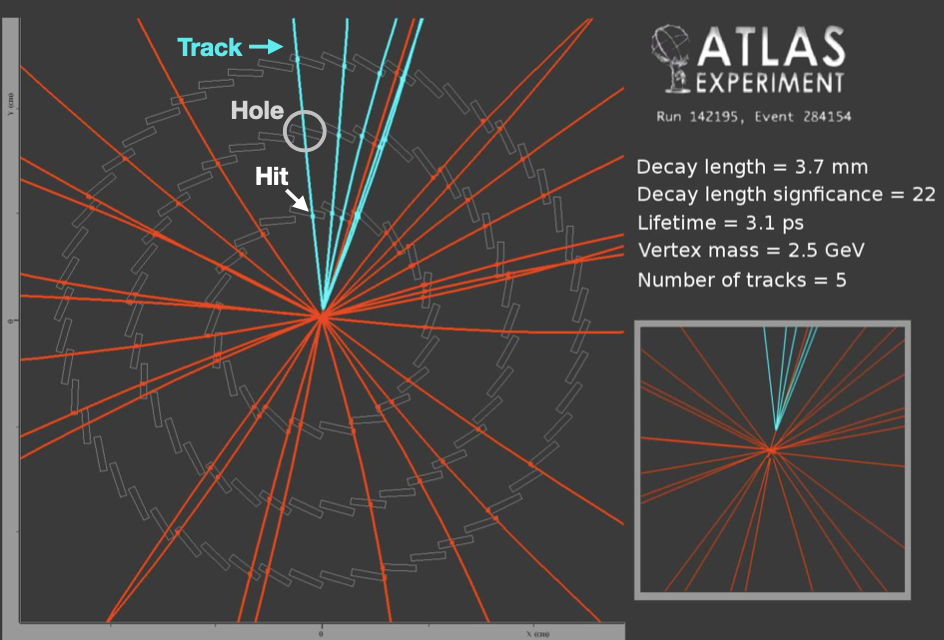
\includegraphics[width=0.9\textwidth]{figures/ftag/b-decay-evt-display-annotated}
  \caption{Illustration of what a b-decay looks like in the ATLAS detector. 
  The cyan colored lines illustrate the tracks from the \Pqb-hadron decay, and in the inset figure you can see the displacement of these tracks from the primary vertex. 
  Only three pixel layers are shown as this is a Run~1 event, and the IBL was not yet installed. \hl{Need to revise older notes to find where this event display came from (or ask Su Dong)}. }
  \label{fig:b-jet-graphic}
\end{figure}

To further set the stage for the problem of interest in this chapter, in \Fig{\ref{fig::jet-displays}} motivates what these weakly decaying hadrons look like in simulation that includes the truth information.
What we have as inputs to flavor tagging are the set of track features in the perigee representation with the IPs defined with respect to the point of closest approach (POCA). \Fig{\ref{fig::jet-displays}} shows these track parameters as we extrapolate out from the PV using the extrapolation equations defined in \Sect{\ref{sec:vertexing}}\footnote{Many thanks to Jonathan Shalomi for the nice track extrapolator code.}.
%The jet displays in \Fig{\ref{fig::jet-displays}} are EMTopo jets passing the standard jet selection cuts, and show all of the reconstructed tracks passing the loosest FTAG preselection. 
These representative images illustrate 
\begin{itemize}
	\item \textbf{\Pqb-jet:} There's a characteristic, tertriary decay of both the B and D hadrons.
	\item \textbf{\Pqc-jet:} There's a weakly decaying D-hadron, but closer to the PV than the weak decays in the \Pqb-jet.
	\item \textbf{light-jet:} Tracks are well collimated with the jet axis and most appear to be originating from the PV, although there are some tracks that that can appear to extrapolate to a point other than the PV.
\end{itemize}

\Tab{\ref{table:decay-length}} shows how often the B and D hadrons decay before the reaching either the first pixel sensor (the IBL) or even the edge of the beam pipe and illustrates that the power of the reconstructing the displaced vertex mostly is coming from the extrapolation.

\begin{table}[h!]
  \centering
    \begin{tabular}{l | l l  } % <-- Alignments: 1st column left, 2nd middle and 3rd right, with vertical lines in between
      {} & \textbf{B-hadron decays before} & \textbf{D-hadron decays before}  \\
      \hline
	Beam pipe &  2.1 \% & 0.3 \% \\
	IBL & 0.94 \% & 0.1 \%
    \end{tabular}
    \caption{Decay length of the weakly decaying hadron for jets in from a semi-leptontic $t\bar{t}$ sample.}
    \label{table:decay-length}
\end{table}

\begin{figure} 
\centering
\vspace{-1cm}
	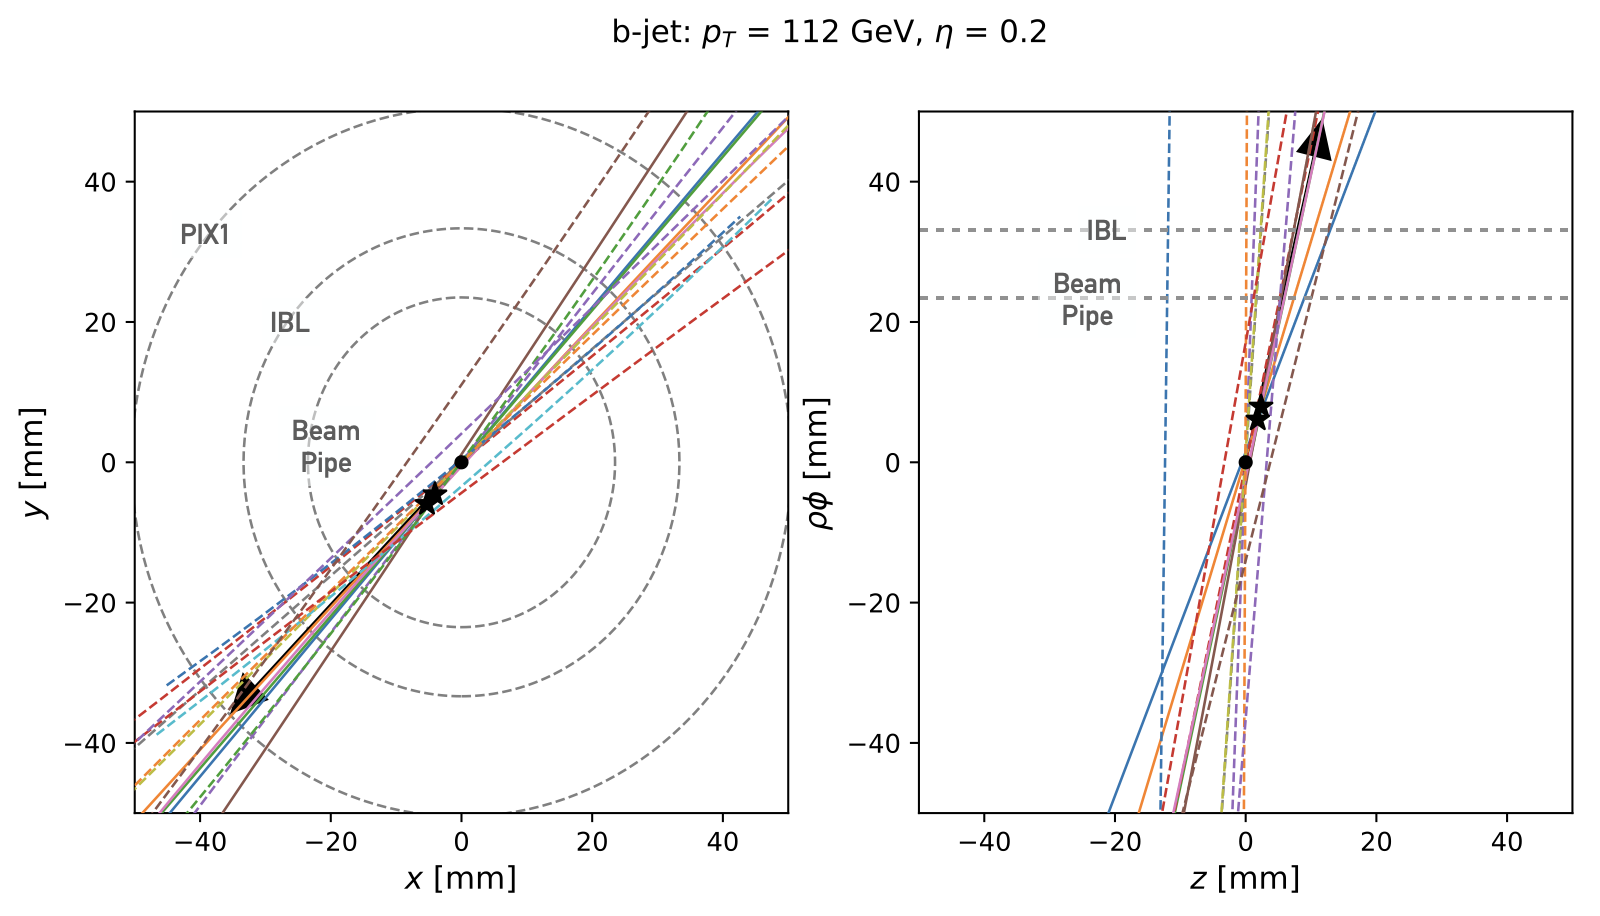
\includegraphics[height=2.75in]{{figures/ftag/jetDisplays/jet5}}
	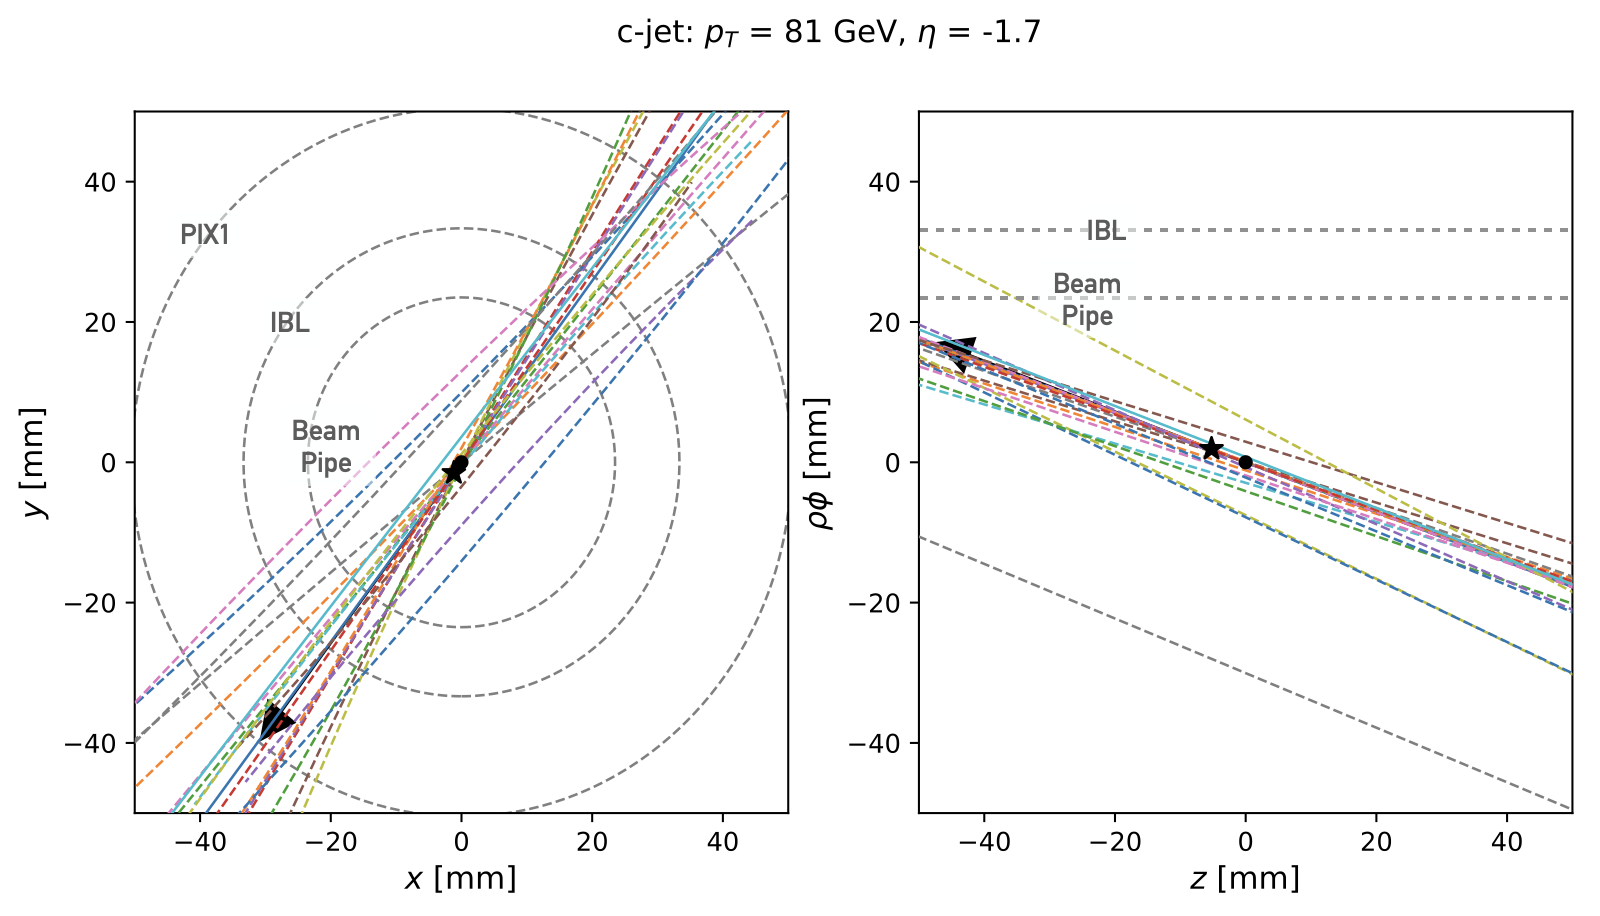
\includegraphics[height=2.75in]{{figures/ftag/jetDisplays/jet32}}
	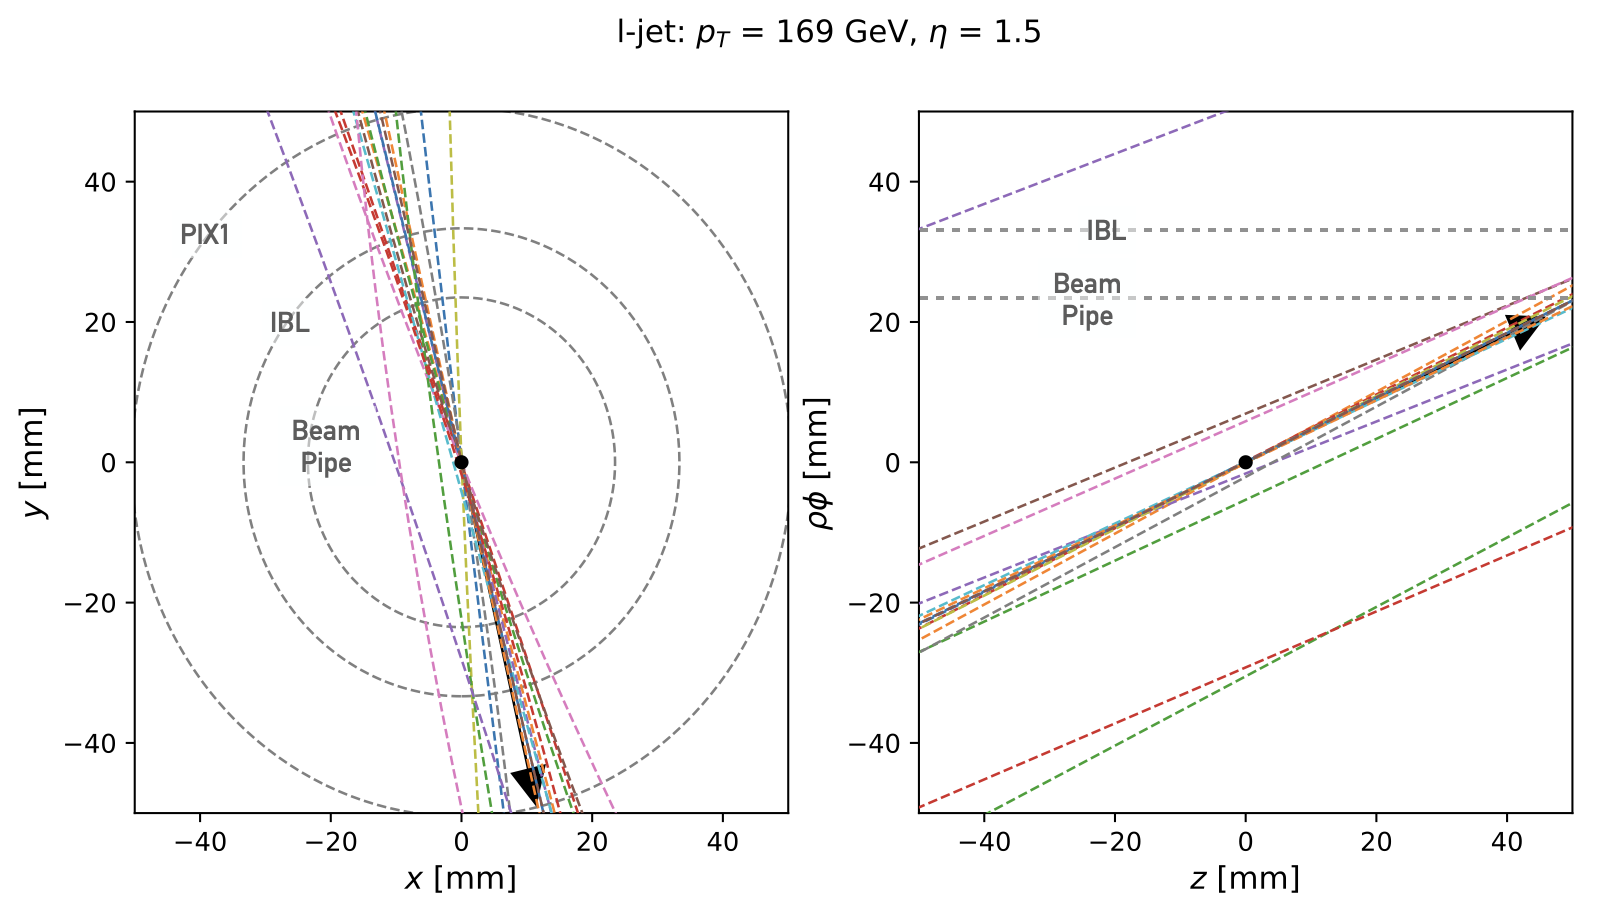
\includegraphics[height=2.75in]{{figures/ftag/jetDisplays/jet3}}
\caption{Visualization of the (x,y) and $(z,\rho\phi)$ 2d views of the tracks for reconstructing the secondary vertex (or vertices). 
The arrow on the figure indicates the jet axis, and a $\star$ shows where the weakly decaying hadron decays.
The solid lines are tracks from the HF decay, while the dashed lines denote the other tracks associated to the jet.}
\label{fig::jet-displays}
\end{figure}

\FloatBarrier
\clearpage

ATLAS employs several IP-based algorithms which are later combined with vertexing algorithms to produce a "high-level" tagger for general use.

\begin{figure}[htbp]
  \centering
  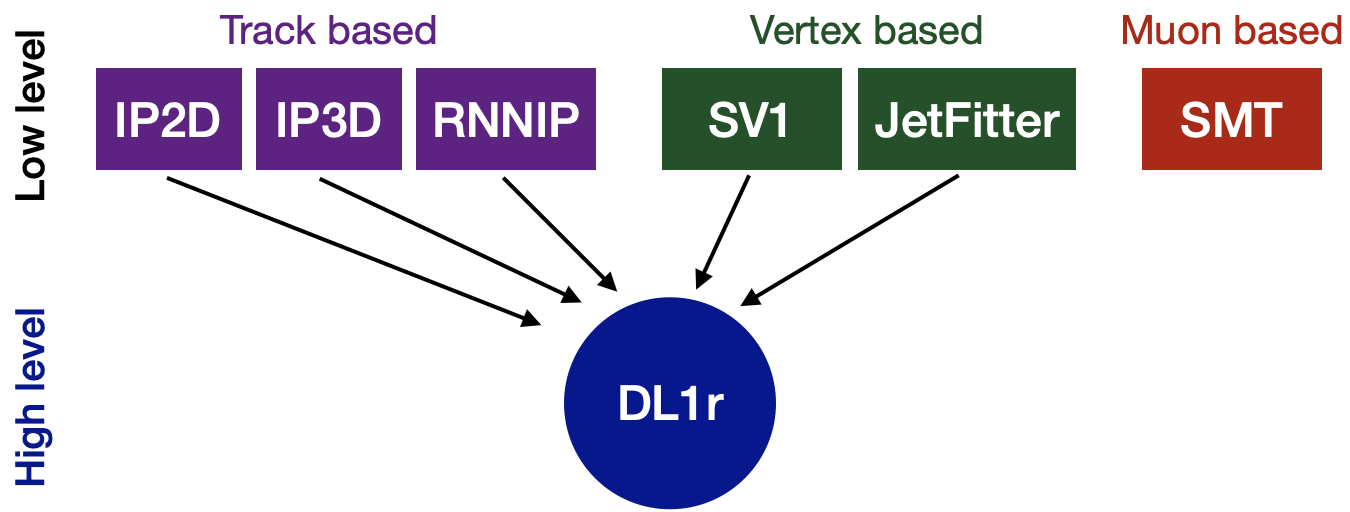
\includegraphics[width=0.9\textwidth]{figures/ftag/ATLAS-taggers}
  \caption{Types of \Pqb-taggers used on ATLAS}
  \label{fig:ATLAS-taggers}
\end{figure}

This chapter is organized as follows: Section \ref{sec:datasets} describes the datasets and selections used to train and evaluate the algorithms, while section \ref{sec:alg} details impact parameter based taggers, the Deep Sets algorithm and our specific implementation. Section \ref{sec:results} shows investigations of what the network has learned, results for the timing metrics, discussion on calibrating the algorithm, and the optimization studies conducted. Finally, section \ref{sec:conclusion} summarizes the conclusions.


\section{Datasets (?)}
\label{sec:intro}

Algorithm training and evaluation is performed with simulated $t\bar{t}$ events, produced by $\sqrt{s} = 13$~TeV proton-proton collisions, in which at least one of the W bosons, from the top quark decay, decays leptonically. 
Events are generated using the
\powhegbox~\cite{Frixione:2007nw, Nason:2004rx, Frixione:2007vw, Alioli:2010xd}~v2
generator at next-to-leading order with the NNPDF3.0NLO~\cite{Ball:2014uwa} parton set
of distribution functions~(PDF) and the \hdamp\ parameter\footnote{The
  \hdamp\ parameter is a resummation damping factor and one of the
  parameters that controls the matching of Powheg matrix elements to
  the parton shower and thus effectively regulates the
  high-\pt\ radiation against which the \ttbar\ system recoils.} set
to 1.5~\mtop~\cite{ATL-PHYS-PUB-2016-020}, with $\mtop = 172.5$ GeV.  The events are interfaced
to \pythia.230~\cite{Sjostrand:2014zea} to model the parton shower,
hadronisation, and underlying event, with parameters set according
to the A14 tune~\cite{ATL-PHYS-PUB-2014-021} and using the \nnpdftwo
set of PDFs~\cite{Ball:2012cx}. The decays of $b$ and $c$-hadrons
are performed by \evtgen~v1.6.0~\cite{Lange:2001uf}.
Particles are passed through the ATLAS detector simulation \cite{SOFT-2010-01} based on GEANT4 \cite{Agostinelli:2002hh}.

Jets are reconstructed from particle flow objects \cite{PERF-2015-09} using the anti-$k_T$ algorithm \cite{Cacciari:2008gp} with $R=0.4$. 
The jet energy scale is calibrated according to \cite{PERF-2016-04}.
Jets used for training and evaluation have $\pT \geq 20$ GeV, $|\eta|$ < 2.5, and are required not to overlap with a generator-level electron or muon from W boson decays. 
Additionally, the contamination of jets from other interactions in the beam crossing (pile-up) is surpressed by applying the jet vertex tagger \cite{ATLAS-CONF-2014-018} optimized for particle flow jets. 
%, jets with $\pT$ < 60 GeV and $|\eta|~>~2.4$ are removed if failing a jet vertex tagging (JVT) requirement that has an efficiency of 92\% for jets originating from the hard scatter vertex, with a residual rate of pile-up jets of approximately 2\%

Tracks are associated to jets using a $\Delta R$ association cone which decreases as a function of jet $\pT$, with a maximum association $\Delta R$(track, jet) of approximately 0.45 for a jet with $\pT = 20$~GeV and $\Delta R$(track, jet) of approximately 0.25 when the jet $\pT = 200$~GeV. 
If a track is within the association cones of more than one jet, it is assigned to the jet which has a smaller $\Delta R$(track, jet).

The impact parameter of the track characterises the point-of-closest approach of a track to the PV in the longitudinal ($z_0\sin \theta$) and transverse ($d_0$) planes. 
Of particular use in $b$-tagging is the IP significance defined as the impact parameter divided by its uncertainty, $s_{d0} = d_0 / \sigma_{d0}$ and $s_{z0} = z_0 \sin \theta / \sigma_{z0 \sin \theta}$. 
% The \textit{lifetime sign} is used to sign the 
The track's IP and its significance are signed according to the track's direction with respect to the jet axis and the primary vertex~\cite{PERF-2012-04}. A positive IP is expected to be consistent with a track produced from a displaced vertex. 
This procedure is referred to as lifetime signing.
%, as it aids in characterising whether the track is more likely to come from a long lived hadron or a wrongly associated tracks. \textbf{NEED LIFETIME SIGN DEFINITION}. 
The nominal track selection considered in the algorithms to be described requires tracks with $\pT  > 1$ GeV,  $|d_0| < 1$ mm, and  $|z_0 \sin \theta | < 1.5$ mm.
% We consider two track $\pT$ and IP selections for the tracks in the training. The first is the tight selection of the RNNIP algorithm with $\pT  > 1$ GeV,  $|d_0| < 1$ mm, and  $|z_0 \sin \theta | < 1.5$ mm. The second is a looser selection with $\pT$ > 500 MeV, $|d_0| <$ 3.5 mm and $|z_0 \sin \theta | <$ 5 mm.

The jets are labelled as $b$-jets if they are matched to at least one $b$-hadron having $\pT \geq 5$ GeV within $\Delta R$($b$-hadron, jet)$< 0.3$ of the jet axis. 
If this condition is not satisfied, then $c$-hadrons and then $\tau$ leptons are searched for, with similar selection criteria.
If a jet is matched to a $c$-hadron ($\tau$-lepton), it is labelled a $c$-jet ($\tau$-jet).
%,  within 0.3 of the jet axis, the jet is labelled as a $c$-jet. Jets not identified as $b$- or $c$-jets but with a $\tau$-lepton within 0.3 of the jet axis are given a $\tau$ label. 
A jet that does not meet any of these conditions is called a light-flavour jet.%, which can include jets initiated by $u$- $d$-, and $s$-quarks or gluons, although there are some residual PU jets that can leak into this category as well.

%For RNNIP, we compared training with and without a dedicated output node for jets in the $\tau$ class, but as the $\tau$ class did not improve our $b$-tagging performance, we show experiments for the network trained only on $b$, $c$, and $l$-jets.\footnote{Should I include these with and without $\tau$ node plots in the appendix?}

%textbf{Note w/ the fakes issue that Nick Style's was talking about, we will have fake tracks leaking into our fragmentation category.}


\FloatBarrier
\clearpage
\section{Low level taggers}

\subsection{IPXD}
\subsection{SV1}
\subsection{JetFitter}
\subsection{SMT}

\FloatBarrier
\clearpage
\section{Recommendations for Run 2 b-taggers}

\subsection{High level taggers: DL1 series}

We combine the low level taggers into a high-level one, the DL1r algorithm, combining information from the low-level taggers:
\begin{itemize}%[noitemsep]
	\item The IP2D and IP3D: $\log p_b$
	\item The RNNIP outputs: $p_b$, $p_c$, and $p_l$
	\item The SV1 vertex information (variables in \Tab{\ref{tab:sv1-inputs}})
	\item The JF displaced vertices characteristics, \Tab{\ref{tab:sv1-inputs}}.
\end{itemize} 


The comparisons that we'll show are again

\begin{itemize}
%\itemsep{0em}
	\item Explain architecture, optimization
	\item Explain default values
	\item pre-processing:  mean 0 and standard deviation 1 (except for the binary check variables)
\end{itemize} 

\subsection{Evaluating tagger performance}


\subsection{PFlow optimization}

\textbf{Hybrid sample definition}

In the course of the completion of this thesis, the collaboration switched from using EMTopo jets (which reconstruct a jet from the topo clusters in the calorimeter) to  using PFlow jets which cluster a jet using particle flow candidates that takes into account the better resolution of the tracker for reconstructing lower momentum objects. This improves the jet reconstruction algorithm in two ways. (1) We gain a better reconstruction of the jet \pt resolution (shown by 

\begin{itemize}
	\item Switching from EMTopo to PFlow
	\item Main improvement that we expected for $b$-tagging would be better with the better angular resolution for the jet axis
\end{itemize}

\begin{figure}[htbp]
  \centering
  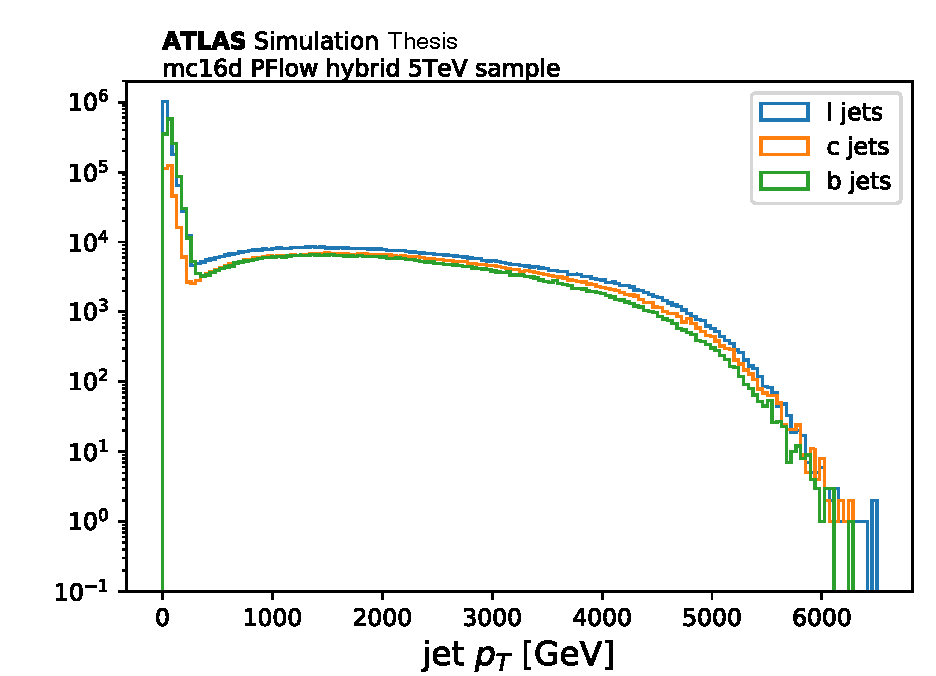
\includegraphics[width=.6\textwidth]{figures/ftag/PFlow trainings/pflow-pt-extended-hybrid}
  \caption{The \pt spectrum for training the Full Run 2 FTAG recommendations.}
  \label{fig:pflow-pt-extended-hybrid}
\end{figure}



\textbf{RNNIP optimization}

An illustration of why the task of \Pqb-tagging becomes harder at high \pt is illustrated in \Fig{\ref{fig:hf-ftag-tracks}}.


\begin{figure}[htbp]
  \centering
  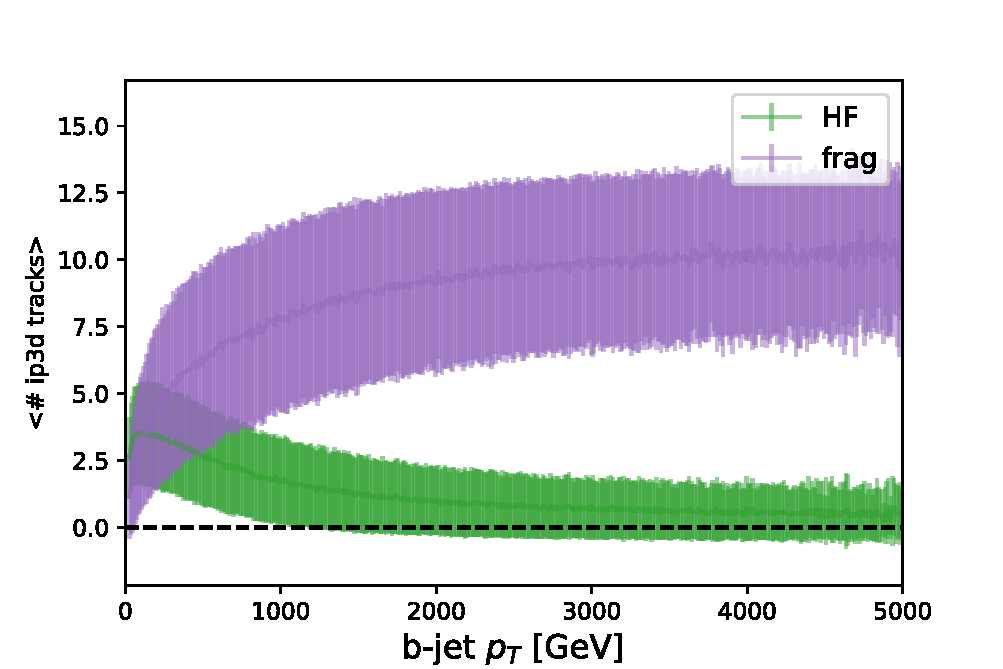
\includegraphics[width=.6\textwidth]{figures/ftag/PFlow trainings/hf-frag-tracks}
  \caption{The evolution of heavy flavor compared to the number of fragmentation tracks that have $\pt > 1~\mathrm{GeV}$, $|d_0| < 1$~mm, $|z_0 \sin \theta < 1.5$~mm, .}
  \label{fig:hf-frag-tracks}
\end{figure}


Our optimization for the RNNIP training for the PFlow tagger uses 400 hidden units in the \ldots LSTM cell.
This is an increase from the 50 hidden units of \cite{ATL-PHYS-PUB-2017-003} since training over the much larger dynamic range needed a more complex architecture.
\textbf{Do I remember what lr I used?}
The training was done with the adam optimizer, using 5 million jets, and 20\% of the dataset was held out as a validation set, and the training was stopped when the validation loss had not improved in the last 20 epochs.


\begin{figure}
\centering
\subfloat[light rejection]{
	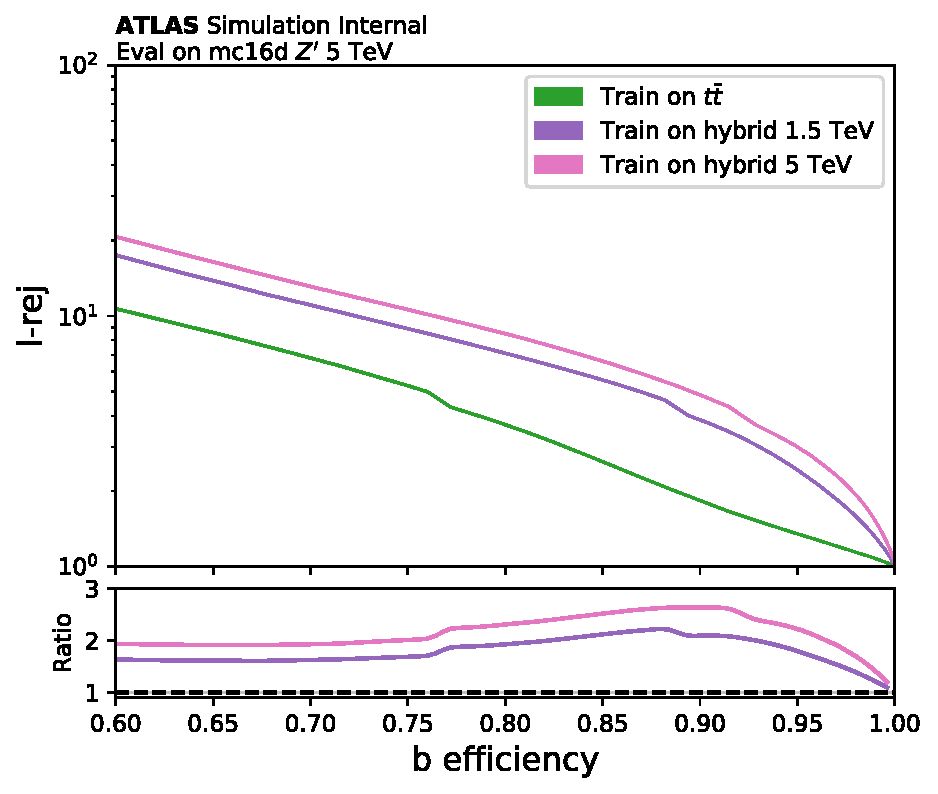
\includegraphics[width=0.45\textwidth]{{figures/ftag/PFlow\ Trainings/Zprime-l-roc}}
	}
\subfloat[\Pqc rejection]{
	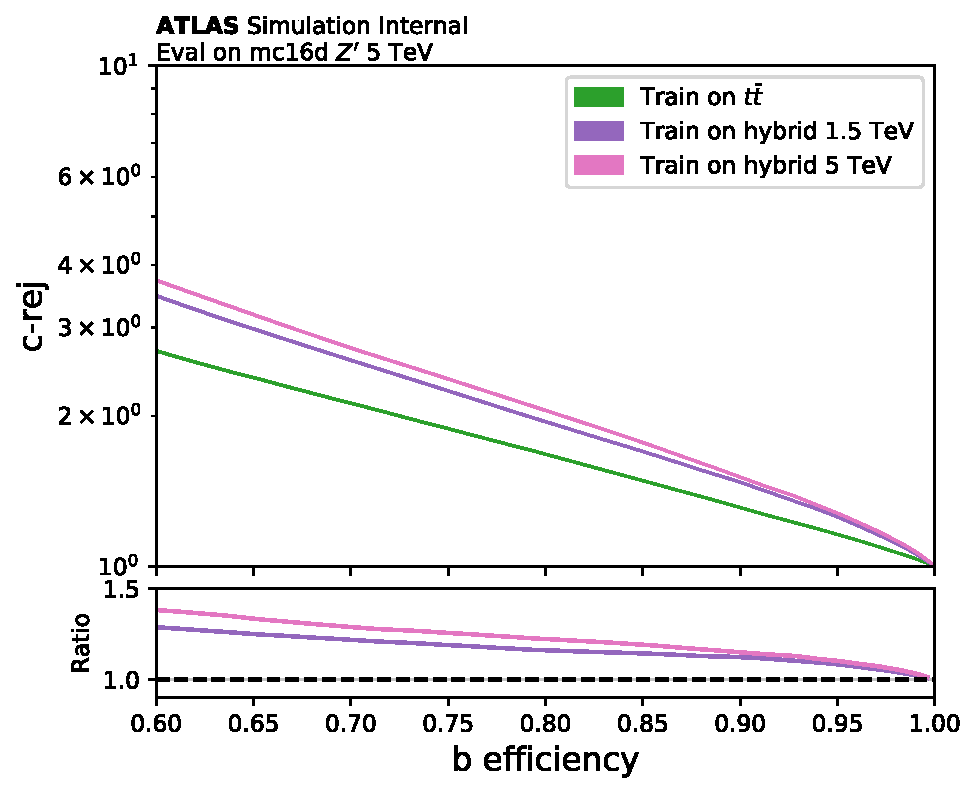
\includegraphics[width=0.45\textwidth]{{figures/ftag/PFlow\ Trainings/Zprime-c-roc}}
	}
\caption{}
\label{fig:Zprime-c-roc}
\end{figure}


\begin{figure}
\centering
\subfloat[light rejection]{
	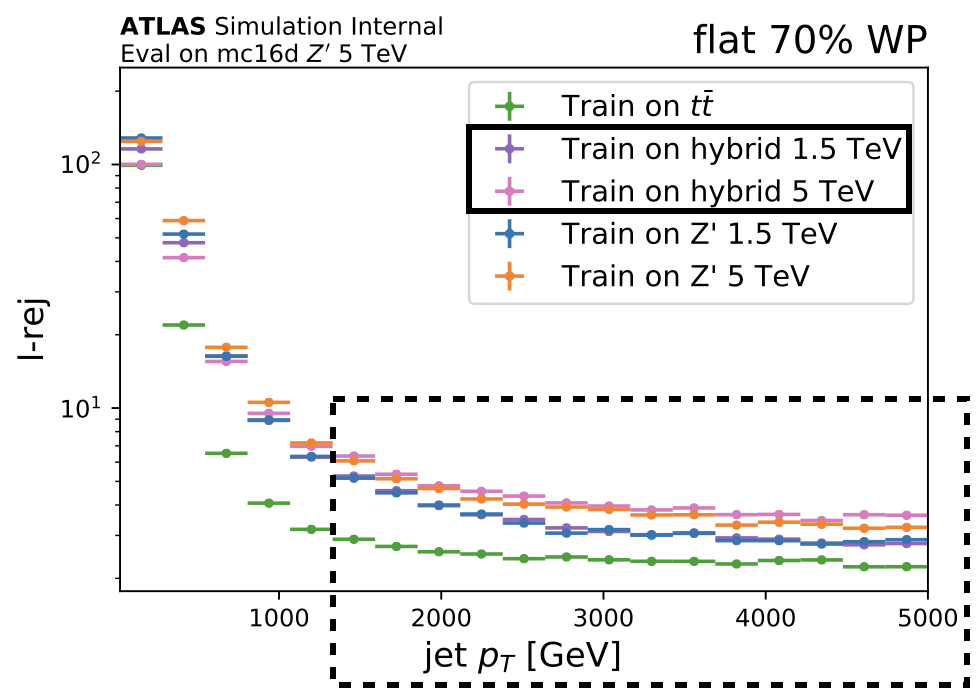
\includegraphics[width=0.45\textwidth]{{figures/ftag/PFlow\ Trainings/Zprime-l-pt}}
	}
\subfloat[\Pqc rejection]{
	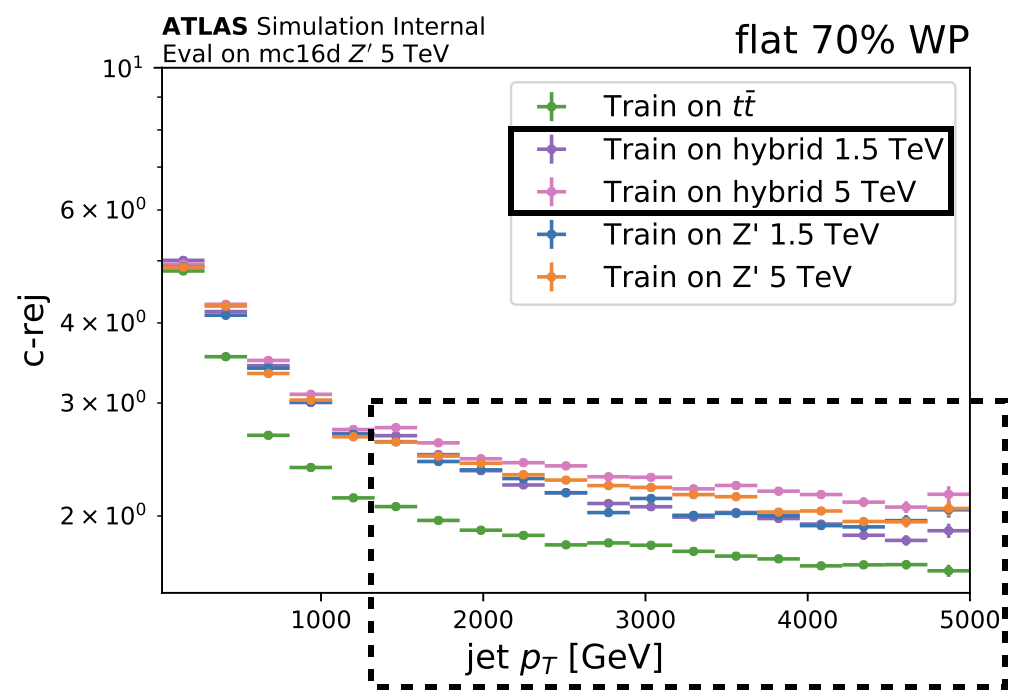
\includegraphics[width=0.45\textwidth]{{figures/ftag/PFlow\ Trainings/Zprime-c-pt}}
	}
\caption{}
\label{fig:Zprime-pt}
\end{figure}



\begin{figure}
\centering
\subfloat[light rejection]{
	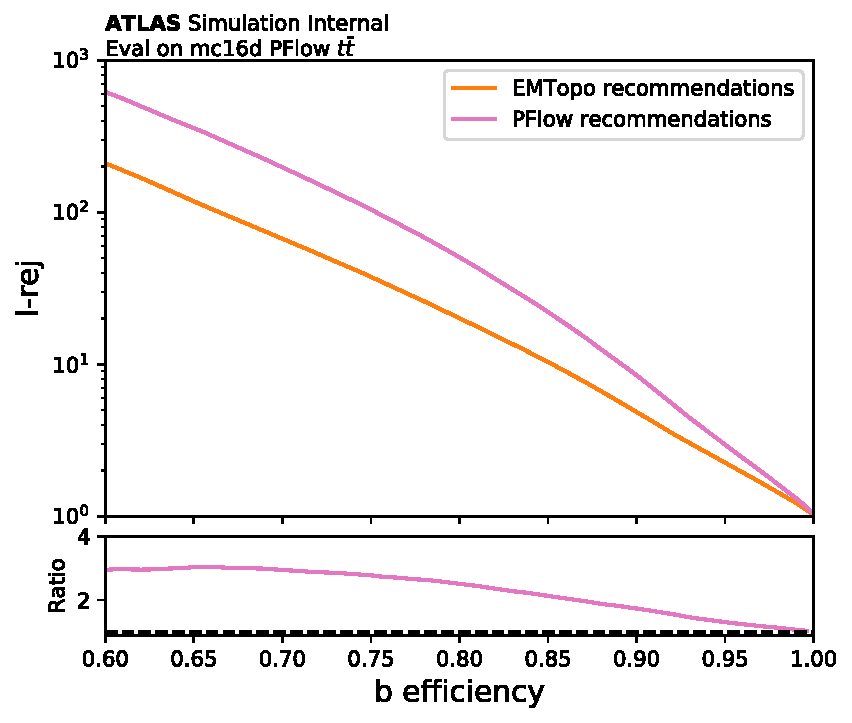
\includegraphics[width=0.45\textwidth]{{figures/ftag/PFlow\ Trainings/topo-vs-pflow-l-rej}}
	}
\subfloat[\Pqc rejection]{
	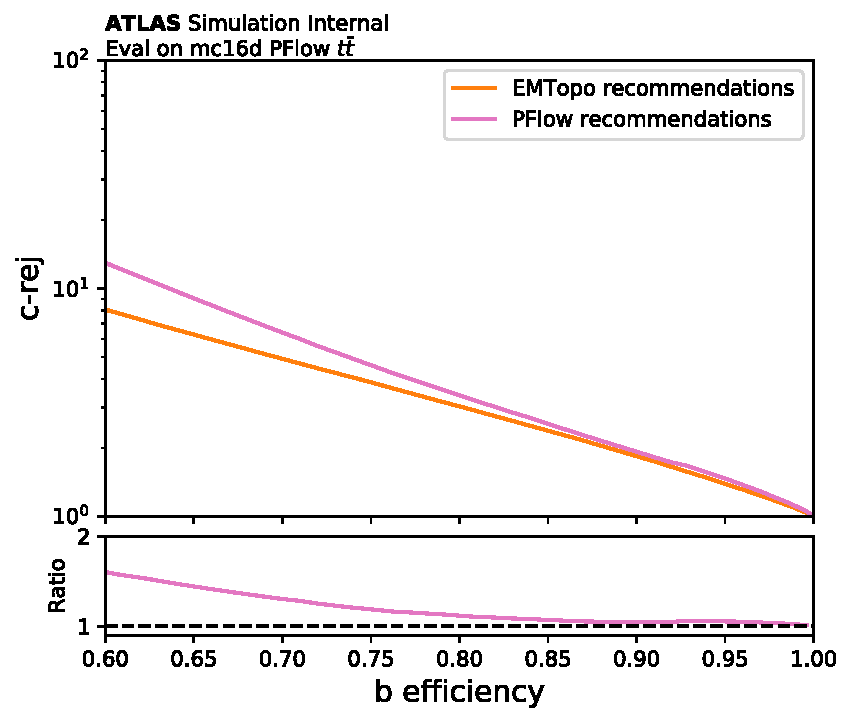
\includegraphics[width=0.45\textwidth]{{figures/ftag/PFlow\ Trainings/topo-vs-pflow-c-rej}}
	}
\caption{}
\label{fig:topo-pflow}
\end{figure}

The EMTopo training recommendation was from the 2017 retraining campaign:

Rafael showed we see retraining gains due to the kinematics changes with hdamp from mc15 -> mc16

Dedicated retraining on new pflow jet collection

Plus the RNN improvements from this year




\textbf{DL1r results}


% PFlow results link
% http://atlas.web.cern.ch/Atlas/GROUPS/PHYSICS/PLOTS/FTAG-2019-005/
\def\jetdef{PFlow}
\def\figpath{figures/ftag/\jetdef \ trainings}

\begin{figure}[htbp]
    \centering
    % light
    \subfloat[]{ 
            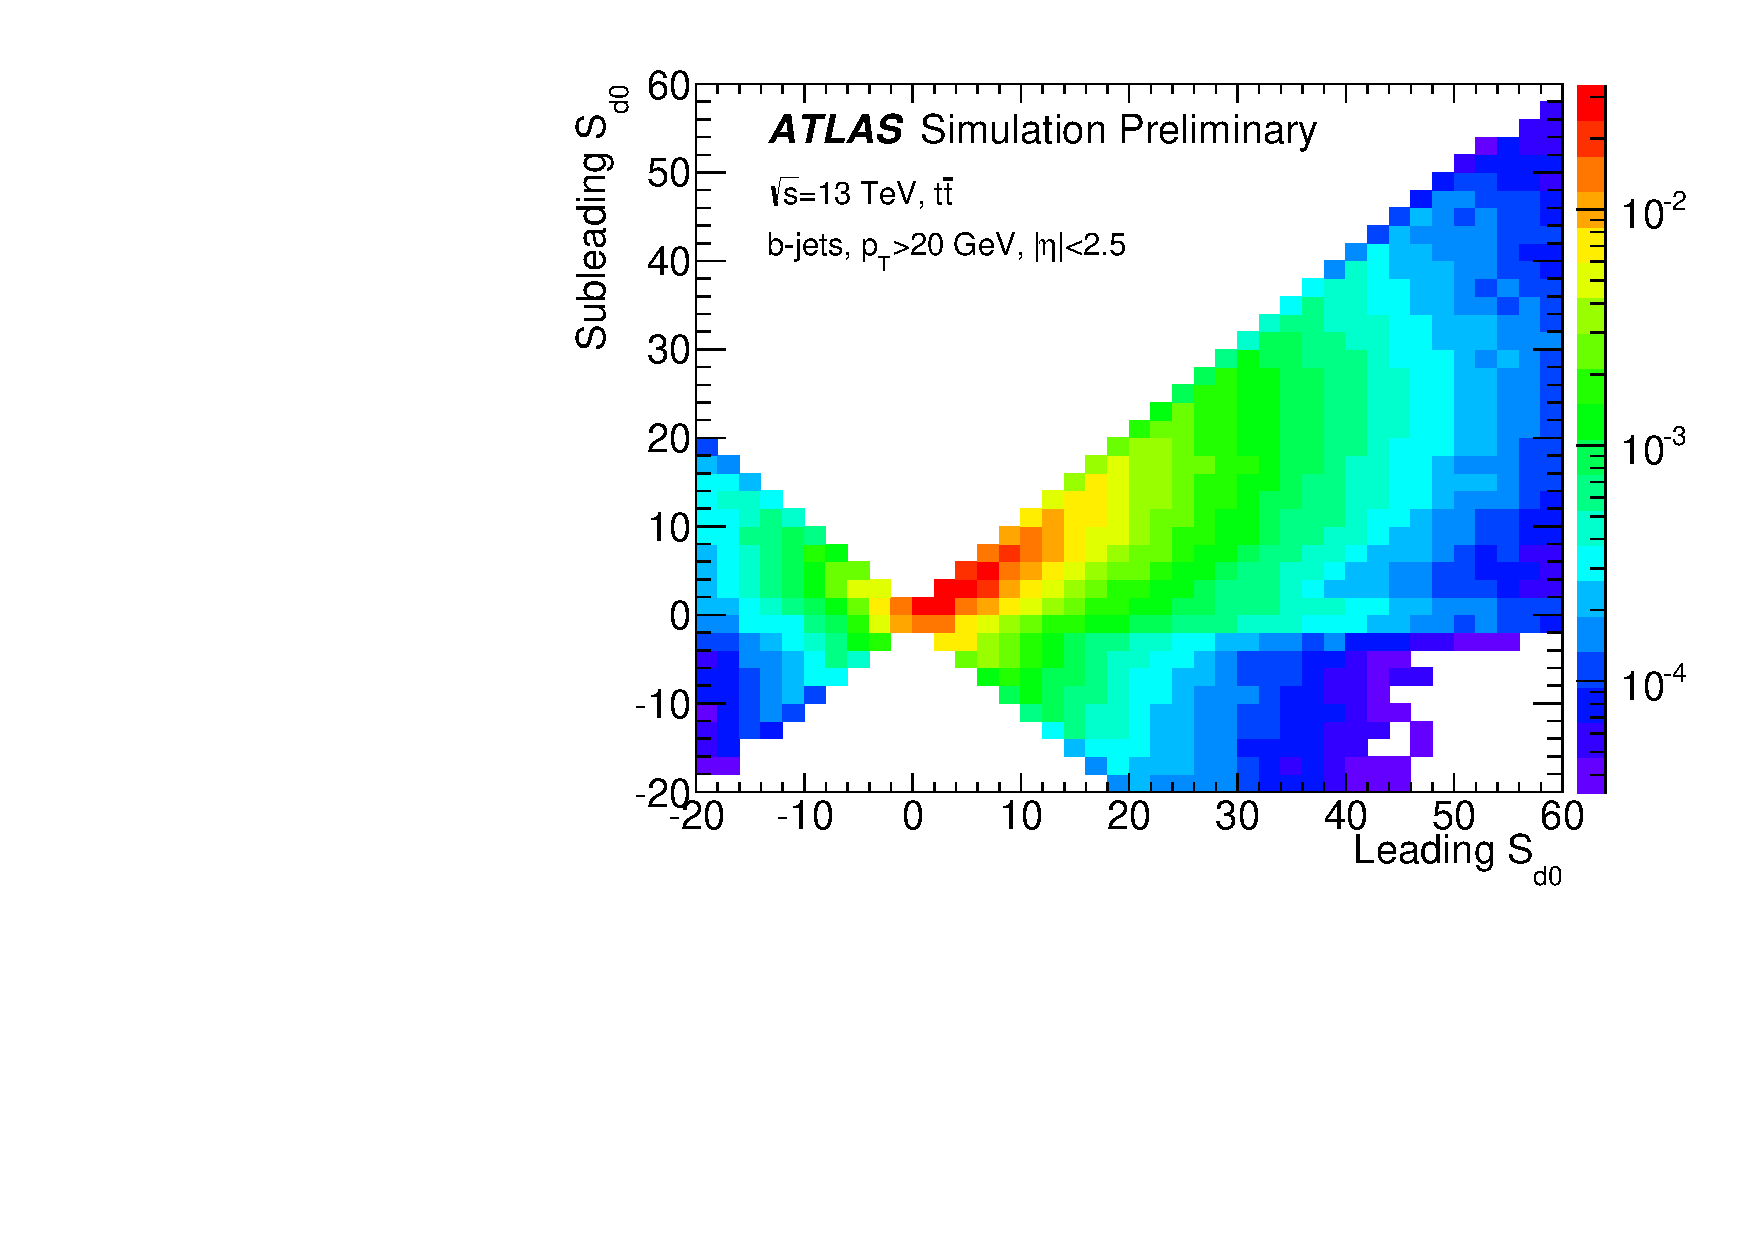
\includegraphics[width=0.48\linewidth]{\figpath/fig_01a}
    } 
     \subfloat[]{ 
            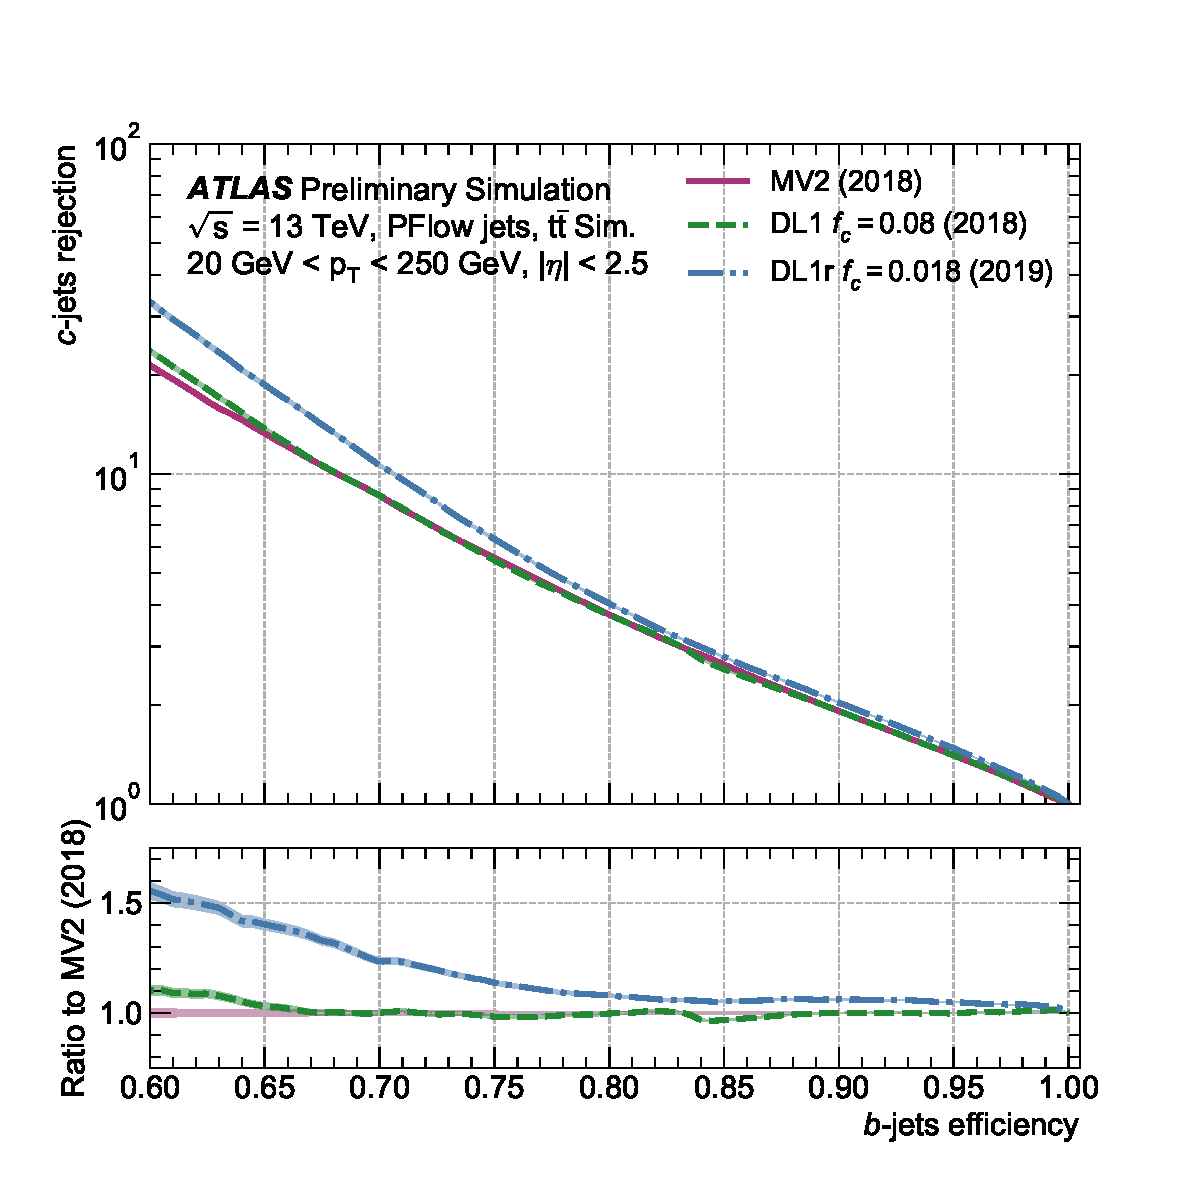
\includegraphics[width=0.48\linewidth]{\figpath/fig_01b}
    } 
    \caption{}
    \label{fig:\jetdef-fig1}
\end{figure}

\begin{figure}[htbp]
    \centering
    % light
    \subfloat[]{ 
            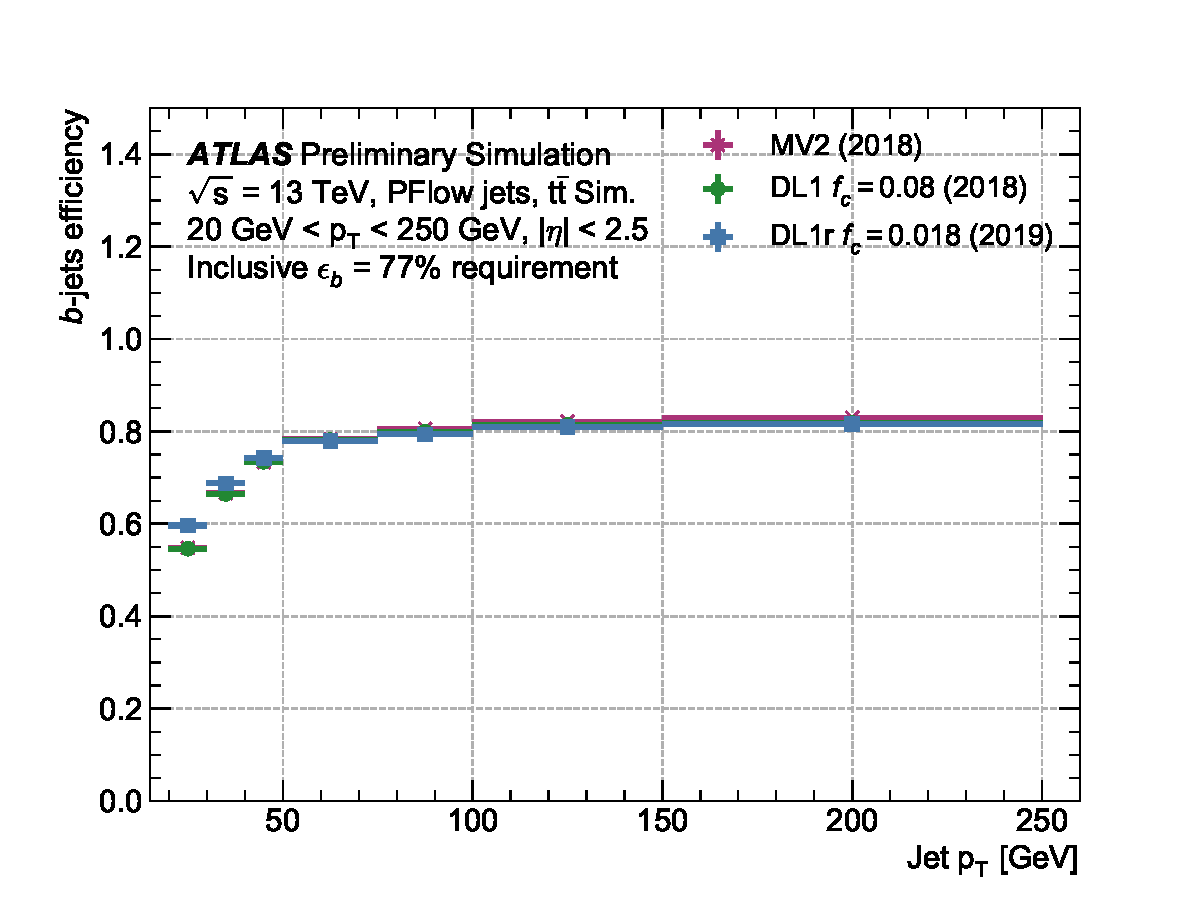
\includegraphics[width=0.33\linewidth]{\figpath/fig_02a}
    } 
     \subfloat[]{ 
            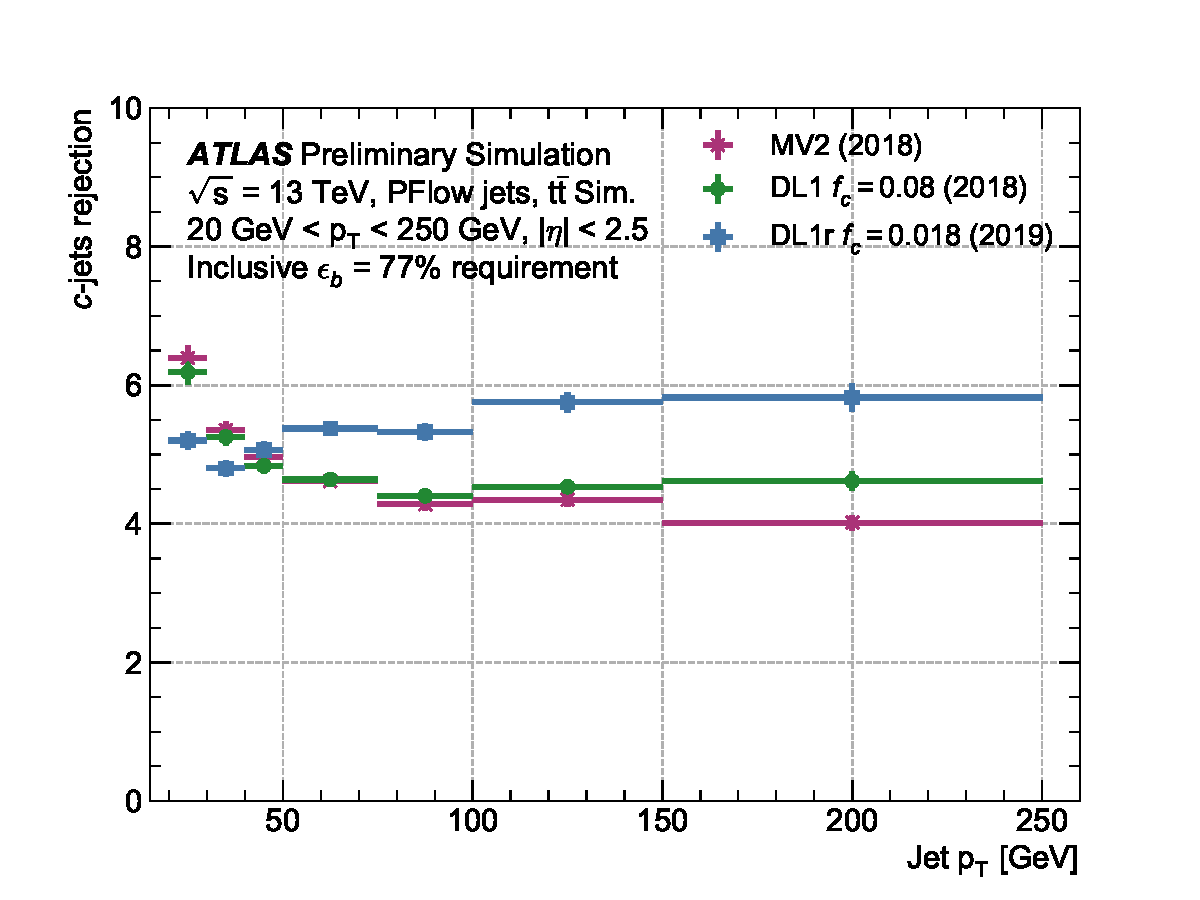
\includegraphics[width=0.33\linewidth]{\figpath/fig_02b}
    } 
    \subfloat[]{ 
            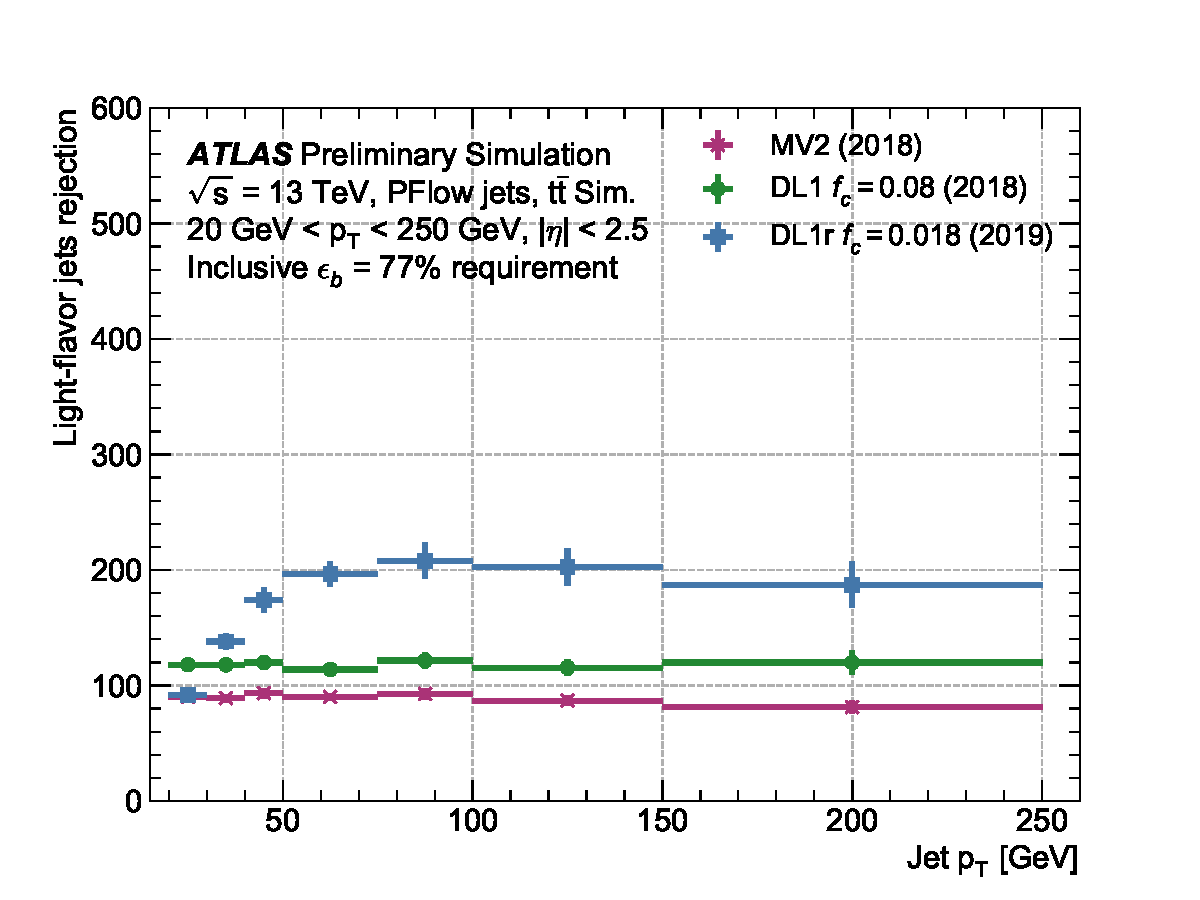
\includegraphics[width=0.33\linewidth]{\figpath/fig_02c}
    } 
    \caption{}
    \label{fig:\jetdef-fig2}
\end{figure}

\begin{figure}[htbp]
    \centering
    % light
    \subfloat[]{ 
            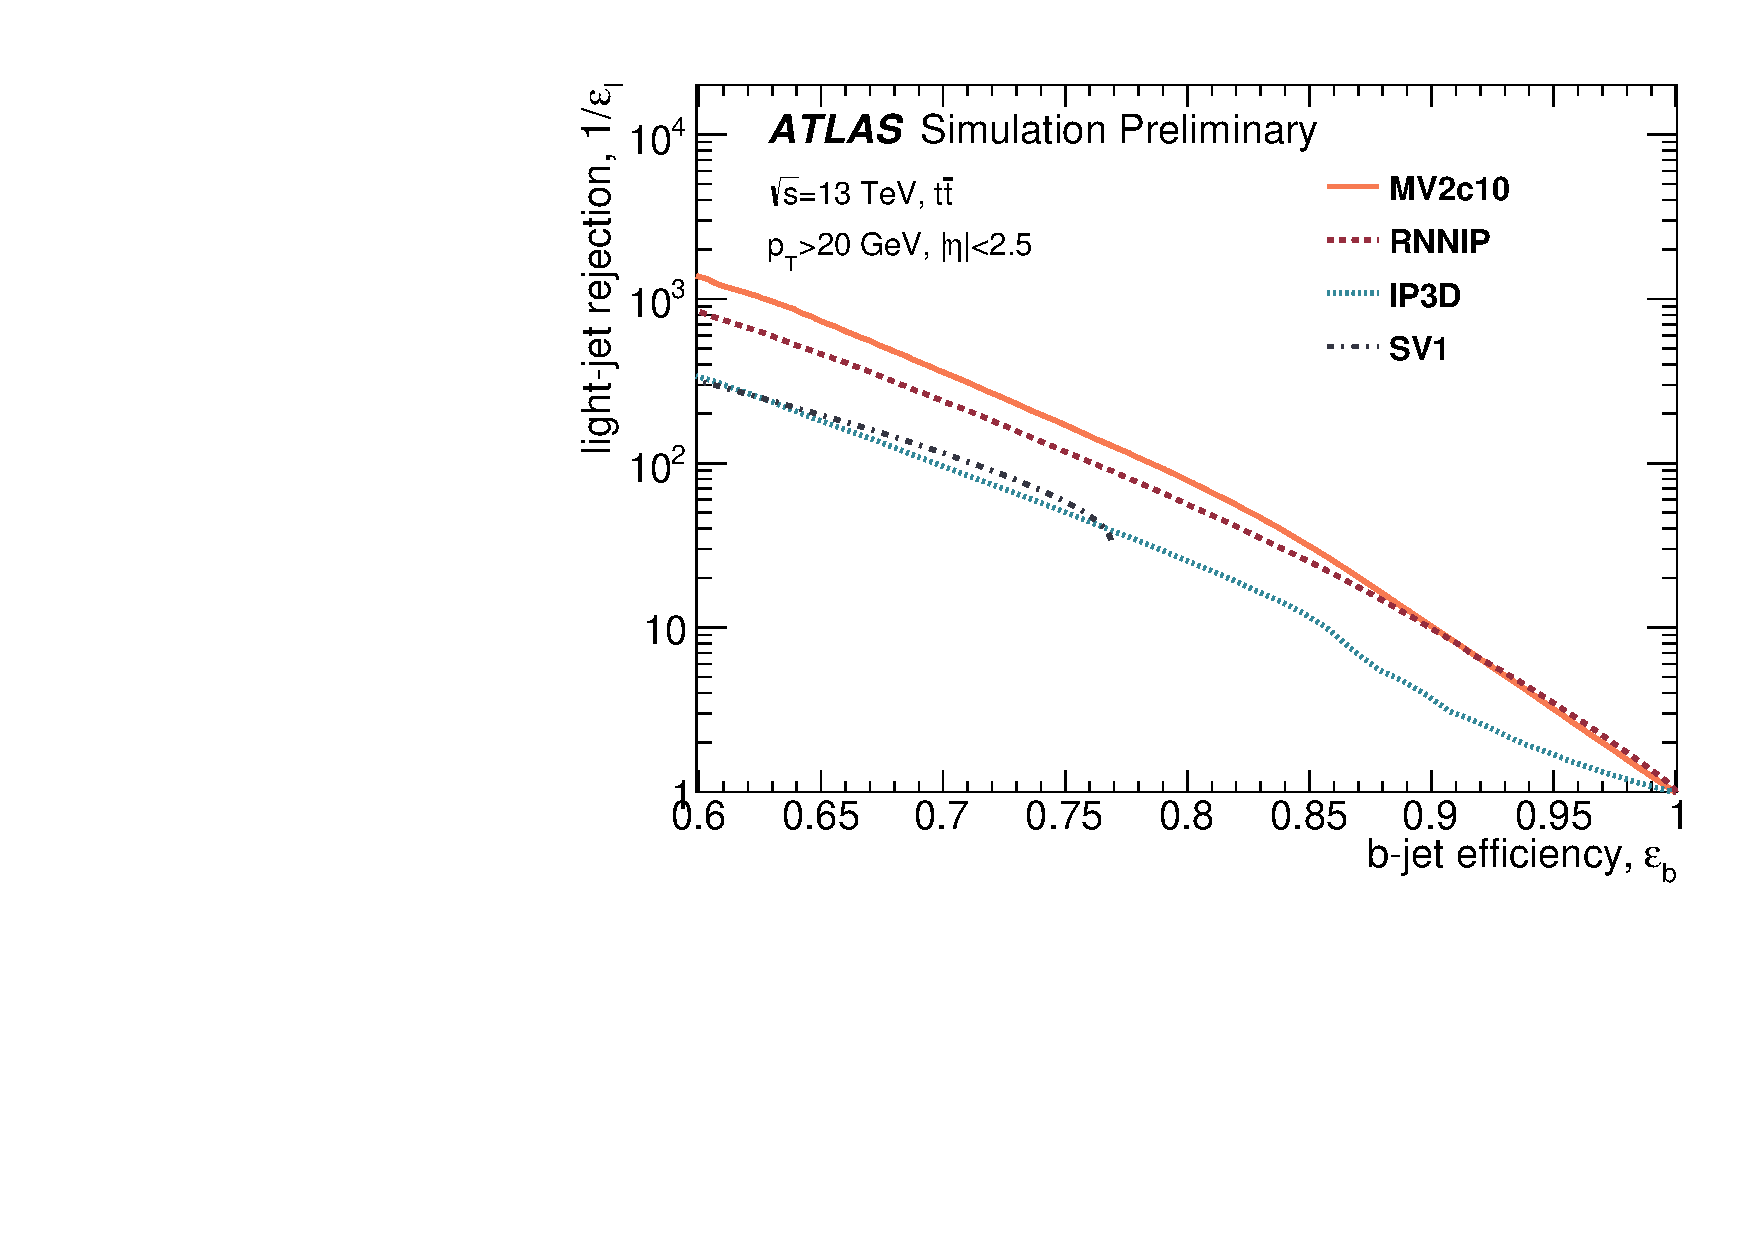
\includegraphics[width=0.48\linewidth]{\figpath/fig_03a}
    } 
     \subfloat[]{ 
            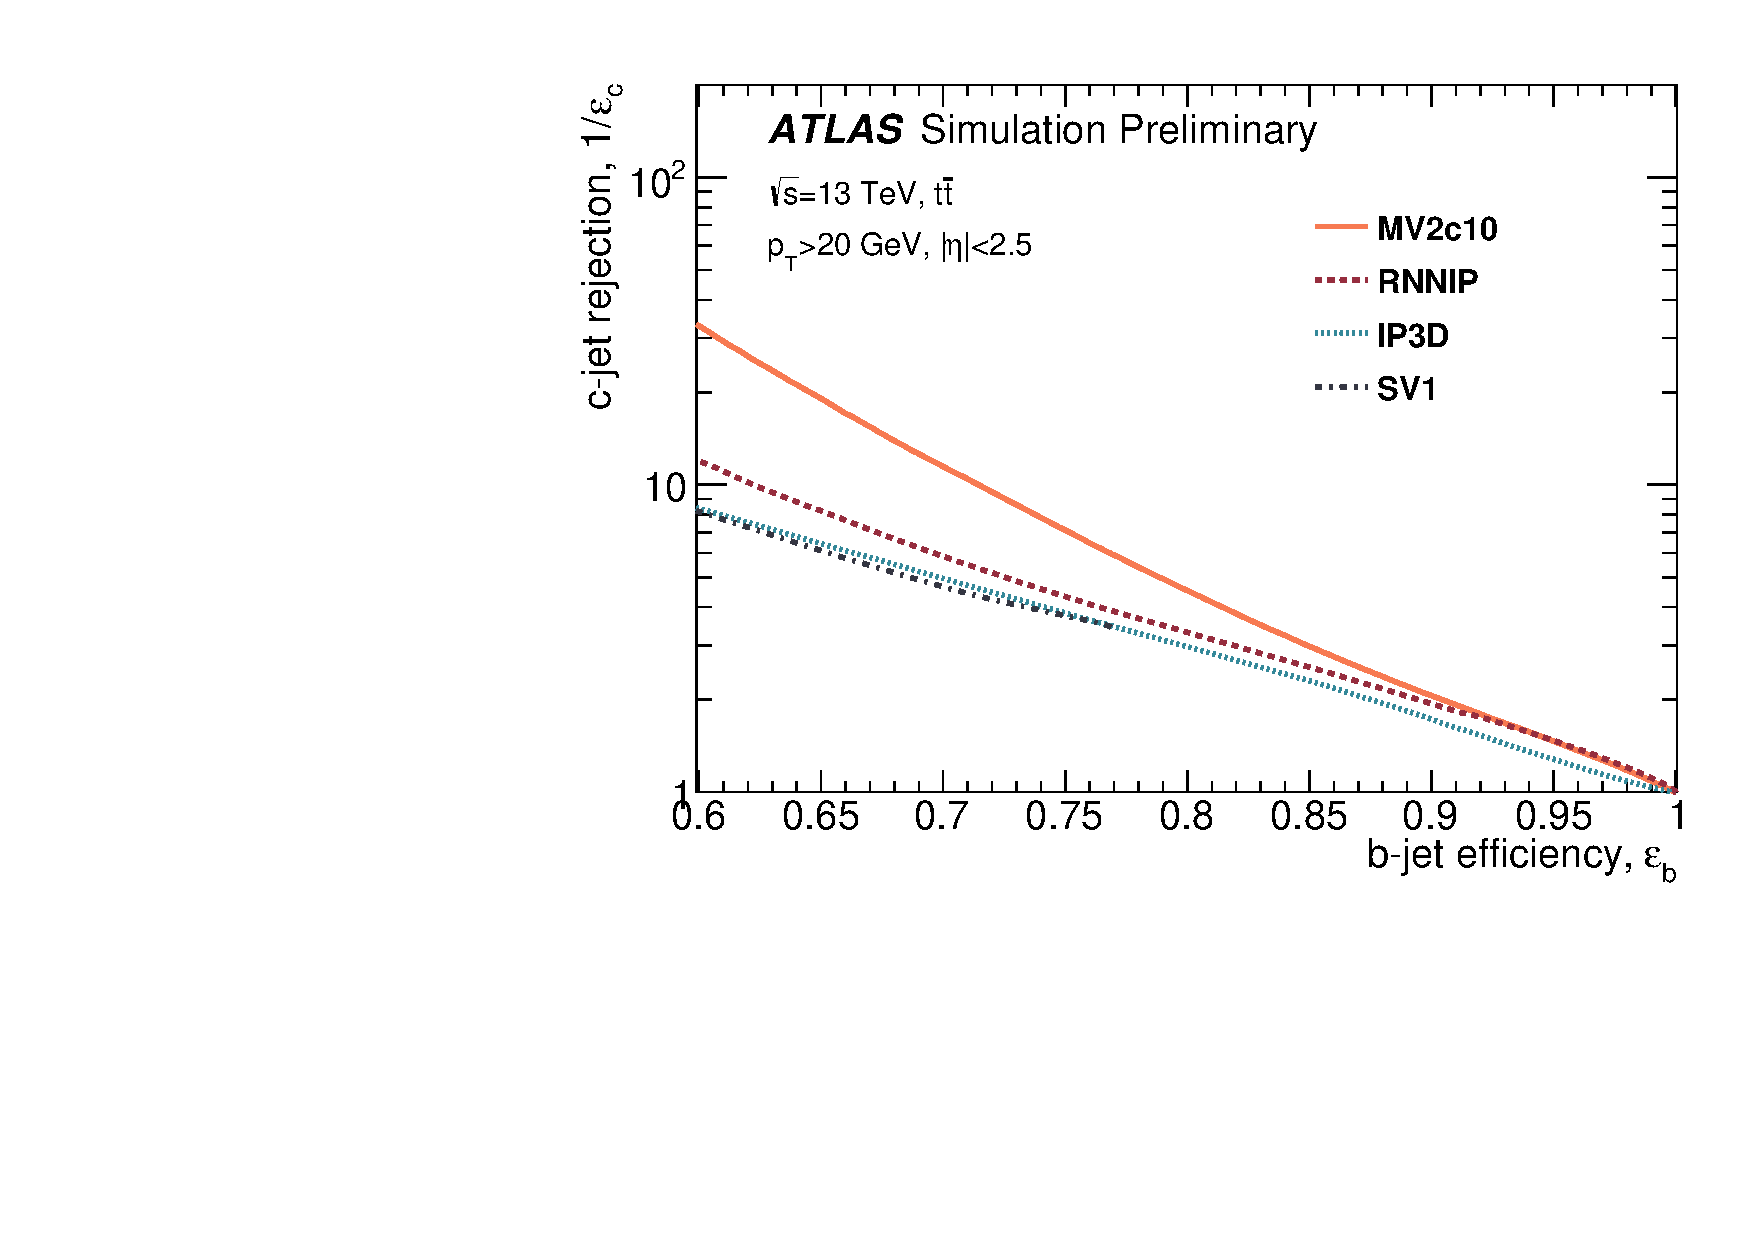
\includegraphics[width=0.48\linewidth]{\figpath/fig_03b}
    } 
    \caption{}
    \label{fig:\jetdef-fig3}
\end{figure}





%%%%%%%%%%%%%%%%%%%%%%%%%%%%%%
% VR track jets
%%%%%%%%%%%%%%%%%%%%%%%%%%%%%%

\FloatBarrier
\clearpage
\subsection{VR track jets optimization}

\hl{I had to have had a dR matching in this plot \ldots let's look up what it was!}

\begin{figure}[htbp]
  \centering
  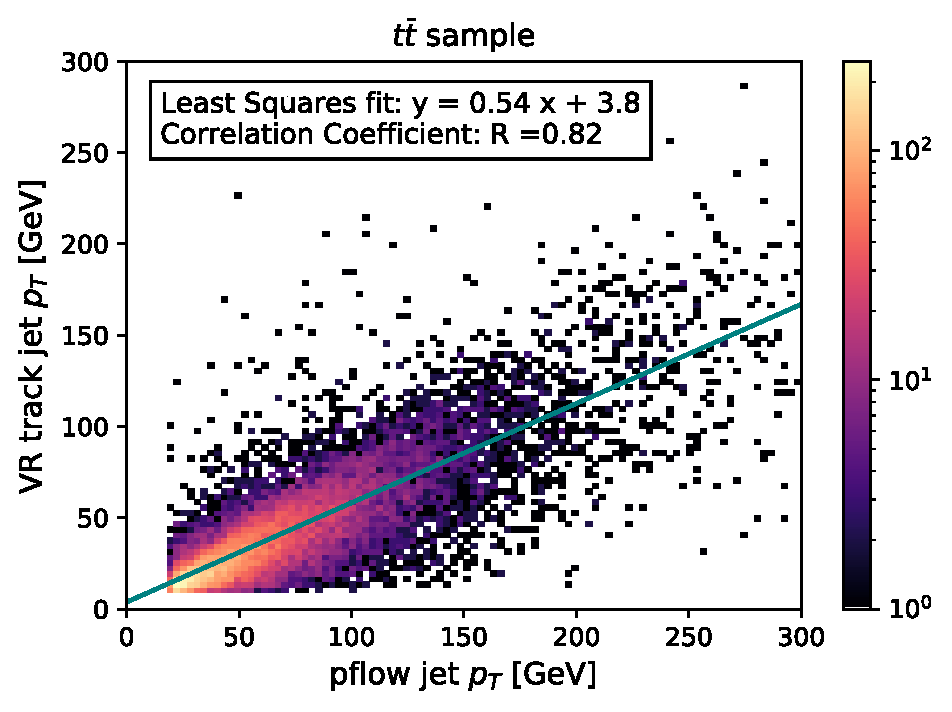
\includegraphics[width=.45\textwidth]{figures/ftag/VR trainings/pt-VR-pflow-ttvar}
  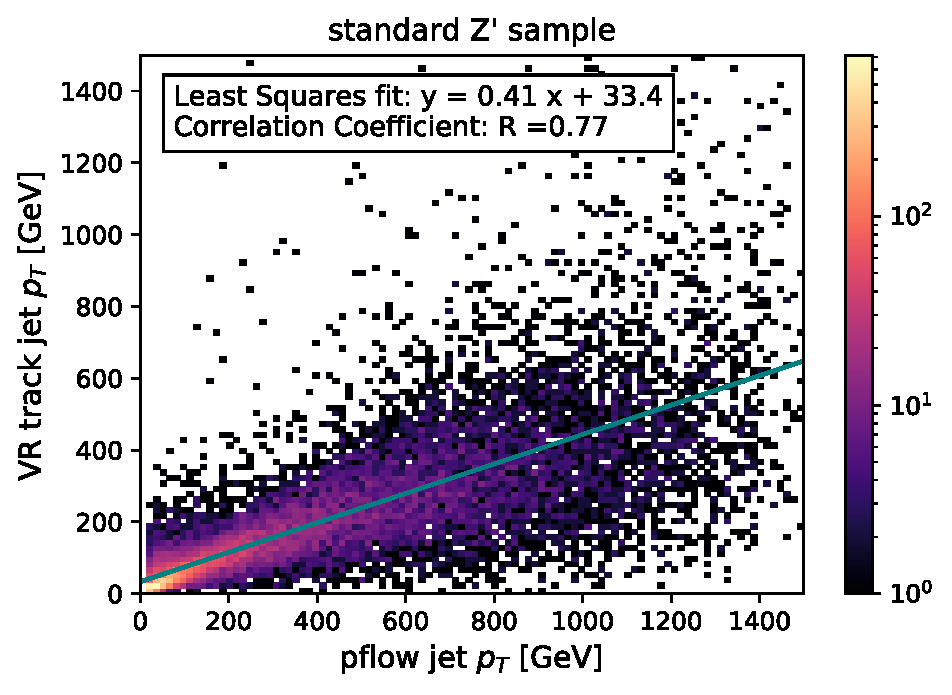
\includegraphics[width=.45\textwidth]{figures/ftag/VR trainings/pt-VR-pflow-std-Zprime}
  \caption{Comparison of the PFlow and VR track jet \pt for jet reconstruction.}
  \label{fig:pt-VR-pflow}
\end{figure}

Note: This plot \emph{motivated} us to move the pT cut on the light and c-jets to 125~GeV (although we kept the b-hadron \pt cut at 250 GeV).

\begin{figure}[htbp]
  \centering
  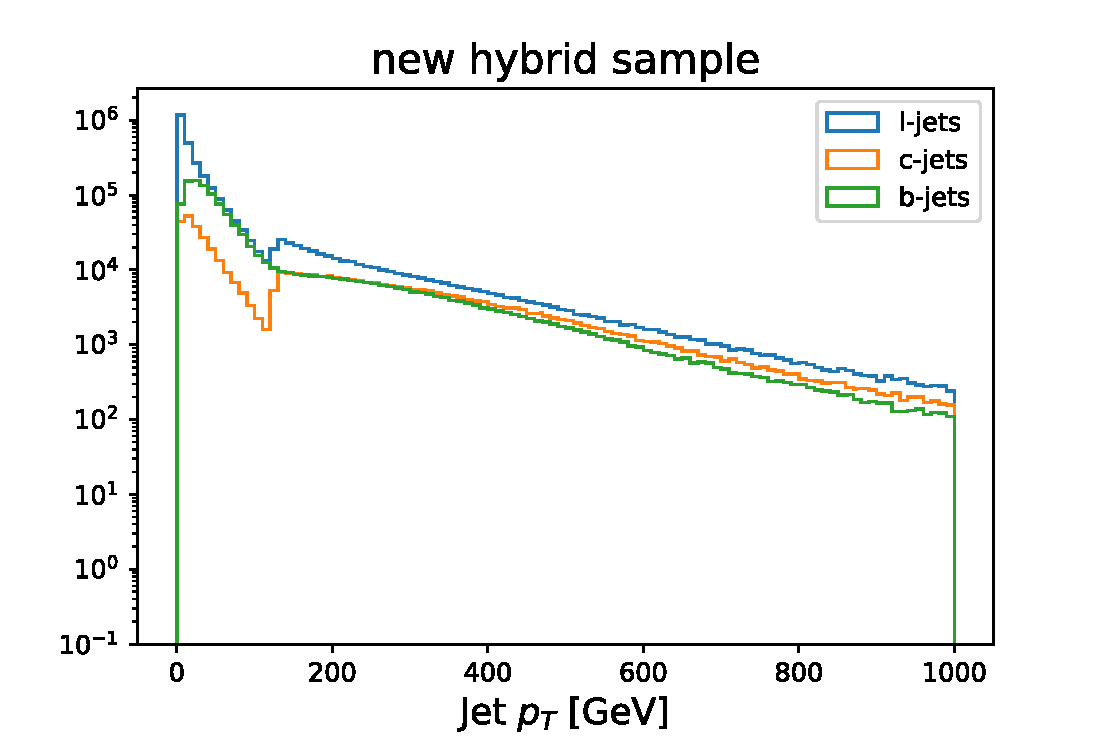
\includegraphics[width=.6\textwidth]{figures/ftag/VR trainings/pt-hyb-vr}
  \caption{The \pt spectrum for the VR track jets using the modified sample cut of 125~GeV for the light jet and \Pqb-jet \pt.}
  \label{fig:pflow-pt-extended-hybrid}
\end{figure}



\begin{figure}
\centering
\subfloat[light rejection]{
	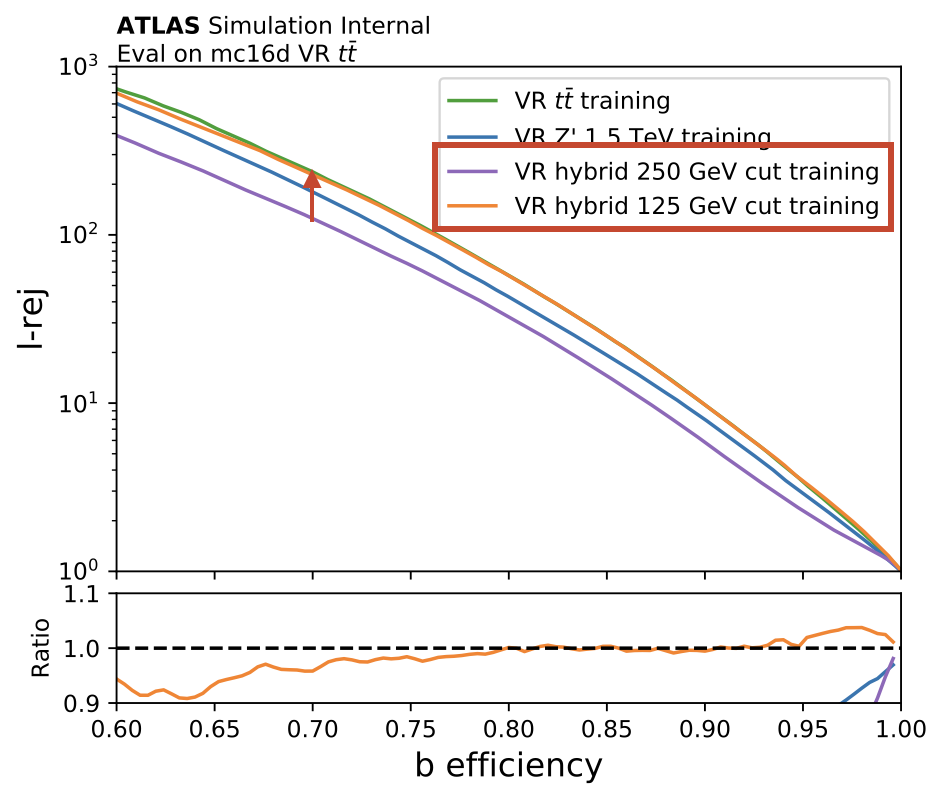
\includegraphics[width=0.45\textwidth]{{figures/ftag/VR\ Trainings/roc-new-cut-l-ttbar}}
	}
\subfloat[\Pqc rejection]{
	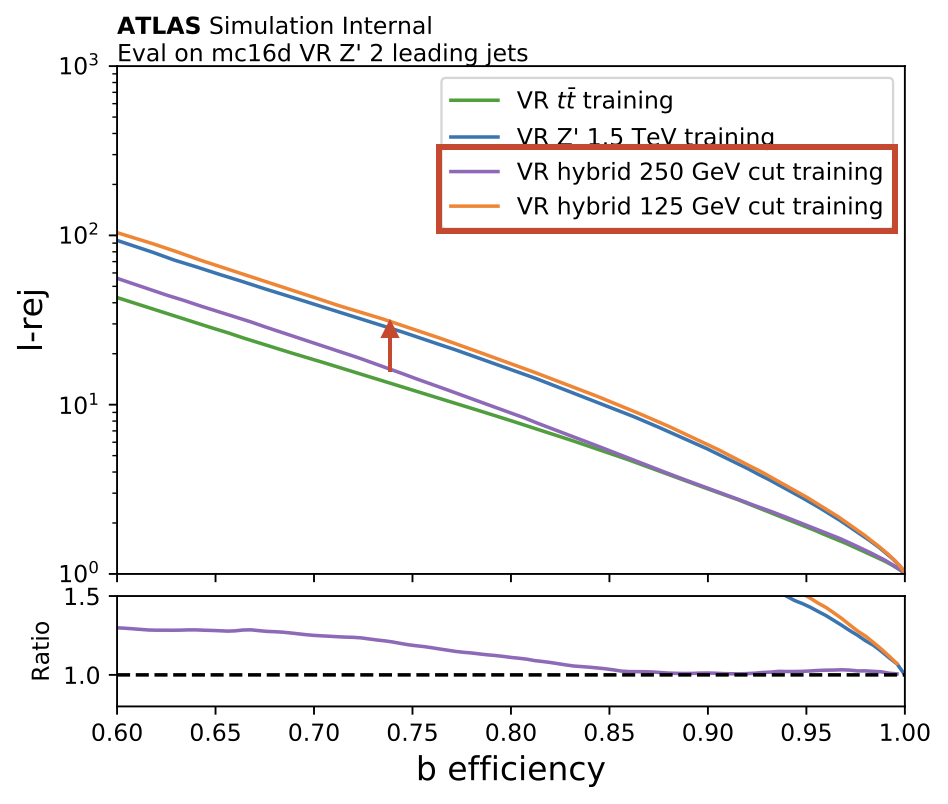
\includegraphics[width=0.45\textwidth]{{figures/ftag/VR\ Trainings/roc-new-cut-l-Zprime}}
	}
\caption{}
\label{fig:VR-improvements}
\end{figure}



\begin{figure}
\centering
\subfloat[light rejection]{
	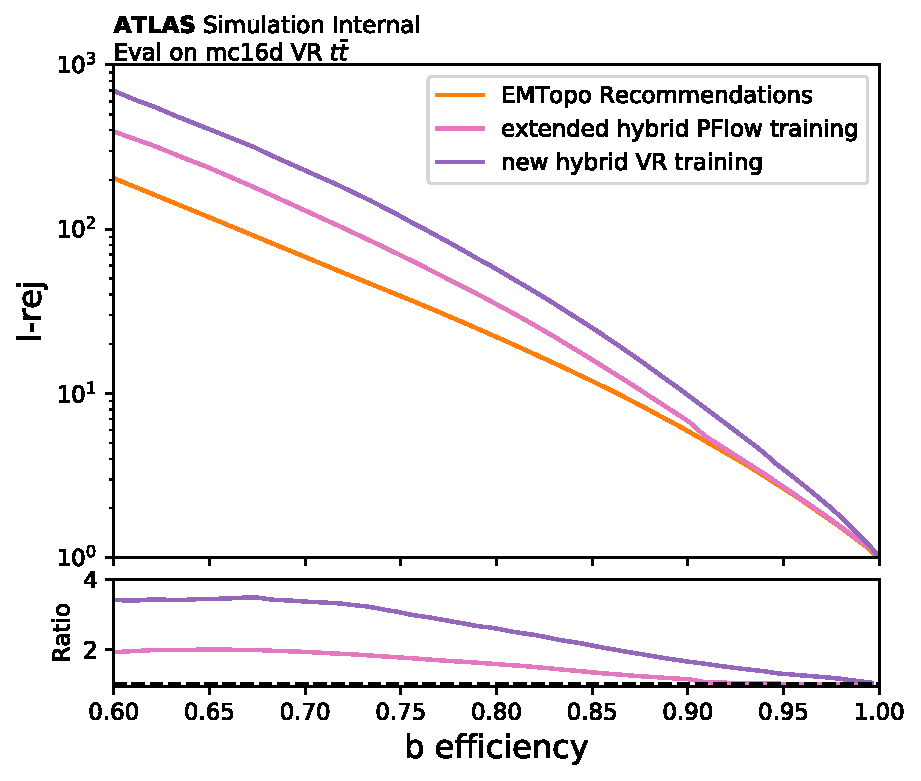
\includegraphics[width=0.45\textwidth]{{figures/ftag/VR\ Trainings/roc-vr-trainings-l}}
	}
\subfloat[\Pqc rejection]{
	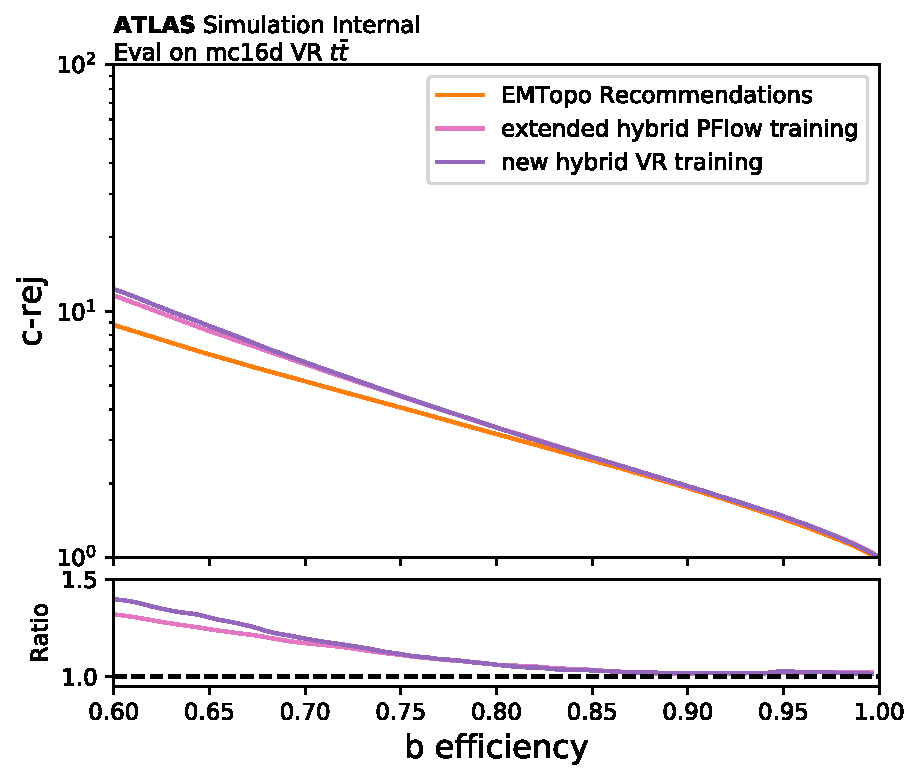
\includegraphics[width=0.45\textwidth]{{figures/ftag/VR\ Trainings/roc-vr-trainings-c}}
	}
\caption{}
\label{fig:VR-improvements}
\end{figure}

\begin{enumerate}
	\item \textcolor{orange}{EMTopo Rec: What we were applying to VR track jets now}
	\item \textcolor{deeppink}{Ext Pflow: If we applied the my new pflow training to VR track jets}
	\item \textcolor{mediumpurple}{New hybrid VR training: NEW dedicated VR training}
\end{enumerate}




\def\jetdef{VR}
% http://atlas.web.cern.ch/Atlas/GROUPS/PHYSICS/PLOTS/FTAG-2019-006/

\def\figpath{figures/ftag/\jetdef \ trainings}

\begin{figure}[htbp]
    \centering
    % light
    \subfloat[]{ 
            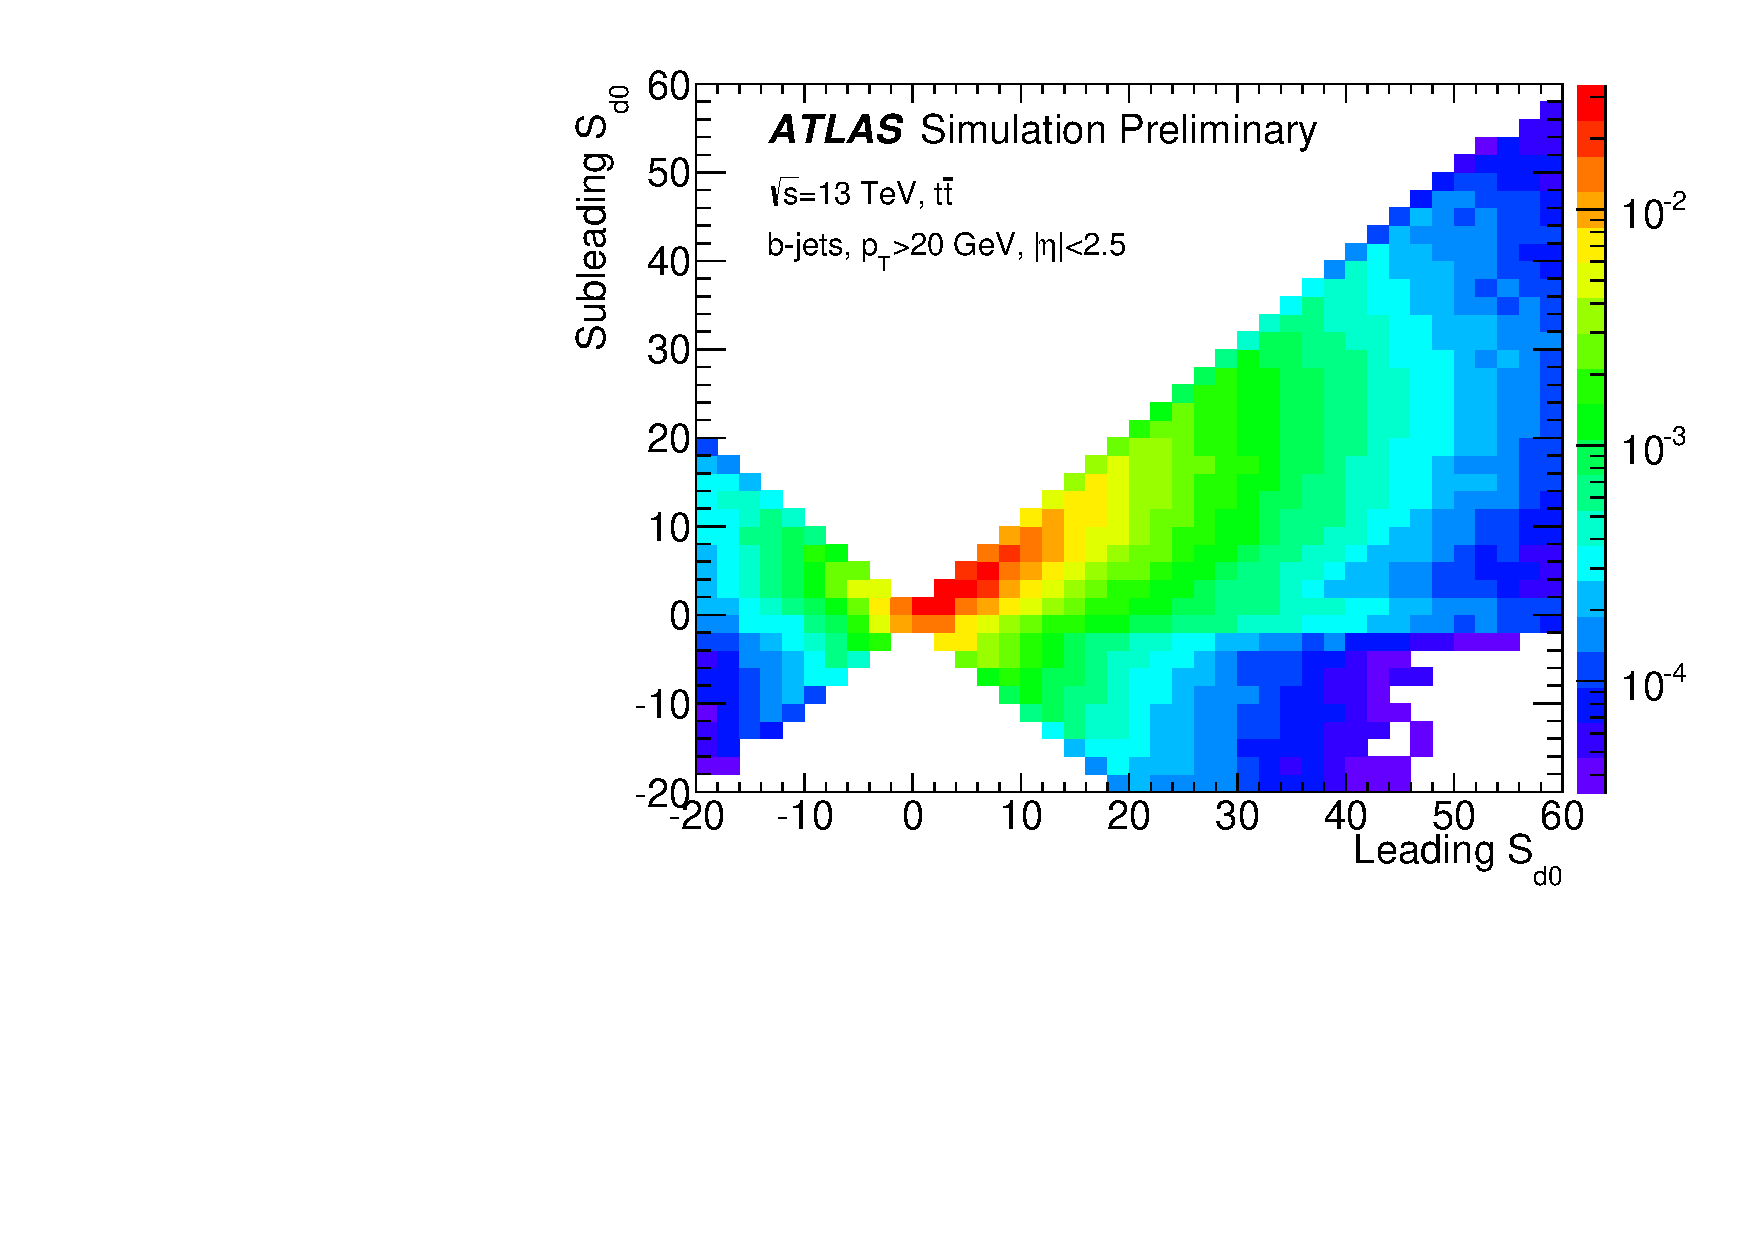
\includegraphics[width=0.48\linewidth]{\figpath/fig_01a}
    } 
     \subfloat[]{ 
            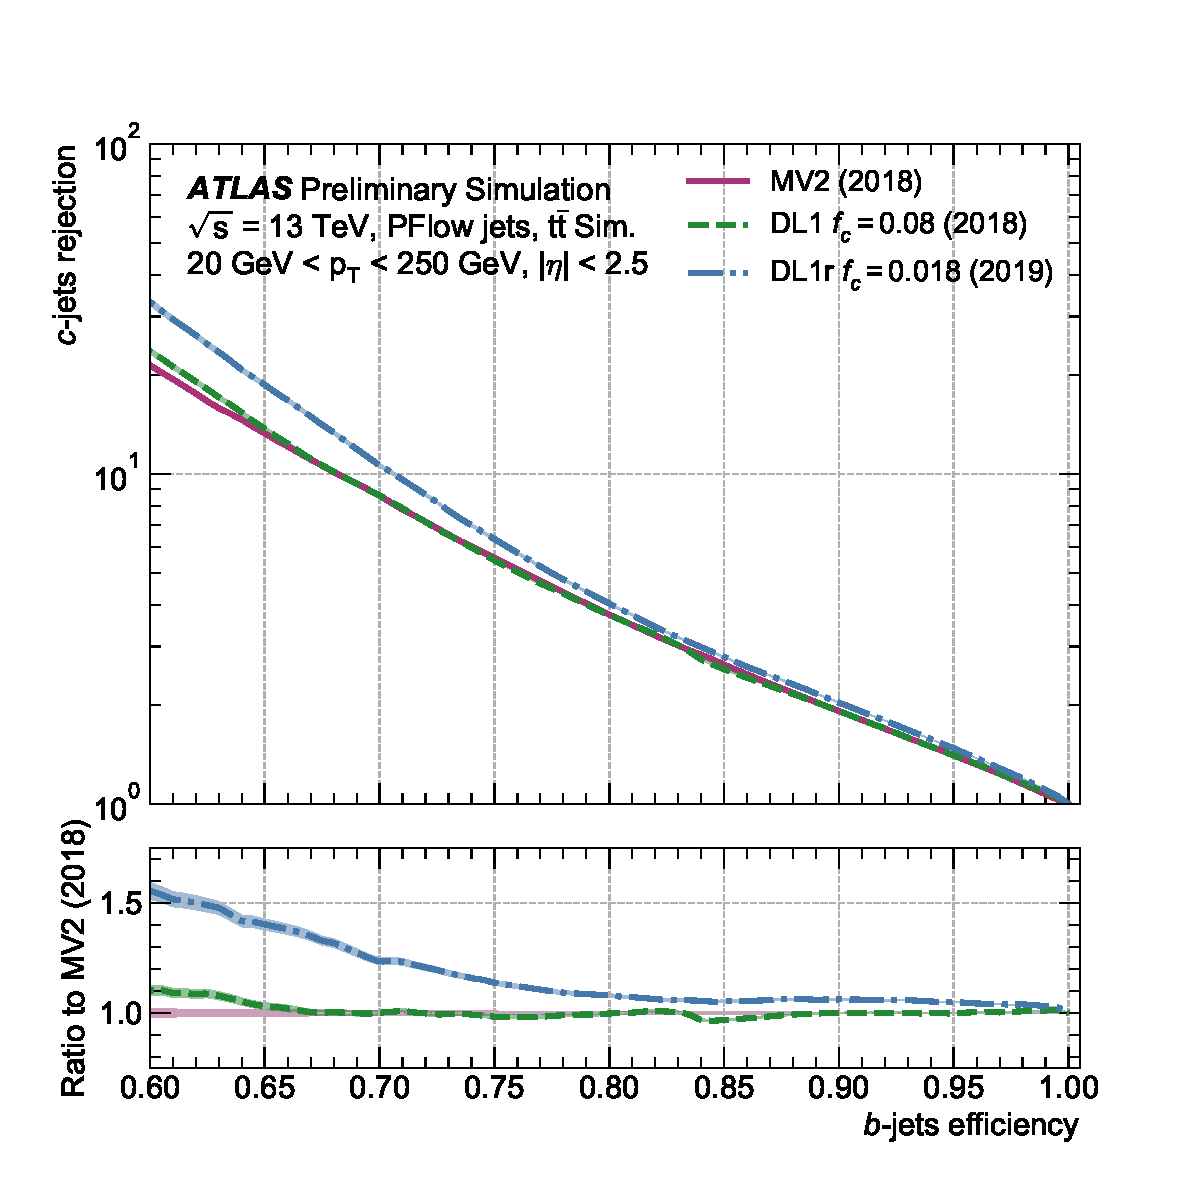
\includegraphics[width=0.48\linewidth]{\figpath/fig_01b}
    } 
    \caption{}
    \label{fig:\jetdef-fig1}
\end{figure}

\begin{figure}[htbp]
    \centering
    % light
    \subfloat[]{ 
            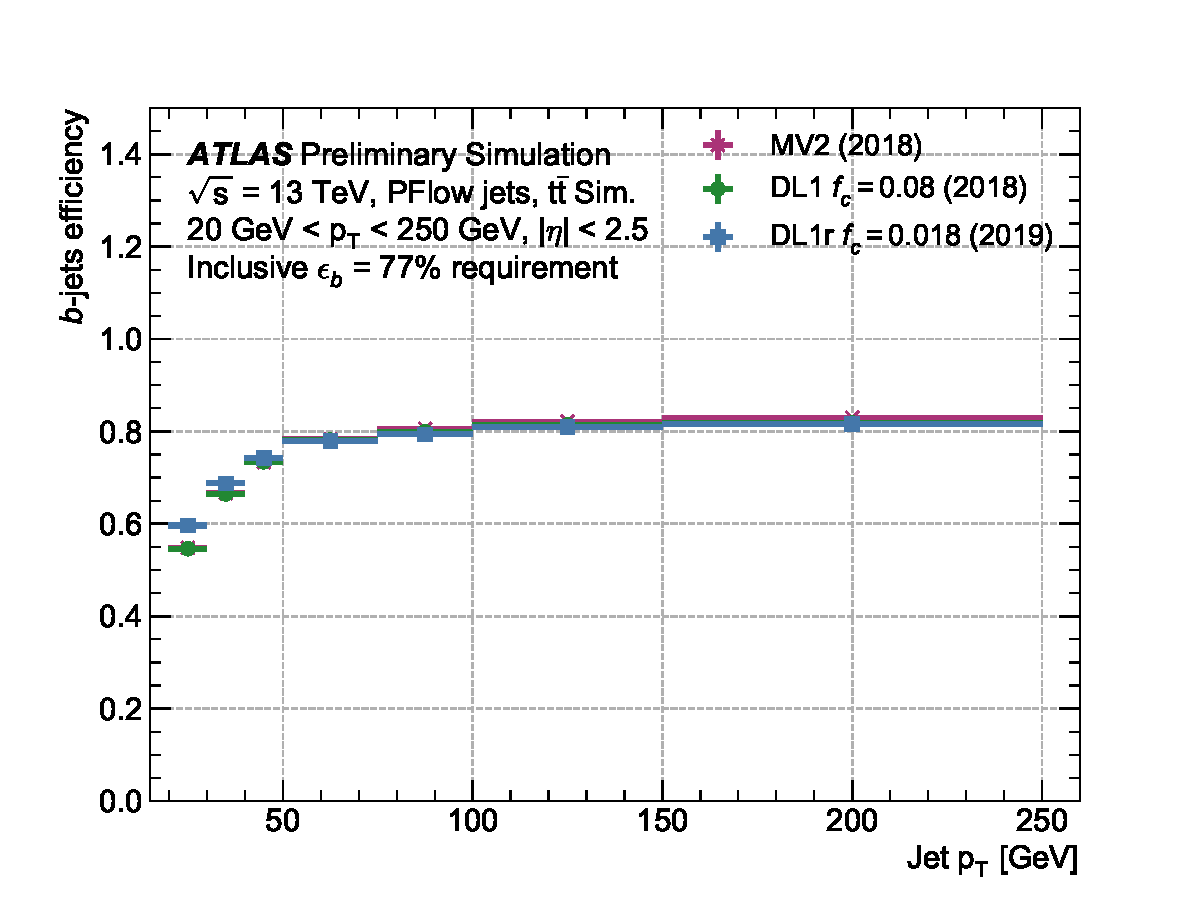
\includegraphics[width=0.33\linewidth]{\figpath/fig_02a}
    } 
     \subfloat[]{ 
            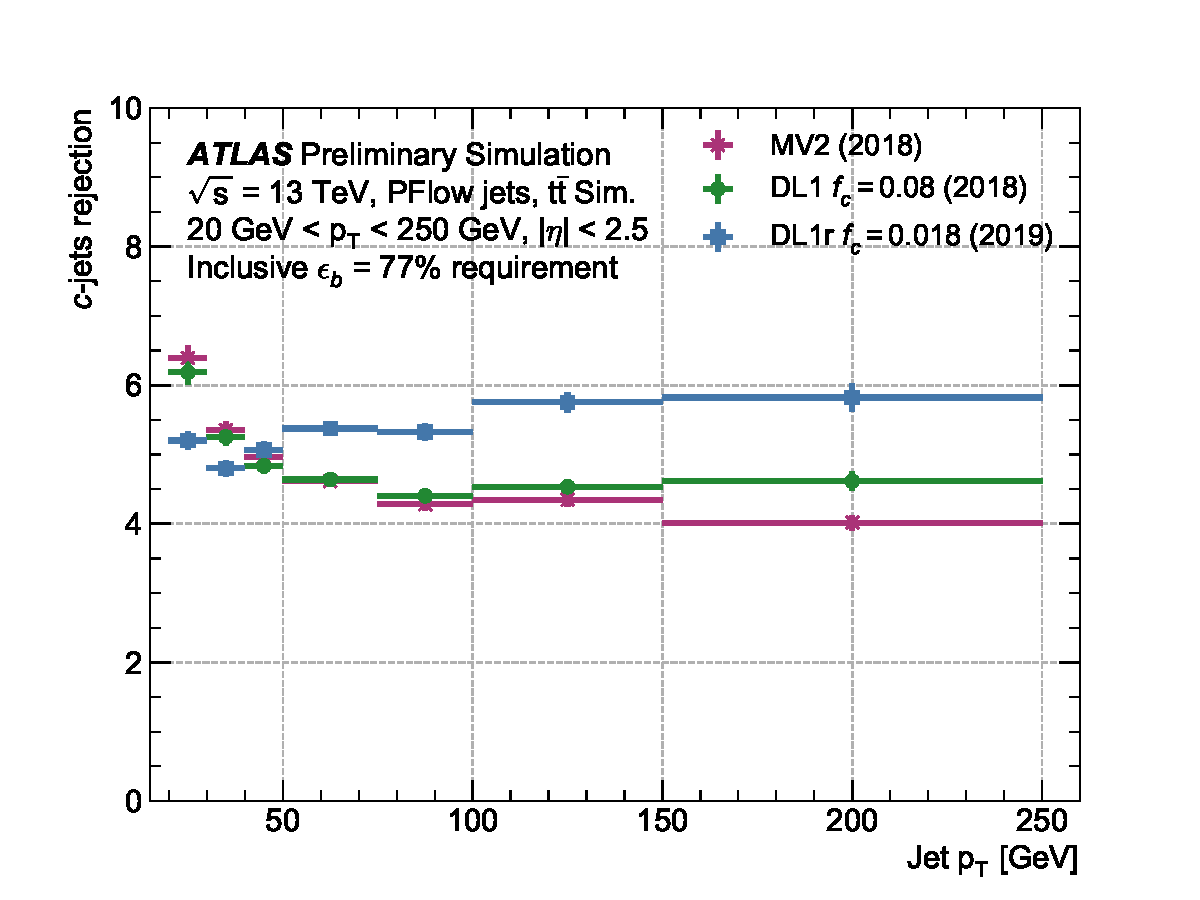
\includegraphics[width=0.33\linewidth]{\figpath/fig_02b}
    } 
    \subfloat[]{ 
            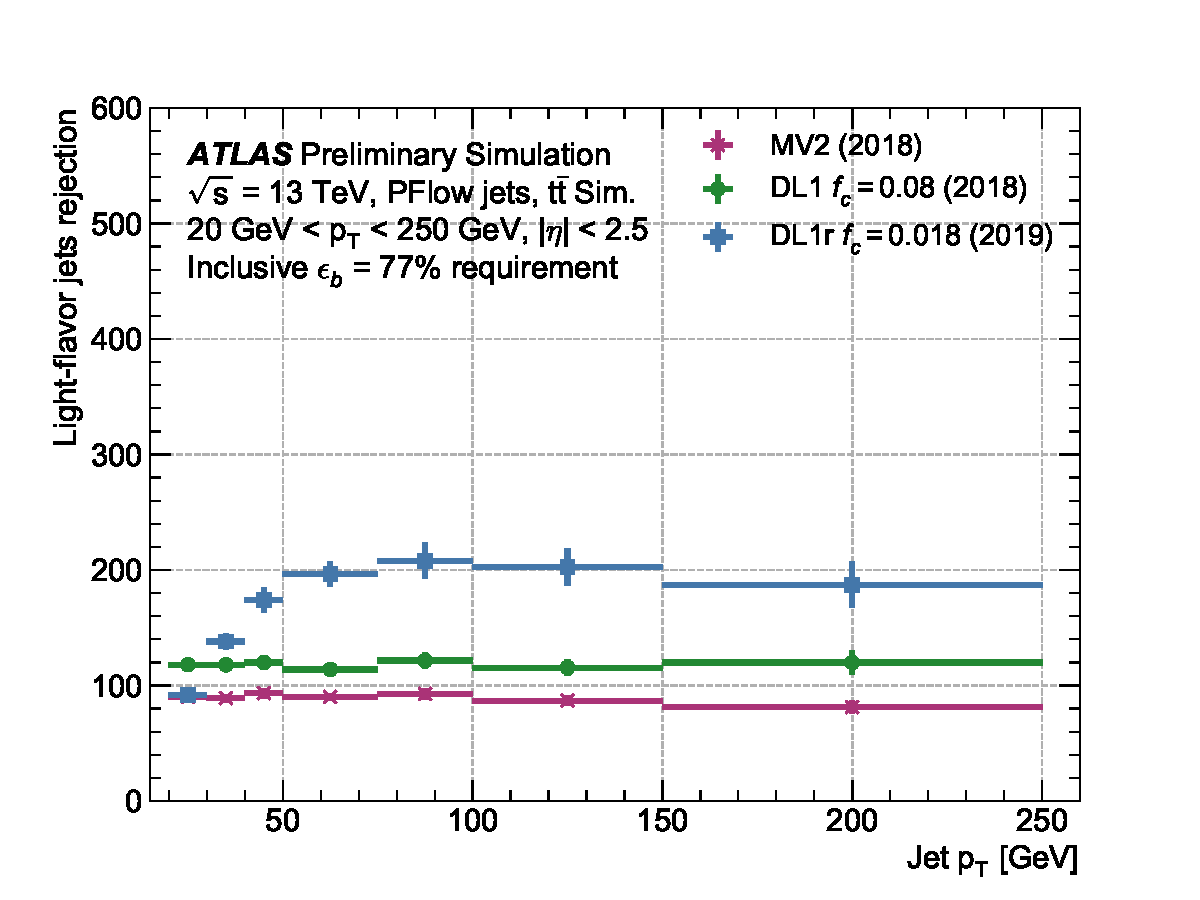
\includegraphics[width=0.33\linewidth]{\figpath/fig_02c}
    } 
    \caption{}
    \label{fig:\jetdef-fig2}
\end{figure}

\begin{figure}[htbp]
    \centering
    % light
    \subfloat[]{ 
            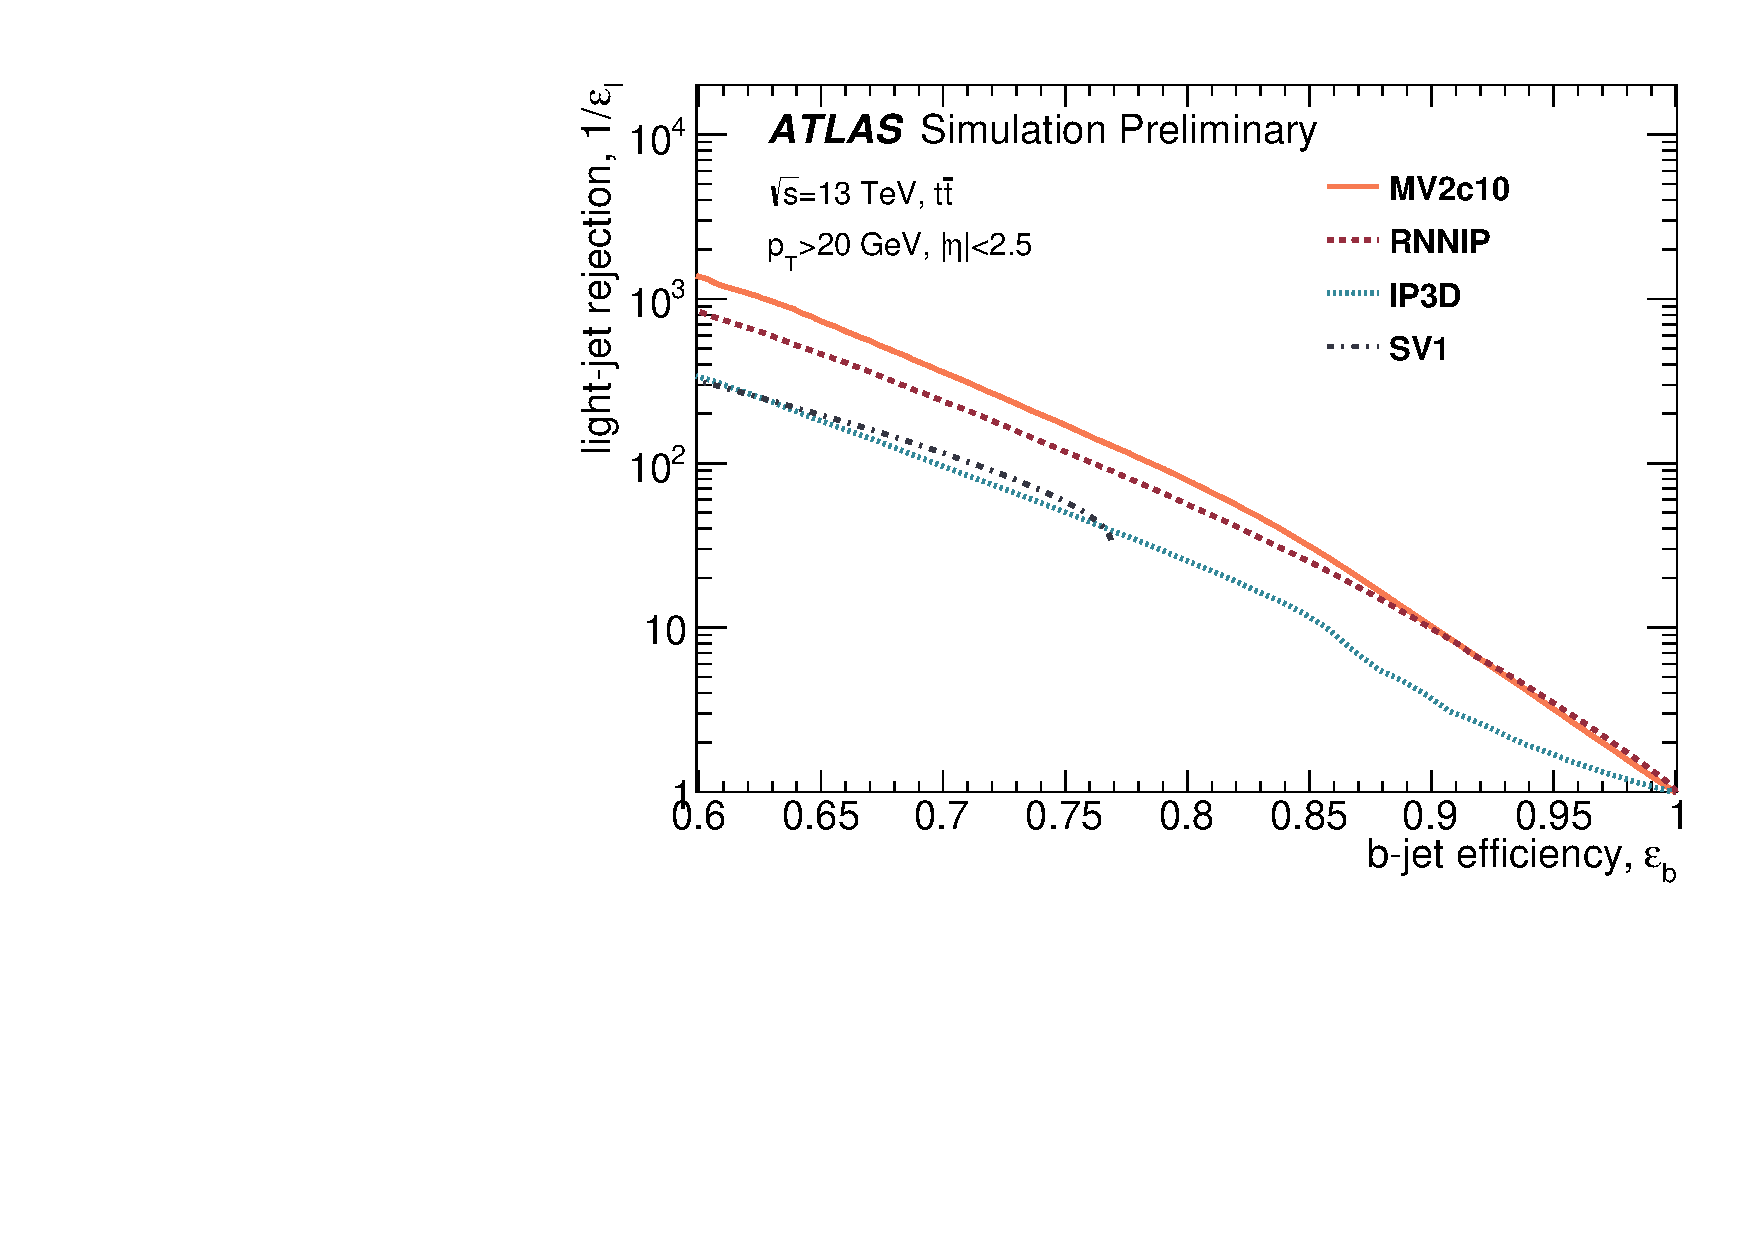
\includegraphics[width=0.48\linewidth]{\figpath/fig_03a}
    } 
     \subfloat[]{ 
            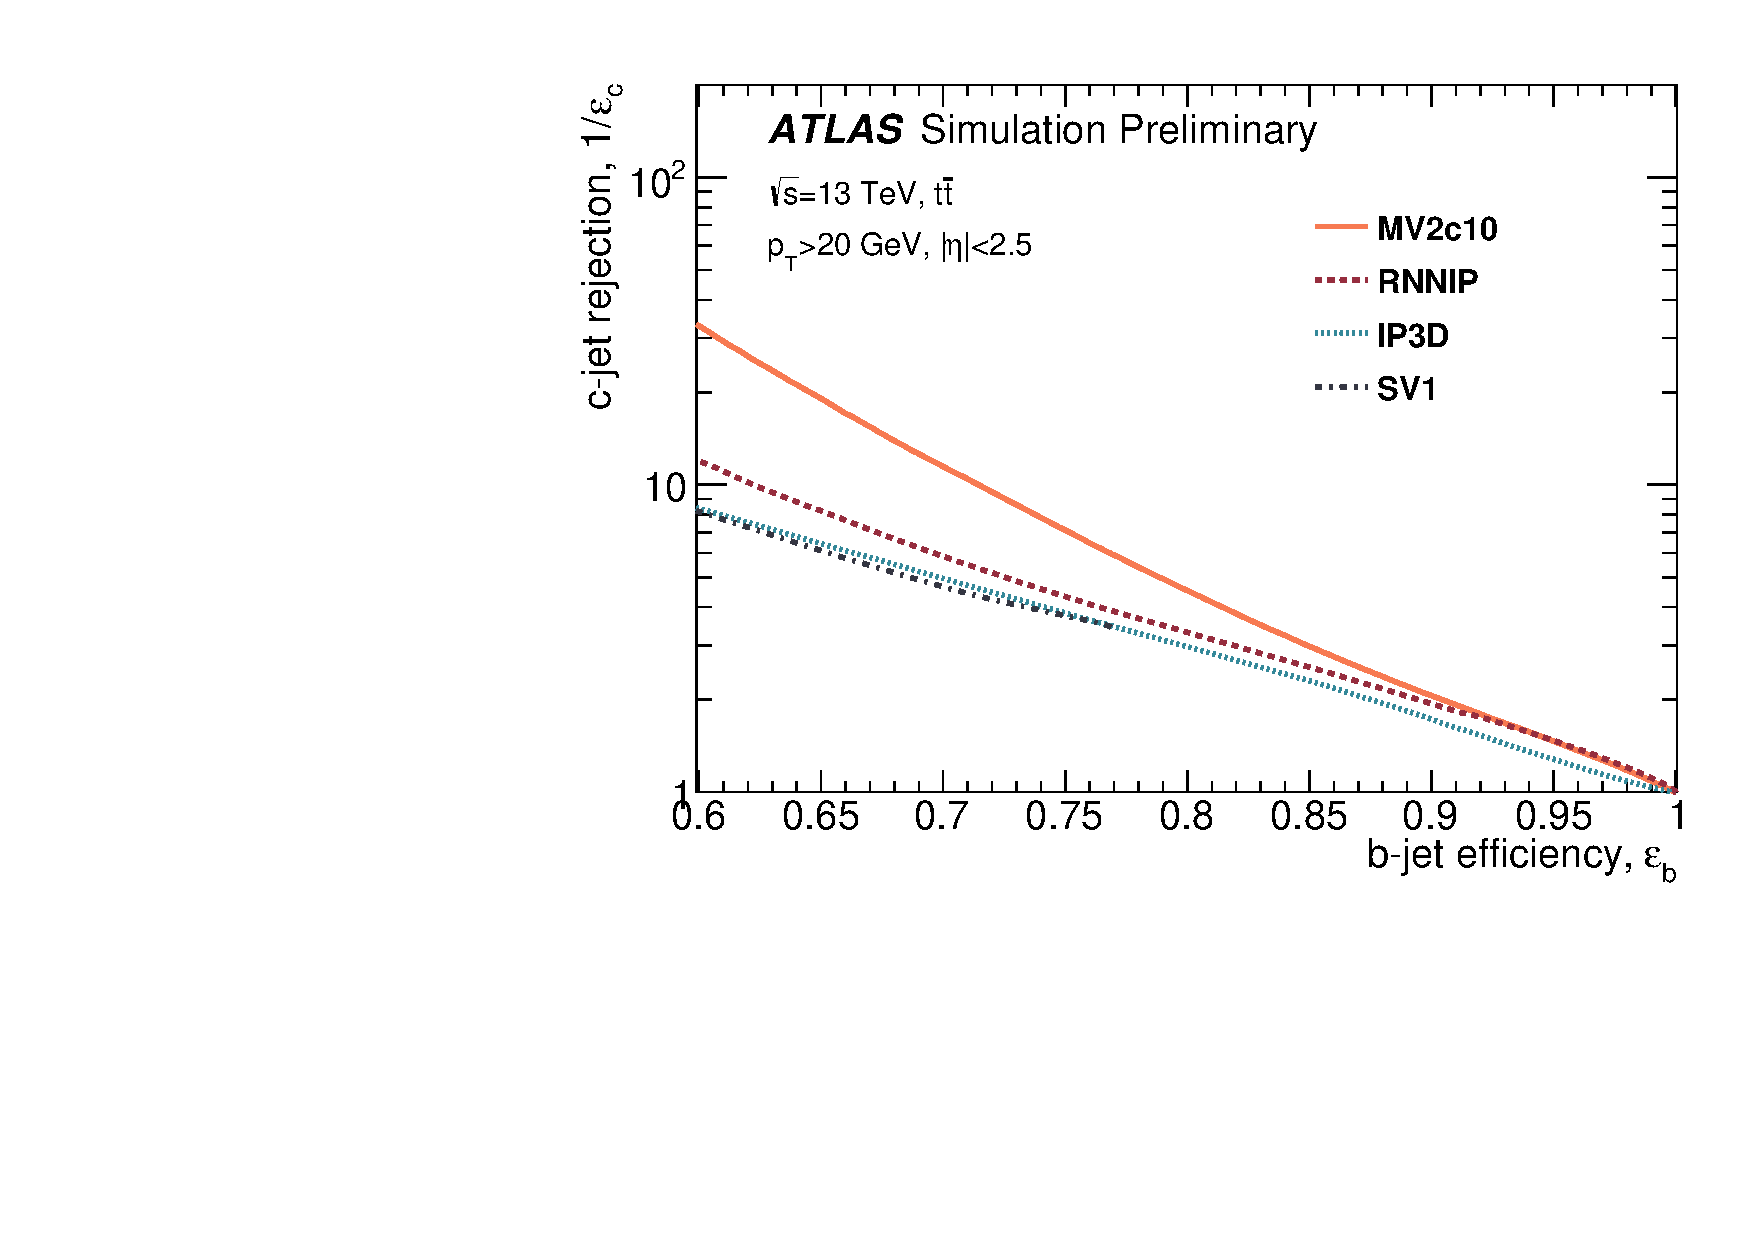
\includegraphics[width=0.48\linewidth]{\figpath/fig_03b}
    } 
    \caption{}
    \label{fig:\jetdef-fig3}
\end{figure}

\subsection{Impact of FTAG improvements on analyses}

\begin{figure}
\centering
\includegraphics[width=\textwidth]{figures/my_dihiggs/HH4b-boosted-vr-trk-jet-improvements.pdf}
\caption{Need to cite the 36 ifb and 139 ifb.}
\label{fig:boosted-vr-trk-jet-improvements}
\end{figure}


\section{RNNIP calibratability}



\section{Tagger R\&D: DIPS}

% DIPS intro (?) 

This work builds on that of the RNNIP algorithm \cite{ATL-PHYS-PUB-2017-003}, which uses impact parameter information and recurrent neural networks (RNNs) for $b$-tagging, and provides improvements over other IP-based algorithms by accounting for the correlations between the track features, and the inclusion of additional discriminating variables. % impact parameters.
tracks in the jet.
Here a new algorithm is introduced, Deep Impact Parameter Sets (DIPS), based on the Deep Sets architecture \cite{DBLP:journals/corr/ZaheerKRPSS17} and on the application of the Deep Sets formalism within particle physics known as Energy / Particle Flow Networks~\cite{Komiske_2019}.
DIPS solves the same task as RNNIP but treats the tracks in the jet as an unordered, variable-sized set rather than as a sequence, avoiding the need to specify a sequence ordering and the slow processing of RNNs. 
Given that the $b$-hadron decay products do not exhibit any intrinsic sequential ordering, the Deep Sets architecture is also better physically motivated.

DIPS is demonstrated to be as performant as RNNIP but faster to train, decreasing evaluation time and reducing turn-around time for optimization. Therefore, optimization studies of the track selection criteria and new track features are also included.
In addition, a discussion on how to measure the algorithm's efficiency in data, in particular for jets that do not contain a $b$ or a $c$-hadron, is presented. %light flavoured jetsone of the challenges for including machine learning algorithms in our existing workflows is the ability to calibrate them using our existing methods, especially the particularly challenging calibration of the light-quark initiated jet mistag rate, and thus we demonstrate that DIPS is well suited to standard calibration procedures.
Finally, one avenue of research in deep learning models is exploring the interpretability of the models, or trying to dissect what information the network is learning. 
Diagnostic studies from the machine learning literature are presented to demonstrate the well-known characteristics from $b$-quark fragmentation and hadronization process that the network has gleaned.


% --------
% This info can go in the algorithm description part:
% The Deep-Sets implementation, which we denote DIPS (Deep Impact Parameter Sets), exploits a hierarchical organization of the information inside of the jet through separate networks that first operate on the tracks and extract track features and then operate on the jets to take into account correlations with high-level features, but can be trained together end-to-end. 
% --------



\def\figpath{figures/ftag/dips-note/}

\subsection{Algorithm overview}

The Deep Sets architecture~\cite{DBLP:journals/corr/ZaheerKRPSS17}, which treats the elements as a set without any specific order, maintains the benefits of the RNNIP algorithm, while avoiding the required element ordering (which for $b$-tagging is empirically driven rather than strictly dictated by the inputs of the problem).
This architecture was first employed in particle physics in a phenomenological study on the identification of different types of jets~\cite{Komiske_2019}.  
Adopting the formalism of \cite{Komiske_2019}, if $p_i$ is the vector representing the inputs associated with the $i^{th}$ track in the jet, then the Deep Sets architecture applies a neural network (NN) $\Phi$ to each track, sums over the tracks, and then applies additional processing on the summed representation with a feed forward NN $F$, as described in equation~\ref{eq:DeepSets},

\begin{equation}
\mathcal{O}\left(  \{ p_1 , \ldots , p_n \}  \right) = F \left( \sum_{i = 1}^n \Phi \left( p_i \right) \right),
\label{eq:DeepSets}
\end{equation}

where $\mathcal{O} \left(  \{ p_1 , \ldots , p_n \}  \right)$ represents the $b$-, $c$-, and light-flavour class probabilities derived from the inputs for the $n$ tracks in the jet. 
The architecture bifurcates the problem into operations over inputs and operations over sets, where the track-network $\Phi$ extracts the relevant track features, and the jet-network $F$ accounts for the correlations between the tracks. 
The permutation invariance of the set is encoded with the permutation invariant sum operation, although other permutation invariant operations such as the max or average could be used as well. 
The presence of this aggregation layer in the architecture encodes information about track multiplicity inside the jet, which is a useful information for identifying $b$-jets.

This Deep Sets architecture offers the same advantages as RNNIP but encodes permutation invariance between the tracks in the jet, giving a more natural representation of the data and allowing the algorithm to be trained more efficiently with fewer parameters and less data \cite{DBLP:journals/corr/abs-1806-01261}.  
In addition, Deep Sets offers a major additional advantage over RNNs in that the operation of processing the tracks in the jet with the $\Phi$ network can be easily parallelised. 
This allows training and evaluation to make significantly more efficient use of GPUs over the non-parallelisable iterative processing of the RNN. 
The timing performance comparison between DIPS and RNNIP is further discussed in Section \ref{subsec:timing}.
 
\subsection{Implementation details} 
\label{subsec:algdetails}


In this section, algorithms are just trained on $t\bar{t}$ simulated events (described in Section~\ref{sec:datasets}) for multi-class classification between $b$-jets, $c$-jets and light-flavour jets, with the \Pqb and \Pqc-jet distributions reweighted into the light jet distribution. 

For the timing comparisons in Section~\ref{subsec:timing}, the same input features are used for both RNNIP and the DIPS. 
% Additional input features are included for the Optimised DIPS algorithm, described in Section~\ref{subsec:optimisation}. 
The features used in each algorithm are described in Table~\ref{table:inputs}.
The track variables related to the track reconstruction quality focus on the IBL and the next-to-innermost pixel layer (PIX1) due to their strong impact on the IP significance distributions. 
In particular, the number of split hits, which are hits being created by multiple charged particles \cite{PERF-2012-05}, is used to help identify dense tracking environments, in which distinguishing tracks from  heavy flavour decays is generally  more difficult. 
% because these are most crucial for the $b$-tagging performance. 
% The track IP error is highly dependent on whether the track has hits in these first layers and thus impacts the IP significance distributions.

%using the track significances with respect to the PV, some variables characterizing the track kinematics $\pT^{frac} = $ and $\Delta R$ between the track and the (uncalibrated) jet axis, and 9 variables characterizing the hit quality of the track \textbf{list variables}.
%The direct use of the hit information instead of the category from IPXD is a new from \cite{ATL-PHYS-PUB-2017-003} but was what was done for \cite{PFlowPublicPlots2019} which is why this is the RNNIP implementation that we are comparing to. This switch to the hit level information gave a $\mathcal{O}(10\%)$ improvement (keeping everything else in the training setup constant).

After applying the track selections described in Section~\ref{sec:datasets}, the tracks are ordered by decreasing $s_{d0}$, and the first 15 tracks are kept for processing. 
The ordering plays a limited role in the algorithm, since typical jets in the topology investigated should have an average number of tracks that is smaller than the maximum allowed number of tracks (see Table~\ref{table:trkComposition}).
% The number of tracks considered is a trade-off between model complexity, with training and evaluation time growing with this requirement, and algorithm performance.
% for the nominal track selection, while 25 tracks are kept with the looser track selection. 
Since the $\pT^{frac}$ and $\Delta R$ variables have a tail at larger values, the natural log of the value for these variables is used as the feature in order to improve the convergence time of the training.  
Variable normalisation to zero mean and unit variance is frequently used for preprocessing of features in ML algorithms. 
As many of our input variables already have near zero mean, only a subset of the track features are normalised: $\log \pT^{frac}$, $\log \Delta R$, nPixHits, nSCTHits, as well as $d_0$ and $z_0 \sin \theta$ for the optimised DIPS training.

A simplified scheme of the DIPS architecture is shown in Figure~\ref{fig:architecture}, which is based on the architecture in reference~\cite{Komiske_2019}.  
A grid search over the hyperparameters including the number of layers in the $\Phi$ and $F$ networks, the number of nodes in the $\Phi$ and $F$ networks and the dimension of the track latent space revealed similar performance for many different choices of these hyperparameters. 
Both batch normalisation \cite{DBLP:journals/corr/IoffeS15} and dropout \cite{DBLP:journals/corr/abs-1207-0580} were tested, and it was found that batch normalisation was helpful for the DIPS $b$-tagging performance while dropout was not.

\begin{figure}
  \centering
  \includegraphics[width=0.8\linewidth]{\figpath/DIPS_architecture}
  \caption{Architecture for the DIPS algorithm. The number of hidden units in the different neural network layers correspond to the final optimized architecture.}
  \label{fig:architecture}
\end{figure}

We present a different training for RNNIP than \cite{ATL-PHYS-PUB-2017-003} and \cite{PFlowPublicPlots2019}, here training on only $t\bar{t}$ for the timing comparisons. RNNIP processes the inputs using an LSTM cell with 100 hidden units, and after processing the sequence, feeds the vector into a feedforward network with 20 units and a dropout fraction of 0.2 before a softmax layer for classification. 

The RNNIP and DIPS trainings were performed with 3 million jets, with 20\% of these jets held out as a validation set to determine when to stop the training. 
After 10 consecutive training epochs (or iterations through the training dataset) without finding a new validation loss minimum, the training is terminated and the model with the best validation loss was selected.  Both the RNNIP and DIPS architectures were implemented in Keras \cite{chollet2015keras} and trained with the TensorFlow backend \cite{tensorflow2015-whitepaper}. 
Algorithms were trained with the Adam optimizer \cite{kingma2014adam} with a learning rate of $10^{-3}$ and a batch size of 256. 
The performance metrics shown in the following sections are obtained with a statistically independent dataset of 3 million jets.

\subsection{Performance}

\subsection{Baseline Performance}
\label{subsec:baseline}

The distribution of the DIPS discriminant $D_b$ (defined in Equation~\ref{eq:dipsdiscriminant}) for each of the jet flavours is shown in Figure~\ref{fig:Db}. 
The peak at $D_b = -1.3$ is due to jets without any selected tracks. 
Clear separation between the distribution of $b$-jets and light-flavour jets can be seen, as well as a strong but smaller separation between $b$-jet and $c$-jets as expected due the similarities between $b$-hadron and $c$-hadron decays.

\begin{figure}[h!]
  \centering
  \includegraphics[width=0.5\linewidth]{\figpath/disc_DIPS_phi_100_100_128_F_100_100_3out_bn_3mtrain_15trks_sd0_sz0_nNextToInnHits_nInnHits_nsharedBLHits_nsplitBLHits_nsharedPixHits_nsplitPixHits_nsharedSCTHits_logNorm_ptfrac_dr_norm_nPixHits_nSCTHits_iter1}
  \caption{Distributions of DIPS $b$-tagging discriminant, as defined in Equation \ref{eq:dipsdiscriminant}, for $b$-jets, $c$-jets and light-flavour jets.}
  \label{fig:Db}
\end{figure}

The performance of taggers can be examined and compared through a Receiver Operator Characteristic (ROC) curve: a scan is performed for a threshold $\tau$ on $D_b$, and the efficiency for $b$-jets at each threshold is computed as the fraction of $b$-jets with $D_b > \tau$, while the rejection of $c$-jets or light-flavour jets is computed as one over the fraction of $c$-jets or light-flavour jets (inverse mistag efficiency), respectively, with $D_b > \tau$. 
The $b$-jet efficiency and light-flavour (or $c$) jet rejection for the same $\tau$ are then plotted.  Each model is trained five times and for a given $b$-jet efficiency, the mean of the rejections is used as the nominal value and the standard deviation of the rejections is used for the width of the curve. 
This ensemble of trainings is known to assess the predictive uncertainty of machine learning-based algorithms~\cite{deepensembles}.

The ROC curves for $b$-jet efficiency versus light-flavour jet rejection and for $b$-jet efficiency versus $c$-jet rejection of the DIPS and RNNIP algorithms are shown in Figure~\ref{fig:roc_rnnip_dips}. 
% The width of the curves is calculated by repeating the algorithm training five times with different random weights
The lowest $b$-jet efficiency displayed corresponds to the lowest efficiency benchmark used in physics analyses within the ATLAS experiment. 
%, and Figure~\ref{fig:roc_rnnip_dips} also includes the Optimised DIPS discussed in Section~\ref{subsec:optimisation}. 
The DIPS algorithm provides up to a 15\% additional light-flavour jet rejection and a 5\% additional $c$-jet rejection at a given $b$-jet efficiency over the RNNIP algorithm. 
Notably, as will be discussed in Section~\ref{subsec:timing}, this similar performance comes with a significant decrease in training and evaluation time.

\begin{figure}[ht]
    \centering
    \subfloat[]{ 
            \includegraphics[width=0.48\textwidth]{\figpath/rocAvgIter_l_rnnip_dips}
    }   
    \subfloat[]{ 
            \includegraphics[width=0.48\textwidth]{\figpath/rocAvgIter_c_rnnip_dips}
    }   
    \caption{Light-flavour jet rejection as a function of $b$-jet efficiency (a) and $c$-jet rejection as a function $b$-jet efficiency (b) of the RNNIP (green) and DIPS (purple) algorithms. The central curves and error bands show the mean and standard deviation, respectively, of the rejection at each $b$-jet efficiency for 5 trainings. The ratios are computed with respect to the RNNIP ROC curve.}
    \label{fig:roc_rnnip_dips}
\end{figure}

In order to explore what DIPS is learning in the correlations between features that aids the classification performance, the average saliency map for $b$-jets with 8 associated tracks and failing a threshold corresponding to 77\% $b$-tagging efficiency is shown in Figure~\ref{fig:saliency}. 
The saliency map is computed as 
\begin{equation}
\frac{\partial D_b}{\partial x_{ik}} = \frac{1}{N} \sum_{j=1}^N \frac{\partial D_b^{(j)}}{\partial x_{ik}^{(j)}}, 
\label{eq:salmap}
\end{equation}
and is the gradient of the discriminant value $D_b^{(j)}$ with respect to each track feature input $x_{ik}^{(j)}$, averaged over jets ($j$) in a sample of N jets~\cite{simonyan2013deep}.  
In this case, the feature inputs are normalized to zero mean and unit variance, in a similar way to the training procedure. 
The saliency map gives a linearised view of how the discriminant value is sensitive to changes in the inputs. Figure~\ref{fig:saliency} thus shows how  this sample of $b$-jets which failed tagging could be modified to make them more $b$-jet like.
One can see there is a reasonably strong positive gradients for the significances ($s_{d0}$ and $s_{z0}$) extending up to 5 tracks, which is the average number of charged particle tracks in a $b$-hadron decay. 
Beyond 5 tracks, the gradients for all features are either nearly zero or negative, indicating that either these tracks provide no further information or that tracks with large feature values are more indicative of background. 
In addition, DIPS is highly sensitive to the $\log \pT^{frac}$ and $\log \Delta R$ of the leading $s_{d_0}$ track, which is consistent with the harder fragmentation of $b$-quarks with respect to light-flavour and charm jets. Interestingly, this strong correlation with $\log \pT^{frac}$ and $\log \Delta R$ for the highest $s_{d_0}$ track also indicates that simply enlarging the IPs of a track in a jet would not directly lead to a jet passing a tagging threshold, as the track must also be consistent with the kinematic expectations from $b$-jet fragmentation.
The gradients for the shared and split hits of the high $s_{d0}$ tracks are strongly negative since tracks formed from random combinations of hits are more likely in highly dense environments.
It can also be seen that the correlation with the overall number of hits in the inner most pixel layers, IBL and PIX1, is positive but small. Such features are of high importance to the estimate of the IP and IP resolution. However such information is also encapsulated in the IP significance features which are strongly correlated with the discriminant. 
We suspect these correlations are observed to be relatively small due to the discriminator heavily relying on the IP significance for the first order estimate of the quality of the track and the track's utility for classification.
%indicating that we want the high $s_{d0}$ tracks to have good quality so that they are less likely to have been constructed from a random combination of hits in the tracker.
%For the hit variables encoding the quality of the tracks, we want the high $s_{d0}$ tracks to be high quality, i.e, not have hits that are shared or split which is more common for fake tracks c
% However, the gradients of the raw number of hits in the IBL, PIX1, pixel and SCT detector are not as strong, as real $b$-hadrons in $t\bar{t}$ may have sufficient momentum to decay after the IBL (or PIX1).

\begin{figure}[htbp!]
    \centering
    \includegraphics[width=0.8\linewidth]{\figpath/saliency/mc16d_PFlow_BTagging201903_ttbar_pt_1000_d0_1_z0_1.5/Db/noNorm/img_misID_b_77WP_8trks}
    \caption{Saliency map for $b$-jets with 8 tracks. The track features are shown on the $y$-axis, the tracks (ordered by $s_{d_0}$) are listed on the $x$-axis. The colors in each pixel represent the gradient defined in Equation \ref{eq:salmap}. }
    \label{fig:saliency}
\end{figure}


\subsection{Time comparison}
\label{subsec:timing}

A further key comparison metric between the RNNIP and DIPS algorithms is the time needed for training and evaluation. 
The training time limits the ability to critically perform optimisation tests and compare model variants, while the evaluation time impacts ATLAS reconstruction time when deployed at scale and the ability to use such algorithms in low-latency environments such as the trigger. 
The DIPS and RNNIP models with comparable numbers of parameters are compared in terms of their speed of training and evaluation in Tables~\ref{tab:timingGPUs} and~\ref{tab:timingGPUs_eval}, respectively. 
Training comparisons are done on an NVIDIA 2080 Ti GPU, while evaluation comparisons are performed on an NVIDIA Titan X GPU. 
Five versions of each model are trained and evaluated, and the mean and standard deviation of the training and evaluation time is reported. 
A significant speed up of more than a factor of 2 for the DIPS algorithm over RNNIP is observed. 
As training also involves the early stopping procedure, and thus each algorithm may train for a different number of epochs, the training time per epoch is also reported and shows more than a factor of 3 faster speed for DIPS over RNNIP. 
This is similar to evaluation time, where DIPS is seen to be nearly a factor of 4 faster than RNNIP.

\begin{table}[htbp!]
  \begin{center}

    \begin{tabular}{l | c | c | c } % <-- Alignments: 1st column left, 2nd middle and 3rd right, with vertical lines in between
      \textbf{Model} & \textbf{Parameters} & \textbf{Training time [min]} & \textbf{Time / epoch [s]}  \\
      \hline
      RNNIP & 47k & $86 \pm 13$ & $241 \pm 14$  \\
      DIPS    & 49k & $44 \pm 4$ & $78 \pm 4$  \\
    \end{tabular}
    \caption{Timing metrics for trainings performed on Nvidia 2080 Ti GPUs. The nominal value denotes the mean of five independent trainings, while the error bar is the standard deviation.}\label{tab:timingGPUs}
  \end{center}
\end{table}

\begin{table}[htbp!]
  \begin{center}
     \begin{tabular}{l | c | c | c } % <-- Alignments: 1st column left, 2nd middle and 3rd right, with vertical lines in between
      \textbf{Model} & \textbf{Parameters} & \textbf{GPU Evaluation time [s]} & \textbf{CPU evaluation time [s]}  \\
      \hline
      RNNIP & 47k   & $170 \pm 2$ & $685\pm84$  \\
      DIPS    & 49k & $46 \pm 2$ & $206\pm98$ \\
    \end{tabular}
    \caption{Timing metrics for the full test dataset (3 million jets) with GPU evaluations on an NVIDIA Titan X GPU. The nominal value denotes the mean of five independent trainings, while the error bar is the standard deviation.}\label{tab:timingGPUs_eval}
  \end{center}
\end{table}

\subsection{Calibratability}
\label{subsec:calibratability}

While performance in simulation gives an important view of an algorithm's performance, ultimately its efficiency must be calibrated to data. 
This is done using control samples built with specific event selections for each flavour of jet and comparing the observed and simulated efficiency. 
This is especially challenging for light-flavour jets, as it is difficult to identify a highly pure sample of such jets after the $b$-tagging requirement. 

A large fraction of light-flavour jets are wrongly classified as $b$-jets due to tracks being on the tail of their IP distribution and are thus mismeasured. 
%This effect has equal probability for mismeasuring a track as having positive or negative lifetime sign, leading to symmetric IP distributions (as seen in Figure~\ref{fig:flippedInputs}). 
This effect is mostly coming from sources, such as detector resolution and pile-up collisions, which have equal probability for mismeasuring a track as having positive or negative lifetime sign, leading to mostly symmetric IP distributions (as seen in Figure~\ref{fig:flippedInputs}).
As such, a data augmentation procedure called \textit{flipping} can be applied whereby the sign of track IPs (and that of secondary vertices) is multiplied by -1, without affecting the overall light-flavour jets IP distributions~\cite{ATLAS-CONF-2018-006}.
The tagger evaluated on flipped inputs, the \textit{flipped} tagger, will then have an approximately equal performance in light-flavour jets as the nominal tagger.
However, for $b$-jets and $c$-jets with real large IP tracks, the flipping will lead to large changes in their asymmetric IP distribution, with significantly fewer large IP tracks, causing the flipped tagger to be inefficient for identifying these jets. 
Therefore, applying a $b$-tagging requirement on the flipped tagger will generate a dataset with a higher fraction of light-flavour jets, when compared to the dataset built with the nominal tagger, such that the light-flavour jet efficiency can be obtained in data. 
In order for this to succeed, the $b$-tagging algorithms must uphold this approximate flipping symmetry of the light-flavour jets in their prediction, while reducing $b$-jets and $c$-jets tagging efficiencies.

The discriminant distributions of $b$-jets, $c$-jets and light-flavour jets with nominal and flipped inputs for the RNNIP and DIPS algorithms are shown in Figure~\ref{fig:flippedDisc}. 
The dashed vertical lines represent the discriminant requirement for 85\%, 77\%, 70\% and 60\% inclusive $b$-jet efficiencies, corresponding to the efficiency benchmarks used at analysis level. 
The desired properties are found for both DIPS and RNNIP, the flipped distribution for light-flavour jets is nearly unchanged, while there is a significant decrease in flipped $b$-jets and $c$-jets at high discriminant values. 
Using these distributions, the efficiencies of the different jet flavours as a function of the RNNIP or DIPS discriminants can be examined, as in Figure~\ref{fig:rocFlippedTaggers}.  
For both DIPS and RNNIP, one can see the large reduction on the efficiency for selecting $b$-jets and $c$-jets for a fixed light-flavour jet rejection as desired.

\begin{figure}[htbp]
    \centering
    % light
    \subfloat[]{ 
            \includegraphics[width=0.41\linewidth]{\figpath/cf_Light-flavour_disc_rnn_flip}
    } 
     \subfloat[]{ 
            \includegraphics[width=0.4\linewidth]{\figpath/cf_Light-flavour_disc_dips_flip}
    }  \\
    % charm
    \subfloat[]{
            \includegraphics[width=0.41\linewidth]{\figpath/cf_$c$_disc_rnn_flip}
    }   
    \subfloat[]{ 
            \includegraphics[width=0.4\linewidth]{\figpath/cf_$c$_disc_dips_flip}
    } \\
    % b
    \subfloat[]{
            \includegraphics[width=0.41\linewidth]{\figpath/cf_$b$_disc_rnn_flip}
    }   
    \subfloat[]{ 
            \includegraphics[width=0.4\linewidth]{\figpath/cf_$b$_disc_dips_flip}
    }   
    \caption{$D_b$ discriminant distributions for the nominal and flipped taggers. The vertical dashed lines correspond to the discriminant requirements for 85\%, 77\%, 70\% and 60\% inclusive $b$-jet efficiencies, corresponding to the efficiency benchmarks used at analysis level. Plots (a), (c) and (e) refer to the RNNIP performance, while (b), (d) and (f) refer to DIPS. Plots (a) and (b), (c) and (d), (e) and (f) show light-flavour jets, $c$-jets and $b$-jets respectively.}
    \label{fig:flippedDisc}
\end{figure}



%We quantify the decrease in $b$-efficiency for the flipped tagger by comparing the roc curves for the nominal and flipped taggers in Figure~\ref{fig:rocFlippedTaggers}. For this roc curve, the dashed lines showing the flipped taggers are better if the $l$-rej is lower for a fixed $b$-efficiency.  Although the performance of RNNIPFlip and DIPSFlip are comparable, DIPSFlip is not flipping quite as well as RNNIPFlip, presumably because the track ordering gives a larger difference for $b$-jets for RNNIPFlip.

%While the roc curves are our standard metric for algorithms we actually calibrate taggers in bins of the five bins for the $b$-effieciency: $> 85 \%$ (most $l$-jet like), $85\% - 77 \%$, $77\%-70\%$, $70\%-60\%$, and $ < 60\%$ (most $b$-jet like), and Table~\ref{table:} shows the efficiencies for $b$ and $l$-jets for each of the models of interest. The reason why the $l$-jet calibration is challenging is because of the need to constrain the fraction of HF jets passing a cut, and the bin that is most challenging is the bin with the most $b$-jets or the 60\% WP, which is the column in Table~\ref{tab:PCeff} of particular interest.
%Figure~\ref{fig:rocFlippedTaggers} and Table~\ref{tab:PCeff} both demonstrate that 

\begin{figure}[htpb!]
    \centering
    \subfloat[]{ 
            \includegraphics[width=0.48\textwidth]{\figpath/varyEff_RNNIP}%{flipAvgIter_l_flip}
    }   
    \subfloat[]{ 
            \includegraphics[width=0.48\textwidth]{\figpath/varyEff_DIPS}%{flipAvgIter_c_mistag_eff_l_rej_flip}%{flipAvgIter_c_flip}
    }   
    \caption{1 - Cumulative efficiency as a function of $b$-tagging discriminant for RNNIP (a) and DIPS (b). In both cases, the performance remains nearly unchanged for light-flavour jets when comparing nominal and flipped taggers, while the $b$-jet and $c$-jet efficiencies drop.}
    \label{fig:rocFlippedTaggers}
\end{figure}

\subsection{Track Selection Optimisation}
\label{subsec:optimisation}

%When DIPS is trained with the same inputs as RNNIP, DIPS achieves the the same performance whilst having training and evaluation times a factor of 2-4 times shorter than RNNIP. 
A major benefit of the reduced training time for DIPS is that it facilitates critical optimisation studies which require retraining the algorithm for each change one would like to examine. %As such, additional optimisations of the input features to the DIPS algorithm were examined. 
Two classes of optimisation are presented here: 1)~varying the selection of tracks given to DIPS for processing, and 2)~providing additional features per track. 

The DIPS implementation described so far relies on the same track selection as the IP3D and RNNIP algorithms. This selection, denoted \textit{nominal}, selects tracks with  
$\pT >1$~GeV, $|d_0|<1$~mm, ${|z_0 \sin \theta|<1.5}$~mm. This is a relatively strict selection that is used to keep the number mismeasured and pile-up tracks low, as the IP3D algorithm can be sensitive to such tracks. At the same time, this selection removes some of the key tracks from heavy flavour decays that are vital for classification. With the larger expressive power of the DIPS neural network over the IP3D model, DIPS will have more power to learn which tracks are useful for tagging and thus will potentially be less sensitive to such tracks. As a result, a \textit{loose} selection is examined, defined as $\pT >0.5$~GeV, $|d_0|<3.5$~mm, $|z_0 \sin \theta|<5$~mm, which utilises a lower $\pT$ threshold and a wider allowance on the impact parameter thresholds in order to capture more tracks from the heavy flavour decay. In addition, DIPS with the  \textit{loose} selection examines up to the 25 highest $s_{d_{0}}$ tracks, rather than 15 tracks as in the  \textit{nominal} selection, to further increase the ability to select tracks from heavy flavour decays. 

The average number of tracks of different origin per jet is shown in Table~\ref{table:trkComposition} for the \textit{nominal} and  \textit{loose} selections, and is shown separately per jet flavour. The total number of tracks ($n_{trk}$), the number of tracks from heavy flavour decays ($n_{trk}^{HF}$), the number of tracks from hadronisation, excluding those from heavy flavour decays ($n_{trk}^{hadr}$), and the number of tracks from mismeasurement, material interactions, and pile-up ($n_{trk}^{other}$), are compared. The \textit{loose} selection increases the average number of tracks per jet from heavy flavour decay by $\approx 15\%$ over the \textit{nominal} selection. However, for all flavours, the \textit{loose} selection also increases the number of fragmentation and other tracks per jet.  As can be seen in the ROC curves in Figure~\ref{fig:ip3d_cuts}, DIPS with the \textit{loose} selection (shown in pink) outperforms the nominal DIPS (shown in purple) by up to $\approx 40\%$ for light-flavour jet and charm jet rejection.

\begin{table}[htbp!]
  \begin{center} 
    \begin{tabular}{l | c | c | c | c | c } % 
      \textbf{Jet Flavour}         & \textbf{Track selection} & \textbf{$n_{trk}$} & \textbf{$n_{trk}^{HF}$} & \textbf{$n_{trk}^{hadr}$} & \textbf{$n_{trk}^{other}$}     \\
      \hline
      \multirow{2}{*}{$b$-jets} & \textit{nominal}      &  $5.9\pm2.7$ & $3.4\pm1.8$  & $2.0\pm1.9$ & $0.4\pm0.8$  \\
                                & \textit{loose}          &  $8.1\pm3.2$ &  $3.9\pm1.8$ &  $2.5\pm2.1$ &  $1.7\pm1.7$ \\
      \hline
      \multirow{2}{*}{ $c$-jets} & \textit{nominal}     &  $5.1\pm2.5$  &  $1.7\pm1.0$ & $2.9\pm2.2$ & $0.4\pm0.8$ \\
                                & \textit{loose}         &  $7.1\pm3.1$ &  $1.8\pm1.0$ & $3.6\pm2.4$ &  $1.7\pm1.7$ \\
      \hline
      {  Light-flavour}         & \textit{nominal}     &  $4.6\pm2.6$ &             -          & $4.1\pm2.5$ & $0.5\pm0.9$  \\
      {  jets}                  & \textit{loose}         &  $6.8\pm3.3$ &             -          & $5.0\pm2.7$ & $1.8\pm2.0$ \\
    \end{tabular}
    \caption{The average per jet total number of tracks ($n_{trk}$), the number of tracks from heavy flavour decays ($n_{trk}^{HF}$), the number of tracks from hadronisation, excluding those from heavy flavour decays ($n_{trk}^{hadr}$), and the number of tracks from mismeasurement, material interactions, and pile-up ($n_{trk}^{other}$), are shown for the \textit{nominal} and  \textit{loose} selections for each jet flavour.}
      \label{table:trkComposition}
  \end{center}
\end{table}

\begin{figure}[htbp!]
    \centering
    \subfloat[]{ 
            \includegraphics[width=0.48\textwidth]{\figpath/rocAvgIter_l_trkOpt}
    }   
    \subfloat[]{ 
            \includegraphics[width=0.48\textwidth]{\figpath/rocAvgIter_c_trkOpt}
    }   
    \caption{Light-flavour jet rejection as a function of $b$-jet efficiency (a) and $c$-jet rejection as a function of $b$-jet efficiency (b) of the nominal DIPS setup, DIPS with \emph{loose} track selection, and Optimised DIPS with the \emph{loose} track selection and additional IP inputs. The central curves and error bands show the mean and standard deviation, respectively, of the rejection at each $b$-jet efficiency for 5 trainings. The ratios are computed with respect to the DIPS ROC curve.}
    \label{fig:ip3d_cuts}
\end{figure}


\subsection{Optimised DIPS Performance}
\label{subsec:optimiseddips}

Beyond the \textit{loose} selection, the impact of adding more per-track features is also examined, namely the impact parameters $d_0$ and $z_0 \sin\theta$. 
%While the nominal set of features includes IP significance and kinematic features, this additional set breaks down the IP and kinematic information further.  
The DIPS with additional features and \textit{loose} track selection, denoted \textit{Optimised DIPS}, can be seen in orange in the ROC curves in Figure~\ref{fig:ip3d_cuts}, compared to a reference of the nominal DIPS or RNNIP trainings, respectively. 
For the following studies, Optimised DIPS is built with the same architecture described in Section~\ref{subsec:algdetails}.
%to the nominal DIPS training and the DIPS training with only the \textit{loose} track selection. 
The Optimised DIPS outperforms the nominal DIPS  by up to a factor of 2 in light-flavour jet rejection and a factor of 1.5 in the $c$-jet rejection.

While ROC curves give a global view of an algorithm's performance, the behavior of the $b$-tagging efficiency and the background rejection as a function of key kinematic variables is also vital to performance within analyses. 
To explore this metric, a threshold defining an inclusive 77\% $b$-tagging efficiency for each algorithm is determined, and the $b$-jet efficiency and background rejections with this fixed threshold are examined as a function of kinematic quantities. 
The $b$-jet efficiency as well as the $c$-jet and light-flavour jet rejections versus jet $\pT$ and $\eta$ are shown in Figure~\ref{fig:fixed77_pT_eta}, for the RNNIP, DIPS, and Optimised DIPS algorithms.  The behavior of DIPS and RNNIP are nearly the same across the $\pT$ and $\eta$ range, with DIPS providing a slightly higher light-flavour jet rejection. The Optimised DIPS delivers a factor of 1.5 to 2.5 in additional light-flavour jet rejection and up to $\approx33\%$ additional charm jet rejection. 
Loosening the track requirements for Optimised DIPS could potentially have the drawback of increasing the performance dependency on pile-up. 
We therefore check the $b$-jet efficiency, $c$-jet and light-flavour jet rejection as a function of the average number of proton-proton collisions per bunch crossing $\langle\mu\rangle$, also shown in Figure~\ref{fig:fixed77_pT_eta}. 
The Optimised DIPS performance dependency on $\langle\mu\rangle$ is not found to be significantly stronger than the baseline DIPS or RNNIP.

\begin{figure}[htbp!]
    \centering
          \subfloat[]{ 
    \centering
            \includegraphics[width=0.32\linewidth]{{{\figpath/b-eff_vs_pT77.0_std_ratio}}}
    }   
    \subfloat[]{
    \centering 
            \includegraphics[width=0.32\linewidth]{{{\figpath/b-eff_vs_eta77.0_std_ratio}}}
    }   
    \subfloat[]{
    \centering 
            \includegraphics[width=0.32\linewidth]{{{\figpath/b-eff_vs_avgmu77.0_std_ratio}}}
    }   
    \\
     \centering
    \subfloat[]{ 
    \centering
            \includegraphics[width=0.32\linewidth]{{{\figpath/l-rej_vs_pT77.0_std_ratio}}}
    }   
    \subfloat[]{
    \centering 
            \includegraphics[width=0.32\linewidth]{{{\figpath/l-rej_vs_eta77.0_std_ratio}}}
    }   
    \subfloat[]{
    \centering 
            \includegraphics[width=0.32\linewidth]{{{\figpath/l-rej_vs_avgmu77.0_std_ratio}}}
    }   
    \\
    
    \subfloat[]{ 
    \centering
            \includegraphics[width=0.32\linewidth]{{{\figpath/c-rej_vs_pT77.0_std_ratio}}}
    }   
    \subfloat[]{ 
    \centering
            \includegraphics[width=0.32\linewidth]{{{\figpath/c-rej_vs_eta77.0_std_ratio}}}
    }    
    \subfloat[]{
    \centering 
            \includegraphics[width=0.32\linewidth]{{{\figpath/c-rej_vs_avgmu77.0_std_ratio}}}
    }   \caption{Performance plots using a fixed cut with 77\% $b$-jet efficiency. Plots (a), (b) and (c) show the $b$-jet efficiency as a function of jet $\pT$, $\eta$ and average number of proton-proton collisions per bunch crossing $\langle\mu\rangle$. Plots (d), (e) and (f) show the light-flavour rejection as a function of the same quantities, while plots (g), (h) and (i) show the $c$-jet rejection.}
    \label{fig:fixed77_pT_eta}
\end{figure}


One challenge in comparing background rejections with a fixed threshold is that the $b$-tagging efficiency is not the same for each algorithm in each kinematic region. 
As an alternative, the threshold on the $b$-tagging discriminant can be tuned in each kinematic region to give a constant 77\% $b$-tagging efficiency. 
A comparison of the $c$-jet and light-flavour jet rejections as a function of $\pT$ and $\eta$ for the DIPS, RNNIP, and Optimised DIPS algorithms with flat 77\% $b$-tagging efficiency can be seen in Figure~\ref{fig:flat77_pt_eta}. 
While DIPS and RNNIP are seen to be quite similar, DIPS provides up to $\approx 20\%$ additional light-flavour jet rejection in some regions of jet $\pT$. The Optimised DIPS shows more than a factor of 2 increase in light-flavour jet rejection and up to $\approx 50\%$ additional charm jet rejection of the DIPS, for jets with $\pT$ between 50 and 300~GeV.

\begin{figure}[htbp!]
    \centering
    \subfloat[]{ 
\centering
            \includegraphics[width=0.48\textwidth]{{{\figpath/l-rej_vs_pT_flatEff77.0_std_ratio}}}
    }   
    \subfloat[]{
    \centering 
            \includegraphics[width=0.48\textwidth]{{{\figpath/l-rej_vs_eta_flatEff77.0_std_ratio}}}
    }   \\
    
    \subfloat[]{ 
    \centering
            \includegraphics[width=0.48\textwidth]{{{\figpath/c-rej_vs_pT_flatEff77.0_std_ratio}}}
    }   
    \subfloat[]{ 
    \centering
            \includegraphics[width=0.48\textwidth]{{{\figpath/c-rej_vs_eta_flatEff77.0_std_ratio}}}
    }   

    \caption{Performance plots using a requirement where the $b$-jet efficiency is 77\% in each bin. Plots (a) and (b) show the light-flavour rejection as a function of jet $\pT$ and $\eta$, while plots (c) and (d) show the $c$-jet rejection as a function of the same quantities.}
    \label{fig:flat77_pt_eta}
\end{figure}




%\input{Run 3 taggers}


\chapter{Statistical techniques}

\section{Hypothesis testing: a qualitiative introduction}

The task of an analysis is to search for a signal in the presence of the plethora of background processes that we also observe at the LHC.
In the process of "making a discovery" sort of the bread and butter of day-to-day experimental work is the mathematical rigor of setting up
\begin{enumerate}
	\item How to characterize the uncertainites of all our experimental parameters that affect our measurement. errors
\end{enumerate}

From statistics, we know that we \emph{make statements} by doing hypothesis testing testing one hypothesis against another.

We define a ``null hypothesis'' (H0) and an ``alternative hypothesis $H'$, and use the \emph{likelihood} to quantify how likely the null is to be true under the likelihood.
The only thing we can do in a hypothesis test is reject the null in favor of the alternative, so we set up the null 

When observing a physics process (i.e, in the Higgs discovery) the null hypothesis was that the Higgs boson did not exist, and the alternative hypothesis was that the Higgs boson existed, so the process of ``making a discovery'' meant that we rejected the null and accepted the alternative with ``5 $\sigma''$ significance, of if the null were true (and the Higgs boson did not exist) the probability that the data could look like this is less than 0.000000001. \textcolor{red}{I need to double check the 5 sigma percent value!}

\hl{might be fun to have some plots to demonstrate what this looks like?}

The SM signal that I searched for in my analysis is fantastically low (35 fb), so we don't expect to see it with our current dataset.
To this end, we instead fix the signal shape and set limits on the rate (or overall normalization) of the signal process. In this case, the null hypothesis becomes that the signal \emph{exists} ``95\%'' \footnote{I'm giving a general description here I will get specific about what test statistic I'm going to use to define this p-value in section 9.3.}


\section{The likelihood}

\begin{equation}
\mathcal{L}(\mu,\theta) = \prod_{j = 1}^N \frac{ \mu s_j + b_j }{n_j !} \prod_{k = 1}^M \frac{ u_k^{m_k} }{m_k! } e^{-u_k}
\label{eq:likelihood}
\end{equation}

\begin{itemize}
\item A.k.a, setting limits verses discerning signal
\item The likelihood that we set up for a probability distribution
\end{itemize}



\section{Test statistic}


\begin{equation}
    \tilde{q}_\mu = 
    \begin{cases}
        - 2 \ln{\tilde{\lambda}(\mu)} & \hat{\mu} \le \mu \\
        0  & \hat{\mu} > \mu
     \end{cases}
     \ \ =\ \ 
     \begin{cases}
        - 2 \ln{\frac{ \mathcal{L}(\mu, \hat{\hat{\theta}}(\mu))}{\mathcal{L}(0,  \hat{\theta}(0))}} & \hat{\mu} \le 0, \\
        - 2 \ln{\frac{\mathcal{L}(\mu, \hat{\hat{\theta}}(\mu))}{\mathcal{L}(\hat{\mu}, \hat{\theta} ) }} & 0 \le \hat{\mu} \le \mu, \\
        0  & \hat{\mu} > \mu.
     \end{cases}
\end{equation}

\subsection{Asymptotic approximation}

\subsection{Types of Nuisance parameters that we use}


\section{}


\chapter{HH Physics overview}
\label{ch:hh-phys}

\def\kl{$\kappa_\lambda$}

\def\figpath{figures/nr-int-note/intro/V1/}

\section{HH signatures}

Probing the HH self-coupling is extremely interesting, but in the SM, the dominant gluon-gluon-fusion (ggF) cross-section is fantastically low at $\sigma_{ggF\,HH}^{\text{SM}} = 31.05$.\footnote{This includes next-next-to-leading order (NNLO) corrections with an the infinite top limit. The uncertainties  of $\sigma_{ggF\,HH}^{\text{SM}} = 31.05$ $\pm 3\%$ (PDF+$\alpha_{s}$) $^{+ 6\%}_{-23\%}$ (Scale + $m_{\text{top}}$)\,fb~\cite{Grazzini_2018} for a Higgs mass of 125 \GeV.}.
\hl{Could I give a rule of thumb for how much smaller this is c.f. other processes at the LHC?}

There are two diagrams that contribute to this process at leading order, as shown in \Fig{\ref{fig:ggF_feyn_dias}}, where there are two diagrams, the box diagram (\Fig{\ref{fig:ggF_feyn_dias}}) where the top loop radiates two Higgs bosons, and a triangle diagram (\Fig{\ref{fig:ggF_feyn_dias}}) which is includes the coupling of interest since the Higgs radiated by the top produces another two Higgses by its self-coupling. 
%In the SM, we see HH events 2000x less often than single Higgs events 
Although the process is so rare that we won't see it until the HL-LHC \cite{hh-proj}, we could see it sooner if the Higgs self-coupling deviates from the expectation. In the $\kappa$ framework, we parametrize the deviations of the couplings from the SM values, i.e, $\kappa_\lambda = \lambda / \lambda_{SM}$, and we can parametrize the deviations of the SM couplings from the other values similarly as well.

\begin{figure}[h]
    \centering
    \subfloat[The box diagram.]{
        \includegraphics[width=0.45\textwidth]{\figpath/ggF_box.pdf}
        \label{fig:box}
    }
    \subfloat[The triangle diagram.]{
        \includegraphics[width=0.45\textwidth]{\figpath/ggF_tri.pdf}
        \label{fig:triangle}
    }
    \caption{The leading order gluon-gluon fusion di-Higgs production Feynman diagrams.}
    \label{fig:ggF_feyn_dias}
\end{figure}

In \Fig{\ref{fig:box_tri}}, you can see the contribution from each of the terms individually, and the interference between the two processes.
In the SM, this process is suppressed to destructive interference between these two diagrams.

\begin{figure}[h]
    \centering
    \includegraphics[width=0.8\textwidth]{figures/my_dihiggs/box_triangle_diagram.pdf}
    \caption{Impact of the interference of the box and triangle diagrams for ggF HH production.}
    \label{fig:box-tri}
\end{figure}

%%%%%%%%%%%%%%%%%%%%%%%%
%     VBF
%%%%%%%%%%%%%%%%%%%%%%%%

\textbf{from James - need to rephrase sentences}
The second-leading \HH production process is vector boson fusion (VBF), which has a SM cross-section over an order of magnitude smaller than ggF, at $\sigma_{VBF\,\HH}^{SM} = 1.726$ $\pm 2.1\%$ (PDF+$\alpha_{s}$) $^{+0.03\%}_{-0.04\%}$(Scale)\,fb~\cite{Dreyer_2018} at next-to-next-to-next-to-leading order (N3LO) for a SM Higgs boson with mass of 125 \GeV. 

\begin{figure}[t]
    \centering
    \subfloat[$\mathcal{M}_{\lambda}$]{
        \includegraphics[width=0.33\textwidth]{\figpath/VBF_kvkl.pdf}
        \label{"fig:VBF_kvkl"}
    }
    \subfloat[$\mathcal{M}_{2V}$]{
        \includegraphics[width=0.33\textwidth]{\figpath/VBF_k2v.pdf}
        \label{"fig:VBF_k2v"}
    }
    \subfloat[$\mathcal{M}_{V}$]{
        \includegraphics[width=0.33\textwidth]{\figpath/VBF_kvkv.pdf}
        \label{"fig:VBF_kvkv"}
    }
    \caption{The three tree-level vector boson fusion di-Higgs production Feynman diagrams. A convention the matrix elements names is given in the captions of the respective diagrams.}
    \label{fig:VBF_feyn_dias}
\end{figure}

\begin{figure}
    \centering
    \includegraphics[width=0.7\textwidth]{\figpath/hhbr-dkpink}
    \caption{Branching ratios of the di-Higgs at the LHC.}
    \label{fig:branching-ratios}
\end{figure}

\begin{figure}
    \centering
    \includegraphics[width=0.5\textwidth]{figures/my_dihiggs/kl_ggF_theory_xsec.pdf}
    \caption{Cross-section dependence on \kl.}
    \label{fig:truth-hh-presel}
\end{figure}

\begin{figure}
    \centering
    \includegraphics[width=0.7\textwidth]{figures/my_dihiggs/truth_mhh_ggf_common_presel.pdf}
    \caption{Impact of the destructive interference for the \kl variations.}
    \label{fig:truth-hh-presel}
\end{figure}
\section{Datasets and signal parametrization}

Although it is possible to generate a signal sample for any \kl of interest, it is computationally way too expensive to simulate these samples for every signal point in our \kl scan, expecially because it isn't necesssary. 

The key idea is we can generate the differential cross-section for any process by exchanging the parametrization for the 3 terms ( box, triangle, and interference ) that characterize the cross-section by using a set of three basis functions by solving a set of 3 linear equations.

We work through the math below for the ggF case \Sect{\ref{subsec:ggF-sig-rw}}, and a similar property holds for VBF as well, but involves solving a set of 6 differential equations.

\subsection{ggF: histogram based reweighting}
\label{subsec:ggF-sig-rw}

%\textbf{Math from my notes reading the 2018 HH comb paper}

Although \Fig{\ref{fig:ggF_feyn_dias}} shows the LO Feynman diagrams, there is a fully differential next-to-leading-order (NLO) calculation, but the terms in this calculation still break down into diagrams in the box and triangle families.
Denoting the sum of the terms in the box and triangle diagrams as $B$ and $T$, respectively.
The impact from a non-SM coupling factors comes as a multiplicative factor for the corresponding vertices, allowing us to write down a combined amplitude (parametrized by $\kappa_t$ and $ \kappa_\lambda$ as:

\begin{equation}
\mathcal{A}(\kappa_t, \kappa_\lambda) = \kappa_t^2 B + \kappa_t \kappa_\lambda T .
\end{equation}


The ggF cross section is obtained by squaring the amplitude:

\begin{align}
	\sigma(pp \rightarrow HH) = |\mathcal{A}(\kappa_t, \kappa_\lambda) |^2 = \left( \kappa_t^2 B^* + \kappa_t \kappa_\lambda T^* \right) \left( \kappa_t^2 B + \kappa_t \kappa_\lambda T \right)  \\
	= \kappa_t^4 \left[ |B|^2 + \frac{\kappa_\lambda}{\kappa_t} (B^* T + T^* B) + \left( \frac{\kappa_\lambda}{\kappa_t}  \right)^2 |T|^2 \right] .
	\label{eq:xsec-kl-kt}
\end{align}

The $\kappa_t^4$ term scales the rate of the process. The $2^{nd}$ order $\kappa_\lambda / \kappa_t $ polynomial dictates the way these diagrams interfere, so with 3 different \kl values, we can get any arbitrary \kl value.

\def\ko{\kappa_0}
To simulate full kinematic sample, consider the basis functions with $\kappa_t = 1$ and $\kappa_\lambda = 0$ (no triangle diagram), $\kappa_\lambda =1$ and a final (now arbitrary) $\kappa_\lambda = \kappa_0$.
 
Plugging these basis points into \Eq{\ref{eq:xsec-kl-kt}} we get three different differential cross-sections:
 
\begin{align}
|\mathcal{A}(1,0)|^2 &= |B|^2 \\
|\mathcal{A}(1,1)|^2 &= |B|^2 +  (B^* T + T^* B)  + |T|^2  \\
|\mathcal{A}(1,\ko)|^2 &= |B|^2 +  \ko (B^* T + T^* B)  + \ko^2 |T|^2 
\label{eq:xec-arb}
\end{align}

\def\a{|\mathcal{A}(1,0)|^2}
\def\b{|\mathcal{A}(1,1)|^2}
\def\c{|\mathcal{A}(1,\ko)|^2}

\def\x{|B|^2} 
\def\y{(B^* T + T^* B) }
\def\z{|T|^2}

Now we solve for $\x$, $\y$, and $\z$ as a function of $\a$, $\b$, and $\c$.
Define 
\begin{equation}
\begin{cases}
x = \x \\
y = \y \\
z = \z \\
\end{cases}
\qquad \text{ and } \qquad
\begin{cases}
a = \a \\
b = \b \\
c = \c \\
\end{cases}
\end{equation}

and write this as a system of linear equations: 

\begin{equation}
\begin{bmatrix} 
a \\ b \\ c
\end{bmatrix}
 = \begin{bmatrix} 
	1 & 0 & 0 \\
	1 & 1 & 1\\
	1 & \ko & \ko^2 \\
\end{bmatrix}
\begin{bmatrix} 
x \\  y \\ z
\end{bmatrix}
\qquad 
\implies
\qquad 
a = x
%
\ \text{ and } \
%
\begin{bmatrix} 
b - a \\ c-a
\end{bmatrix}
 = \begin{bmatrix} 
	1 & 1\\
	\kappa_0 & \ko^2 \\
\end{bmatrix}
\begin{bmatrix} 
y \\ z
\end{bmatrix}
\end{equation}

Taking the inverse of the matrix to solve for the remaining two terms:

\begin{equation}
\begin{bmatrix} 
y \\ z
\end{bmatrix}
 = \frac{1}{\ko (\ko - 1)} \begin{bmatrix} 
	\ko^2  & -1\\
	-\ko & 1 \\
\end{bmatrix}
\begin{bmatrix} 
b-a \\ c-a
\end{bmatrix}
\end{equation}

\begin{align}
y &=  \frac{1}{\ko (\kappa_0 - 1)} \left[  \ko^2 (b-a) - (c-a) \right] \  = - \frac{\ko+1}{\ko} a + \frac{\ko^2}{\ko (\ko - 1)} b - \frac{1}{\ko (\ko - 1)} c  \\
z &=   \frac{1}{\ko (\ko - 1)} \left[ - \ko (b-a) + (c-a)  \right]  =  \frac{1}{\ko} a - \frac{1}{\ko - 1} b +  \frac{1}{\ko (\ko - 1)} c  
\end{align}

\def\kt{\kappa_t}
\def\klm{\kappa_\lambda}

Now we are ready to plug these expressions for the box, triangle, and interference terms ($x$, $y$, and $z$) to solve for 
$\left| \mathcal{A}(\kt,\klm) \right| ^2$ 
in terms of Eq.~{\ref{eq:xsec-kl-kt}} in terms of three known cross-sections ($a$, $b$, and $c$): 

\begin{align}
\left| \mathcal{A}( \kt,\klm )\right| ^2  = & \kt^2 \bigg{[} \kt^2 \Cline[blue]{\a} \notag \\
 & + \kt \klm \left(  - \frac{\ko+1}{\ko} \Cline[blue]{\a}  + \frac{\ko^2}{\ko (\ko - 1)} \Cline[orange]{\b}  - \frac{1}{\ko (\ko - 1)} \Cline[green]{\c}   \right) \\ 
& + \klm^2 \left( \frac{1}{\ko} \Cline[blue]{\a}  - \frac{1}{\ko - 1} \Cline[orange]{\b}  +  \frac{1}{\ko (\ko - 1)} \Cline[green]{\c}   \right)   \bigg{]}  \notag
\end{align}

Shuffling to put the terms in front of the basis functions together:

\begin{equation}
\left| \mathcal{A}( \kt,\klm )\right| ^2  = \kt^2 \bigg{[} \left(\kt^2 + \frac{\klm^2}{\ko} - \frac{1+\ko}{\ko} \kt \klm  \right) \Cline[blue]{\a}  
+ \frac{\ko \kt \klm - \klm^2 }{ \ko - 1} \Cline[orange]{\b} 
+  \frac{\klm^2 - \klm \kt}{\ko (\ko - 1)} \Cline[green]{\c}   \bigg{]} .
\end{equation}

The ATLAS HH analyses use the above prescription with the last basis function as $\ko = 20$.
Also, since we don't constrain $\kt$ (since we aren't sensitive compared to the ttH analysis), we will set $\kt = 1$ in the following.
So simplifying \Eq{\ref{eq:xsec-kl-kt}} for the combination formula for our implementation: 

\begin{equation}
\left| \mathcal{A}( \klm )\right| ^2  =  \bigg{[} \left(1 - \frac{21}{20} \klm +  \frac{1}{20} \klm^2  \right) \Cline[blue]{\a}  
+ \frac{ \klm (20 - \klm) }{ 19} \Cline[orange]{\b} 
+  \frac{ \klm ( \klm - 1) }{ 380} \Cline[green]{\c}   \bigg{]} .
\label{eq:ggf-rw-basis}
\end{equation}

Although \Eq{\ref{eq:ggf-rw-basis}} is fully differential, we just use the $m_{HH}$ differential distribution to derive reweighting functions mapping from the SM ($\kappa_\lambda = 1$) to each other $\kappa_\lambda$ signal we test.
These signal reweighting functions are derived at the parton level (so before the hadronization, detector effects, and interaction with the detector), and also in the full phase space (or before the analysis cuts).
% Truth sample was Powheg Box v2, 1m truth events for deriving these functions
These \kl reweighting functions were derived with over a million truth events in the full phase space. 
This is a simplification to just take into account the \mhh performance of the fully differential cross-section, but is an advantageous one because it means we don't need to simulate three large statistics basis samples with the full detector simulation analysis chain, and instead can just use the SM sample (which had 3.8 million simulated events) to get the rest of the \kl points.
However, to check the veracity of this assumption and the validity in the phase space of the analysis, a \kl = 10 sample (with 1.9 million simulated events) was produced and passed through the whole simulation chain, and the modeling of the reconstruction level variables was checked.
\Fig{\ref{fig:ggF-sig-rw}} shows a comparison of the reweighting performance in the 4b signal region comparing the actual \kl = 10 sample. Since we sew a good closure, we moved forward with this reweighting procedure. 
The limits for $\kappa_\lambda = 10$ sample versus the reweighted $\kappa_\lambda = 10$ sample, and the agreement was at the \%-level, further justifying us moving forward with this.

For completeness, \Fig{\ref{fig:ggf-sig-rw}} also showed the SM distribution used to reweight these variables, and you can see that the reweighting errors get quite a bit larger in regions of low support for the SM distribution. For the ggF signal, these reweighting errors didn't impact the analysis, but this choice of basis functions to avoid unphysical signal templates was a more challenging task for the VBF analysis.

\begin{figure}[hbt]
    \centering
    \subfloat[Reconstructed \mhh]{
        \includegraphics[width=0.45\textwidth]{{figures/my_dihiggs/m_hh_SR_4b}}
        \label{fig:ggF-sig-rw-mhh}
    }
    \subfloat[Reconstructed HH \pt]{
        \includegraphics[width=0.45\textwidth]{{figures/my_dihiggs/pt_hh_SR_4b}}
        \label{fig:ggF-sig-rw-pthh}
    }
    \caption{Impact of the signal reweighting for the \kl=10 sample. The SM that we reweighted from is shown in yellow, while the reweighted distribution for \kl=10 is shown in turquoise and compared to the true \kl=10 distribution. \hl{Note, I'll want to include the min\_dR version of this plot instead of the BDT one}.}
    \label{fig:ggF-sig-rw}
\end{figure}

\subsection{VBF: event level reweighting}
\label{subsec:ggF-sig-rw}

For the VBF differential cross-section at arbitrary coupling values, the methodology is the same as before, except now there are three diagrams to deal with instead of two. These are shown in \Fig{\ref{fig:VBF_feyn_dias}}, where $|\mathcal{M}_\lambda|$ is the diagram that depends on \kl, $|\mathcal{M}_{2V}|$ is the diagram that depends on $\kappa_{2V}$, and $|\mathcal{M}_{V}|$ is the diagram that has two Higgses radiating separately off of the vector boson.

\def\kvv{\kappa_{2V}}
\def\kv{\kappa_V}

Writing out the differential cross-section and taking into account the scalings with respect to the couplings:

\begin{align}
\sigma(\klm, \kvv, \kv) = &\left| \kv \klm \mathcal{M}_\lambda + \kvv \mathcal{M}_{2V} + \kappa_V^2 \mathcal{M}_V \right|^2 \\
 = & \ \kv^2 \klm^2 | \mathcal{M}_\lambda |^2
 + \kv \klm \kvv ( \mathcal{M}_\lambda \mathcal{M}_{2V}^* + \mathcal{M}_\lambda^* \mathcal{M}_{2V}  )
 + \kv^3  \klm  ( \mathcal{M}_\lambda \mathcal{M}_V^* + \mathcal{M}_\lambda^* \mathcal{M}_V ) \notag \\
 &+ \kvv^2 | \mathcal{M}_{2V} |^2 
 + \kvv \kv^2 ( \mathcal{M}_{2V} \mathcal{M}_V^* + \mathcal{M}_{2V}^* \mathcal{M}_V )
 + \kv^2  |\mathcal{M}_V |^2 . \notag
 \end{align}
 
There are now 6 terms, so we can pick 6 different choices of the $(\klm, \kvv, \kv) $ couplings as basis functions to express the kinematics across the full phase space.
Although with infinite statistics we would be free to choose any 6 linearly independent couplings to find a basis, in practice with finite statistics, it's important to choose a set of basis functions that is well representative of the BSM phase space to avoid non-physical signal templates, and the corresponding choice basis samples are shown in \Tab{\ref{tab:vbf-sig-rw-basis}}.

\begin{table}[htbp]
	\centering
	\begin{tabular}{ c | c | c  }
	{\bfseries \kl} & {\bfseries $\kvv$} & {\bfseries $\kv$} \\
	\hline
	1 & 1 & 1 \\
	1 & 1.5 & 1 \\
	2 & 1 & 1 \\
	10 & 1 & 1 \\
	1 & 1 & 0.5 \\
	-5 & 1 & 0.5 
	\end{tabular}
	\caption{Coupling values defining the basis functions for the VBF signal reweighting.}
	\label{tab:vbf-sig-rw-basis}
\end{table}

Solving the system of linear equations for these basis points gives the differential cross-section for arbitrary couplings: 

% Note, it might be worth while checking this myself next time that I have the solver open
\begin{align*}
\sigma(\klm, \kvv, \kv) = \ & \left(  \frac{68}{135} \kvv^2 - 4 \kvv \kv^2 + \frac{20}{27} \kvv \kv \klm + \frac{772}{135} \kv^4 - \frac{56}{27} \kv^3 \klm + \frac{1}{9} \kv^2 \klm^2 \right) \sigma(1,1,1) \\
&+ \left( - \frac{4}{5} \kvv^2 + 4 \kvv \kv^2 - \frac{16}{5} \kv^4 \right) \sigma(1, 1.5, 1) \\
&+ \left( \frac{11}{60} \kvv^2 + \frac{1}{3} \kvv \kv^2 - \frac{19}{24} \kvv \kv \klm - \frac{53}{30} \kv^4 + \frac{13}{6} \kv^3 \klm - \frac{1}{8} \kv^2 \klm^2 \right) \sigma(2, 1, 1) \\
&+ \left(- \frac{11}{540} \kvv^2 + \frac{11}{216} \kvv \kv \klm + \frac{13}{270} \kv^4 - \frac{5}{54} \kv^3 \klm + \frac{1}{72}\kv^2 \klm^2 \right) \sigma(10, 1, 1)\\
&+ \left( \frac{88}{45} \kvv^2 - \frac{16}{3} \kvv \kv^2 + \frac{4}{9} \kvv \kv \klm + \frac{152}{45} \kv^4 - \frac{4}{9} \kv^3 \klm \right) \sigma(1, 1, 0.5)\\
&+ \left( \frac{8}{45} \kvv^2 - \frac{4}{9} \kvv \kv \klm - \frac{8}{45} \kv^4 + \frac{4}{9} \kv^3 \klm  \right) \sigma(-5, 1, 0.5)
\end{align*}
 
Although the ggF signal reweighting had good closure for just reweighting based on the truth \mhh distributions, for the VBF analysis \mhh didn't capture the full kinematics of the event that we used to define the analysis cuts and final discriminant, so the VBF signal reweighting is done at the event level using this linear combination of signal samples. 

\subsection{EFTs}
\label{subsec:EFTs}

%\section{EFT interpretations}

\subsection{SMEFT}

\subsection{HEFT}
\section{Analysis optimization strategy}

\begin{figure}
    \centering
    \includegraphics[width=0.9 \textwidth]{figures/ATLAS-CONF-2021-052/fig_08.pdf}
    \caption{Impact of the HH channels in the combination for the resonant scalar mass $m_X$ search \cite{ATLAS-CONF-2021-052}.}
    \label{fig:truth-hh-presel}
\end{figure}


\begin{figure}[h]
    \centering
    \subfloat[SM]{
    \includegraphics[width=0.33\textwidth]{figures/my_dihiggs/truth_mhh_sm.pdf}
    }
    \subfloat[\kl = 2]{
    \includegraphics[width=0.33\textwidth]{figures/my_dihiggs/truth_mhh_kl_2.pdf}
    }
    \subfloat[\kl = 10]{
    \includegraphics[width=0.33\textwidth]{figures/my_dihiggs/truth_mhh_kl_10.pdf}
    }
    \caption{Impact of the NR analysis selection for selected ggF signals.}
    \label{fig:truth-hh-sel}
\end{figure}


\begin{itemize}
	\item{Show how the sensitivity for 4b is \emph{not as great} at low mass}
\end{itemize}


\def\kvv{$\kappa_{2V}$}
\def\kv{$\kappa_V$} 
\chapter{Analysis selection}
\label{ch:analysis}

\begin{figure}[hb]
	\centering
	\includegraphics[trim={0 5cm 0 3cm},clip,width=\textwidth]{{figures/my_dihiggs/analysis-overview-graphic.pdf}}
	\caption{Illustration of the high-level analysis strategy.}
	\label{fig:analysis-sel}
\end{figure}

\section{Triggers}

\def\figpath{figures/nr-int-note/trigger/V1/}

This analysis uses a combination of multi \Pqb-jet triggers. 
The \pt thresholds and \Pqb-tagging working points vary slightly by the year of data taking ( with the specific cut values delineated in \Tab{\ref{tab:nr-triggers}}).
note - only 2 \Pqb-tags are required in the trigger to avoid creating a bias in the control region used in the background estimation that will be described in \Sect{\ref{sec:rw-overview}}.
The \Pqb-tagging SFs are derived for each trigger chain individually required our analysis strategy to specify which trigger stream was considered for the trigger SF application.
One other interesting feature of our analysis is our signal is not fully efficient for our analysis, as illustrated by efficiencies that are less than 100\% in Fig{\ref{fig:HH_trigger_eff}}, and also this efficiency is varying as a function of the reconstructed 4-jet invariant mass. 
 
\begin{table}[htbp]
\centering
\begin{tabular}{p{2cm}  p{1cm} | p{6cm}  | p{4.5cm} }
\textbf{Trigger Type} & Year & HLT thresholds & L1 thresholds \\
\hline
{} & 2016 & \small{ $\pt > 100$~GeV jet \& two $\pt > 55$~GeV 60\%~WP \Pqb-jets } &  \small{ five $\pt > 15$~GeV jets} \\
\textbf{2b1j} & 2017 &  \small{ $\pt > 150$~GeV jet \& two $\pt > 55$~GeV 70\%~WP \Pqb-jets }&  \small{ $\pt > 85$~GeV jet \& two $\pt~>~30$~GeV jets } \\
{} & 2018 &  \small{ $\pt > 150$~GeV jet \& two $\pt > 55$~GeV 70\%~WP \Pqb-jets }&  \small{ $\pt > 85$~GeV jet \& two $\pt~>~30$~GeV jets }\\
\hline
{} & 2016 &  \small{ four $\pt > 35$~GeV jets, two 60\% WP \Pqb-tags} & {} \\ 
\textbf{2b2j} & 2017 &  \small{four  $\pt > 35$~GeV jets, two 40\% WP \Pqb-tags} &  \small{four $\pt > 15$~GeV,  $|\eta| < 2.5$ jets} \\
{} &  2018 &  \small{four $\pt > 35$~GeV jets, two 60\% WP \Pqb-tags}  & {} \\
\end{tabular}
\caption{Triggers used for non-resonant searches. For \Pqb-tagging in the trigger in Run 2, the MV2 version of the \Pqb-tagger is used. Also, an L1 $|\eta| < 3.2$ cut is assumed where not specified.}
\label{tab:nr-triggers}
\end{table}

\begin{figure}[htb]
        \centering
                \includegraphics[width=0.32\textwidth]{\figpath/SMNR_ggF_600043-2b1j-trigger-efficiency.pdf}
                \includegraphics[width=0.32\textwidth]{\figpath/SMNR_ggF_600043-2b2j-trigger-efficiency.pdf}
                \includegraphics[width=0.32\textwidth]{\figpath/SMNR_ggF_600043-2b1j+2b2j-trigger-efficiency.pdf}
        \caption{Trigger efficiencies of the 2b1j, 2b2j and combined for the MC16a/d/e corresponding to years 2016-2018 for the SM ggF \kl=1 signal.
        Significantly lower efficiency for 2017 2b2j comparing to other years is due to tighter b-tagging requirement (lower efficiency). \hl{Is this plot inside of the SR?}}
	\label{fig:HH_trigger_eff}
\end{figure}

To account for this feature of ``operating on the turn on curve'' the SF that we apply to account for the trigger effects 

%%%%%%%%%%%%%%%%%%%%%%%%%%%%%%%
\subsection{Trigger buckets}
%%%%%%%%%%%%%%%%%%%%%%%%%%%%%%%

To distinguish which trigger chain to check, we cut on the offline jets $p_{\text{T},1} > 170$~GeV and $p_{\text{T},3} > 70$~GeV, where the jets are ordered by \pt.
These jet \pt cuts mimic the 2b1j trigger.
If the event passes these jet cuts, we put it in trigger \textbf{bucket 1}, otherwise it goes in trigger \textbf{bucket 2}.
In trigger bucket 1, we check the decision of the 2b1j trigger to decide whether to keep the event, and in trigger bucket 2, we check the 2b2j trigger. This procedure is summarized graphically in \Fig{\ref{fig:trigger-bucket-strategy}}.

\begin{figure}[htbp]
    \centering
    \includegraphics[width=0.8\textwidth]{\figpath/nr_buckets_diagram_simple.pdf}
    \caption{Trigger bucket strategy for non-resonant searches.}
    \label{fig:trigger-bucket-strategy}
\end{figure}

\Fig{\ref{fig:trig-bucket-4b}} shows how this strategy of using a combination of two triggers gives us sensitivity to complementary phase spaces in the analysis. The 2b1j trigger drives our acceptance for the high \mhh events, while the 2b2j trigger provides our low \mhh acceptance.

\begin{figure}
    \centering
    \includegraphics[width=0.48\textwidth]{\figpath/buckets_comparison_4b_ggF_SM_SR.pdf}
    \includegraphics[width=0.48\textwidth]{\figpath/buckets_comparison_4b_VBF_SR.pdf}
    \caption{The bucket composition of \mhh for the SM ggF (left) and \kvv = 0 VBF (right) \HH MC simulation in the 4b Signal Regions.  Bucket 1 corresponds to the 2b1j trigger and Bucket 2 corresponds to the 2b2j trigger.}
    \label{fig:trig-bucket-4b}
\end{figure}

To reconstruct the trigger decision and define the jet level SFs, offline jets are matched to the online jets using a $\Delta R$matching criterion.
% There are different cuts being used:
% - dR < 0.4 for defining the trigger match and applying the CDI SFs
% - dR < 0.3 for deriving the HLT ET SFs
% - dR < 0.4 for deriving the L1 ET SFs
% but I'm not sure if dR < 0.4 is always used for applying these SFs
These online jets are then checked to pass the (online) thresholds given in Table~2, and if this many jets and \Pqb-jets pass this selection, the event passes this trigger. 
For ease of knowing how to apply the SFs, we will only keep events where the trigger passed in the relevant bucket, i.e, the 2b1j trigger needs to pass if the event passed the offline cuts in bucket 2, and the 2b2j trigger needs to pass if the event passed the offline cuts in bucket 1.
The event level trigger SF is calculated from the jet level SFs (\Eq{\ref{eq:trig-sf-all}}) with two contributions:

\begin{equation}
\text{Multi \Pqb-jet trigger SF} = \prod_i \textcolor{dodgerblue}{  SF_{jet}^{b-tag}(i)} \times \textcolor{orange}{SF_{jet}^{kinematic}(i)}  
\label{eq:trig-sf-all}
 \end{equation}

\begin{itemize}
\item \textcolor{dodgerblue}{ \Pqb-jet trigger SFs using prescription from by the \Pqb-jet trigger group (described in \Sect{\ref{subsec:trig-sf-bjet}})}
%(although they were customly rederived down to 30 GeV since we were investigating a low \pT category).}
\item  \textcolor{orange}{ Kinematic $E_\text{T}$ HLT and L1 SFs derived in a custom $t\bar{t}$ analysis (described in \Sect{\ref{subsec:trig-sf-et}})}
\end{itemize}

%%%%%%%%%%%%%%%%%%%%%%%%%%%%%%%
\subsection{b-jet SF}
\label{subsec:trig-sf-bjet}
%%%%%%%%%%%%%%%%%%%%%%%%%%%%%%%

The offline and online \Pqb-tagging decisions are highly correlated, so the online \Pqb-tagging SF are derived conditional based on the offline \Pqb-tagging decision. 
Since both the offline and online $\Pqb$-tagging decisions could pass or fail, this gives four cases:

\begin{itemize}
\setlength\itemsep{-1.5em}
   \item Case 1: Pass online and offline \Pqb-tagging: 
   	\vspace{-1em}
	  \begin{equation*}
		 \varepsilon(\text{on} \land \text{off}) 
		 = \varepsilon(\text{on} | \text{off}) \varepsilon(\text{off})
	  \end{equation*}
   \item Case 2: Fail the online \Pqb-tag, but pass the offline \Pqb-tag: 
   	\vspace{-1em}
	  \begin{equation*}
		 \varepsilon(\overline{\text{on}} \land \text{off}) 
		 = [1 - \varepsilon(\text{on} | \text{off})] \varepsilon(\text{off})
	  \end{equation*}
   \item Case 3: Pass the online \Pqb-tag, but fail the offline \Pqb-tag: 
   	\vspace{-1em}
	  \begin{equation*}
		 \varepsilon(\text{on} \land \overline{\text{off}}) 
		 = \varepsilon(\text{on}) - \varepsilon(\text{on} | \text{off}) \varepsilon(\text{off})
	  \end{equation*}
   \item Case 4: Fail the online and offline \Pqb-tagging: 
   	\vspace{-1em}
	  \begin{equation*}
		 \varepsilon(\overline{\text{on}} \land \overline{\text{off}}) 
		 = 1 - \varepsilon(\text{off}) - \varepsilon(\text{on}) + \varepsilon(\text{on} | \text{off}) \varepsilon(\text{off})
	  \end{equation*}
\end{itemize}

Then for each efficiency, we still apply $SF = \varepsilon^{data} / \varepsilon^{MC}$.
For offline jets that are not matched to a corresponding online HLT jet, just the offline SF is applied, just the offline \Pqb-tagging SF is applied, as visualized in \Fig{\ref{fig:ftag-online-sf}}.

\begin{figure}
\centering
\includegraphics[width=\textwidth]{figures/my_dihiggs/check-btag-jets-sf.png}
\caption{Illustration of how the combined offline / online \Pqb-tagging SF is calculated.}
\label{fig:ftag-online-sf}
\end{figure}

Our use of the \Pqb-jet triggers dictates SFs dictates how much of the Run~2 dataset we can use.
\begin{enumerate}
\item In 2016 there was an issue in the online beam spot calculation, which impacted the primary vertex calculation for the HLT \Pqb-tagging. Because of this, we don't use this portion of the data from the 2016 dataset, a loss of 8.3~\ifb from the 32.8~\ifb of the full 2016 dataset.
\item Even for 2017 and 2018, we need to discard the first luminosity blocks of data taking where the beam spot has not yet had time to update. This means analyses with \Pqb-jet triggers have $\approx 1.5$\% lower luminosity in these years than the baseline luminosity \cite{b-trig-paper}.
\item The astute reader might notice that the 2015 triggers are not included in \Tab{\ref{tab:nr-triggers}}. As will be explained in \Sect{ch:bkg-est}, the background estimate is derived for each year separately to account for the differences in the trigger, and the robustness of the background estimate is partially based on the size of the sample used to derive it. Since it wasn't clear whether the 2015 dataset was large enough to warrant the gains of the additional complexity in the analysis, the 2015 conditional \Pqb-jet trigger SFs were never derived with respect to the offline DL1r algorithm, so this year of data is not included.
%Although the 2015 data was included in the partial Run~2 analysis \cite{paper-4b-36ifb}, in the intervening years ATLAS revamped the offline \Pqb-tagging software - and the conditional online SFs were not rederived with respect to the online \Pqb-tagger.
\end{enumerate}

In summary, when accounting for the above three points, \Tab{\ref{tab:lumi-yr}} is the (by year) luminosity for the 4b analysis, with a total luminosity is 126.0~\ifb. %, $\approx 10$\% lower than the 139~\ifb for analyses that don't need \Pqb-jet triggers.

\begin{table}[htbp]
\centering
\begin{tabular}{| c | c |}
\hline
\textbf{Year} & \textbf{Luminosity}  [\ifb] \\
\hline
2016 & 24.6 \\
2017 & 43.7 \\
2018 & 57.7 \\
\hline
all & 126.0 \\
\hline
\end{tabular}
\caption{Luminosty (by year) for the 4b analysis.}
\label{tab:lumi-yr}
\end{table}

%%%%%%%%%%%%%%%%%%%%%%%%%%%%%%%
\subsection{Kinematic SF}
\label{subsec:trig-sf-et}
%%%%%%%%%%%%%%%%%%%%%%%%%%%%%%%

\hl{Q that I have -- how do we apply the jet level SFs? Do we multiply over all of the offline jets in the event, but these are only non-unary for the first $N$ jets ordered by online ET?}

\begin{figure}[ht]
    \centering
    \subfloat[1st jet at L1]{\label{fig:jet-level-trigSF17-2b1j-L1-1st}
            \includegraphics[width=0.3\textwidth]{figures/nr-int-note/appendices/jet-level-trigger-sf/V1/L1SF/2017/trigSF17-2b1j-L1-1st.pdf}
    }
    \subfloat[2nd jet at L1]{\label{fig:jet-level-trigSF17-2b1j-L1-2nd}
            \includegraphics[width=0.3\textwidth]{figures/nr-int-note/appendices/jet-level-trigger-sf/V1/L1SF/2017/trigSF17-2b1j-L1-2nd.pdf}
    }
    \subfloat[3rd jet at L1]{\label{fig:jet-level-trigSF17-2b1j-L1-3rd}
            \includegraphics[width=0.3\textwidth]{figures/nr-int-note/appendices/jet-level-trigger-sf/V1/L1SF/2017/trigSF17-2b1j-L1-3rd.pdf}
    }

    \subfloat[1st jet at HLT]{\label{fig:jet-level-trigSF17-2b1j-HLT-1st}
            \includegraphics[width=0.3\textwidth]{figures/nr-int-note/appendices/jet-level-trigger-sf/V1/HLTSF/2017/trigSF17-2b1j-HLT-1st.pdf}
    }
    \subfloat[2nd jet at HLT]{\label{fig:jet-level-trigSF17-2b1j-HLT-2nd}
            \includegraphics[width=0.3\textwidth]{figures/nr-int-note/appendices/jet-level-trigger-sf/V1/HLTSF/2017/trigSF17-2b1j-HLT-2nd.pdf}
    }
    \subfloat[3rd jet at HLT]{\label{fig:jet-level-trigSF17-2b1j-HLT-3rd}
            \includegraphics[width=0.3\textwidth]{figures/nr-int-note/appendices/jet-level-trigger-sf/V1/HLTSF/2017/trigSF17-2b1j-HLT-3rd.pdf}
    }

    \caption{Online jet kinematic scale factors of 2b1j trigger as a function of offline jet \pt in 2017. Vertical error bars include statistical uncertainties on the data, while the green bands correspond to the quadrature sum of statistical and systematic uncertainties.}
    \label{fig:jet-kinematict-trigSF17-2b1j}
\end{figure}

%%%%%%%%%%%$%%%
% Trigger definition table
% See defns for the trigger naming convention in:
% https://twiki.cern.ch/twiki/bin/view/Atlas/TriggerNamingRun2#Jet_and_B_jet_Dictionary
% example: 
% https://twiki.cern.ch/twiki/bin/view/Atlas/TrigBjetMenu2017
%
% Seeding for 2b1j 2016 trigger: L15J15
% https://twiki.cern.ch/twiki/bin/view/Atlas/LowestUnprescaled#Bjet_AN2
%%%%%%%%%%%%%%%
%\begin{table}[htbp]
\centering
\begin{tabular}{ccc}
Year                      & Trigger Name                                                                    & \textbf{Trigger Type}  \\ 
\hline
2016 & HLT\_j225\_bmv2c2060\_split                                                     & 1b                     \\
2016                      & HLT\_j100\_2j55\_bmv2c2060\_split                                               & 2b1j                   \\
2016                      & HLT\_2j35\_bmv2c2060\_split\_2j35\_L14J15.0ETA25                                & 2b2j                   \\
2016                      & HLT\_2j55\_bmv2c2060\_split\_ht300\_L14J15                                      & 2bHT                   \\ 
\hline
2017                      & HLT\_j225\_gsc300\_bmv2c1070\_split                                             & 1b                     \\
2017                      & HLT\_j110\_gsc150\_boffperf\_split\_2j35\_gsc55\_bmv2c1070\_split\_L1J85\_3J30  & 2b1j                   \\
2017                      & HLT\_2j15\_gsc35\_bmv2c1040\_split\_2j15\_gsc35\_boffperf\_split\_L14J15.0ETA25 & 2b2j                   \\
2017                      & HLT\_2j35\_gsc55\_bmv2c1050\_split\_ht300\_L1HT190-J15s5.ETA21                  & 2bHT                   \\ 
\hline
2018                      & HLT\_j225\_gsc300\_bmv2c1070\_split                                             & 1b                     \\
2018                      & HLT\_j110\_gsc150\_boffperf\_split\_2j45\_gsc55\_bmv2c1070\_split\_L1J85\_3J30  & 2b1j                   \\
2018                      & HLT\_2j35\_bmv2c1060\_split\_2j35\_L14J15.0ETA25                                & 2b2j                   \\
2018                      & HLT\_2j45\_gsc55\_bmv2c1050\_split\_ht300\_L1HT190-J15s5.ETA21                  & 2bHT                  
\end{tabular}
\caption{Triggers under study for non-resonant searches.}
\label{tab:nr-triggers}
\end{table}


% Redacted text:
%All of these triggers don't have a pre-scale factor, but our analysis is operating on the turn-on curve, as illustrated by \Fig{\ref{fig:HH_trigger_eff}}
%No requirement that the offline jets be ``analysis jets''
% The ``matching efficiency'' is how often we are able to find the online jets in the trigger stream that define the trigger decision, and this is close to 100\% for the six trigger chains under consideration. (Note, this is not saying that the trigger passed, just that we found the online jets to reconstruct what the trigger saw.)
% too detail oriented - if I don't mention it I think the assumption is it is 100%



\section{Muon-in-jet + pt reco}

\subsection{Jets}
\label{subsec:jets-analysis}

Jets are clustered using the anti-\kt algorithm with a distance parameter of R = 0.4 \cite{Cacciari:2008gp}.
This analysis uses jets clustered from particle-flow (PFlow) objects which improves the jet resolution at low \pT by capitalizing on the excellent resolution of the tracker to better estimate the energy of low \pT clusters \cite{PERF-2015-09}.  
The jet energy and direction is corrected to account for contamination from the underlying pile-up distribution, fluctuations due to the origin of the jet and its stochastic fluctuations, and residual differences between data and MC \cite{JETM-2018-05}.
The file used for applying this Jet Energy Scale (JES) calibration is: \\
{ \tt JES\_MC16Recommendation\_Consolidated\_PFlow\_Apr2019\_Rel21.config}.

To suppress the contribution of jets formed by pile-up processes, jets with \pT~<~60~\GeV~and $|\eta|$~<~2.4 are required to pass a Jet Vertex Tagger (JVT) cut \cite{ATLAS-CONF-2014-018}. The (default) tight working point is considered, as it is 96\% efficient for hard scatter jets \cite{jvt-twiki}.
Jets produced by cosmic-rays, beam-induced background, and out-of-time pileup are reduced by imposing a set of quality criteria on variables characterizing the jet profile \cite{ATLAS-CONF-2015-029}. Jets considered for these cleaning cuts are clustered from calorimeter clusters (EMTopo jets) and have \pT~>~20~GeV, since these variables defining the jet cleaning cuts depend on the jet collection, and the recommendation was optimized for EMTopo jets \cite{jet-cleaning-twiki}. 
If a single jet in the event fails the (default) {\tt LooseBad} jet quality criterion, the entire event in vetoed. This recommendation is implemented via the {\tt DFCommonJets\_eventClean\_LooseBad} variable in the EXOT8 derivation.

This analysis makes use of PFlow jets with $|\eta| < 4.5$ and \pT down to 30~\GeV. 
Since the Jet/ETMiss group does provide calibrations down to 20~\GeV, jets with a lower \pT cutoff were studied, but not found to improve the analysis's sensitivity due the exponential increase of multi-jet background. 

\subsection{\Pqb-tagging}
\label{subsec:ftag-analysis}


\Pqb-jets are identified by the neural network-based DL1r algorithm with inputs characterizing the displaced tracks and vertices of the weakly decaying \Pqb-hadron \cite{FTAG-2018-01}. 
This newly recommended DL1r algorithm improves on the previously recommended BDT-based algorithm, MV2c10, by including a Recurrent Neural Network to account for the correlation between the tracks in the jet \cite{ATL-PHYS-PUB-2017-003}.

For the \Pqb-tagging working-point optimization, both the MV2c10 and DL1r algorithms used dedicated trainings on the newly recommended PFlow jet collection \cite{PFlowPublicPlots2019}.
The higher background rejection of DL1r allowed for a loosening of the b-tagging working point from 70\% to 77\% with a corresponding 10\% improvement in the stat-only ggF SM limits. 
The decision to move to the 77\% working point was made in harmony with the other HH channels for ease in the subsequent combination.

In the context of the future combination, since the majority of the HH analyses include $b$-jets in the final state, other channels are vetoing events with three DL1r \Pqb-tags at the 77\% WP jet in the combination (to conservatively also veto our 4b events, and give us the possibility to explore a 3b analysis category).

\subsection{\Pqb-jet corrections}
\label{subsec:regression}

The jet calibrations described in \Sect{\ref{subsec:jets-analysis}} focus on corrections for light-quark and gluon-initiated jets.
As such, they systematically underestimate the energy of \Pqb-jet due to two main effects.
\begin{enumerate}
	\item When the \Pqb-hadron decays semi-leptonically with a $W \rightarrow \mu \nu_\mu$ interaction in the cascade, % (which happens 11\% of the time)
	\begin{itemize}
		\item the neutrino energy is invisible in the jet reconstruction, and
		\item the muonic energy is only partially accounted for in the jet's energy estimate since the muon ($\mu$) is not stopped in the calorimeter.
	\end{itemize}
	\item The \Pqb-jet fragmentation is wider than that of the corresponding light-jets, meaning fewer final state hadrons from the \Pqb-quark fragmentation are included in jet clustering reconstruction (``out-of-cone'' effect).  
		
\end{enumerate}

To correct for these effects, the HH analyses employ a harmonized $\mu$-in-jet~+~\pT-reco correction to account for this underestimation of the \Pqb-jet \pT. 
This centralized \Pqb-jet correction is more sophisticated than the previous ggF correction of simply adding back in $\mu$ 4-vectors within $\Delta R < 0.4$ of the jet axis, although the previous VBF analysis did have a dedicated BDT-based \Pqb-jet energy regression \cite{HDBS-2018-18-witherratum}.  
The $\mu$-in-jet~+~\pT-reco algorithm is implemented centrally by the \texttt{BJetCalibrationTool} \cite{BJetCalibrationTool}, and a brief description is given below.

\subsubsection{$\mu$-in-jet}

A search for a $\mu$ is performed in a variable radius cone $\Delta R(\mu, \text{jet}) < \min \left( 0.4, 0.04 + 10 / p_T^{\mu} \ \text{GeV} \right)$\footnote{The $\min$ function selects which of its arguments is smallest, and its use here avoids adding a $\mu$ farther away from the jet axis than the jet clustering distance parameter.} from the jet axis to account for the increasingly collimated decay products of more energetic jets.
If a $\mu$ is identified at the medium working point with \pT~>~4~GeV, $|\eta|$~<~2.5 is within this $\Delta R$ cone of the jet axis, its 4-vector is added to that of the jet. If there are multiple $\mu$s passing the above criteria, only the $\mu$ closest to the jet-axis is added. Then the expected energy that the $\mu$ lost in the calorimeter is subtracted since this contribution was already included in the jet energy estimate.

\subsubsection{\pT-reco}

This second step accounts for the missing neutrino energy and out-of-cone effects that Jet/ETMiss calibrations don't capture.
This correction factor is derived in $t\bar{t}$ events to correct the reconstructed \pT of the \Pqb-jets in logarithmic bins of the truth jet \pT. 
Since the correction is larger for \Pqb-jets decaying semi-leptonically, these correction factors are derived separately for \Pqb-jets with and without a $\mu$. 

\Fig{\ref{fig:bjetcalib-plots}} illustrates the improvement achieved by the \Pqb-jet corrections in $m_{\PH1}$, $m_{\PH2}$ and \mhh resolusion.

\def\figpath{figures/nr-int-note/objects/V1/}

\begin{figure}[hb]
	\centering
	\subfloat[$m_{\PH1}$]{ 
	    	\includegraphics[width=0.33\textwidth]{\figpath/MAY21-Qs45-bjetcalib-Everything-18-m-h1-4b.pdf}
		\label{fig:bjetcalib-mh1}
	} 
	\subfloat[$m_{\PH2}$]{ 
	    	\includegraphics[width=0.33\textwidth]{\figpath/MAY21-Qs45-bjetcalib-Everything-18-m-h2-4b.pdf}
		\label{fig:bjetcalib-mh2}
	} 
	\subfloat[\mhh]{ 
	    	\includegraphics[width=0.33\textwidth]{\figpath/MAY21-Qs45-bjetcalib-Everything-18-m-hh-4b.pdf}
		\label{fig:bjetcalib-mhh}
	} 

	\caption{Comparisons of $m_{\PH1}$, $m_{\PH2}$ and \mhh distributions before the \Pqb-jet corrections~(blue) and 
                 after the \Pqb-jet corrections~(red). These distributions are fitted using Bukin function, and the peak, 
                 the peak resolusion and the relative improvement are shown in the legend.}
	\label{fig:bjetcalib-plots}
\end{figure}




\FloatBarrier
\clearpage

\section{Event selection}
\label{sec:event selection}

\subsection{Object Selection}

Jets are separated into two groups based on their kinematics: 
\begin{description}
	\item[\textit{Central} jets:] $|\eta| < 2.5,\ \pt \ge 40\ \GeV$ -  these jets are used for triggering and will form  Higgs-candidates;
	\item[\textit{Forward} jets:] $|\eta| \ge 2.5,\ \pt \ge 30\ \GeV$ - these extra jets are used to improve the acceptance of jets produced in the vector boson fusion production process.
\end{description}

\subsubsection{\Pqb-jets Selection}
\label{sec:sel-btag}

In order to maximize sensitivity, events are selected and categorized based on the number of \Pqb-tagged \textit{central} jets. 
The \Pqb-tagging algorithm used, DL1r, is described in \Sect{\ref{subsec:ftag}}. 

\paragraph{Ordering and selection} For the jets that form our Higgs Candidates, we take the four leading \Pqb-tagged jets. In events with less than four \Pqb-jets, the extra jets are selected as the highest $p_T$ jets from the pool of \textit{central} jets which failed the initial \Pqb-tag requirement.

\paragraph{\Pqb-tag Requirements} The \Pqb-tag selection for ggF and VBF signals is to require \textbf{at least 4 central jets with DL1r 77\% WP}. Events with two \bjets are classified as 2b events and are used for deriving the data-driven background estimate described in \Sect{\ref{sec:bkgdestimation}}. We also define a systematic on our background estimation using events with 3 \Pqb-tags, and the corresponding \Pqb-tag categories used in this analysis are summarized in table \ref{tab:b-tag-cat}.

\begin{table}[!htbp]
	\centering
	  \begin{tabularx}{\textwidth}{l|X|l}
	  Notation     & Definition & Usage \\
	  \toprule
	  2b    & Exactly two central jets tagged with DL1r 77\% WP & Background estimation \\ \hline
	  3b1f  & Exactly three central jets tagged with DL1r 77\% WP and no central jets passing the 85\% WP (the leading \pT non-\Pqb-jet is taken for the last Higgs Candidate jet) & Background estimate systematic \\ \hline
	  4b    & At least four central jets tagged with DL1r 77\% WP & Signal region (ggF and VBF) \\
	  \bottomrule
	  \end{tabularx}
	\caption{Different analysis definitions based on number of \Pqb-tags.}
	\label{tab:b-tag-cat}
  \end{table}%

  \paragraph{Accuracy} The Higgs jet selection accuracy is defined as the probability that all four \Pqb-jets in the event are matched to the truth \Pqb-quarks using a $\Delta R$ < 0.3 matching criterion, and is shown is \Fig{\ref{fig:jetSel-4b}}.
  The jet selection accuracy is 74\% for the ggF selection with \%-level variations across the \kl values of interest. 
  This means that there is a \SI{74}{\%} chance the selected four \Pqb-jets are coming from the real Higgs decayed \Pqb-quarks. This accuracy loss is dominated by events where one of the \Pqb-quarks is out of acceptance. 
  The 4b VBF selection has an average \Pqb-quark selection accuracy of 85\% and 90\% for the respective \kl and \kvv signal samples.
  The dependency on \kl and/or \kvv is likely due to the positive dependence of the \Pqb-tagging efficiency on the \Pqb-jet \pt: harder signals lead to higher \Pqb-tagging efficiency therefore higher Higgs jet selection accuracies. 
  \Fig{\ref{fig:jetSel-mhh}} shows the truth \mhh distributions and the reconstructed histograms for the cases where we did or did not selected the correct jets for the ggF and VBF selections at a few signal points. As discussed above, we are less likely to select the correct jets for lower \mhh, and also the signal shapes for the \kl and \kvv variations are quite different, this is entirely due to the underlying \mhh distribution.
    
  \begin{figure}[hbt]
	  \centering
	  \subfloat[Jet selection accuracy vs \kl]{
			   \includegraphics[width=0.4\textwidth]{figures/nr-int-note/selection/V2/jetSel_kl_4b_only.pdf}
		  \label{fig:jetSel-kl}
	  }
	  \subfloat[Jet selection accuracy vs $\kappa_{2V}$]{
			   \includegraphics[width=0.4\textwidth]{figures/nr-int-note/selection/V2/jetSel_k2V.pdf} 
		  \label{fig:jetSel-k2V}
	  }
	  \caption{The jet selection accuracy as a function of \kl and \kvv.}
	  \label{fig:jetSel-4b}
  \end{figure}

  \begin{figure}[hbt]
	  \centering
	  \subfloat[ggF signals]{
			   \includegraphics[width=0.4\textwidth]{figures/nr-int-note/selection/V2/truth_mhh_4b_jetSelAcc.pdf}
		  \label{fig:jetSel-kl}
	  }
	  \subfloat[VBF signals]{
			   \includegraphics[width=0.4\textwidth]{figures/nr-int-note/selection/V2/truth_mhh_3b1l_jetSelAcc_vbf.pdf} 
		  \label{fig:jetSel-k2V}
	  }
	  \caption{Truth \mhh distributions for correctly and incorrectly selected jets, for ggF (a) and VBF (b) signals.}
	  \label{fig:jetSel-mhh}
  \end{figure}

\subsubsection{Definition of ggF and VBF Channels}

\hl{James wrote this... I need to rephrase}

This analysis possesses two channels targeting different \HH production processes. One is optimized for gluon-gluon fusion (ggF) and the other for vector boson fusion (VBF). The channel an event is placed in depends on whether it contains the two high energy and well-spaced jets characteristic of the VBF topology. If so, the event is placed in the VBF channel. If not, it is placed in the ggF channel. In this section, for ease of reading, these two jets will be referred to as the \textit{VBF Jets}.

First, to belong to the VBF channel, an event must possess a minimum of six jets. The VBF Jets are reconstructed as the two jets with the highest di-jet invariant mass ($m_{jj}$) from the pool of both central and forward jets that failed the b-tag requirement. If no such pair exists, the event is placed in the ggF channel.

To reduce the number of background events three cuts are then applied. If an event passes all three cuts it is placed in the VBF channel; otherwise, it is placed in the ggF channel. The first two are a cut on the rapidity-gap between the VBF Jets of $\detajj > 3$ and on their combined invariant mass of $m_{jj} > 1000\ \GeV$. Finally, the six four-vectors corresponding to the \HH and VBF Jets are summed, and a requirement applied that the \pt of that combined four-vector be less than 65 \GeV. The \HH is not reconstructed until after events are placed into VBF and ggF channels. Here, the same method for identifying the \HH jets as in the reconstruction is used only to facilitate applying this cut.

If an event passes the VBF channel criteria, the jets used to reconstruct the VBF jets are removed from the pool of jets that the \HH can be reconstructed from.

The ggF and VBF channels are designed to be orthogonal in order to facilitate statistically combining them when deriving results. 
As shown in \Sect{\ref{subsec:sigYields}} \Tab{\ref{tab:ggF_4SR_yields}}, a negligible fraction of ggF signal is leaked in the VBF channel even with the priority of the VBF selection. %; while the cuts applied to the VBF Jets were optimized for the VBF signal. 
When optimizing the analysis, we saw the impact of the VBF veto for our ggF signals was at the 2\% level, and as such, this deemed orthogonalization strategy to be acceptable.

\subsubsection{Higgs candidate pairing}
\label{subsubsec:higgs-pairing}

The \HH system is reconstructed from two \textit{Higgs candidates}, which are themselves reconstructed from two jets each (four \textit{Higgs candidate jets} in total). These jets are selected from the pool of central jets. \bjets are selected first. If the event is a 4b event, the leading four in \pt are selected. If it is a 2b event, the remaining places are filled by non-b-tagged jets, which are sorted in \pt and the two leading jets taken. For details on the \Pqb-tag based selection, see \Sect{\ref{sec:sel-btag}}.

We define \textbf{pairing} as the identification of a jet pair as a Higgs candidate. Given the four selected \textit{Higgs candidate jets}, three possible pairings are possible, as sketched in Figure \ref{fig:poss-pairs}. We must therefore devise a strategy that accurately predicts which pairing is correct. 
The \textbf{correct pairing} is defined with generator level information. First, \Pqb-quarks are matched to \Pqb-jets using a $\Delta R < 0.3$ criterion. The correct pair is then defined by the \Pqb-quarks which have the same parent barcode ID in the truth record.

The pairing method chosen in this iteration of the analysis is based on the principle that the decay products of the Higgs should show a degree of collimation due to the Higgs's initial momentum. Of the two Higgs boson candidates in a given pairing, the \textit{leading} Higgs candidate is defined as the one with the highest \pt. For each of the three pairing options, the leading Higgs candidate is identified and the $\Delta R_{Leading}(jj)$ between its two constituent jets calculated. 
The pairing option with the smallest $\Delta R_{Leading}(jj)$ is selected.
% The leading Higgs candidate associated with the smallest $\Delta R$ is selected. The remaining two jets are then taken as the other Higgs candidate.

\begin{figure}[b]
    \centering
    \includegraphics[width=0.8\textwidth,,trim=0 4cm 0 5cm,clip]{figures/nr-int-note/selection/V2/pairing.pdf}
    \caption{The three possible pairing permutations of the four \HH jets into the two Higgs candidates.  The opening angles between the jets in the leading Higgs Candidate are indicated, so pair number 2 is the selected pairing.}
    \label{fig:poss-pairs}
\end{figure}

\paragraph{Pairing accuracy} The pairing accuracy is defined as the fraction of correctly paired events among the events where the four Higgs-decayed jets are corrected selected by the jet selection. This definition is selected to decouple the pairing accuracy from the jet selection accuracy, as defined in \Sect{\ref{sec:sel-btag}}. The pairing accuracy is shown in \Fig{\ref{fig:pairingAcc-exists-4b}} as a function of \kl and \kvv, and in \Fig{\ref{fig:pairingAcc-mhh-exists-4b}} as a function of \mhh.
Signals with harder \pt Higgs tend to have more collimated jet pairs, resulting in higher pairing accuracies. 
This effect leads to a loss of accuracy for low $m_{HH}$ events (i.e., $m_{HH} < 450$ GeV), as also seen a drop of the pairing accuracy with non-SM \kl values or SM-like \kvv values as they lead to softer kinematics. This is deemed acceptable because most of the analysis background is also located at low $m_{HH}$, therefore losing these events do not reflect in a loss of performance.


\begin{figure}[hbt]
	\centering
	\subfloat[Pairing accuracy vs \kl]{
	     	\includegraphics[width=0.4\textwidth]{figures/nr-int-note/selection/V2/acc_kl_exists_4b_only.pdf}
		\label{fig:pairingAcc-kl-exists-4b}
	}
	\subfloat[Pairing accuracy vs $\kappa_{2V}$]{
	     	\includegraphics[width=0.4\textwidth]{figures/nr-int-note/selection/V2/acc_k2V_exists.pdf} 
		\label{fig:pairingAcc-k2V-exists}
	}
	\caption{The pairing accuracy as a function of \kl and \kvv, given that the correct jets have been selected.}
	\label{fig:pairingAcc-exists-4b}
\end{figure}

\begin{figure}[b]
    \centering
    \includegraphics[width=0.5\textwidth]{figures/nr-int-note/selection/V2/acc_truth_mhh_exists_4b_only.pdf}
    \caption{Pairing accuracy as a function of truth \mhh, given that the correct jets have been selected. The ggF selection accuracy is derived from the ggF SM sample, and the VBF selection accuracy is derived from the VBF \kvv sample.}
    \label{fig:pairingAcc-mhh-exists-4b}
\end{figure}

\FloatBarrier





\subsection{Background Reduction and \ttbar Veto}
\label{subsec:bkg-reduction}

\hl{Rui wrote this - I need to rephrase!}

In order to suppress background, a pseudorapidity separation of $\deta < 1.5$ is required between the two Higgs candidates in the ggF channel. This cut is not used in the VBF channel as it reduces sensitivity to SM VBF \HH production. \Fig{\ref{fig:dEta-ggf}} shows the \deta distributions for ggF \HH signal and blinded data\footnote{By blinded data, we mean we do not show data events that fall in our 4b signal region as defined by \Eqn{\ref{eq:xhh}}.} in the ggF channel immediately after the pairing. It demonstrates that the data in the $(m_{H1}, m_{H2})$ plane, which is a good approximation of the background, tends to have higher values than those of the signal. Therefore, such a cut is applied to improve the signal purity.
It is worth mentioning that a cut on the Higgs candidate \pt was applied in the previous publication, but was found to not be as powerful in the recent resonant search~\cite{pT_Cut_and_Muon-in-jet_Correction}.
Therefore, it is dropped in this analysis.

\begin{figure}[b]
    \centering
    \includegraphics[width=0.5\textwidth]{figures/nr-int-note/selection/V3/dEta_hh_ggF_fullmassplane_all_4b_sm_k10.pdf}
    \caption{The \deta distribution for SM ggF \HH Monte Carlo simulation and blinded data in the ggF channel. The solid purple line indicates the \deta < 1.5 cut that is applied in the ggF selection. Events to the right of this line are discarded.}
    \label{fig:dEta-ggf}
\end{figure}

Additionally, a top veto is applied to suppress the background from hadronic top-quark decays.
This is applied by cutting on a discriminant, $\Xwt$, that is constructed to measure the compatibility of an event to contain a hadronically decaying top-quark.
To construct $\Xwt$, \PW candidates are formed from any pair of jets with $\pt > \SI{40}{\GeV}$ and $|\eta| < 2.5$, including those that were not selected for the Higgs candidates or for the VBF jets.
All possible \PW candidates are considered, and top candidates are built by pairing \PW candidates with any remaining \Pqb-jets that were selected for Higgs candidates.
The discriminant $\Xwt$ is constructed for each combination, expressed as:
\begin{equation}
    \Xwt = \sqrt{\left(\frac{m_{\PW} - \SI{80.4}{\GeV}}{0.1 \ m_{\PW}}\right)^{2} + \left(\frac{m_{\Pqt} - \SI{172.5}{\GeV}}{0.1 \ m_{\Pqt}}\right)^{2}}
    \label{eqn:xwt}
\end{equation}
Events are then vetoed if the minimum $\Xwt$ over all combinations is less than \num{1.5}.
\Fig{\ref{fig:Xwt}} shows the effectiveness of this cut at reducing the $t\bar{t}$ background while keeping a high efficiency for our signals.

\begin{figure}[ht]
	\centering
	\subfloat[4b ggF selection]{ %  with the ggF selection
	    	\includegraphics[width=0.44\textwidth]{figures/nr-int-note/selection/V4/X_wt_tag-ggf-4b-18}
		\label{fig:Xwt-ggf-4b}
	}
	\subfloat[4b VBF selection]{ % with the VBF selection
	    	\includegraphics[width=0.44\textwidth]{figures/nr-int-note/selection/V4/X_wt_tag-vbf-4b-18}
 		\label{fig:Xwt-ggf-4b}
	}
	\caption{\Xwt distributions for our analysis categories in the 2018 dataset.
	The solid pink line indicates the $\Xwt$ > 1.5 cut applied to both the ggF and VBF channels.
	Event on the left of the line are discarded.}
	\label{fig:Xwt}
\end{figure}


We require the jet from Higgs candidates that is paired with the \PW candidate to be \textbf{\Pqb-tagged} while in the previous analyses there is no such a requirement.
%Although this requirement does not have any impact on the 4b events, it impacts 2b events, lowering the uncertainties on the background estimate\footnote{\href{https://indico.cern.ch/event/994939/contributions/4182687/}{https://indico.cern.ch/event/994939/contributions/4182687/}}.
% If I want to say this, I think I'll need to include the plots


\subsection{Kinematic Region Definition}
\label{sec:selection:region}

The final cut defining our signal region uses \Xhh as given by \Eqn{\ref{eq:xhh}}. The functional form of this variable is similar to the equation for an ellipse, except that the radius is a function of the Higgs Candidate (HC) masses to allow harsher cuts for higher HC masses where the jets' resolution is better. This is easiest to see by looking at the SR shape in one of the mass planes, i.e, the purple line in \Fig{\ref{fig:ggF-massplanes-allYrs-SM}}, since the "egg shaped" SR has allows for more acceptance at lower HC masses.

\begin{equation}
    \Xhh =  \sqrt{\left(\frac{m_{\PH1} - \SI{124}{\GeV}}{0.1 \ m_{\PH1}}\right)^{2} + \left(\frac{m_{\PH2} - \SI{117}{\GeV}}{0.1 \ m_{\PH2}}\right)^{2}} .
    \label{eq:xhh}
\end{equation}

The values (124, 117) in the \Xhh definition were chosen to approximately match the centers of the $m_{H1}$ and $m_{H2}$ distributions for correctly paired signal events. 
The signal region (SR) is defined in \Eqn{\ref{eq:sr}}, as visualized in the solid pink line in the $(m_{H1}, m_{H2})$ signal mass plane in \Fig{\ref{fig:massplanes-allYrs-signal}}. For both the ggF SM signal and the VBF $\kappa_{2V} = 0$, these signal events are nicely peaking inside of this SR, and for the softer $\kappa_\lambda$ = 10 spectrum are shown in \Fig{\ref{fig:massplanes-allYrs-kl-10}} of \App{\ref{app:evt-sel}}.
\Fig{\ref{fig:ggF-Xhh}} shows \Xhh for correctly and incorrectly paired signal (SM for the ggF selection and $\kappa_{2V} = 0$ for the VBF selection), and demonstrates that this SR defining cut value of 1.6 has a high purity of correctly paired signal events.
The SR center is re-optimized w.r.t.\ the 4b resonant analysis~\cite{bbbbresolvedNote}, where (120, 110) is used, as the kinematics and mass coverage of both analyses are different.
Alternative SR were also tested including a standard ellipse or larger size~\cite{slides:SR-opt}.
No improvement in the background modeling was observed with the alternatives.

\begin{figure}[ht]
	\centering
	\subfloat[4b ggF SM signal]{ %  with the ggF selection
	    	\includegraphics[width=0.4\textwidth]{figures/nr-int-note/selection/V3/massplane_sig_all_4b_ggf_Xwt_1.5.png}
		\label{fig:ggF-massplanes-allYrs-SM}
	}
	\subfloat[4b $\kappa_{2V} = 0$ signal]{ % with the VBF selection
	    	\includegraphics[width=0.4\textwidth]{figures/nr-int-note/selection/V3/massplane_sig_all_4b_vbf_Xwt_1.5_k2V_0.png}
 		\label{fig:VBF-massplanes-allYrs-k2V-0}
	}
	\caption{Selected Higgs Candidate signal mass planes.}
	\label{fig:massplanes-allYrs-signal}
\end{figure}

\begin{figure}[ht]
	\centering
	\includegraphics[width=0.4\textwidth]{figures/nr-int-note/selection/V3/X_hh-ggf-sm-4b.pdf}
	\includegraphics[width=0.4\textwidth]{figures/nr-int-note/selection/V3/X_hh-vbf-k2V_0-4b.pdf}
	\caption{Visualization of the \Xhh distribution for correctly and incorrectly paired events with the ggF (left) and VBF (right) analysis selections. The purple line indicates the SR defining cut.}
	\label{fig:ggF-Xhh}
\end{figure}

\begin{align}
	\text{SR} \quad &: \quad \Xhh < 1.6 \label{eq:sr} \\ 
	% \text{\textcolor{hh:darkblue}{CR1}/ \textcolor{hh:darkgreen}{CR2}}\ \text{Outer Edge} \quad &: \quad \sqrt{ \left(m_{\PH1} - 1.05 \cdot \SI{124}{\GeV}\right)^2 +  \left(m_{\PH2} - 1.05 \cdot \SI{117}{\GeV}\right)^2 } < \SI{45}{\GeV}  \label{eq:cr}
	\text{CR\ Inner\ Edge} \quad &: \quad \Xhh = 1.6 \label{eq:cr_in} \\
	\text{CR\ Outer\ Edge} \quad &: \quad \sqrt{ \left(m_{\PH1} - 1.05 \cdot \SI{124}{\GeV}\right)^2 +  \left(m_{\PH2} - 1.05 \cdot \SI{117}{\GeV}\right)^2 } = \SI{45}{\GeV}  \label{eq:cr_out}
\end{align}

\Fig{\ref{fig:massplanes-allYrs-data}} shows the blinded 4b data mass planes for the ggF and VBF selections, and the 2b data mass planes for the ggF and VBF selections. Note, the backgrounds for the 4b distributions are built from reweighted 2b data.

The key task for setting limits is correctly predicting the distributions for key discriminating variables in the SR. 
For this fully-hadronic final state analysis, we have a fully data driven background estimation method derived using events in a kinematically similar control region.
We define two control regions: Control Region 1 (CR1) and Control Region 2 (CR2). 
CR1 is used to derive the data-driven background estimate and CR2 is used to derive a systematic uncertainty associated with our methodology. 
These points will be expanded on in \Sect{\ref{sec:bkgdestimation}}. 
The region between the closed curves defined by \Eqn{\ref{eq:cr_in}} and \Eqn{\ref{eq:cr_out}} forms a band, within which CR1 and CR2 are defined. This region is orthogonal to the SR by design. This band is split into quadrants i.e. four sectors of roughly equal area. CR1 and CR2 are each defined as a pair of quadrants, where quadrants are paired such that they are on opposite sides of the band. The boundaries of CR1 and CR2 are shown in \Fig{\ref{fig:massplanes-allYrs-data}}.
This is a different choice comparing to the 4b resonant analysis~\cite{bbbbresolvedNote}, where rings of CR (and Validation Region) is used.
The new choice reduces potential signal contamination in resonant VR and has a better extrapolation since CR is closer to SR.
See \App{\ref{train-with-sig-inject}} for some studies.

\begin{figure}[ht]
	\centering
	\subfloat[Blinded 4b data for ggF selection]{
	     	\includegraphics[width=0.4\textwidth]{figures/nr-int-note/selection/V2/massplane_dat_all_4b_ggf_Xwt_1.5.png}
		\label{fig:ggF-massplanes-allYrs-dat-4b}
	}
	\subfloat[Blinded 4b data for VBF selection]{
	     	\includegraphics[width=0.4\textwidth]{figures/nr-int-note/selection/V2/massplane_dat_all_4b_vbf_Xwt_1.5.png} 
		\label{fig:VBF-massplanes-allYrs-dat-4b}
	}\\
	\centering
	\subfloat[2b data for ggF selection]{
	     	\includegraphics[width=0.4\textwidth]{figures/nr-int-note/selection/V2/massplane_dat_all_2b_ggf_Xwt_1.5.png}
		\label{fig:ggF-massplanes-allYrs-dat-2b}
	}
	\subfloat[2b data for VBF selection]{
	     	\includegraphics[width=0.4\textwidth]{figures/nr-int-note/selection/V2/massplane_dat_all_2b_vbf_Xwt_1.5.png} 
		\label{fig:VBF-massplanes-allYrs-dat-2b}
	}
	\caption{The Higgs Candidate massplanes for the ggF and VBF analysis selections.}
	\label{fig:massplanes-allYrs-data}
\end{figure}

The four quadrants that define CR1 and CR2 can be orientated in an infinite number of ways. The \Xwt cut applied in the selection acts like a \PW-mass veto for the constructed Higgs Candidates (HCs) causing a distinct drop in the number of events with $m_{h1}$ or $m_{h2}$ equal to $\sim$80 \GeV. In \Fig{\ref{fig:massplanes-allYrs-data}}, this effect can be observed as the two straight light-colored bands centered around $\sim$80 \GeV on the x and y-axes which stretch horizontally and vertically across the plot.\footnote{These mass planes before applying the \Xwt > 1.5 cut are shown in \Fig{\ref{fig:ggF-massplanes-Xwt}} and \Fig{\ref{fig:VBF-massplanes-Xwt}} for the respective ggF and VBF selections} The orientation of the quadrants shown in \Fig{\ref{fig:massplanes-allYrs-data}} was chosen such that these dips in the number of events equally impacted both CR1 and CR2.

Several different orientations were tested. In the studies conducted, different orientations were expressed as the angle between the x-axis and the closest CR1-CR2 boundary above the x-axis. Angles of \SI{0}{\degree}, \SI{30}{\degree}, \SI{45}{\degree} were compared and \SI{45}{\degree} was found to give better agreement 
in the 3b + 1 fail validation sample. Further investigation showed that this improvement stems from the \Xwt variable similarity, which is discussed in \App{\ref{app:sec:emd}}.

%CRs are defined by events passing the selection in \Eqn{\ref{eq:cr}}, where the steeply falling mass planes in \Fig{\ref{fig:massplanes-allYrs-data}} motivate the additional shift of 1.05 for the circle center for the means of the $(m_{H1}, m_{H2})$ 2b distributions to approximately match the 2b SR means. \todo{Need to check if this statement is still true with the new regions, or remove this motivation for the 1.05 shift.}


\clearpage

\section{Analysis Categories}
\label{sec:category}

\subsection{Definition of categories and binning}
\label{subsec:cat-motivation}

This analysis, as well as previous iterations, used the invariant mass of the HH system (\mhh) as the discriminating variable for the fit \cite{EXOT-2016-31,ATLAS-CONF-2021-035,HDBS-2018-18-witherratum}.\footnote{The previous ggF searches actually used corrected \mhh to scale the 4-vectors of the HCs to match the Higgs mass of 125 GeV. This modified definition of \mhh helped constrain the widths of the signal peaks in resonant searches.} A multi-variate algorithm (MVA) such as a BDT or NN would provide additional discrimination power; however, given our fully data driven background estimate, using a MVA may affect our ability to validate the modelling of the correlations between the input variables.
%As an example of this, the CMS non-resonant 4b analysis iterations have used a BDT for signal verses background discrimination, but see $2 \sigma$ tensions between the observed and expected limits due to the difficulty of accurately modeling the highest purity BDT bins \cite{CMS-HIG-17-017,CMS-PAS-HIG-20-005}. 
%Although a signal verses background BDT was investigated for the ggF analysis as well and improved the expected limits, 
As a compromise, a number of discriminating variables are used to define extra categories of $S / \sqrt{B}$ purity instead.

As alluded to in \Sect{\ref{sec:selection}}, \deta is a powerful discriminating variable for both the ggF and VBF analyses, and is used as a categorization variable for both these channels (see \Fig{\ref{fig:ggF-4b-deta-xhh-SR}} and \Fig{\ref{fig:vbf-detahh}}).
Specifics of the differences between the ggF and VBF categorization will be described in \Sect{\ref{subsubsec:ggF-cats}} and \Sect{\ref{subsubsec:VBF-cats}}, respectively, along with a visualization of \mhh distributions in each category.
A crucial step in implementing a categorization is ensuring the background within each category is well-modelled. In \Sect{\ref{sec:cats-CR1-validation}} are histograms of the background model in the CR1 training region. Good closure is observed.

Further tests of this categorization and validation of the background estimate are given in \Sect{\ref{sec:bkgvalidation}}.

Since the \mhh distribution is steeply falling, variable width histogram binning -- with narrower bins at low \mhh and wider bins at high \mhh\ -- is used in each of the categories. This allows the analysis to take advantage of the high \mhh events by having reasonable statistical uncertainties within these bins.

A logarithmic binning scheme was chosen. After defining the lowest bin edge, the second bin edge is set at (100 + X\%) $\times$ the lowest bin edge, where X is the specified percentage parameter. Then, the third bin edge is set at (100 + X\%) $\times$ the second bin edge. Bins of increasing width are added in this way until a upper threshold is surpassed. So, going from the lowest bin edge to the highest, the distance to a bin edge is a constant percentage increase on the previous bin edge. Note, the upper threshold is not the last bin edge. An algorithm is used to calculate the bin edges, and once it calculates a bin edge above this upper threshold, it adds it and stops.

Different logarithmic binning parameters are used for the ggF and VBF channels. These are shown in Table~\ref{tab:binning-hyperparameters}. These parameters were optimised to keep the relative error on the quadrature sum of the bootstrap and 2b Poisson components of the background model less than 30\%, whilst not making the bins so wide as to lose important shape information. This 30\% limit was chosen as it corresponds to the relative statistical error on 10 events, the rough threshold at which the asymptotic formulae used in limit setting are valid \cite{Cowan:2010js}. The plots demonstrating that the binning parameters satisfied this are shown in \App{\ref{app:binning}}.

For the ggF channel, the same binning was used across categories (see \Sect{\ref{subsubsec:ggF-cats}}), as the \mhh distributions differ little (as can be seen in \Fig{\ref{fig:ggF-4b-disc-log}} or \Fig{\ref{fig:ggF-4b-disc}}). For VBF, the length of the tails of the \mhh distribution in the two \deta categories differs greatly (\Fig{\ref{fig:vbf-mhh-same}}). As such, different parameters were used. The ggF histograms use bin boundaries rounded to the nearest 1~GeV and the VBF histograms use bin boundaries rounded to the nearest 5~GeV. For ggF, the underflow is included in the lowest bin and overflow is included in the highest bin. Whilst, for VBF, the underflow and overflows are defined as additional bins taking all events below and above the nominal binning.

\begin{table}[tbh]
\begin{center}
	\caption{Parameters used in the \mhh logarithmic binning algorithm. \textit{Min} refers to the starting lowest bin edge and \textit{Max} refers to the upper threshold after which the algorithm adds the last bin edge and stops.}
	\label{tab:binning-hyperparameters}
\begin{tabular}{| c | c | c | c | c |}
 \hline
 {} & Min [GeV] & Max [GeV] & Percentage [\%] & Rounded to Nearest [GeV] \\ 
 \hline\hline
 ggF All Categories & 280 & 950 & 9  & 1 \\ 
 \hline
 VBF low \deta & 280 & 890 & 10 & 5\\
 \hline
 VBF high \deta & 290 & 1470 & 9 & 5\\
 \hline
\end{tabular}
\end{center}
\end{table}

Another method for choosing the binning in \mhh was tested. This was based on an algorithm that systematically merged bins until the statistical uncertainty was under 30\%. This more flexible method resulted in more complicated binning scheme but very close significance and limits, giving us confidence that our simplified category choices are close to optimal.

\subsubsection{ggF categories}
\label{subsubsec:ggF-cats}

The ggF channels are categorized in two variables -- \deta and \Xhh. These variables are already cut on in the ggF channel -- \deta < 1.5 for the QCD background rejection and \Xhh < 1.6 for the SR definition.
The distributions of these two variables of background prediction in the SR are shown in \Fig{\ref{fig:ggF-4b-deta-xhh-SR}}, with overlaid the signal shapes. 
Since the background \deta distribution is flat, three equally spaced \deta bins were chosen between 0 and 1.5. Additionally, two \Xhh bins were defined, with the boundary of 0.95 chosen to equally split the correctly paired signal events. This boundary choice also optimized $S / \sqrt{B}$ significance for the SM NR ggF signal.

\begin{figure}[ht]
	\centering
	\subfloat[All year merged: 4b ggF \deta]{ 
	    	\includegraphics[width=0.4\textwidth]{figures/nr-int-note/category/V3/dEta_hh_sr_sig_bkg_4b_allyears}
	}
	\subfloat[All year merge: 4b ggF \Xhh]{ 
	    	\includegraphics[width=0.4\textwidth]{figures/nr-int-note/category/V3/X_hh_sr_sig_bkg_4b_allyears}
	} 
	\caption{Distributions of the variables used for categorization in the ggF channel.
	Years are merged.
	To visualize the signals they are scaled by $\alpha = 100$ and 10 for the SM NR and $\kappa_\lambda$ = 10 signals, respectively.}
	\label{fig:ggF-4b-deta-xhh-SR}
\end{figure}

As discussed in \Sect{\ref{sec:bkgdestimation}}, the ggF background estimate is derived separately for the years, so we also fit the years separately as visualized in the 4b ggF histograms in \Fig{\ref{fig:ggF-4b-disc-log}}, with the SM and $\kappa_\lambda$ = 10 signals overlaid. The subpanels on these plots show the $S / \sqrt{B}$ significance to visualize which categories drive the sensitivity of the fit.
The signal peaks for the lower \deta, \Xhh values, so these are the higher purity categories that drive our significance.
The same plots with a linear y-axis are shown in \Fig{\ref{fig:ggF-4b-disc}}.

\begin{figure}[ht]
	\centering
	\subfloat[2016: 4b ggF]{ 
	    	\includegraphics[width=\textwidth]{figures/nr-int-note/category/V4/m_hh_ggF_3_dEta_2_Xhh_ggF_16_4b_log.png}
		\label{fig:ggF-16-4b-log}
	} \\
	\subfloat[2017: 4b ggF]{ 
	    	\includegraphics[width=\textwidth]{figures/nr-int-note/category/V4/m_hh_ggF_3_dEta_2_Xhh_ggF_17_4b_log.png}
		\label{fig:ggF-17-4b-log}
	} \\
	\subfloat[2018: 4b ggF]{ 
	    	\includegraphics[width=\textwidth]{figures/nr-int-note/category/V4/m_hh_ggF_3_dEta_2_Xhh_ggF_18_4b_log.png}
 		\label{fig:ggF-18-4b-log}
	}
	\caption{4b \ ggF background and selected signal histograms for 2016, 2017, and 2018 with the proposed binning and categorization. To visualize the signals they are scaled by $\alpha = 100$ and 10 for the SM NR and $\kappa_\lambda$ = 10 signals, respectively.}
	\label{fig:ggF-4b-disc-log}
\end{figure}

\begin{figure}[ht]
	\centering
	\subfloat[2016: 4b ggF]{ 
	    	\includegraphics[width=\textwidth]{figures/nr-int-note/category/V4/m_hh_ggF_3_dEta_2_Xhh_ggF_16_4b.png}
		\label{fig:ggF-16-4b}
	} \\
	\subfloat[2017: 4b ggF]{ 
	    	\includegraphics[width=\textwidth]{figures/nr-int-note/category/V4/m_hh_ggF_3_dEta_2_Xhh_ggF_17_4b.png}
		\label{fig:ggF-17-4b}
	} \\
	\subfloat[2018: 4b ggF]{ 
	    	\includegraphics[width=\textwidth]{figures/nr-int-note/category/V4/m_hh_ggF_3_dEta_2_Xhh_ggF_18_4b.png}
 		\label{fig:ggF-18-4b}
	}
	\caption{4b \ ggF background and selected signal histograms for 2016, 2017, and 2018 with the proposed binning and categorization. To visualize the signals they are scaled by $\alpha = 100$ and 10 for the SM NR and $\kappa_\lambda$ = 10 signals, respectively.}
	\label{fig:ggF-4b-disc}
\end{figure}


%\Figure{\ref{fig:ggF-4b-disc-srs}} shows the histograms inclusive for the years, but separately visualizing the categories for the inside (\Xhh < 0.95) and outside (0.95 < \Xhh < 1.6) SRs.
% Visualizing the 4b discriminant separately as two SRs
% Commented out b/c non-trivial edits w/ our BS prescription
%\foreach \btag in {4b}{
%    \begin{figure}[ht]
%        	\centering
%        	\subfloat[2016--2018: \ \btag \ ggF SRin]{ 
%        	    	\includegraphics[width=\textwidth]{m_hh_ggF_3_dEta_2_Xhh_ggF_all_\btag_SRin.png}
%        	} \\
%        	\subfloat[2016--2018: \ \btag \ ggF SRout]{ 
%        	    	\includegraphics[width=\textwidth]{m_hh_ggF_3_dEta_2_Xhh_ggF_all_\btag_SRout.png}
%        	} \\
%        	\caption{\btag \ ggF background and selected signal histograms stacking the years (2016-2018) with the proposed binning and categorization. To visualize the signals they are scaled by $\alpha = 300$ and 10 for the SM NR and $\kappa_\lambda$ = 30 signals, respectively.}
%        	\label{fig:ggF-\btag-disc-srs}
%    \end{figure}
%}

\FloatBarrier
\clearpage

\subsubsection{VBF categories}
\label{subsubsec:VBF-cats}

%The VBF analysis has a single categorization based upon the pseudorapidity difference between the two reconstructed Higgs bosons, $\deta$.
The VBF analysis has a single categorization based on \deta.
The boundary for the categorization is 1.5, chosen as it satisfied the balance between maximizing significance and maintaining the accuracy of the modeling of the background within the categories.

Figure \ref{fig:vbf-detahh} shows the \deta distributions before and after the $X_{wt}$ cut for three key couplings -- $\kappa_{\lambda} = 10$, $\kappa_{2V} = 0$ and the Standard Model prediction -- alongside 4b data and the background estimate.

As shown in these plots, the $\deta$ distribution corresponding to the non-SM couplings peaks close to $\deta = 0$. On the other hand, the distribution corresponding to the SM prediction peaks at approximately \deta = 2. As such, the \deta < 1.5 category drives the sensitivity to the non-SM couplings; whereas, the $\deta \geq 1.5$ category is more sensitive to the SM prediction.

% SCRIPT: hh4b-plots/notebooks/Category-cut.ipynb
\begin{figure}[h]
	\centering
	\subfloat[Full mass plane with SR data blinded.]{ 
		\includegraphics[width=0.45\textwidth]{figures/nr-int-note/category/V3/dEta_hh_VBF_fmp_sig_4bdata_allyears}
	\label{fig:vbf-detahh-4bdata}
	}
	\subfloat[SR with reweighted 2b background estimate.]{ 
		\includegraphics[width=0.45\textwidth]{figures/nr-int-note/category/V3/dEta_hh_VBF_sr_sig_bkg_allyears}
	\label{fig:vbf-detahh-bkg}
	}
	\caption{Distributions of the difference in pseudorapidity of the two reconstructed Higgs bosons ($\deta$) for signal Monte Carlo simulation, data and the background estimate in the VBF channel. The categorisation boundary is shown as a straight purple line at 1.5. The lefthand plot, Figure \ref{fig:vbf-detahh-4bdata}, shows the pre-$X_{wt}$ cut distributions for three key couplings -- $\kappa_{\lambda} = 10$, $\kappa_{2V} = 0$ and the Standard Model prediction -- alongside the 4b data distribution excluding events in the Signal Region. The righthand plot, Figure \ref{fig:vbf-detahh-bkg}, shows the post-$X_{wt}$ cut distributions for the same couplings alongside the reweighted 2b distribution that is used to estimate the background contribution. All signal distributions have been scaled up as to be visible next to data and reweighted data.}
	\label{fig:vbf-detahh}
\end{figure}

Figure \ref{fig:vbf-mhh-same} shows the reconstructed \HH mass distributions for the aforementioned three key couplings and the reweighted 2b data used to model the background contribution. Again, the signal distributions are scaled as to be visible next to the background estimate. Additionally, the significance of the scaled signal ($\alpha \times S/\sqrt{B}$) in each of the histogram bins is shown. The same signal scaling is used for each coupling across the two categories. This allows the sensitivity in the two categories to be compared. 

Due to the low significance below \SI{400}{\GeV} and poor modelling (\Fig{\ref{fig:Control-Region-1all-4b-8}}), we decided to drop the bins of \mhh < \SI{400}{\GeV} in the fit in both categories.

The significance of the $\kappa_{2V} = 0$ signal in the final bin in both plots in Figure \ref{fig:vbf-mhh-same} is far larger than in those preceeding it. The events in the overflow are placed in the final bin for visual purposes, and this is where the increase in signal, and therefore significance, originates. Separating the overflow into finer bins has the potential to improved results by accounting for information on the differing distribution shapes. However, this is a region low in data statistics, particularly 4b events. The binning used was optimized to account for as much shape information as possible whilst ensuring there were enough statistics in each bin for the asymptotic approximation, which is used to derive results, to hold. 

% SCRIPT: hh4b-plots/notebooks/Category-cut.ipynb

\begin{figure}[h!]
	\centering
	\subfloat[$\deta < 1.5$]{ 
		\includegraphics[width=0.45\textwidth]{figures/nr-int-note/category/V4/m_hh_VBF_2_dEta_all_4b_dEta_1.png}%{m_hh_VBF_2_dEta_VBF_all_4b_detahh_lt_1p5_same_scaling.png}
	\label{fig:vbf-mhh-lt-same}
	}
	\subfloat[$\deta \geq 1.5$]{ 
		\includegraphics[width=0.45\textwidth]{figures/nr-int-note/category/V4/m_hh_VBF_2_dEta_all_4b_dEta_2.png}%{m_hh_VBF_2_dEta_VBF_all_4b_detahh_gt_1p5_same_scaling.png}
	\label{fig:vbf-mhh-gt-same}
	}
	\caption{Distributions of the reconstructed $m_{HH}$ for signal Monte Carlo simulation and the estimate of the background in each of the two $\deta$ categories in the VBF channel. Distributions for three of the key couplings are shown -- $\kappa_{\lambda} = 10$, $\kappa_{2V} = 0$ and the Standard Model prediction. Additionally, the significance of the scaled signal ($\alpha \times S/\sqrt{B}$) in each of the histogram bins is shown. Events in the underflow and overflow bins are counted in the yields of the initial and final bins respectively. The signals distributions are scaled as to be visible on the plot, and the scaling for each coupling is the same across the two categories.}
	\label{fig:vbf-mhh-same}
\end{figure}

\FloatBarrier
\clearpage



\label{cutflows-tables}

In this section is a breakdown of the yields at the different steps in the analysis event selection (a \textit{cutflow}) for data and important Monte Carlo simulation samples.

Data (2016-18, 126.1 \ifb):

\begin{itemize}
	\item Table \ref{tab:data_ggF_chan_4tag_cutflow}: 4b events in the ggF channel.
	\item Table \ref{tab:data_ggF_chan_2tag_cutflow}: 2b events in the ggF channel.
	\item Table \ref{tab:data_VBF_chan_4tag_cutflow}: 4b events in the VBF channel.
	\item Table \ref{tab:data_VBF_chan_2tag_cutflow}: 2b events in the VBF channel.
\end{itemize}

ggF \HH MC simulation (normalized to 126.1 \ifb):
\begin{itemize}
	\item Tables \ref{tab:mc_ggF_sm_ggF_chan_4tag_cutflow}: 4b events in the ggF channel for SM ggF \HH signal.
	\item Tables \ref{tab:mc_ggF_k10_ggF_chan_4tag_cutflow}: 4b events in the ggF channel for $\kappa_{\lambda} = 10$ ggF \HH signal.
	\item Tables \ref{tab:mc_ggF_sm_VBF_chan_4tag_cutflow}: 4b events in the VBF channel for SM ggF \HH signal.
	\item Tables \ref{tab:mc_ggF_k10_VBF_chan_4tag_cutflow}: 4b events in the VBF channel for $\kappa_{\lambda} = 10$ ggF \HH signal.
\end{itemize}

VBF \HH MC simulation (normalized to 126.1 \ifb):

\begin{itemize}
	\item Tables \ref{tab:mc_VBF_sm_VBF_chan_4tag_cutflow}: 4b events in the VBF channel for SM VBF \HH signal.
	\item Tables \ref{tab:mc_VBF_k10_VBF_chan_4tag_cutflow}: 4b events in the VBF channel for $\kappa_{\lambda} = 10$ VBF \HH signal.
	\item Tables \ref{tab:mc_VBF_k2v0_VBF_chan_4tag_cutflow}: 4b events in the VBF channel for $\kappa_{2V} = 0$ VBF \HH signal.
	\item Tables \ref{tab:mc_VBF_sm_ggF_chan_4tag_cutflow}: 4b events in the ggF channel for SM VBF \HH signal.
	\item Tables \ref{tab:mc_VBF_k10_ggF_chan_4tag_cutflow}: 4b events in the ggF channel for $\kappa_{\lambda} = 10$ VBF \HH signal.
	\item Tables \ref{tab:mc_VBF_k2v0_ggF_chan_4tag_cutflow}: 4b events in the ggF channel for $\kappa_{2V} = 0$ VBF \HH signal.
\end{itemize}

\ttbar MC simulation (normalized to 126.1 \ifb):

\begin{itemize}
	\item Table \ref{tab:ttbar_mc_ttbar_nonallhad_ggF_chan_4tag_cutflow}: 4b events in the ggF channel in \ttbar MC simulation for the non-all hadronic decay mode.
	\item Table \ref{tab:ttbar_mc_ttbar_allhad_ggF_chan_4tag_cutflow}: 4b events in the ggF channel in \ttbar MC simulation for the all hadronic decay mode.
	\item Table \ref{tab:ttbar_mc_ttbar_nonallhad_VBF_chan_4tag_cutflow}: 4b events in the VBF channel in \ttbar MC simulation for the non-all hadronic decay mode.
	\item Table \ref{tab:ttbar_mc_ttbar_allhad_VBF_chan_4tag_cutflow}: 4b events in the VBF channel in \ttbar MC simulation for the all hadronic decay mode.
\end{itemize}

% Tables:
\def\tablesversion{V2}
%data
\begin{table}
\centering
\caption{2016-18 data yields at each step in the analysis event selection for 2b and 4b events in the ggF channel, alongside the ratio of each yield to the initial yield and to the yield for the previous cut. [FEB22-unblind production (For data, expect no changes wrt MAR22)]}
\subfloat[4b data (ggF channel)]{
\centering
\label{tab:data_ggF_chan_4tag_cutflow}
\begin{tabular}{lccc}
\toprule
{} &     Yield &  Yield / Pre-selection &  Yield / Prior cut \\
\midrule
Initial (Unweighted for MC)            &  1.59e+10 &                      - &                  - \\
Pass NTuple Preselection               & 5.697e+08 &                      1 &                  - \\
Trigger                                & 2.807e+08 &                 0.4927 &             0.4927 \\
Trigger Buckets                        &  2.49e+08 &                 0.4371 &             0.8873 \\
ggF channel                            & 2.457e+08 &                 0.4314 &             0.9868 \\
$\ge$ 4 central jets, $\ge$ 2 $b$-tags & 1.806e+08 &                  0.317 &             0.7349 \\
$\ge$ 4 $b$-tags                       & 1.886e+06 &               0.003311 &            0.01045 \\
$|\Delta\eta_{hh}| < 1.5$              & 1.032e+06 &               0.001811 &             0.5469 \\
Top Veto                               & 7.506e+05 &               0.001318 &             0.7276 \\
Signal Region                          & 1.617e+04 &              2.839e-05 &            0.02154 \\
Control Region 2                       & 3.067e+04 &              5.383e-05 &            0.04085 \\
Control Region 1                       & 3.204e+04 &              5.625e-05 &            0.04268 \\
\bottomrule
\end{tabular}
} \ 
\subfloat[2b data (ggF channel)]{
\centering
\label{tab:data_ggF_chan_2tag_cutflow}
\begin{tabular}{lccc}
\toprule
{} &     Yield &  Yield / Pre-selection &  Yield / Prior cut \\
\midrule
Initial (Unweighted for MC)            &  1.59e+10 &                      - &                  - \\
Pass NTuple Preselection               & 5.697e+08 &                      1 &                  - \\
Trigger                                & 2.807e+08 &                 0.4927 &             0.4927 \\
Trigger Buckets                        &  2.49e+08 &                 0.4371 &             0.8873 \\
ggF channel                            & 2.457e+08 &                 0.4314 &             0.9868 \\
$\ge$ 4 central jets, $\ge$ 2 $b$-tags & 1.806e+08 &                  0.317 &             0.7349 \\
2 $b$-tags                             & 1.579e+08 &                 0.2772 &             0.8744 \\
$|\Delta\eta_{hh}| < 1.5$              &  8.27e+07 &                 0.1452 &             0.5238 \\
Top Veto                               &  7.22e+07 &                 0.1267 &              0.873 \\
Signal Region                          & 1.553e+06 &               0.002725 &            0.02151 \\
Control Region 2                       & 2.913e+06 &               0.005113 &            0.04035 \\
Control Region 1                       & 2.983e+06 &               0.005236 &            0.04132 \\
\bottomrule
\end{tabular}
} \ 
\end{table}

\begin{table}
\centering
\caption{2016-18 data yields at each step in the analysis event selection for 2b and 4b events in the VBF channel, alongside the ratio of each yield to the initial yield and to the yield for the previous cut. [FEB22-unblind production (For data, expect no changes wrt MAR22)]}
\subfloat[4b data (VBF channel)]{
\centering
\label{tab:data_VBF_chan_4tag_cutflow}
\begin{tabular}{lccc}
\toprule
{} &     Yield &  Yield / Pre-selection &  Yield / Prior cut \\
\midrule
Initial (Unweighted for MC)            &  1.59e+10 &                      - &                  - \\
Pass NTuple Preselection               & 5.697e+08 &                      1 &                  - \\
Trigger                                & 2.807e+08 &                 0.4927 &             0.4927 \\
Trigger Buckets                        &  2.49e+08 &                 0.4371 &             0.8873 \\
VBF channel                            & 3.295e+06 &               0.005784 &            0.01323 \\
$\ge$ 4 central jets, $\ge$ 2 $b$-tags & 3.157e+06 &               0.005543 &             0.9583 \\
$\ge$ 4 $b$-tags                       & 2.711e+04 &              4.759e-05 &           0.008586 \\
$|\Delta\eta_{hh}| < 1.5$              & 2.711e+04 &              4.759e-05 &                  1 \\
Top Veto                               & 2.175e+04 &              3.818e-05 &             0.8024 \\
Signal Region                          &       502 &              8.812e-07 &            0.02308 \\
Control Region 2                       &       906 &               1.59e-06 &            0.04165 \\
Control Region 1                       &       947 &              1.662e-06 &            0.04354 \\
\bottomrule
\end{tabular}
} \ 
\subfloat[2b data (VBF channel)]{
\centering
\label{tab:data_VBF_chan_2tag_cutflow}
\begin{tabular}{lccc}
\toprule
{} &     Yield &  Yield / Pre-selection &  Yield / Prior cut \\
\midrule
Initial (Unweighted for MC)            &  1.59e+10 &                      - &                  - \\
Pass NTuple Preselection               & 5.697e+08 &                      1 &                  - \\
Trigger                                & 2.807e+08 &                 0.4927 &             0.4927 \\
Trigger Buckets                        &  2.49e+08 &                 0.4371 &             0.8873 \\
VBF channel                            & 3.295e+06 &               0.005784 &            0.01323 \\
$\ge$ 4 central jets, $\ge$ 2 $b$-tags & 3.157e+06 &               0.005543 &             0.9583 \\
2 $b$-tags                             & 2.758e+06 &               0.004842 &             0.8736 \\
$|\Delta\eta_{hh}| < 1.5$              & 2.758e+06 &               0.004842 &                  1 \\
Top Veto                               & 2.469e+06 &               0.004334 &             0.8951 \\
Signal Region                          & 5.873e+04 &              0.0001031 &            0.02379 \\
Control Region 2                       &   1.1e+05 &              0.0001931 &            0.04454 \\
Control Region 1                       & 1.108e+05 &              0.0001946 &            0.04489 \\
\bottomrule
\end{tabular}
} \ 
\end{table}

% ggF sig
\begin{table}
\centering
\caption{ggF \HH MC simulation yields at each step in the analysis event selection for 4b events in the ggF channel normalized to 126.1\ifb, alongside the ratio of each yield to the initial yield and to the yield for the previous cut. [MAR22 production]}
\subfloat[4b SM ggF \HH MC simulation (ggF channel)]{
\centering
\label{tab:mc_ggF_sm_ggF_chan_4tag_cutflow}
\begin{tabular}{lccc}
\toprule
{} &     Yield &  Yield / Pre-selection &  Yield / Prior cut \\
\midrule
%Initial (Unweighted for MC)            & 4.605e+06 &                      - &                  - \\
Pass NTuple Preselection               &     526.6 &                      1 &                  - \\
Trigger                                &       475 &                 0.9019 &             0.9019 \\
Trigger Buckets                        &       419 &                 0.7956 &             0.8821 \\
Multiply FTAG, trig, + JVT SFs         &     381.8 &                  0.725 &             0.9112 \\
ggF channel                            &     376.6 &                 0.7151 &             0.9864 \\
$\ge$ 4 central jets, $\ge$ 2 $b$-tags &     322.4 &                 0.6122 &             0.8561 \\
$\ge$ 4 $b$-tags                       &        86 &                 0.1633 &             0.2668 \\
$|\Delta\eta_{hh}| < 1.5$              &     71.85 &                 0.1364 &             0.8355 \\
Top Veto                               &      60.4 &                 0.1147 &             0.8406 \\
Signal Region                          &      29.1 &                0.05525 &             0.4817 \\
Control Region 2                       &     7.137 &                0.01355 &             0.1182 \\
Control Region 1                       &     11.41 &                0.02166 &             0.1889 \\
\bottomrule
\end{tabular}
} \ 
\subfloat[4b \kl = 10 ggF \HH MC simulation (ggF channel)]{
\centering
\label{tab:mc_ggF_k10_ggF_chan_4tag_cutflow}
\begin{tabular}{lccc}
\toprule
{} &     Yield &  Yield / Pre-selection &  Yield / Prior cut \\
\midrule
%Initial (Unweighted for MC)            & 4.813e+07 &                      - &                  - \\
Pass NTuple Preselection               &      7338 &                      1 &                  - \\
Trigger                                &      6917 &                 0.9427 &             0.9427 \\
Trigger Buckets                        &      6378 &                 0.8692 &              0.922 \\
Multiply FTAG, trig, + JVT SFs         &      5279 &                 0.7194 &             0.8278 \\
ggF channel                            &      5198 &                 0.7084 &             0.9846 \\
$\ge$ 4 central jets, $\ge$ 2 $b$-tags &      4314 &                  0.588 &               0.83 \\
$\ge$ 4 $b$-tags                       &      1002 &                 0.1365 &             0.2322 \\
$|\Delta\eta_{hh}| < 1.5$              &     850.6 &                 0.1159 &             0.8492 \\
Top Veto                               &       569 &                0.07754 &             0.6689 \\
Signal Region                          &     182.7 &                 0.0249 &             0.3211 \\
Control Region 2                       &     66.06 &               0.009003 &             0.1161 \\
Control Region 1                       &     86.18 &                0.01175 &             0.1515 \\
\bottomrule
\end{tabular}
} \ 
\end{table}
\begin{table}
\centering
\caption{ggF \HH MC simulation yields at each step in the analysis event selection for 4b events in the VBF channel normalized to 126.1\ifb, alongside the ratio of each yield to the initial yield and to the yield for the previous cut. [MAR22 production]}
\subfloat[4b SM ggF \HH MC simulation (VBF channel)]{
\centering
\label{tab:mc_ggF_sm_VBF_chan_4tag_cutflow}
\begin{tabular}{lccc}
\toprule
{} &     Yield &  Yield / Pre-selection &  Yield / Prior cut \\
\midrule
%Initial (Unweighted for MC)            & 4.605e+06 &                      - &                  - \\
Pass NTuple Preselection               &     526.6 &                      1 &                  - \\
Trigger                                &       475 &                 0.9019 &             0.9019 \\
Trigger Buckets                        &       419 &                 0.7956 &             0.8821 \\
Multiply FTAG, trig, + JVT SFs         &     381.8 &                  0.725 &             0.9112 \\
VBF channel                            &     5.208 &                0.00989 &            0.01364 \\
$\ge$ 4 central jets, $\ge$ 2 $b$-tags &     5.155 &               0.009789 &             0.9898 \\
$\ge$ 4 $b$-tags                       &      1.14 &               0.002165 &             0.2212 \\
$|\Delta\eta_{hh}| < 1.5$              &      1.14 &               0.002165 &                  1 \\
Top Veto                               &     1.008 &               0.001914 &             0.8838 \\
Signal Region                          &    0.4833 &              0.0009177 &             0.4796 \\
Control Region 2                       &     0.123 &              0.0002336 &              0.122 \\
Control Region 1                       &    0.1703 &              0.0003234 &              0.169 \\
\bottomrule
\end{tabular}
} \ 
\subfloat[4b \kl = 10 ggF \HH MC simulation (VBF channel)]{
\centering
\label{tab:mc_ggF_k10_VBF_chan_4tag_cutflow}
\begin{tabular}{lccc}
\toprule
{} &     Yield &  Yield / Pre-selection &  Yield / Prior cut \\
\midrule
%Initial (Unweighted for MC)            & 4.813e+07 &                      - &                  - \\
Pass NTuple Preselection               &      7338 &                      1 &                  - \\
Trigger                                &      6917 &                 0.9427 &             0.9427 \\
Trigger Buckets                        &      6378 &                 0.8692 &              0.922 \\
Multiply FTAG, trig, + JVT SFs         &      5279 &                 0.7194 &             0.8278 \\
VBF channel                            &     81.14 &                0.01106 &            0.01537 \\
$\ge$ 4 central jets, $\ge$ 2 $b$-tags &     80.22 &                0.01093 &             0.9888 \\
$\ge$ 4 $b$-tags                       &     15.29 &               0.002084 &             0.1906 \\
$|\Delta\eta_{hh}| < 1.5$              &     15.29 &               0.002084 &                  1 \\
Top Veto                               &     11.15 &               0.001519 &              0.729 \\
Signal Region                          &     3.099 &              0.0004223 &              0.278 \\
Control Region 2                       &     1.449 &              0.0001975 &               0.13 \\
Control Region 1                       &     1.851 &              0.0002522 &              0.166 \\
\bottomrule
\end{tabular}
} \ 
\end{table}
% VBF sig
\begin{table}
\small
\centering
\caption{VBF \HH MC simulation yields at each step in the analysis event selection for 4b events in the ggF channel normalized to 126.1\ifb, alongside the ratio of each yield to the initial yield and to the yield for the previous cut. [MAR22 production]}
\subfloat[4b SM VBF \HH MC simulation (ggF channel)]{
\centering
\label{tab:mc_VBF_sm_ggF_chan_4tag_cutflow}
\begin{tabular}{lccc}
\toprule
{} &     Yield &  Yield / Pre-selection &  Yield / Prior cut \\
\midrule
%Initial (Unweighted for MC)            & 8.479e+04 &                      - &                  - \\
Pass NTuple Preselection               &     22.26 &                      1 &                  - \\
Trigger                                &     20.67 &                 0.9287 &             0.9287 \\
Trigger Buckets                        &     18.39 &                 0.8261 &             0.8895 \\
Multiply FTAG, trig, + JVT SFs         &     16.14 &                 0.7251 &             0.8778 \\
ggF channel                            &      13.9 &                 0.6246 &             0.8613 \\
$\ge$ 4 central jets, $\ge$ 2 $b$-tags &     10.75 &                 0.4829 &             0.7731 \\
$\ge$ 4 $b$-tags                       &      1.87 &                0.08402 &              0.174 \\
$|\Delta\eta_{hh}| < 1.5$              &    0.9419 &                0.04232 &             0.5036 \\
Top Veto                               &     0.736 &                0.03307 &             0.7814 \\
Signal Region                          &    0.2352 &                0.01057 &             0.3195 \\
Control Region 2                       &   0.07797 &               0.003503 &             0.1059 \\
Control Region 1                       &    0.1094 &               0.004914 &             0.1486 \\
\bottomrule
\end{tabular}
} \ 
\subfloat[4b \kl = 10 VBF \HH MC simulation (ggF channel)]{
\centering
\label{tab:mc_VBF_k10_ggF_chan_4tag_cutflow}
\begin{tabular}{lccc}
\toprule
{} &     Yield &  Yield / Pre-selection &  Yield / Prior cut \\
\midrule
%Initial (Unweighted for MC)            & 4.827e+06 &                      - &                  - \\
Pass NTuple Preselection               &      1573 &                      1 &                  - \\
Trigger                                &      1465 &                 0.9317 &             0.9317 \\
Trigger Buckets                        &      1303 &                 0.8289 &             0.8896 \\
Multiply FTAG, trig, + JVT SFs         &      1092 &                 0.6941 &             0.8374 \\
ggF channel                            &     955.5 &                 0.6076 &             0.8754 \\
$\ge$ 4 central jets, $\ge$ 2 $b$-tags &     756.5 &                  0.481 &             0.7917 \\
$\ge$ 4 $b$-tags                       &     134.5 &                0.08551 &             0.1778 \\
$|\Delta\eta_{hh}| < 1.5$              &     109.4 &                0.06954 &             0.8132 \\
Top Veto                               &     76.41 &                0.04859 &             0.6988 \\
Signal Region                          &     25.19 &                0.01602 &             0.3297 \\
Control Region 2                       &     8.892 &               0.005654 &             0.1164 \\
Control Region 1                       &     11.42 &               0.007262 &             0.1495 \\
\bottomrule
\end{tabular}
} \ 
\subfloat[4b \kvv = 0 VBF \HH MC simulation (ggF channel)]{
\centering
\label{tab:mc_VBF_k2v0_ggF_chan_4tag_cutflow}
\begin{tabular}{lccc}
\toprule
{} &     Yield &  Yield / Pre-selection &  Yield / Prior cut \\
\midrule
Initial (Unweighted for MC)            & 1.331e+06 &                      - &                  - \\
Pass NTuple Preselection               &     626.1 &                      1 &                  - \\
Trigger                                &     513.5 &                 0.8201 &             0.8201 \\
Trigger Buckets                        &     444.6 &                   0.71 &             0.8658 \\
Multiply FTAG, trig, + JVT SFs         &     405.2 &                 0.6471 &             0.9114 \\
ggF channel                            &     334.4 &                 0.5341 &             0.8254 \\
$\ge$ 4 central jets, $\ge$ 2 $b$-tags &     260.5 &                  0.416 &             0.7788 \\
$\ge$ 4 $b$-tags                       &     65.23 &                 0.1042 &             0.2504 \\
$|\Delta\eta_{hh}| < 1.5$              &     46.37 &                0.07405 &             0.7108 \\
Top Veto                               &      43.1 &                0.06884 &             0.9296 \\
Signal Region                          &     22.97 &                0.03669 &              0.533 \\
Control Region 2                       &     4.854 &               0.007752 &             0.1126 \\
Control Region 1                       &      8.26 &                0.01319 &             0.1916 \\
\bottomrule
\end{tabular}
} \ 
\end{table}
\begin{table}
\small
\centering
\caption{VBF \HH MC simulation yields at each step in the analysis event selection for 4b events in the VBF channel normalized to 126.1\ifb, alongside the ratio of each yield to the initial yield and to the yield for the previous cut. [MAR22 production]}
\subfloat[4b SM VBF \HH MC simulation (VBF channel)]{
\centering
\label{tab:mc_VBF_sm_VBF_chan_4tag_cutflow}
\begin{tabular}{lccc}
\toprule
{} &     Yield &  Yield / Pre-selection &  Yield / Prior cut \\
\midrule
%Initial (Unweighted for MC)            & 8.479e+04 &                      - &                  - \\
Pass NTuple Preselection               &     22.26 &                      1 &                  - \\
Trigger                                &     20.67 &                 0.9287 &             0.9287 \\
Trigger Buckets                        &     18.39 &                 0.8261 &             0.8895 \\
Multiply FTAG, trig, + JVT SFs         &     16.14 &                 0.7251 &             0.8778 \\
VBF channel                            &     2.238 &                 0.1005 &             0.1387 \\
$\ge$ 4 central jets, $\ge$ 2 $b$-tags &     2.223 &                0.09986 &             0.9931 \\
$\ge$ 4 $b$-tags                       &    0.7449 &                0.03347 &             0.3351 \\
$|\Delta\eta_{hh}| < 1.5$              &    0.7449 &                0.03347 &                  1 \\
Top Veto                               &    0.6722 &                 0.0302 &             0.9024 \\
Signal Region                          &    0.3265 &                0.01467 &             0.4857 \\
Control Region 2                       &   0.09092 &               0.004085 &             0.1352 \\
Control Region 1                       &    0.1149 &               0.005164 &              0.171 \\
\bottomrule
\end{tabular}
} \ 
\subfloat[4b \kl = 10 VBF \HH MC simulation (VBF channel)]{
\centering
\label{tab:mc_VBF_k10_VBF_chan_4tag_cutflow}
\begin{tabular}{lccc}
\toprule
{} &     Yield &  Yield / Pre-selection &  Yield / Prior cut \\
\midrule
%Initial (Unweighted for MC)            & 4.827e+06 &                      - &                  - \\
Pass NTuple Preselection               &      1573 &                      1 &                  - \\
Trigger                                &      1465 &                 0.9317 &             0.9317 \\
Trigger Buckets                        &      1303 &                 0.8289 &             0.8896 \\
Multiply FTAG, trig, + JVT SFs         &      1092 &                 0.6941 &             0.8374 \\
VBF channel                            &     136.1 &                0.08651 &             0.1246 \\
$\ge$ 4 central jets, $\ge$ 2 $b$-tags &     135.1 &                0.08589 &             0.9929 \\
$\ge$ 4 $b$-tags                       &     46.14 &                0.02934 &             0.3416 \\
$|\Delta\eta_{hh}| < 1.5$              &     46.14 &                0.02934 &                  1 \\
Top Veto                               &     34.84 &                0.02216 &             0.7551 \\
Signal Region                          &     14.24 &               0.009055 &             0.4087 \\
Control Region 2                       &      4.23 &                0.00269 &             0.1214 \\
Control Region 1                       &      5.03 &               0.003198 &             0.1443 \\
\bottomrule
\end{tabular}
} \ 
\subfloat[4b \kvv = 0 VBF \HH MC simulation (VBF channel)]{
\centering
\label{tab:mc_VBF_k2v0_VBF_chan_4tag_cutflow}
\begin{tabular}{lccc}
\toprule
{} &     Yield &  Yield / Pre-selection &  Yield / Prior cut \\
\midrule
Initial (Unweighted for MC)            & 1.331e+06 &                      - &                  - \\
Pass NTuple Preselection               &     626.1 &                      1 &                  - \\
Trigger                                &     513.5 &                 0.8201 &             0.8201 \\
Trigger Buckets                        &     444.6 &                   0.71 &             0.8658 \\
Multiply FTAG, trig, + JVT SFs         &     405.2 &                 0.6471 &             0.9114 \\
VBF channel                            &     70.74 &                  0.113 &             0.1746 \\
$\ge$ 4 central jets, $\ge$ 2 $b$-tags &      70.3 &                 0.1123 &             0.9939 \\
$\ge$ 4 $b$-tags                       &     27.63 &                0.04412 &              0.393 \\
$|\Delta\eta_{hh}| < 1.5$              &     27.63 &                0.04412 &                  1 \\
Top Veto                               &     26.52 &                0.04236 &             0.9601 \\
Signal Region                          &     17.29 &                0.02761 &             0.6517 \\
Control Region 2                       &     3.074 &                0.00491 &             0.1159 \\
Control Region 1                       &     3.805 &               0.006078 &             0.1435 \\
\bottomrule
\end{tabular}
} \ 
\end{table}
% ttbar
\begin{table}
\centering
\caption{\ttbar MC simulation yields at each step in the analysis event selection for 4b events in the ggF channel normalized to 126.1\ifb, alongside the ratio of each yield to the initial yield and to the yield for the previous cut. [MAY21-crypto production, missing MC SFs eg trigger SF, expect to be about 10\% smaller after applying SFs.]}
\subfloat[4b Non-all hadronic \ttbar MC simulation (ggF channel)]{
\centering
\label{tab:ttbar_mc_ttbar_nonallhad_ggF_chan_4tag_cutflow}
\begin{tabular}{lccc}
\toprule
{} &     Yield &  Yield / Pre-selection &  Yield / Prior cut \\
\midrule
%Initial (Unweighted for MC)            &  1.53e+13 &                      - &                  - \\
Pass NTuple Preselection               & 6.698e+06 &                      1 &                  - \\
Trigger                                & 6.215e+06 &                 0.9279 &             0.9279 \\
Trigger Buckets                        & 5.542e+06 &                 0.8274 &             0.8917 \\
ggF channel                            & 5.488e+06 &                 0.8193 &             0.9903 \\
$\ge$ 4 central jets, $\ge$ 2 $b$-tags & 4.313e+06 &                 0.6439 &             0.7859 \\
$\ge$ 4 $b$-tags                       & 3.424e+04 &               0.005112 &           0.007939 \\
$|\Delta\eta_{hh}| < 1.5$              & 1.989e+04 &               0.002969 &             0.5807 \\
Top Veto                               &  1.07e+04 &               0.001598 &             0.5383 \\
Signal Region                          &     403.5 &              6.024e-05 &             0.0377 \\
Control Region 2                       &     642.3 &               9.59e-05 &               0.06 \\
Control Region 1                       &     734.8 &              0.0001097 &            0.06864 \\
\bottomrule
\end{tabular}
} \ 
\subfloat[4b All hadronic \ttbar MC simulation (ggF channel)]{
\centering
\label{tab:ttbar_mc_ttbar_allhad_ggF_chan_4tag_cutflow}
\begin{tabular}{lccc}
\toprule
{} &     Yield &  Yield / Pre-selection &  Yield / Prior cut \\
\midrule
%Initial (Unweighted for MC)            &  1.53e+13 &                      - &                  - \\
Pass NTuple Preselection               & 6.698e+06 &                      1 &                  - \\
Trigger                                & 6.215e+06 &                 0.9279 &             0.9279 \\
Trigger Buckets                        & 5.542e+06 &                 0.8274 &             0.8917 \\
ggF channel                            & 5.488e+06 &                 0.8193 &             0.9903 \\
$\ge$ 4 central jets, $\ge$ 2 $b$-tags & 4.313e+06 &                 0.6439 &             0.7859 \\
$\ge$ 4 $b$-tags                       & 3.424e+04 &               0.005112 &           0.007939 \\
$|\Delta\eta_{hh}| < 1.5$              & 1.989e+04 &               0.002969 &             0.5807 \\
Top Veto                               &  1.07e+04 &               0.001598 &             0.5383 \\
Signal Region                          &     403.5 &              6.024e-05 &             0.0377 \\
Control Region 2                       &     642.3 &               9.59e-05 &               0.06 \\
Control Region 1                       &     734.8 &              0.0001097 &            0.06864 \\
\bottomrule
\end{tabular}
} \ 
\end{table}

\begin{table}
\centering
\caption{\ttbar MC simulation yields at each step in the analysis event selection for 4b events in the VBF channel normalized to 126.1\ifb, alongside the ratio of each yield to the initial yield and to the yield for the previous cut. [MAY21-crypto production, missing MC SFs eg trigger SF, expect to be about 10\% smaller after applying SFs.]}
\subfloat[4b Non-all hadronic \ttbar MC simulation (VBF channel)]{
\centering
\label{tab:ttbar_mc_ttbar_nonallhad_VBF_chan_4tag_cutflow}
\begin{tabular}{lccc}
\toprule
{} &     Yield &  Yield / Pre-selection &  Yield / Prior cut \\
\midrule
%Initial (Unweighted for MC)            &  1.53e+13 &                      - &                  - \\
Pass NTuple Preselection               & 6.698e+06 &                      1 &                  - \\
Trigger                                & 6.215e+06 &                 0.9279 &             0.9279 \\
Trigger Buckets                        & 5.542e+06 &                 0.8274 &             0.8917 \\
VBF channel                            & 5.383e+04 &               0.008036 &           0.009713 \\
$\ge$ 4 central jets, $\ge$ 2 $b$-tags &  5.25e+04 &               0.007839 &             0.9754 \\
$\ge$ 4 $b$-tags                       &     351.8 &              5.252e-05 &             0.0067 \\
$|\Delta\eta_{hh}| < 1.5$              &     351.8 &              5.252e-05 &                  1 \\
Top Veto                               &     219.2 &              3.272e-05 &              0.623 \\
Signal Region                          &     8.882 &              1.326e-06 &            0.04053 \\
Control Region 2                       &     13.06 &               1.95e-06 &            0.05959 \\
Control Region 1                       &     13.07 &              1.951e-06 &            0.05964 \\
\bottomrule
\end{tabular}
} \ 
\subfloat[4b All hadronic \ttbar MC simulation (VBF channel)]{
\centering
\label{tab:ttbar_mc_ttbar_allhad_VBF_chan_4tag_cutflow}
\begin{tabular}{lccc}
\toprule
{} &     Yield &  Yield / Pre-selection &  Yield / Prior cut \\
\midrule
%Initial (Unweighted for MC)            &  1.53e+13 &                      - &                  - \\
Pass NTuple Preselection               & 6.698e+06 &                      1 &                  - \\
Trigger                                & 6.215e+06 &                 0.9279 &             0.9279 \\
Trigger Buckets                        & 5.542e+06 &                 0.8274 &             0.8917 \\
VBF channel                            & 5.383e+04 &               0.008036 &           0.009713 \\
$\ge$ 4 central jets, $\ge$ 2 $b$-tags &  5.25e+04 &               0.007839 &             0.9754 \\
$\ge$ 4 $b$-tags                       &     351.8 &              5.252e-05 &             0.0067 \\
$|\Delta\eta_{hh}| < 1.5$              &     351.8 &              5.252e-05 &                  1 \\
Top Veto                               &     219.2 &              3.272e-05 &              0.623 \\
Signal Region                          &     8.882 &              1.326e-06 &            0.04053 \\
Control Region 2                       &     13.06 &               1.95e-06 &            0.05959 \\
Control Region 1                       &     13.07 &              1.951e-06 &            0.05964 \\
\bottomrule
\end{tabular}
} \ 
\end{table}


%**598: The ttbar contamination numbers should also be shown in the cutflow section if possible. We should show it before and after the Xwt cut in the SR for 2b, 4b for ggF and VBF**
% This is in section 7.

\clearpage

\subsection{Signal Yields}
\label{subsec:sigYields}

Tables \ref{tab:ggF_4SR_yields} and \ref{tab:VBF_4SR_yields} show the 4b SR yields for ggF and VBF \HH MC simulation in the ggF and VBF SR. Approximately 1--2\% of the overall ggF yield for the various coupling points shown falls in the VBF SR, demonstrating that the additional of the VBF SR does very little to dilute the sensitivity to ggF. A far larger percentage of the overall VBF yield falls in the ggF SR, but the definition of the VBF SR was optimized to maximize significance, resulting in tight cuts that do reject a significant amount signal but reject far more background.

\begin{table}[h]
    \centering
    \caption{Yields in the 4b Signal Region for coupling points of interest for ggF HH Monte Carlo simulation normalized to 126.1\ifb.}
    \label{tab:ggF_4SR_yields}
    \begin{tabular}{lcc}
        \toprule
        Coupling Point & ggF Channel Yield & VBF Channel Yield \\
        \midrule
        {SM} & {35.2} & {0.561} \\
        {$\kappa_{\lambda} = 10$} & {237} & {3.9} \\
    \bottomrule
    \end{tabular}
\end{table}
      
\begin{table}[h]
    \centering
    \caption{Yields in the 4b Signal Region for coupling points of interest for VBF HH Monte Carlo simulation normalized to 126.1\ifb.}
	\label{tab:VBF_4SR_yields}
    \begin{tabular}{lcc}
        \toprule
        Coupling Point & ggF Channel Yield & VBF Channel Yield \\
        \midrule
        {SM} & {0.276} & {0.371} \\
        {$\kappa_{\lambda} = 10$} & {30.4} & {16.4} \\
        {$\kappa_{2V} = 0$} & {25.2} & {18.7} \\
    \bottomrule
    \end{tabular}
\end{table}

\clearpage

\subsection{Non-resonant signal acceptance versus \kl and \kvv}
\label{Non-resonant-signal-acceptance-versus-kl}
\Figrange{\ref{fig:syield_signif_kl}}{\ref{fig:syield_signif_k2v}} show the variation in the 4b SR signal yields and significance ($S/\sqrt{B}$) versus \kvv and \kl respectively. Even though there is more VBF signal in the ggF SR than the VBF SR for the majority of modifier values, the significance is far larger in the VBF SR.

\begin{figure}[h]
	\centering
	\subfloat[Signal yield versus $\kappa_{\lambda}$]{
		\includegraphics[width=0.48\textwidth]{figures/nr-int-note/selection/V2/signal_yield_versus_kl.png}
		\label{fig:sig_yield_kl}
	}
	\subfloat[Significance versus $\kappa_{\lambda}$]{
		\includegraphics[width=0.48\textwidth]{figures/nr-int-note/selection/V2/s_over_sqrtb_versus_kl.png}
		\label{fig:signif_kl}
	}
	\caption{4b Signal Region yield and statistical significance of the VBF and ggF Monte Carlo simulation in the VBF and ggF SRs versus $\kappa_{\lambda}$.
	In the legend, "channel" means SR.
	}
	\label{fig:syield_signif_kl}
\end{figure}

\begin{figure}[h]
	\centering
	\subfloat[Signal yield versus $\kappa_{2V}$]{
		\includegraphics[width=0.48\textwidth]{figures/nr-int-note/selection/V2/signal_yield_versus_k2v.png}
		\label{fig:sig_yield_k2v}
	}
	\subfloat[Significance versus $\kappa_{2V}$]{
		\includegraphics[width=0.48\textwidth]{figures/nr-int-note/selection/V2/s_over_sqrtb_versus_k2v.png}
		\label{fig:signif_k2v}
	}
	\caption{4b Signal Region yield and statistical significance of the VBF Monte Carlo simulation in the VBF and ggF SRs versus $\kappa_{2V}$.
	In the legend, "channel" means SR.
	}
	\label{fig:syield_signif_k2v}
\end{figure}

 \Fig{\ref{fig:accXeff}} shows the corresponding acceptance times efficiency in 1d as a function of the \kl and \kvv variations. 
Then \Fig{\ref{fig:eff-2d}} shows the corresponding acceptance times efficiency in 2d as a function of the \kl and \kvv variations. 

\begin{figure}[h]
	\centering
	\subfloat[Acceptance times efficiency versus \kl]{
		\includegraphics[width=0.48\textwidth]{figures/nr-int-note/selection/V3/accXeff_kl}
		\label{fig:accXeff_kl}
	}
	\subfloat[Acceptance times efficiency \kvv]{
		\includegraphics[width=0.48\textwidth]{figures/nr-int-note/selection/V3/accXeff_k2V}
		\label{fig:accXeff_k2V}
	}
	\caption{4b Signal Region acceptance times efficiency versus \kl and \kvv.}
	\label{fig:accXeff}
\end{figure}


\begin{figure}[h]
	\centering
	\subfloat[VBF selection]{
	    \includegraphics[width=0.7\textwidth]{figures/nr-int-note/selection/V3/VBFefficiency2D-vbf-MC-Signal-Region-all-4b}
	}
	\subfloat[ggF selection]{
	    \includegraphics[width=0.7\textwidth]{figures/nr-int-note/selection/V3/VBFefficiency2D-ggf-MC-Signal-Region-all-4b}
	}
	\caption{4b Signal Region acceptance times efficiency for the VBF SM Monte Carlo simulation in the VBF or ggF selection in \kvv-\kl plane.}
	\label{fig:eff-2d}
\end{figure}

Finally, to visualize our analysis selection as we propagate through the cutflow chain, the plots for acceptance times efficiency as we propagate through the cutflow acceptance are shown in \Fig{\ref{fig:accXeff-cutflow}}. Here we show the categories driving our analysis sensitivity the ggF signal in the ggF channel and the VBF signals in the VBF channel.  In \App{\ref{app:evt-sel}}, \Fig{\ref{fig:accXeff-cutflow-app}} shows the ggF production $\kl$ cutflows in the VBF channel and the VBF production cutflows for the ggF channel.

\begin{figure}[h]
	\centering
	\subfloat[ggF MC: \kl variation]{
		\includegraphics[width=0.48\textwidth]{figures/nr-int-note/selection/V3/acc_x_eff_ggF_kl_ggF_chan_log}
		\label{fig:accXeff_ggF_kl-ggF-sel-cutflow}
	}
	\subfloat[VBF MC: \kl variation]{
		\includegraphics[width=0.48\textwidth]{figures/nr-int-note/selection/V3/acc_x_eff_VBF_kl_VBF_chan_log}
		\label{fig:accXeff_VBF_kl-VBF-sel-cutflow}
	} \\
	\subfloat[VBF MC: \kvv variation]{
		\includegraphics[width=0.48\textwidth]{figures/nr-int-note/selection/V3/acc_x_eff_VBF_k2v_VBF_chan_log}
		\label{fig:accXeff_k2V-cutflow}
	}
	\caption{4b Signal Region acceptance times efficiency.}
	\label{fig:accXeff-cutflow}
\end{figure}




\chapter{Background estimation}

Although the 4b final state is tantalizingly attractive because of the highest branching ratio fraction for the signal,  the fully hadronic final state also means that we have larger backgrounds to cope with. QCD backgrounds are notoriously difficult to simulate from first principles, so we need can't rely on simulation to estimate our background estimate, and instead need to rely on data driven methods to form an estimate of the background in a (blinded) signal region.

%As Table X shows...
%\hl{It would be really nice to have a table to show the S / B yields for the main HH channels!! (or at least the 3 main ones!)}
% The SLT channel of bbtau tau kind of fucks this up - so I'm going to need to think about how to emphasize this point better!

There are two main proportions of background that we have: QCD and $t\bar{t}$, with the estimated relative proportions shown in \Tab{\ref{tab:ttbar-percent-ggF-4b}} and \ref{tab:ttbar-percent-VBF} for ggF and VBF, respectively. Since the $t\bar{t}$ proportion is only 10\% of the background, our background estimate is derived inclusively for the QCD and $\tbar{t}$ proportions.

\begin{table}[h]
	\centering
	\subfloat[ggF 4b]{
		\begin{tabular}{c|c|c|c|c}
			{} & {16} & {17} & {18} & {\textbf{All}} \\
			\hline\hline
			{pre-\Xwt} & {19.5\%} & {17.6\%} & {18.2\%} & {\textbf{18.3\%}} \\
			{post-\Xwt} & {10.4\%} & {9.5\%} & {10.4\%} & {\textbf{10.2\%}} \\
		\end{tabular}
		\label{tab:ttbar-percent-ggF-4b}
	} 
	\subfloat[VBF 4b]{
		\begin{tabular}{c|c|c|c|c}
			{} & {16} & {17} & {18} & {\textbf{All}} \\
			\hline\hline
			{pre-\Xwt} & {10.9\%} & {11.1\%} & {13.3\%} & {\textbf{12.2\%}} \\
			{post-\Xwt} & {7.5\%} & {6.6\%} & {9.2\%} & {\textbf{8.1\%}} \\
		\end{tabular}
		\label{tab:ttbar-percent-VBF}
	}
	\caption{Percentage of the data-driven background estimate expected to be composed of \ttbar events for the ggF 4b (left) and VBF 4b categories (right).}
\end{table}


The key idea of the background estimate is to reweight the distributions in a lower \Pqb-tag region into a higher \Pqb-tag region by deriving these reweighting maps in dedicated control regions. The task of accurately estimating this background and assigning an appropriate error bar is the key to this analysis, and is the focus of this chapter. \Sect{\ref{sec:rw-overview}} overviews the nominal background estimate strategy, while \Sect{\ref{sec:bkg-val-plots}} shows some of the validation plots that the method is working. the errors that we assign to the nominal estimate are shown in \Sect{\ref{sec:bkg-systs}} and the tests of the methodology in different validation regions are discussed in \Sect{\ref{sec:bkg-val-regns}}



\clearpage
\section{Reweighting overview}
\label{sec:rw-overview}

This technique derives a mapping to get an event-by-event weight from a lower tagged region to a higher tagged region (like a generalized ABCD method).

The lower \Pqb-tagged region consists of events with exactly two \Pqb-tags (which will subsequently be referred to as ``2b\Pqb'' events), and we reweight to match the distributions of events with four or more \Pqb-tags (``4b\Pqb'' events).  For ``2b\Pqb'' events, the leading two non-\Pqb tagged jets are taken for the other HC jets, and these four jets are still paired into HCs with the $\text{min} \Delta R_{jj}^{HC 1}$ pairing algorithm and pass through the rest of the analysis selection.

The reweighting maps are derived in CR 1 (as shown in \hl{Need to cite figure}) since the events in the 4b SR are not observed until the analysis selection is finalized. 
The reweighting consists of deriving the maps $w(x)$

\begin{equation}
	p_{4b}(x) = w(x) \cdot p_{2b}(x),
\end{equation}

where $x$ is a set of features characterizing the kinematics of the event, specified in \Tab{\ref{tab:rw-inputs}}.

\def\checkmark{\tikz\fill[scale=0.4](0,.35) -- (.25,0) -- (1,.7) -- (.25,.15) -- cycle;}
\renewcommand{\arraystretch}{1.2}

\begin{table}[htbp]
	\centering
	\begin{tabular}{p{10cm} | p{2cm} | p{2cm}  }
	{Variable description} & {\bfseries ggF} & {\bfseries VBF} \\
	\hline\hline
	$\log(\Delta R_1)$: between the closest two HC jets & \checkmark  & \\
	$\log(\Delta R_2)$ between the other two HC jets &\checkmark  & \\
	$\log(p_T)$ of the 4th leading HC jet & \checkmark  & \\
	$\log(p_T)$ of the 2nd leading HC jet & \checkmark  & \\
	$\left< | HC \eta  | \right >$:  average absolute value of the HC jets $\eta$ & \checkmark  & \checkmark  \\
	$\log(p_{T,HH})$& \checkmark  & \\
	$\Delta R_{HH}$  & \checkmark  & \\
	$\Delta \phi$ between the jets in the leading HC & \checkmark  & \\
	$\Delta \phi$ between the jets in the subleading HC & \checkmark  & \\
	$\log(X_{\PW\Pqt})$ & \checkmark & \checkmark  \\
	Number of jets in the event &  \checkmark  & \\
	Trigger bucket index  & \checkmark  & \checkmark  \\
	Year index	& & \checkmark  \\
	Second smallest $\Delta R$ between the jets in the leading HC (out of the three possible pairings) 	& & \checkmark  \\
	Maximum di-jet mass out of the possible pairings of  HC jets 	& & \checkmark  \\
	Minimum di-jet mass out of the possible pairings of HC jets 	& & \checkmark \\
	Energy of the leading HC	& & \checkmark \\
	Energy of the subleading HC	& & \checkmark  \\
	\hline
	\end{tabular}
	\caption{Set of input variables used for the 2\Pqb to 4\Pqb reweighting for the ggF and VBF channels. The variables included in the background estimate are denoted with a checkmark.}
	\label{tab:rw-inputs}
\end{table}

% Back to default table spacing
\renewcommand{\arraystretch}{1}


%\textbf{Table from the int note:}
%\begin{table}[htbp]
%	\centering
%	\caption{\label{tbl:rw-vars} Set of input variables used for the 2\Pqb to 4\Pqb reweighting in the 
%	ggF and VBF channels respectively.}
%	\begin{tabular}{p{7cm}|p{7cm}}
%	{\bfseries ggF} & {\bfseries VBF} \\
%	\hline\hline
%	\begin{enumerate}
%		\item $\log(p_T)$ of the 4th leading Higgs candidate jet
%		\item $\log(p_T)$ of the 2nd leading Higgs candidate jet
%		\item $\log(\Delta R)$ between the closest two Higgs candidate jets
%		\item $\log(\Delta R)$ between the other two Higgs candidate jets
%		\item Average absolute value of Higgs candidate jet $\eta$
%		\item $\log(p_T)$ of the di-Higgs system
%		\item $\Delta R$ between the two Higgs candidates
%		\item $\Delta \phi$ between the jets in the leading Higgs candidate
%		\item $\Delta \phi$ between the jets in the subleading Higgs candidate
%		\item $\log(X_{\PW\Pqt})$, where $X_{\PW\Pqt}$ is the variable used for the top veto
%		\item Number of jets in the event
%		\item Trigger bucket index as one hot encoder.
%	\end{enumerate}
%	&
%	\begin{enumerate}
%		\item Maximum di-jet mass out of the possible pairings of the four Higgs candidate jets
%		\item Minimum di-jet mass out of the possible pairings of the four Higgs candidate jets
%		\item Energy of the leading Higgs candidate
%		\item Energy of the subleading Higgs candidate
%		\item Second smallest $\Delta R$ between the jets in the leading Higgs candidate (out of the three possible pairings for the leading Higgs candidate)
%		\item $\log(X_{\PW\Pqt})$, where $X_{\PW\Pqt}$ is the variable used for the top veto
%		\item Average absolute value of Higgs candidate jet $\eta$
%		\item Trigger bucket index as one hot encoder
%		\item Year index as one hot encoder (for the years inclusive training)		
%	\end{enumerate}\\
%	\end{tabular}
%\end{table}


To enforce positivity of  the weights  we learn NN $Q(x) = \log w(x)$, minimizing the loss function: 
\begin{equation}
	\mathcal{L}[Q] = \mathbb{E}_{x\sim p_{2b}} \left[ \exp\left(  \frac{1}{2} Q(x) \right) \right] + \mathbb{E}_{x\sim p_{4b}} \left[ \exp\left(  - \frac{1}{2} Q(x) \right) \right]
\end{equation}

results in a model learning $Q^*(x) = \log w^*(x)$ (where the loss function is set up in this way to  are positive numbers using the loss function);
(See proof in \sect{\ref{rw-loss-fct}}.)

These mappings are derived in a kinematically similar control region (shown as CR 1 in \Fig{\ref{fig:ggF-massplanes-allYrs-dat-4b-preXwt}}). Then an error on this method from this choice of training region is taken by using an alternative control region (CR 2) and using the difference of the CR1 and CR2 predictions as an error bar.

Applying these reweighting maps in the SR gives us a background estimate of the observed data in a blinded SR.

In practice, there is some amount of noisiness due to the initializations of the NNs. To this extent, the NN for each background estimate is retrained 100 times and the average of the weights is taken as the nominal weight.
Additionally, for each of the NN trainings the CR1 training events have a weight sampled from a Poisson distribution with mean 1 to account for the finite statistics of the training dataset.

\begin{itemize}
	\item Hyperparameters for the ggF training: 50-50-50
	\item Hyperparameters for the VBF training: \hl{Need to look up}.
\end{itemize}

Since we use different triggers between each of the years, the ggF background estimate has a different background estimate derived for each of the three years. Since VBF has two orders of magnitude less statistics than ggF, it was not as sensitive to this effect, so instead for VBF the training was done inclusively for the years with the year passed as an extra variable.

For ggF, the background estimates were derived before the \Xwt cut, while for the VBF the trainings were derived after the \Xwt cut.\footnote{We saw for ggF that we had the same performance whether we trained before or after the \Xwt cut.}
 




\section{Validation plots}
\label{sec:bkg-val-plots}

What might be good to include here?
\begin{itemize}
	\item Let's include a \emph{few} key variables for both ggF and VBF (?)
	\item And also the unrolled plots!!
\end{itemize}

\subsection{Marginal distributions}

\def\NNTtag{NR-UNBLIND-FEB22-2} % crypto-fullStat2b-stdBS-2 NR-MAY21-crypto
\def\weightlabel{NN}
\def\norwlabel{no-rw}
\def\regionID{1}

%\def\figsversion{V3/plots-bkg-\yr-\breg}
%\def\figsversion{V6}
%\def\secforfig{background}

\def\suffix{inclusive}
\def\region{Control-Region-\regionID}

\def\figpath{figures/nr-int-note/background/V6/}

\def\yr{18}
\def\breg{4b}

\begin{figure}[ht]
    \centering
        \subfloat{\label{fig:dRjj1-\region\yr-\breg-norw}%
            \includegraphics[width=0.48\textwidth]{\figpath\NNTtag-dRjj-1-\region-\norwlabel-\yr-\breg\suffix.pdf}
    }   
    \subfloat{\label{fig:dRjj1-\region\yr-\breg}%
            \includegraphics[width=0.48\textwidth]{\figpath\NNTtag-dRjj-1-\region-\weightlabel-\yr-\breg\suffix.pdf}
    }   \\
    \subfloat{\label{fig:dRjj2-\region\yr-\breg-norw}%
            \includegraphics[width=0.48\textwidth]{\figpath\NNTtag-dRjj-2-\region-\norwlabel-\yr-\breg\suffix.pdf}
    }   
    \subfloat{\label{fig:dRjj2-\region\yr-\breg}%
            \includegraphics[width=0.48\textwidth]{\figpath\NNTtag-dRjj-2-\region-\weightlabel-\yr-\breg\suffix.pdf}
    }   \\
    \subfloat[Before Reweighting]{\label{fig:mhh-\region\yr-\breg-norw}%
            \includegraphics[width=0.48\textwidth]{\figpath\NNTtag-m-hh-\region-\norwlabel-\yr-\breg\suffix.pdf}
    }   
    \subfloat[After Reweighting]{\label{fig:mhh-\region\yr-\breg}%
            \includegraphics[width=0.48\textwidth]{\figpath\NNTtag-m-hh-\region-\weightlabel-\yr-\breg\suffix.pdf}
    }
    \caption{Distributions of $\Delta R$ between the closest Higgs Candidate jets, $\Delta R$ between the other two (training variables) and the mass of the di-Higgs system (non-training variable) before and after CR~\regionID\space derived reweighting for the 20\yr\space Control~Region~\regionID.}
    \label{fig:\region\yr-\breg-8}
\end{figure}


VBF plots \ldots

\def\yr{all}



\begin{figure}[ht]
    \centering
     \subfloat[Before Reweighting]{\label{fig:Xwt-\region\yr-\breg-norw}%
            \includegraphics[width=0.48\textwidth]{\figpath/VBF/\NNTtag-X-wt-tag-\region-\norwlabel-\yr-\breg\suffix.pdf}
    }
    \subfloat[After Reweighting]{\label{fig:Xwt-\region\yr-\breg}%
            \includegraphics[width=0.48\textwidth]{\figpath/VBF/\NNTtag-X-wt-tag-\region-\weightlabel-\yr-\breg\suffix.pdf}
    } \\
    \subfloat[Before Reweighting]{\label{fig:pairing-score-2-\region\yr-\breg-norw}%
            \includegraphics[width=0.48\textwidth]{\figpath/VBF/\NNTtag-pairing-score-2-\region-\norwlabel-\yr-\breg\suffix.pdf}
    }
    \subfloat[After Reweighting]{\label{fig:pairing-score-2-\region\yr-\breg}%
            \includegraphics[width=0.48\textwidth]{\figpath/VBF/\NNTtag-pairing-score-2-\region-\weightlabel-\yr-\breg\suffix.pdf}
    } \\
    \subfloat[Before Reweighting]{\label{fig:mhh-\region\yr-\breg-norw}%
            \includegraphics[width=0.48\textwidth]{\figpath/VBF/\NNTtag-m-hh-\region-\norwlabel-\yr-\breg\suffix.pdf}
    }   
    \subfloat[After Reweighting]{\label{fig:mhh-\region\yr-\breg}%
            \includegraphics[width=0.48\textwidth]{\figpath/VBF/\NNTtag-m-hh-\region-\weightlabel-\yr-\breg\suffix.pdf}
    }
    \caption{Distributions of  the top veto variable, $X_{\PW\Pqt}$, the second smallest $\Delta R$ between the jets in the leading candidate (training variables) and the mass of the leading and subleading Higgs candidates and of the di-Higgs system (non-training variable) before and after CR~\regionID\space derived reweighting for the all years inclusive Control~Region~\regionID.}
    \label{fig:\region\yr-\breg-VBF}
\end{figure}



\subsection{Validation plots in CR1 in categories}
\label{sec:cats-CR1-validation}

% SCRIPT: hh4b-plots/notebooks/category-validate.sh

Background modeling in the CR1 and CR2 regions are checked for the ggF and VBF channels.
\Fig{\ref{fig:CR1-unroll-18}} shows the CR1 distributions for the three channels, taking 2018 for ggF as representatives.
% The background estimates for the categorization variables (\deta and \Xhh) feature in the bkg est section
The ggF plots for the other years can be found in \App{\ref{app:sec:cats-CR2-validation}}, as well as the same set of plots in CR2.


\def\NNTggFTag{NR-UNBLIND-FEB22-2} % crypto-fullStat2b-stdBS-2
\def\NNTVBFTag{VBF-Xhh45-full2b-mean}
\begin{figure}[ht]
	\centering
	\subfloat[2018: 4b ggF, CR1]{ 
	    	\includegraphics[width=\textwidth]{figures/nr-int-note/category/V4/CR12/\NNTggFTag-m-hh-Control-Region-1-NN-18-4bggF-3-dEta-unrolled}
		\label{fig:ggF-18-4b-CR1}
	} \\
	\subfloat[Inclusive years: VBF, CR1]{ 
		\includegraphics[width=0.45\textwidth]{figures/nr-int-note/category/V3/CR12/\NNTVBFTag-m-hh-Control-Region-1-NN-all-4bVBF-2-dEtadEta-1.pdf}
		\includegraphics[width=0.45\textwidth]{figures/nr-int-note/category/V3/CR12/\NNTVBFTag-m-hh-Control-Region-1-NN-all-4bVBF-2-dEtadEta-2.pdf}
		\label{fig:VBF-all-CR1}
	}
	\caption{Distributions in CR1 after reweighting and categorization for ggF 2018 and VBF inclusive years.
	Bootstrap and Poisson errors are included.
	}
	\label{fig:CR1-unroll-18}
\end{figure}




\FloatBarrier
\clearpage
\section{Background systematics}
\label{sec:bkg-systs}

For our fully data-driven background estimate, we assess several custom background modeling uncertainties: 
\begin{itemize}
	\itemsep0em 
	\item NN optimization \Sect{\ref{subsec:bootstrap}}
	\item choice of CRs for deriving these reweightings \Sect{\ref{subsec:shape}},
	\item and (ggF-only) remaining extrapolation uncertainty from testing a reweighting to another (lower) \Pqb-tagged target distribution \Sect{\ref{subsec:syst:3b1fnonclosure}}. 
\end{itemize}	

We present the tables and plots comparing the relative size of each of these contributions (\Sect{\ref{subsec:bkgUnc-summary}}), and conclude with a description of how we characterize these uncertainties in the profile likelihood fit in \Sect{subsec:bkgUnc-stats}.


\subsection{Deep ensembles}
%\subsection{Statistical Uncertainties and Bootstrapping}
\label{subsec:bootstrap}

There are two components to the statistical error for the neural network
background estimate. The first is standard Poisson error of the 2b data in the SR, i.e., a given bin,
$i$, in the background histogram has value $n_i = \sum\limits_{j\in i} w_j$,
where $w_j$ is the weight for an event $j$ which falls in bin $i$. Standard
techniques then result in statistical error $\delta n_i =
	\sqrt{\sum\limits_{j\in i} w_j^2}$, which reduces to the familiar $\sqrt{N}$
Poisson error when all $w_j$ are equal to 1.

However, this procedure does not take into account the statistical uncertainty
on the $w_j$ due to the finite training dataset. Due to the large size
difference between the 2b and 4b datasets, it is the statistical
uncertainty due to the 4b training data that dominates that on the
background. A standard method for estimating this uncertainty is the bootstrap
resampling technique~\cite{Bootstrap}. Conceptually, a set of statistically
equivalent sets is constructed by sampling with replacement from the original
training set. The reweighting network is then trained on each of these
separately, resulting in a set of statistically equivalent background estimates.
Each of these sets is below referred to as a replica.

In practice, as the original training set is large, the resampling procedure is
able to be simplified through the relation $\lim\limits_{n\rightarrow \infty}
	\operatorname{Binomial}(n, 1/n) = \operatorname{Poisson}(1)$, which dictates that sampling
with replacement is approximately equivalent to applying a randomly distributed
integer weight to each event, drawn from a Poisson distribution with a mean of 1.

Though the network configuration itself is the same for each bootstrap training, the
network initialization is allowed to vary, and this uncertainty
 It should therefore be noted that the bootstrap
uncertainties implicitly capture the uncertainty due to this variation in addition to
the previously mentioned training set variation.

The procedure to calculate the bootstrap uncertainty is as follows: first, each network trained on each bootstrap replica dataset is used
to produce a histogram in the variable of interest. This results in a set of 
replica histograms (e.g. for 100 bootstrap replicas, 100 histograms are created). 
The nominal estimate is mean of bin values across these replica histograms, 
with errors set by the corresponding standard deviation.

The variation from this bootstrapping procedure is used to assign a bin-by-bin uncertainty
which is treated as a statistical uncertainty in the fit. 

Figure~\ref{fig:bootstrap-breakdown} demonstrates how an uncertainty envelope is calculated from this procedure by visualizing the \mhh histogram in the Control~Region~1 (where the background estimates are derived) for the 2018 ggF (left) and years inclusive VBF (right) background estimates.

\def\figpath{figures/nr-int-note/systematics/V5/}
\begin{figure}[ht]
	\centering
	\subfloat[Comparison with histogram bin IQR]{\label{fig:bstrap-band-vs-hist-iqr}%
		\includegraphics[width=0.48\textwidth]{\figpath/spider-ggF-stdev-Unblind-Feb22-2-m-hh-control-18-4b.pdf}
	}
	\subfloat[]{\label{fig:bootstrap-breakdown-vbf}
		\includegraphics[width=0.48\textwidth]{\figpath/spider-VBF-stdev-Unblind-Feb22-2-m-hh-control-all-4b.pdf}
	}
	\caption{Illustration of the bootstrap band procedure, shown as a ratio to the nominal estimate. 
	Each grey line is from the \mhh prediction for a single bootstrap training, and the solid red line shows the standard deviation of histograms for the 2017 ggF background estimate (left) and VBF years inclusive background estimate (right). 
		}
	\label{fig:bootstrap-breakdown}
\end{figure}

\FloatBarrier
\clearpage

\subsection{Choice of control region}
\label{subsec:shape}

\def\figsversion{V3}
To account for the systematic bias associated with deriving the reweighting function
in CR1, an alternative background
model is derived in CR2.
To aid in deriving an uncertainty to cover this bias, the Signal Region is split into quadrants - four sectors of approximately equal area - where the angle of alignment is set to match the quadrants that define the control regions, CR1 and CR2. The four SR quadrants are named for their relative positions in the Higgs Candidate mass plane, where Q is short for quadrant - Q$_\text{N}$ (north), Q$_\text{S}$ (south), Q$_\text{E}$ (east) and Q$_\text{W}$ (west), and shown in \Fig{\ref{fig:quadNP}}.

\begin{figure}[ht]
    \centering
    \includegraphics[width=0.48\textwidth]{{figures/nr-int-note/systematics/V3/quadNP_viz.pdf}}		
    \caption{SR quadrants chosen to derive the four background variation nuisance parameters.}
    \label{fig:quadNP}
\end{figure}


The nominal background estimate is derived by applying weights derived in CR1 to all four SR quadrants. Four alternative background estimates are derived by applying weights derived in CR1 to three of the SR quadrants and weights derived in the CR2 to the one remaining SR quadrant. For example, one alternative background estimate is derived by applying CR1-derived weights to Q$_\text{S}$, Q$_\text{E}$ and Q$_\text{W}$, and CR2-derived weights to Q$_\text{N}$. 
The procedure is to reduce the constraints of a single nuisance parameter (NP) if we were to take the whole CR2 weights as a single uncertainty. It constraint was seen in previous 36~\ifb paper and the resonant paper, where certain NP decomposition was also applied.
As we believe the QCD background contains multiple sources, this choice of splitting NPs is to introduce more degrees of freedom to the fit.
This can be done in various ways.
The current way of splitting to four quadrants aligns well with the CR1 and CR2 region definitions, therefore is deemed to be a natural choice.

The difference between the baseline and alternative estimates is used to define a shape uncertainty on the \mhh
spectrum, which is made two-sided by symmetrizing the difference around
the baseline. Note that both normalization and shape differences are taken into considered.

These SR quadrants align with the four sectors of CR1 and CR2 to give these shape systematics the flexibility to naturally follow the kinematic similarity of the adjacent CRs.
The symmetrized difference between the nominal and alternative background estimates are shown for the ggF discriminant for each year in \Figrange{\ref{fig:shapesyst-var-unrolled-16-4b}}{\ref{fig:shapesyst-var-unrolled-18-4b}}. 
Complementary comparisons of the nominal and alternative background estimates for the VBF selection are included in Appendix~\ref{app:vbf_shape_systematics}. 

\def\figsversion{V5}
\def\NNTtag{UNB-MAR21-shuffled}
\def\systID{SR-quads-rot-Xhh-unrolled-syst-m-hh-Signal-Region-NN}
\def\bcat{4b}

%\def\figpath{figures/nr-int-note/systematics/V5/}

\foreach \yr in {16, 17, 18}{
	\begin{figure}[ht]
		\centering
		\subfloat%[Q$_\text{N}$]
		{
			\includegraphics[width=\textwidth]{\figpath\NNTtag-SR-Q1-\systID-\yr-\bcat}
		} \\
		\subfloat%[Q$_\text{S}$]
		{
			\includegraphics[width=\textwidth]{\figpath\NNTtag-SR-Q3-\systID-\yr-\bcat}
		} \\
		\subfloat%[Q$_\text{E}$]
		{
			\includegraphics[width=\textwidth]{\figpath\NNTtag-SR-Q4-\systID-\yr-\bcat}
		} \\		
		\subfloat%[Q$_\text{W}$]
		{
			\includegraphics[width=\textwidth]{\figpath\NNTtag-SR-Q2-\systID-\yr-\bcat}
		}
		\caption{Example of variation in the SR NP quadrants for the 20\yr~ggF~discriminant.}
		\label{fig:shapesyst-var-unrolled-\yr-\bcat}
	\end{figure}
}


\FloatBarrier
\clearpage

\subsection{3b1f non-closure uncertainty}
\label{subsec:syst:3b1fnonclosure}

The 3b1f region is defined such that it contains events with three jets that were b-tagged at the 77\% working point, but that all other jets failed to be b-tagged at even the loosest 85\% working point.
The fourth jet required to reconstruct the di-Higgs is taken as the highest \pt non-b-tagged jet.
The standard methodology for deriving the background estimation (\Sect{\ref{bkg-reweight-method}}) is performed on this region, with 4b events replaced by 3b1f.
The background prediction uncertainties include 2b stat error, bootstrap (\Sect{\ref{sec:subsec:bootstrap}}), and CR1 versus CR2 shape uncertainties (\Sect{\ref{sec:subsec:shape}}).
Detailed studies can be found in \App{\ref{app:3b1f:val}}.
A small deviation between the reweighted 2b and the 3b1f data distributions in the SR was found in the ggF channel but not in the VBF channel.
An additional uncertainty due to the 3b1f non-closure is derived for the ggF channel to cover this deviation.

The uncertainty is derived as follows:
In each of the analysis categories (\Sect{\ref{subsec:cat-motivation}}), the ratio of the 3b1f and the reweighted 2b \mhh distributions is computed using the binning described in \Tab{\ref{tab:binning-hyperparameters}}.
The ratio is compared to unity bin by bin.
If the difference is not covered by the quadratic sum of the background prediction uncertainties and the 3b1f data statistical uncertainty in that bin, the residual is taken to form a template.
To reduce the statistical fluctuations between bins, the template is smoothed by averaging each bin with its two neighboring bins.
The smoothed template is used as a non-closure uncertainty in 4b.

\FloatBarrier
\clearpage
\subsubsection{Summary of Background Modeling Uncertainties}
\label{subsec:bkgUnc-summary}

\def\NNTtag{NR-MAR22-unblind}

Relative magnitudes of the uncertainties for
each year are shown in \Tab{\ref{tbl:ggF-errs-ALL}} for ggF and \Tab{\ref{tbl:VBF-errs-ALL}} for VBF along with an estimate of the impact of the statistics of 4b
data in the signal region on the total error. 

\input{tables/\NNTtag-VBF-error-table-ALL.tex}
\input{tables/\NNTtag-ggF-error-table-ALL.tex}

A visualization of the magnitudes of these templates for the ggF channels is shown in \Fig{\ref{fig:bkgRelErr-ggF-4b}} and VBF in \Fig{ref{fig:bkgRelErr-VBF-4b}}.
The statistical error dominates for high \mhh while the shape systematic from the difference in the CR1 and CR2 contributes more in the moderate \mhh region that drives our analysis sensitivity.
Although the stat error (from the limited 2b data statistics) is negligible relative to the bootstrap error in the bulk of the distribution, it becomes relevant in the high \mhh tail. 
The final statistical uncertainty used for the limit setting is therefore the sum (in quadrature) of these two components. 

\def\NNTtag{NR-UNBLIND-FEB22-2}

\begin{figure}[ht]
	\centering
	\subfloat[\bcat \ 2016 ggF]{
		\includegraphics[width=\textwidth]{\figpath\NNTtag-ggF-relError-16-4b}
	} \\
	\subfloat[\bcat \ 2017 ggF]{
			\includegraphics[width=\textwidth]{\figpath\NNTtag-ggF-relError-17-4b}
	} \\
	\subfloat[\bcat \ 2018 ggF]{
			\includegraphics[width=\textwidth]{\figpath\NNTtag-ggF-relError-18-4b}
	}
	\caption{Relative error contributions of the background for the \bcat~ggF~discriminant.}
	\label{fig:bkgRelErr-ggF-4b}
\end{figure}


\begin{figure}[ht]
	\centering
		\includegraphics[width=0.45\textwidth]{\figpath\NNTtag-VBF-relError-all-4b-dEta_1.pdf}
		\includegraphics[width=0.45\textwidth]{\figpath\NNTtag-VBF-relError-all-4b-dEta_2.pdf}
	\caption{Relative error contributions of the background for the \bcat~VBF~discriminant.}
	\label{fig:bkgRelErr-VBF-4b}
\end{figure}

\subsection{Choice of background systematic parametrization}
\label{subsec:bkgUnc-stats}

OK - I made these plots... I just need to \emph{pop} them in from somewhere else!

% I'm not sure if I wrote this or not - I don't think I did tbh
%The signal extraction fit is performed in the \mhh variable, due to its separation power between signal and background, but also between different signal hypotheses (such as different $\kappa_\lambda$ signals). 
%The fit is performed with binned histograms, with the binning defined in \Sect{\ref{subsec:cat-motivation}}, in different categories, defined in \Sect{\ref{subsubsec:ggF-cats}} for the ggF selection and in \Sect{\ref{subsubsec:VBF-cats}} for VBF. 
%
%\textbf{For the ggF channel, the fit is performed for each one of the three data taking years separately.} This choice is informed by the background estimate strategy, where the neural network is trained, and shape uncertainties are assessed, separately per year. This choice leads to lower background estimate uncertainties with respect to an all-years together training, with a similar nominal estimate between both options. This is due to large difference in kinematics between the years cause by different trigger thresholds (on both jet $p_T$ and online \Pqb-tagging). On the other hand, \textbf{the years are treated inclusively for the VBF channel}, both on the background estimate step and on the fitting step. The main performance bottleneck for the VBF selection background estimate is the available statistics to train the neural network. In this case, statistics are more important than the different kinematics between the years. Therefore, obtaining the background inclusively in years is preferred.

%\subsection{Background Shape Nuisance Parameter Correlation Scheme}
%\label{subsec:stats-corr-scheme}

The number of categories, fits and all possible background nuisance parameters are described in table \ref{stat:fit-table}, informed by the fitting strategy described in the previous sub-section.  
For both VBF and ggF channels, the shape and normalization uncertainties for each category are obtained separately by comparing the CR1 and CR2 models after each category selection.

\begin{table}[!htbp]
    \centering
    \begin{tabular}{c|c|c}
{} & ggF channel & VBF channel \\ \hline
Categories & \begin{tabular}[c]{@{}c@{}}3 years\\ $\times$ 3 $|\Delta\eta_{HH}|$ \\ $\times$ 2 $X_{HH}$ \\ = 18 categories\end{tabular} & 2 $|\Delta\eta_{HH}|$ categories \\ \hline
\begin{tabular}[c]{@{}c@{}}Background shape\\nuisance parameters\end{tabular} & \begin{tabular}[c]{@{}c@{}}3 years \\  $\times$ $(Q_{\text{N}}, Q_{\text{E}}, Q_{\text{S}}, Q_{\text{W}})$ \\  = 12 \end{tabular} & \begin{tabular}[c]{@{}c@{}} $(Q_{\text{N}}, Q_{\text{E}}, Q_{\text{S}}, Q_{\text{W}})$ \\  = 4\end{tabular} \\ \hline
\begin{tabular}[c]{@{}c@{}}3b1f non-closure\\nuisance parameters\end{tabular} & 18 (1 per category) & 0 \\
\end{tabular}
    \caption{Summary of categorization strategy and background-related nuisance parameters in ggF and VBF analyses.}
\label{stat:fit-table}
\end{table}

These nuisance parameters are not necessarily completely uncorrelated, and a choice on the correlation scheme must be made to perform the fit. 
The main argument for correlating the background shape nuisance parameters across kinematic regions is due to the neural network reweighting. 
The reweighting is trained inclusively with respect to kinematic categories, per year (for the ggF channel) or for all years together (for VBF). 
Possible mismodelings occuring due to the neural network's performance, or, more importantly, its ability to interpolate into the signal region, will therefore have the same source. 
For the VBF channel, one step ahead is taken, and the fit is performed inclusively for all the years for this reason. 
This approach, however, was observed to be detrimental to the ggF background modeling performance, due to the kinematic differences between the years, and is not done. 

Another important indication that these nuisance parameters should be correlated across kinematic regions is the relative impact they have in the \mhh fitting variable. 
This can be seen on Figure \ref{fig:sr-np-impact}, which shows the nuisance parameter relative variations within each quadrant and each year of the ggF analysis. 
Most variations have very similar impacts on \mhh , which corroborates the hypothesis of correlated variations. 

\def\figpath{figures/nr-int-note/unblind_results/V5/}
\begin{figure}[ht]
	\centering
	\includegraphics[width=0.32\textwidth]{\figpath/SR_Q1_16}
	\includegraphics[width=0.32\textwidth]{\figpath/SR_Q1_17}
	\includegraphics[width=0.32\textwidth]{\figpath/SR_Q1_18}
	\\
	\includegraphics[width=0.32\textwidth]{\figpath/SR_Q2_16}
	\includegraphics[width=0.32\textwidth]{\figpath/SR_Q2_17}
	\includegraphics[width=0.32\textwidth]{\figpath/SR_Q2_18}
	\\
	\includegraphics[width=0.32\textwidth]{\figpath/SR_Q3_16}
	\includegraphics[width=0.32\textwidth]{\figpath/SR_Q3_17}
	\includegraphics[width=0.32\textwidth]{\figpath/SR_Q3_18}
	\\
	\includegraphics[width=0.32\textwidth]{\figpath/SR_Q4_16}
	\includegraphics[width=0.32\textwidth]{\figpath/SR_Q4_17}
	\includegraphics[width=0.32\textwidth]{\figpath/SR_Q4_18}
	\caption{Impact of background shape nuisance parameter variation on \mhh in different kinematic categories for the ggF channel. Each column is a different year for the ggF channel templates while the rows show the SR NP quadrants.}	 
	\label{fig:sr-np-impact}
\end{figure}

\FloatBarrier

Given the arguments above, we choose to correlate the background shape nuisance parameters across kinematic categories, within a year and each quadrant. 
Therefore, the number of free nuisance parameters in the ggF fit related to the background shape is reduced from 72 (3 years $\times$ 6 categories $\times$ $ (Q_{\text{N}}, Q_{\text{E}}, Q_{\text{S}}, Q_{\text{W}})$)  to 12 (3 years $\times (Q_{\text{N}}, Q_{\text{E}}, Q_{\text{S}}, Q_{\text{W}})$). 

For completeness, we also show the templates by category with the different quadrant contributions overlaid in \Fig{\ref{fig:sr-np-impact-by-cat}}.

\begin{figure}[ht]
	\centering
	\includegraphics[width=0.3\textwidth]{\figpath/dEta_1_Xhh_1_16}
	\includegraphics[width=0.3\textwidth]{\figpath/dEta_1_Xhh_1_17}
	\includegraphics[width=0.3\textwidth]{\figpath/dEta_1_Xhh_1_18}
	\\
	\includegraphics[width=0.3\textwidth]{\figpath/dEta_2_Xhh_1_16}
	\includegraphics[width=0.3\textwidth]{\figpath/dEta_2_Xhh_1_17}
	\includegraphics[width=0.3\textwidth]{\figpath/dEta_2_Xhh_1_18}
	\\
	\includegraphics[width=0.3\textwidth]{\figpath/dEta_3_Xhh_1_16}
	\includegraphics[width=0.3\textwidth]{\figpath/dEta_3_Xhh_1_17}
	\includegraphics[width=0.3\textwidth]{\figpath/dEta_3_Xhh_1_18}
	\\
	\includegraphics[width=0.3\textwidth]{\figpath/dEta_1_Xhh_2_16}
	\includegraphics[width=0.3\textwidth]{\figpath/dEta_1_Xhh_2_17}
	\includegraphics[width=0.3\textwidth]{\figpath/dEta_1_Xhh_2_18}
	\\
	\includegraphics[width=0.3\textwidth]{\figpath/dEta_2_Xhh_2_16}
	\includegraphics[width=0.3\textwidth]{\figpath/dEta_2_Xhh_2_17}
	\includegraphics[width=0.3\textwidth]{\figpath/dEta_2_Xhh_2_18}
	\\
	\includegraphics[width=0.3\textwidth]{\figpath/dEta_3_Xhh_2_16}
	\includegraphics[width=0.3\textwidth]{\figpath/dEta_3_Xhh_2_17}
	\includegraphics[width=0.3\textwidth]{\figpath/dEta_3_Xhh_2_18}
	\caption{Impact of background shape nuisance parameter variation on \mhh in different kinematic categories for the ggF channel. Each column is a different years of the ggF channel templates while the rows show each category with the SR NP quadrants overlaid.}	 
	\label{fig:sr-np-impact-by-cat}
\end{figure}



The initial analysis unblinding occurred with a different nuisance parameter correlation scheme, where all parameters were treated as uncorrelated systematics.
This choice was made due to the lack of coherent variations in the different validation regions in the analysis, particularly the 3b1f region. Therefore, we believed giving flexibility for the fit to vary in different directions in different categories to be the best option. 
In addition, it was observed that the expected SR limits with the uncorrelated were more performant across different $\kappa_\lambda$ hypotheses. 
Results pertaining to this unblinding, which show clear indication and preference for the correlated scheme described above, can be seen in \App{\ref{app:unb-studies}}. This appendix also collects extensive studies on understanding these results.

\FloatBarrier




\FloatBarrier
\clearpage
\section{Background validation}
\label{sec:bkg-val-regns}

\begin{itemize}
\item Let's start off by re-showing the analysis graphic that I had before, but add \textbf{red text} for the inverted cuts!
\end{itemize}


\chapter{Results}
\label{ch:results}
\def\corrscheme{correlated}

\def\figDir{figures/nr-int-note/unblind_results/V6/}

\section{Background modelling}

\textbf{Pre-fit distributions}

I think this is a great place to show the unrolled plots year-by-year. (I might try to overlay the postfit plots in the next step though). 


\begin{itemize}
	\item Background systs uncorrelated across the years, but correlated across the \Xhh and \deta cats within a year
	\item VBF fits all of the years together
\end{itemize}

\subsection{B-only fits (?)}

Post-fit (ggF) background only fits:


\foreach \yr in {16,17,18}{
    \begin{figure}[htp]
    	\centering
    	\includegraphics[width=.32\textwidth]{\figDir/postfit-plot-correlated-fullsyst-unblind-bkg-new-deta-Xhh-3x2-res-p09-ggf-\yr-dEta-1-Xhh-1} 
    	\includegraphics[width=.32\textwidth]{\figDir/postfit-plot-correlated-fullsyst-unblind-bkg-new-deta-Xhh-3x2-res-p09-ggf-\yr-dEta-2-Xhh-1} 
    	\includegraphics[width=.32\textwidth]{\figDir/postfit-plot-correlated-fullsyst-unblind-bkg-new-deta-Xhh-3x2-res-p09-ggf-\yr-dEta-3-Xhh-1} \\
	\includegraphics[width=.32\textwidth]{\figDir/postfit-plot-correlated-fullsyst-unblind-bkg-new-deta-Xhh-3x2-res-p09-ggf-\yr-dEta-1-Xhh-2} 
    	\includegraphics[width=.32\textwidth]{\figDir/postfit-plot-correlated-fullsyst-unblind-bkg-new-deta-Xhh-3x2-res-p09-ggf-\yr-dEta-2-Xhh-2} 
    	\includegraphics[width=.32\textwidth]{\figDir/postfit-plot-correlated-fullsyst-unblind-bkg-new-deta-Xhh-3x2-res-p09-ggf-\yr-dEta-3-Xhh-2} \\
    	\caption{ggF 20\yr \ background only post-fit plots.}
    	\label{fig:ggf-postfit-\yr}
    \end{figure}
}

\textbf{Q: Do I also have the unrolled post-fit plots in the folder?}
%\begin{figure}[htp]
%\centering
%	\includegraphics[width=\textwidth]{unrolled_postfit-plot_correlated_fullsyst_unblind_bkg_new_deta_Xhh_3x2_res_p09_ggf_16} \\
%	\includegraphics[width=\textwidth]{unrolled_postfit-plot_correlated_fullsyst_unblind_bkg_new_deta_Xhh_3x2_res_p09_ggf_17} \\
%	\includegraphics[width=\textwidth]{unrolled_postfit-plot_correlated_fullsyst_unblind_bkg_new_deta_Xhh_3x2_res_p09_ggf_17}
%	\caption{ggF postfit plots.}
%	\label{fig:ggf-postfit}
%\end{figure}


The corresponding data, post-fit background and signal yields in the defined analysis categories are shown in \Tab{\ref{tab:yields}}. For the SM ggF signal, the low \Xhh low \deta are the most sensitive categories, while for the SM VBF signal, there is more signal in the high \deta category.

\begin{table}[!tbh]
\centering
\begin{adjustbox}{width=\textwidth,center}
\begin{tabular}{llcccccc} %{llSSSSSS[table-format=4.4,table-number-alignment=center]}
\toprule
\multicolumn{2}{c}{\textbf{Category}}    & \textbf{Data} & \textbf{Bkg}    & \textbf{\small ggF SM} & \textbf{\small VBF SM} & $\frac{\textbf{ggF SM}}{\textbf{Bkg}}$ & $\frac{\textbf{VBF SM}}{\textbf{Bkg}}$  \\
\hline
\multicolumn{2}{c}{ggF signal region} & \multicolumn{6}{c}{} \\
\hline

{} &\small{$\deta<0.5$}                        & \num{1940} & \num{1940+-130} & \num{7.0} & 0.038  &  \num{3.6e-3} &  \num{2.0e-5}  \\ 
$\Xhh<0.95$ & \small{$\deta \in (0.5, 1.0)$} & \num{1924} & \num{1870+-120} & \num{5.1} & 0.037 &  \num{2.7e-3} &  \num{2.0e-5} \\                               
{} & \small{$\deta>1.0$ }                         & \num{1880} & \num{1740+-120} & \num{2.9} & 0.043  &  \num{1.7e-3} &  \num{2.5e-5} \\                               
\hline
{} & \small{$\deta<0.5$ }                          & \num{3602} & \num{3620+-200} & \num{6.5} & 0.036 & \num{1.8e-3}  &  \num{9.9e-6} \\                             
$\Xhh>0.95$ & \small{$\deta \in (0.5, 1.0)$}  & \num{3540} & \num{3490+-190} & \num{4.7} & 0.040  & \num{1.3e-3} & \num{1.1e-5} \\                               
{} & \small{$\deta>1.0$}                           & \num{3285} & \num{3210+-200} & \num{2.8} & 0.041 &  \num{8.7e-4}  &   \num{1.3e-5} \\         
                      
\midrule
\multicolumn{2}{c}{VBF signal region} & \multicolumn{6}{c}{} \\
\hline

\multicolumn{2}{c}{$\deta<1.5$ }    & \num{116}  & \num{125+-12}  & \num{0.37}  & 0.090 &  \num{3.0e-3} &  \num{7.2e-4}   \\                    
\multicolumn{2}{c}{ $\deta>1.5$ }   & \num{241}  & \num{231+-20}  & \num{0.06}  & 0.21 &  \num{2.6e-4} &  \num{9.e-4}  \\                         
\bottomrule
\end{tabular}
\end{adjustbox}
\caption{The yields in each analysis category for the data, expected background (from the background only fit), and SM ggF and VBF signals \cite{ATLAS-CONF-2022-035}. }
\label{tab:yields}
\end{table}


\textcolor{red}{
New organization ideas: 
\begin{itemize}
\item I want to over pre and post-fit \emph{just with unrolled plots} to quantify the non-closure.
\item Then for the plots that also overlay the signals, I will put all of the years on top of each other.
\end{itemize}
}

The NP pulls are shown in \Fig{\ref{fig:ggf-pulls-corr-bonly}}.
No large constraints are observed.
Some pulls from some components are expected due to the transition from CR to SR.
Especially $Q_E$ and $Q_S$ in 2016 ggF provide shape variations that particularly impact the \mhh peak (see top left plot in \Fig{\ref{fig:sr-np-impact-by-cat}}), therefore they are the most pulled.
For the background estimation uncertainties, the nuisance parameter naming scheme is alpha\_\{syst\}\_\{quad\}\_\{year\}.
For example `alpha\_CR12\_shape\_N\_ggf\_16' stands for `CR12 shape uncertainty North quad in 2016'.
Note that `Non-Closure 3b1f' doesn't have a split in quadrants.

\noindent{VBF cat only fits}

Similar to the ggF channel, the background shape systematics (CR12) are treated as correlated across \deta bins in the VBF channel.
Since we derive the VBF background estimate with the years inclusively and do the fits inclusively, we do not have separate background NPs for each year in the VBF channel.

The post-fit VBF plots in the $\Delta \eta_{HH}$ categories are shown in \Fig{\ref{fig:vbf-postfit}}.

\begin{figure}[htp]
\centering
	\includegraphics[width=.44\textwidth]{\figDir/postfit-plot-correlated-fullsyst-unblind-vbf-only-deta-2-cats-noggF-vbf--1-dEta-1} 
	\includegraphics[width=.44\textwidth]{\figDir/postfit-plot-correlated-fullsyst-unblind-vbf-only-deta-2-cats-noggF-vbf--1-dEta-2} 
	\caption{VBF background only post-fit plots.}
	\label{fig:vbf-postfit}
\end{figure}



\section{Overview of signal systematic uncertainties}

Although the data-driven background systematics drive the sensitivity of the analysis, we characterize our signals with simulated data, so these samples have additional NPs which account for the known mismodellings of the simulation compared to the data derived in dedicated control regions
Except for the \et SFs (which were described in detail in \Sect{\ref{subsec:trig-sf-et}}), all these are not custom to the analysis strategy, but follow a dedicated prescription from the collaboration. As such, and because they don't drive our analysis sensitivity, we will just give a very brief summary of them here.

\noindent
\textbf{Detector modelling uncertainties}

To account for the difference in the tagging probability in data, the dedicated FTAG SFs for the \Pqb, \Pqc, and light-jets are applied using the variations measured by the calibrations (described in \Sect{\ref{d1r-calibration}}).
The variation on the jets' energy scale and resolution (JES and JER) are applied, as well as the uncertainty due to the pile-up veto JVT tagger.
We apply an uncertainty for the pile-up reweighting factors that are applied to correct the simulation to the pile-up distribution in data.
Trigger uncertainties from the HLT \Pqb-tag are prescribed by the $b$-jet trigger group and the dedicated \et SFs derived for this analysis are also applied. \hl{How is the uncertainty on ET calculated?}
The uncertainty on the integrated luminosity is a 1.7\% uncertainty on the signal normalization.% Measured with the LUCID-2 detector

\noindent
\textbf{Theoretical Uncertainties}

Differences between the parton shower (PS) and underlying event (UE) are assessed using the differences between the nominal Pythia 8 sample (which uses the Lund string model for the PS) and an alternative Herwig 7 sample (which uses the cluster hadronization model for the PS)
This uncertainty is the largest in the analysis, showing up as an up to 10\% impact on the ggF and VBF acceptances for the.
The $\pm 1 \sigma$ variation templates are derived exclusively for each category, but constrained with a single NP. 

The uncertainty in the matrix element is assessed by varying the renormalization and factorization scales ($\mu_R$ and $\mu_F$) up and down by a factor of 2.
The size of this uncertainty is $\approx$ a 2\% difference on the signals, although it gets as large as 6\% in some analysis categories.
The uncertainties due to the pdfs of the colliding partons are calculated from the $1\sigma$ error bar on the pdf replicas.

For the limits on the SM signal strength, we also include the 3.5\% normalization uncertainty on the  $H\rightarrow b\bar{b}$ branching ratio, and the uncertainties on the theoretical cross-section due to the pdf, $\alpha_s$, renormalization scheme, and $m_t$ scale are accounted for.

%\textbf{I'm confused, does this mean we're double counting some of these uncertainties in the xsec and shape dependence of the samples?}
% I don't think so b/c one is the differential distributions and the other is the signal strength

\begin{table}
\begin{tabular}{c c c}
\toprule
Systematic identifier & Description  & \# of NPs \\
\midrule
{}   & ggF: CR1 / CR2 Shape variations & 3 years x 4 SR quadrants  = 12  \\
{}   & VBF: CR1 / CR2 Shape variations &  4 SR quadrants  = 12  \\
\fcolorbox{soulyellow}{soulyellow}{Background} & 3b1f unc (ggF only) & 3 years  \\
{} & Bootstrap & \# of histogram bins  \\
\hline
{} &  \Pqb-jet  & 3 eigenvariations and 1 extrapolation \\
\fcolorbox{soulpink}{soulpink}{FTAG} & \Pqc-jet eigendecomp &  4 eigenvariations and 1 extrapolation \\
{} & light-jet eigendecomp & 4 eigenvariations \\
\hline
{} & JES & 30 \\
\fcolorbox{soulpurple}{soulpurple}{JET} & JER & 13 \\
{} & JVT & 1 \\
\hline
{}  & pile-up reweighting & 1 \\
\fcolorbox{soulblue}{soulblue}{Data taking} & Luminosity & 1 \\
{} & {HLT + L1 trigger SFs} & 2 \\
\hline
{} & PS, pdf, and scale uncertainties & 3 x 2 (ggF + VBF) ) = 6  \\
\fcolorbox{soulgreen}{soulgreen}{Theory} & BR $H \rightarrow b\bar{b}$ (*) & 1  \\
{} & Cross-section uncertainties (*) & 4 \\
\bottomrule
\end{tabular}
\caption{Note: the (*) indicates these are not included in the \kl and \k2v scans.}
\end{table}


\subsection{S+B fits}

From a background-only fit and signal + background fits, the NP pulls are shown in \Fig{\ref{fig:ggf_vbf-pulls-corr-bonly}}.

\noindent
\begin{figure}
\begin{minipage}{0.48\textwidth}
\centering
\fcolorbox{soulyellow}{soulyellow}{Background}
\includegraphics[width=.9\textwidth]{figures/my_dihiggs/BKG-bkg-only-pulls} 
\\
\vspace{.75em}
\fcolorbox{soulblue}{soulblue}{Data taking} 
\includegraphics[width=.85\textwidth]{figures/my_dihiggs/DATA-bkg-only-pulls}
\\
\vspace{.75em}
\fcolorbox{soulgreen}{soulgreen}{Theory}
\includegraphics[width=.88\textwidth]{figures/my_dihiggs/THEO-bkg-only-pulls}
\end{minipage}
%
\begin{minipage}{0.5\textwidth}
\centering
\fcolorbox{soulpink}{soulpink}{FTAG} 
\includegraphics[width=.9\textwidth]{figures/my_dihiggs/FTAG-bkg-only-pulls}
\\
\fcolorbox{soulpurple}{soulpurple}{JET} 
\includegraphics[width=.9\textwidth]{figures/my_dihiggs/JET-bkg-only-pulls}	
\end{minipage}
\caption{Pulls for the fit to the background template.}
\label{fig:ggf_vbf-pulls-corr-bonly}
\end{figure}



\section{Limit plots}

The PoI for the scans is the signal strength $\mu = \sigma / \sigma_{SM}$, and the ggF and VBF channels are fit simultaneously.
The results for the \kl scan and \kvv scan are shown in \Fig{\ref{fig:comb_kl_scan}} and \Fig{\ref{fig:k2v-comb}}, respectively.

\begin{figure}[h]
	%\centering
	\subfloat[\kl scan]{
		\includegraphics[width=0.45\textwidth]{\figDir/kl_scan_correlated_fullsyst_unblind_ggF_VBF_comb_samps_ggf_and_vbf_pd_ggf_161718_vbf_inc161718_k2v_1.0_xs.pdf}
		\label{fig:comb_kl_scan}
	}
	\subfloat[\kvv scan]{
		\includegraphics[width=0.45\textwidth]{\figDir/k2v_scan_correlated_fullsyst_unblind_ggF_VBF_comb_k2v_samps_ggf_and_vbf_pd_ggf_161718_vbf_inc161718_kl_1.0_xs.pdf}
		\label{fig:k2v-comb}
	}
	\caption{The 95\% CLs limit on the combined ggF and VBF \HH production cross-sections with respect to the \kl variations (left) and the \kvv variations (right).}
	\label{fig:comb-scans}
\end{figure}

The limit on the SM signal strength is 5.4 (8.1) observed (exp). 
To understand which systematics are driving our performance, a couple of other expected upper limits are calculated.
The limit with only the statistical uncertainties included (the 2b stat uncertainty and signal mc stat uncertainty), our limit would have been 6.0. The limit just including the background systematic uncertainties is 7.1. Furthermore, \Tab{\ref{tab:systematics}} shows the impact of the dominant systematics on our SM limit. The dominant systematic from the experimentalist side come from the background systematics, with the NN retraining errorbar and the systematic quantifying our extrapolation into the SR being of roughly equal size and having a 7\% impact on our final result. The current uncertainty on the theoretical HH cross-section has a 9\% impact on our result. 
%%%%%%%%%%%%%%%%%%%%
% Systematics breakdown table
%%%%%%%%%%%%%%%%%%%%
\begin{table}%[!tbh]
	\centering
	\begin{tabular}{l r}
	\toprule
		   Source of uncertainty \qquad & $ \Delta \mu / \mu$ \\
             \hline
             \textbf{Theoretial}                                        &   \\
                         Uncertainty on signal cross-setion               & $-9.0$\%  \\
                         All other theory uncertainties                        & $-1.4$\%  \\
              \hline
              \textbf{Background modeling }                                &   \\
                         NN retraining + bootstrap                             &  $-7.1$\%  \\
                         CR1 / CR2 extrapolation                              &  $-7.5$\%  \\
                         3b1f non-closure uncertainty                       &  $-2.0$\%  \\
              \bottomrule

	\end{tabular}	
\caption{Impact of the various uncertainties on the $\mu_{ggF+VBF}$ limit.
To test the impact of each systematic, it's profiled and then constrained to its best fit value as the upper limit is recalculated.
Only the systematics that have an impact larger than a \% are shown. 
Note -- all of the experimental uncertainties together had a sub-\% level impact on the final result.}
\label{tab:systematics}
\end{table}

The observed (expected) upper limit on the SM ggF+VBF signal strength, including the cross section uncertainty from theory calculations, is 5.45 (8.09) and shown in Table \ref{table:ggfvbf-sm-xs-tab}. The limit set on \kl using the combined ggF and VBF channels are the strongest constraints set on this coupling in the \bbbb final state in ATLAS to date. 

Expected and observed upper limits on the ggF+VBF cross section are $7.36 \times 32.776 = 241.20$ $5.02 \times 32.776 = 164.49$, where the theory calculation uncertainties on the ggF and VBF cross sections are excluded.

\begin{table}
	\centering
	\begin{tabular}{c c c c c c c}
		\toprule
		{} & {Observed} & {$-2\sigma$} & {$-1\sigma$} & {Expected} & {$+1\sigma$} & {$+2\sigma$}\\
		\midrule
		{ggF production: ggF channel fit} & {5.73}  & {4.44} & {5.97} & {8.28} & {12.51} & {19.71}  \\
		{ggF production: ggF+VBF channels fit} & {5.51}  & {4.41} & {5.92} & {8.22} & {12.43} & {19.62}  \\
		{VBF production: VBF channel fit} & {122.9}  & {72.0} & {96.7} & {134.3} & {194.2} & {281.6}  \\
		{VBF production: ggF+VBF channels fit} & {132.3}  & {71.3} & {95.7} & {132.8} & {191.9} & {277.7}  \\
		{ggF+VBF production: VBF+ggF channels fit} & {5.45} & {4.34} & {5.83} & {8.09} & {12.21} & {19.19} \\
		\bottomrule
	\end{tabular}
	\caption{The observed and expected upper limit on the SM \HH production cross-section at the 95\% CL. The expected value is shown with corresponding one and two standard deviation error bounds.}
\label{table:ggfvbf-sm-xs-tab}
\end{table}


\kl values where the limit set on the cross-section is below the theoretical value are excluded at the 95\% CL. The constraint set on \kl from the combination of the ggF and VBF channels is shown in Table \ref{table:kl-chan-comp-tab} alongside the constraints from the individual channels.



\begin{table}[h]
	\centering
	\begin{tabular}{c c c}
		\toprule
		{Channel} & {Observed Interval} & {Expected Interval} \\
		\midrule
		{ggF Channel (ggF signal only)} & {$[-4.5, 13.3]$} & {$[-5.0, 12.0]$}  \\
		{VBF Channel (VBF signal only)}  & {$[-10.0, 13.2]$} & {$[-12.3, 15.6]$} \\
		{Combination (ggF+VBF signals)} & {$[-3.9, 11.2]$} & {$[-4.6, 10.8]$}  \\
		\bottomrule
	\end{tabular}
	\caption{In the combined channel, the observed and expected limit intervals on the coupling modifier \kl at the 95\% CL for the ggF channel, the VBF channel and the combination of the two.}
\label{table:kl-chan-comp-tab}
\end{table}


%%%%%%%%%%%%%%%%%%%%
% 2d limit
%%%%%%%%%%%%%%%%%%%%

The 2D limit on the \kvv and \kl variations for the combined ggF + VBF channels is shown in \Fig{\ref{fig:2d-lim}} assuming \kv = 1.
Limits are derived from the intersection of the cross-section limit and the theory predictions at given point.

\begin{figure}[ht]
	\centering
	\includegraphics[width=0.44\textwidth]{\figDir/2D_scan_ggF_VBF_comb_samps_ggf_and_vbf_pd_ggf_161718_vbf_inc161718_k1v1.0_exclusion.pdf}
	\caption{The obs (solid) and expected (dashed) limit intervals on the coupling modifiers \kl vs \kvv  at the 95\% CL for the combination of the VBF+ggF channels.}
	\label{fig:2d-lim}
\end{figure}

\subsection{Improvements from previous analyses}

\textbf{To do: Make the history of the analysis plot!!}

\textbf{To do: Remake the cat improvements plots!!}

% To demonstrate the expected improved sensitivity from the addition of the \deta and \Xhh categories, a comparison of the SM signal limits with and without these categories is shown in \Fig{\ref{fig:sm-limit}} on the pre-fit Asimov dataset with background CR12 shape uncertainties only and with the decorrelated scheme.
% The categorization gives us a $\sim$30\% improvement in the SM limits. 
% \Fig{\ref{fig:kl-scan-ratio}} shows the corresponding \kl scan and the corresponding increase in sensitivity from the categorization.\footnote{For these limits, finer \mhh binning in the \mhh inclusive fit is used to maintain a similar number of bins with and without categorization.}

% \begin{figure}[ht]
% 	\centering
% 	\subfloat[]
% 	{
% 	\includegraphics[width=0.44\textwidth]{sm-lim-uncorr}
% 	\label{fig:sm-limit}
% 	}
% 	\subfloat[]
% 	{
% 		\includegraphics[width=0.5\textwidth]{kl-scan-uncorr-ratio-cats}
% 		\label{fig:kl-scan-ratio}
% 	}
% 	\caption{Expected sensitivity improvements for the ggF analysis by categorizing the fit discriminant (progressively adding \deta only, then the \Xhh categories).
% 	Studies are done on pre-fit Asimov with bkg-only systematics uncorrelated.
% 	 }
% 	\label{fig:ggF-ratio}
% \end{figure}




%%%%%%%%%%%%%%%%%%%%%%%%%%%%%%
% Other info
%%%%%%%%%%%%%%%%%%%%%%%%%%%%%%

% (1) The kl limit plot with the ggF chan and VBF chan constraints overlaid
%\includegraphics[width=0.45\textwidth]{\figDir/kl_scan_allcats_correlated_fullsyst_unblind_ggF_VBF_comb_samps_ggf_and_vbf_pd_ggf_161718_vbf_inc161718_k2v_1.0_xs.pdf} %{kl-scan-comb-uncorr-ratio-cats.pdf}

% (2) The k2v plot including just the VBF channel results
%The ggF production is accounted for as a (very sub-dominant) background process, and the limit is set on the VBF signal production.
% exp VBF chan constraint: k2v (-0.08,2.16)
% exp ggF+VBF chan const: k2v (-0.05, 2.12)
%\includegraphics[width=0.45\textwidth]{\figDir/k2v_scan_allcats_correlated_fullsyst_unblind_ggF_VBF_comb_k2v_samps_ggf_and_vbf_pd_ggf_161718_vbf_inc161718_kl_1.0_xs.pdf}

% (3) k2v vs kv
% expected only, and the figure is pretty choppy
% \includegraphics[width=0.44\textwidth]{figures/nr-int-note/results/V3/2D_scan_cmilke_full_3D_wide_scan_comb_samps_ggf_and_vbf_pd_ggf_161718_vbf_inc161718_kl1p0_exclusion.pdf}

\section{Combination result}

\begin{figure}
    \centering
    \includegraphics[width=\textwidth]{figures/my_dihiggs/4b-nr-comb.png}
    \caption{\cite{ATLAS-CONF-2021-052} \cite{ATLAS-CONF-2022-050}}
    \label{fig:nr-sm-comb}
\end{figure}

% kl scan



\section{Future directions}
\label{sec:future directions}

\begin{itemize}
	\item CMS result
	\item What limits both the ATLAS (shape) and CMS analysis (finite stats of the 3b source distribution)
	\item Exciting to improve our signal reconstruction through more sophisticated taggers (such as ParticleNet which CMS already uses or LI versions) or a dedicated event reconstruction algorithm
	\item Important for the future to model the separate components ?
	\item Once we trust the robustness of our background model we can
\end{itemize}


% I put some extraneous stuff in
% superlative-limits.tex
% likelihood-scan-smeft.tex
% extra-stats-results.tex

\chapter{Conditional generative models for data-driven background modeling}

\begin{chapquote}{Isaiah 60:5}
{Then shalt thou see, and flow together, and thine heart shall fear, and be enlarged; because the abundance of the sea shall be converted unto thee.}
\end{chapquote}

\begin{chapquote}{Mandy Hale}
{Go with the flow. Force nothing. Let it happen, or not happen..trusting that whichever way it goes, it's for the best.}
\end{chapquote}

\begin{chapquote}{Chuang Tzu, Chinese philosopher (c. 369 B.C. - 286 B.C.)}
{Do not struggle. Go with the flow of things, and you will find yourself at one with the mysterious unity of the Universe.}
\end{chapquote}

\chapter{Conclusions}

% I might put this in my acknowedgements
\begin{chapquote}{Brandon Sanderson, \emph{The Way of Kings}.}
{Journey before destination.}
\end{chapquote}

\begin{chapquote}{Wayne Dyer.}
{When you dance, your purpose is not to get to a certain place on the floor. It's to enjoy each step along the way}
\end{chapquote}

\textbf{DIPS conclusion}

DIPS, a new algorithm for identifying heavy flavour jets with impact parameter information and based on the Deep Sets architecture, has been introduced and is shown to be comparable in performance and up to a factor of 3 to 5 faster to train and evaluate over the baseline recurrent neural network based algorithm RNNIP when using the same inputs. 
The large speed-up of the algorithm facilitates optimisation, and an optimised DIPS with loosened track selections and additional per-track features was shown to improve light-flavour jet rejection by up to a factor of 2.5 and $c$-jet rejection by up to a factor of 1.5 over the baseline DIPS algorithm, which already outperforms the current RNNIP algorithm by up to 15\%. 
As such, DIPS represents a promising future direction for neural network-based flavour tagging algorithms. 
Moreover, the parallelisability and increased speed of DIPS not only has the potential to reduce the computational load of the ATLAS reconstruction, but also makes DIPS an excellent candidate for trigger applications where extremely low latency is required.


\appendix

\chapter{Tracking optimizations impact on flavor tagging}

\section{Lifetime signage}

\begin{figure}
\centering
\subfloat[light rejection]{
	\includegraphics[height=5.4cm]{{figures/ftag/lifetime-trainings/rocRatio__lrej_IPsignage}}
	\label{fig:jet-pflow-pt-res}
	}
\subfloat[charm rejection]{
	\includegraphics[height=5.4cm]{{figures/ftag/lifetime-trainings/rocRatio__crej_IPsignage}}
	\label{fig:jet-pflow-phi-res}
	}
\caption{Retraining DIPS with different specifications for the signs fo $d_0$ and $z_0 \sin \theta$.}
\end{figure}

\section{Different track reconstruction algorithms}

\subsection{Pseudo-tracking}

\subsection{SCT splitting}

\subsection{Looser B-cuts}

\subsection{DIPS retrianing}

\chapter{Reweighting loss function}
\label{rw-loss-fct}

The derivation below follows the proof from \cite[sean-thesis].

Remember in \Sect{\ref{sec:rw-overview}} we introduced the loss function:

\begin{equation}
	\mathcal{L}[Q] = \mathbb{E}_{x\sim p_{2b}} \left[ \exp\left(  \frac{1}{2} Q(x) \right) \right] + \mathbb{E}_{x\sim p_{4b}} \left[ \exp\left(  - \frac{1}{2} Q(x) \right) \right]
\end{equation}

We want to show that $Q^*(x) = \log w(x) $, where $w^(x) = p_{4b}(x) / p_{2b}(x) $, minimizes this loss.

Since $\log$ is a (monotonically increasing) bijective function,
%
%\begin{equation}
%Q^* = \arg \min_Q \mathcal{L}[Q]  =  \log \arg \min_R \mathcal{L} [w]
%\end{equation} 
%
we can just show that the loss function with respect to $w$ is minimized when $w(x) = p_{4b}(x) / p_{2b}(x)$.

%\hl{I need to decide whether w(x) = p4b / p2b or if this will be w*.}

\begin{align}
	\mathcal{L}[w] &= \mathbb{E}_{x\sim p_{2b}} \left[ \sqrt{ w(x)} \right] + \mathbb{E}_{x\sim p_{4b}} \left[ \frac{1}{\sqrt{ w(x)}} \right] \\
	&= \int \left[ \sqrt{w(x)} p_{2b}(x) +\frac{1}{ \sqrt{w(x)} } p_{4b}(x) \right] dx
\end{align}

This function that is the extrema of this integral can be solved for by the calculus of variations. Let

\begin{equation*}
\mathcal{I}( x_1 , \ldots , x_n, w, w' ) =  \sqrt{w(x)} p_{2b}(x) +\frac{1}{ \sqrt{w(x)} } p_{4b}(x).
\end{equation*}

The solution to the extrema of the loss is given by the Euler-Lagrange equation:

\begin{equation*}
\frac{\partial \mathcal{I}}{\partial w} - \frac{d}{dx_i}  \frac{\partial \mathcal{I}}{\partial w'} = 0
\end{equation*}

Since there is no explicit dependence on the $x_i$s, we just need to solve for $\frac{\partial \mathcal{I}}{\partial w} =0$.

\begin{align*}
\frac{\partial \mathcal{I}}{\partial w} =  \frac{1}{2} w^{-1/2} p_{2b} &- \frac{1}{2} w^{-3/2} p_{4b} = 0 \\
\implies w(x) &= p_{4b} / p_{2b}
\end{align*}

This is the $w^*$ that we were searching for! To show that it's also a minimum, take the $2^{nd}$ functional derivative:

\begin{equation}
\frac{\partial^2 \mathcal{I}}{\partial w^2} = - \frac{1}{4} w ^{-3/2} p_{2b} + \frac{3}{4} w^{-5/2} p_{4b} = \frac{1}{4} w ^{-3/2} \left( 3 p_4b - \frac{1}{4} w p_{2b} \right)
\end{equation}

and evaluate it at the extrema point:

\begin{equation*}
\phantomtext{\left.}  \frac{\partial^2 \mathcal{I}}{\partial w^2} \right|_{w = p_{4b} / p_{2b}} =  \frac{1}{4} w ^{-3/2} \cdot \left( 2.75 p_{4b}  \right) > 0
 \end{equation*}


because $w(x)$ and $p_{4b}(x)$ are positive. Therefore, $\mathcal{L}[w]$ is concave up at $w(x) = p_4b (x) / p_{2b}(x)$ and this $w$ is in fact a minimum.

\chapter{Further statistics details}


\section{Asymptotics approximation}

To emphasize some of the fundamentals of the particle physics statistics that we use, in this section I show my own reproduction of one of the experiments in the asymptotic approximation paper \hl{need to cite}.

Consider a cut-and-count analysis where the signal region (SR) has $s$ signal events, and the background yield is specified by a nuisance parameter (NP) b expected background with $b$ events. Let the number of events that we observe in the SR be $n$, so then the expected value for the observed event yield is: $\mathbb{E}[n] = \mu s +b$. We additionally consider that we have a measurement in a control region where m events are observed, and this control region where the background yield is scaled by $\tau$ relative to the SR, i.e, $\mathbb{E}[m] = \tau b$.

Since this is now just a single bin counting experiment, the likelihood from Eq~{\ref{eq:likelihood}} simplifies to the form:

\begin{equation}
	\mathcal{L}(\mu,b) = \frac{(\mu s + b)^n}{n!} e^{-\mu s+ b} \frac{(\mu s + b)^n}{n!} e^{-\mu s+ b} 
\end{equation}

In this simple example, we can compare the analytic asymptotic formula for the test statistic's distribution to the result from throwing toys to build our intuition for the problem.


\begin{figure}[bht]
	\centering
	\subfloat{
		\label{fig:asymp-3a}
		\includegraphics[width=.48\textwidth]{{figures/stats/fig3a.pdf}}
	}
	\subfloat{
		\label{fig:asymp-3b}
		\includegraphics[width=.48\textwidth]{{figures/stats/fig3b.pdf}}
	}
	\caption{}
\end{figure}

\begin{figure}[bht]
	\centering
	\subfloat{
		\label{fig:asymp-4a}
		\includegraphics[width=.48\textwidth]{{figures/stats/fig4a.pdf}}
	}
	\subfloat{
		\label{fig:asymp-4b}
		\includegraphics[width=.48\textwidth]{{figures/stats/fig4b.pdf}}
	}
	\caption{}
\end{figure}

\begin{figure}[bht]
	\centering
	\subfloat{
		\label{fig:asymp-5a}
		\includegraphics[width=.48\textwidth]{{figures/stats/fig5a.pdf}}
	}
	\subfloat{
		\label{fig:asymp-5b}
		\includegraphics[width=.48\textwidth]{{figures/stats/fig5b.pdf}}
	}
	\caption{}
\end{figure}

\begin{figure}[bht]
	\centering
	\includegraphics[width=.5\textwidth]{{figures/stats/fig6.pdf}}
	\caption{}
	\label{fig:asymp-6}
\end{figure}

\begin{figure}[bht]
	\centering
	\includegraphics[width=.5\textwidth]{{figures/stats/fig7.pdf}}
	\caption{}
	\label{fig:asymp-7}
\end{figure}

\FloatBarrier
\clearpage

\section{Choice of CLs test statistic}

\subsection{A pedagogical example}

%\hl{need to cite the Statistics III lecture from the ESHEP summer school}

There can be a problem for the frequentist interpretation if the number of observed events is less than the number of predicted events (in our notation, $n_i < b_i$).
As an example of this, consider a Poisson experiment where we expect $b = 8$ background events, but only observe $n = 3$ events (from \cite{eshep-statsIII}. Considering the model where $\mathbb{n} = s+b$, we can calculate the 95\% upper limit on the true expected number of events by summing up the poisson probabilities of observing this many events or fewer (which is what is also defined as $CL_{s+b})$: 
 
\begin{equation}
Prob(\text{observing} \leq 3 \text{events})  = CL_{s+b} = \sum_{r=0}^{3} \frac{ n^r e^{-n}}{r!}.
\end{equation}

\Fig{\ref{fig:CLs-graphic}} (blue line) shows the result of $CL_{s+b}$ as we scan over $n$ values.
By settig $CL_{s+b} = 0.05$, we find $n = 7.75$. % $ \sum_{r=0}^{3} \frac{7.75^r e^{-7.75}}{r!} = 0.05$
Then solving for an upper limit on the signal yield, we get $s$, we get $s = n - b = n - 8 = - 0.25$, an unphysical result.

\begin{figure}[bht]
	\centering
	\includegraphics[width=.5\textwidth]{{figures/stats/Pois_nb_8_nd_3.pdf}}
	\caption{A comparison of the \ldots}
	\label{fig:CLs-graphic}
\end{figure}
 
To avoid the pathologies of the 
 has been a convention that's been used since the Tevatron \hl{need citation}, and is the convention adopted across the HH physics analyses to use this as how we interpret a 95\% upper limit - it corresponds to $CL_s = 0.05$.

You can think of this although this is does mean that we now have a conservative upper limit because
 

\begin{itemize}
\item $CL_{s+b}$: Probability that we saw this number of events (or fewer) given an expected yield of s+b.
\item $CL_b$: Same as $CL_s$,but with $b=0$.
\end{itemize}


\begin{equation}
CL_s = \frac{ CL_{s+b}}{CL_b}
\end{equation}


\subsection{Intuition building - impact on the 4b analysis}



Finally, to illustrate why this was a more conservative choice, 

%%%%%%%%%%%%%%%%%%%%%
% This is the mdr + min dhh pairing alg
%%%%%%%%%%%%%%%%%%%%%
\begin{figure}[bht]
\centering
\includegraphics[width=.5 \textwidth]{{figures/stats/cf_scan_mu_CLs+b.pdf}}
\caption{Impact of using the $CL_{s}$ verses the $CL_{s+b}$ test statistic.}
\label{fig:cf-scan-cls+b-HH4b}
\end{figure}

\chapter{ML for jet $\rightarrow$ parton assignment}

\section{Motivation}

\begin{figure}[hbt]
\includegraphics[width=.8\textwidth]{figures/pairAGraph/pag-motivation}
\caption{Illustration of the task for Jet selection and pairing.}
\label{fig:pag-motivation}
\end{figure}

\hl{I think it would be really nice to include some of the pairing accuracy numbers that were motivating the pairAGraph algorithm}

\begin{itemize}
\item These studies used the SR definition from the previous analysis 
\item The signal samples were trained and evaluated using Herwig (instead of Pythia which was later adopted as the nominal signal sample for all of the HH analyses).
\end{itemize}
\section{ML based solution}

\subsection{Graph partitioning problem}

A graph neural network (GNN) is a deep learning paradigm that has gained a lot of popularity both in the deep learning and particle physics community in recent years \cite{I should find a few references for this}.

% Works that motivated me:
%\begin{itemize}
%\item The gnn formalism paper by Peter V
%\item Jonathan's b-tagging papers
%\item The Particle net bb tagger (maybe interaction networks too?)
%\item Trackig!
%\end{itemize}

To cast the 4b jet to parton assignment problem in the GNN formalism, consider and pp collision event as a graph where jets are the nodes of the graph, and a set of weighted connections.

The training objective becomes to maximize the edge weights between the jets that come from the same HC, as visualized in \Fig{\ref{fig:pag-partition}}.

\begin{figure}[hbt]
\centering
\includegraphics{figures/pairAGraph/pag-graph-partitioning}
\caption{}
\label{fig:pag-partition}
\end{figure}

Describe the space by a jet-similarity metric with similarity matrix $W$: 

\begin{equation}
	W_{ij} = \vec{j}_i \cdot \vec{j}_j
\end{equation}

Then for each event we can use this similarity matrix to define a \emph{score} for each possible pairing of jets into HCs. 

\textbf{\textcolor{hh:medturquoise}{Score:}} sum of similarity weights for pairing
\begin{itemize}
	\item HC1 formed from $\vec{j}_i$,  $\vec{j}_j$ 
	\item HC2 formed from $\vec{j}_k$,  $\vec{j}_l$ 
\end{itemize}

\begin{equation}
	\textcolor{hh:medturquoise}{s} = \vec{j}_i \cdot \vec{j}_j + \vec{j}_k \cdot \vec{j}_l
\end{equation}

\begin{figure}
	\includegraphics[width=\textwidth]{figures/pairAGraph/pag-loss}
	\caption{The loss function for a pairAGraph training event with 5 input jets.}
	\label{fig:pag-loss}
\end{figure}

\begin{figure}
	\centering
	\includegraphics[width=.6 \textwidth]{figures/pairAGraph/embed-space}
	\caption{The jet embedding space.}
	\label{fig:embed-space}
\end{figure}


\subsection{Transformers}

The transformer architecture is now the state of the art in the natural language processing field for reasoning about the variable length sentences that we have today for large language models \hl{need GPT3 citation}.
The model was originally proposed for the task of neural machine translation \cite{1706.03762}, and used an encoder decoder architecture, as shown in \Fig{fig:xformer-fig1}.

\begin{figure}[hbt]
	\centering
	\subfloat{
		\label{fig:xformer-fig1}
		\includegraphics[width=.33\textwidth]{{figures/pairAGraph/xformer-fig1}}
	}
	\subfloat{
		\label{fig:xformer-fig2}
		\includegraphics[width=.65\textwidth]{{figures/pairAGraph/xformer-fig2}}
	}
	\caption{The transformer architecture (left) and its building blocks: the weighted sum operation (middle) and the more expressive multi-head attention block formed by adding additional channels for the scaled dot product attention blocks (right) T \cite{1706.03762}.}
\end{figure}

Set transformer \cite{1810.00825}.

\FloatBarrier
\clearpage
\subsection{The 4b implementation: pairAGraph}

%\begin{itemize}
%\item \textbf{need to include the settings for the transformer training}
%\item Let's also say the number of training events that we used both for the SM and the kl = 10 training
%\item Also - I'm not sure if these results are with pre or post layer norm (I think pre, b/c I tried post in my next suite of opt studies, but it wasn't significantly better.)
%\end{itemize}

\includegraphics{figures/pairAGraph/pag-arch}

%I might want to check that this was the model that I was usig, but it looks like this might be it:
%{{xformer_1layers_dim20_ff20_4heads_dpt0.3_jetCompatibility_lr0.005_batch2048}}

Compared to the difficulty of the types of problems transformers are usually used for, this was quite a simple problem.
We used a small transformer model with only one of these ``multi-head attention'' blocks.
The jet latent dimension was 20, and  20 hidden units were used for computing the query and key weighted attention matrices. Four attention heads were used, and a dropout of rate of 0. 3 was applied to the nodes after the feed forward neural network layer. %We did a coarse hyperparameter
The loss was minimized with adam \cite{kingma2014adam} using a learning rate of 0.005 was a batch size of 2048 events. 
A validation set (20\% of the training events) were reserved for the training when the loss on this validation set hadn't improve in the last 20 epochs, and we took the model weights that had the best performance on the training dataset..

The training was done on events that passed the trigger and with at least 4 jets with \pt > 40 \GeV and two \Pqb-tags, and we combined events from the simulation corresponding to the 2016, 2017, and 2018 datasets. 


We used 2-fold cross validation training two transformers for each physics sample splitting the sample based on the event number.  
To evaluate the model with the even event numbers, we used the training that had been performed on the odd event numbers so that we could make full use of the final event statistics.

\subsection{Other baselines we compare to}

For my studies comparing the HC pairing accuracy, I compared to both the min dR algorithm (which was adopted in the 4b full Run 2 non-resonant analysis), and also to the baseline ``MDR+min($D_{hh}$)'' pairing.

\textbf{Briefly describe the MDR + min Dhh pairing}

\textbf{BDT pairing(?)}

\section{Impact on the signal}

\subsection{Jet selection accuracy}

\def\figDir{figures/pairAGraph/SMNR_mc16a_PFlow-APR2020-5jets/}

%\begin{figure}
%\includegraphics[width=\textwidth]{{\figDir/}}
%\end{figure}


\subsection{Cases where pairAGraph got the correct jets and the baseline selected the wrong jets}

% 4b exs:
% Evt 1513
% Evt 1687

\def\subDir{SM_2b/eventDisplays/pagJetSelRight/}

\begin{figure}
\includegraphics[width=\textwidth]{{\figDir/\subDir/evt_1513.pdf}}
\end{figure}

\begin{figure}
\includegraphics[width=\textwidth]{\figDir/\subDir/evt_1687}
\end{figure}

%\subsectio{How often does}

\subsection{What extra information was pairAGraph learning?}

RECOIL (need plot)

Oh - also I'll need to decide if I just want to show 4b or the 3b cats too!

\begin{figure}
\centering
\includegraphics[width=.75\textwidth]{{\figDir/SM_2b/pt_recoil_pt_4j_base_4b.pdf}}
\caption{\hl{need to add a legend!!}}
\end{figure}


\begin{figure}
\subfloat{
	\includegraphics[width=.44\textwidth]{{\figDir/SM_2b/pt_recoil_pt_4j_base_3b1loose.pdf}}
}
\subfloat{
	\includegraphics[width=.44\textwidth]{{\figDir/SM_2b/pt_recoil_pt_4j_base_3b.pdf}}
}
\caption{\hl{need to add a legend!!}}
\end{figure}


%\FloatBarrier
%\clearpage

\subsection{Pairing accuracy}

\begin{table}[htbp]
	\centering
	\begin{adjustbox}{width=\columnwidth,center}
	\begin{tabular}{ c | c | c | c | c | c | c  }
	{Pairing algorithm} & {\bfseries Pairing} & {\bfseries MDR } & {\bfseries MDpT} & {\bfseries $\Delta \eta_{HH} < 1.5$} & {\bfseries $X_{Wt} > 1.5$} & { \bfseries SR} \\
	\hline\hline
	\textcolor{green}{MDR + min(Dhh)} & 71.8\% & 79.7\% & 79.7\% & 80.1 \% & 83.3 \% & 93.6 \% \\
	\textcolor{orange}{$min\left(\Delta R_{jj}^{HC \ 1} \right)$} & 69.7 \^ & -- & 73.7 \% & 74.0 \% & 78.4\% & 94.7\% \\
	\textcolor{hh:darkpink}{pairAGraph train SM} & 78.4 \% & -- & -- & 79.6 \% & 82.4 \% & 94.2\% \\
	\textcolor{hh:medturquoise}{pairAGraph train $\kappa_\lambda = 10$} & 76.8\% & -- & -- & 78.4 \% &81.3 \% & 94.1 \% \\
	\hline
	\end{tabular}
	\end{adjustbox}
	\caption{Cuts are applied sequentially from the left to the right.}
	\label{tab:rw-inputs}
\end{table}

\textbf{Observation \# 1: The ``after pairing'' column} 

\textbf{Observartion \# 2: Applying the cuts sequentially}

\textbf{Observation \# 3: Inside of the SR}



\subsection{Visualization of the attention weights}

One of the attractive features of using a transformer architecture was that the multi-head attention mechanism in the 


\def\figDir{figures/pairAGraph/SMNR_mc16a_PFlow-AUG2019-5jets/graphViz}

\begin{figure}[hbt]
	\centering
	\subfloat{
		\includegraphics[width=.33\textwidth]{{\figDir/graph_5jets_0}}
	}
	\subfloat{
		\includegraphics[width=.33\textwidth]{{\figDir/graph_5jets_2}}
	}
	\subfloat{
		\includegraphics[width=.33\textwidth]{{\figDir/graph_5jets_3}}
	}
	\caption{Visualization of the multi-head attention weights from the transformer. The circles on the graph}
\end{figure}
% note: event 15 looks quite wierd, but I think this is because I was visualizing the attention weights, not the final jet similarity matrix



\section{Impact on the background}

\subsection{Impact on the massplanes}

\begin{figure}
\includegraphics[width=\textwidth]{figures/pairAGraph/massplaes-2b}
\caption{Massplanes on the 2b data comparing several of the pairing algorithms. The gold line shows the \ldots where we will derive the reweighting for the limits in \ldots \hl{need to double check which limits I want to show here!}}
\label{fig:pag-mp-2b}
\end{figure}

\begin{figure}
\includegraphics[width=\textwidth]{figures/pairAGraph/massplaes-4b}
\caption{Blinded massplanes  on the 2b data comparing several of the pairing algorithms. The gold line shows the \ldots where we will derive the reweighting for the limits in \ldots \hl{need to double check which limits I want to show here!}}
\label{fig:pag-mp-4b}
\end{figure}



\subsection{Impact on the limits}

\subsection{Impact on the limits with systematics}



\section{Related work and future prospects}

%This topic is included as an appendix to this thesis.
%Although wit

People using transformers for other tasks? Top tagging (?), ML4Pion (Muriel's talk).

If I had more time, what would I change?

\begin{itemize}
\item I really think it would be fun to make pag Lorentz equivariant
\item I think maybe what I was missing is unweighting the mHH (or pThh) spectra.
\end{itemize}

\chapter{$t\bar{t}$ aware reweighting}
\label{app:ttbar-rw}

\section{Motivation}

As shown in \Tab{\ref{tab:ttbar-proportion}}, $t \bar{t}$ is approximately 10\% of our background.
The background estimate approach inclusively reweights both the QCD and $t\bar{t}$ portions, but we can use the \ttbar simulation to check the performance of the %2\Pqb $\rightarrow$ 4\Pqb 
data trained reweighting by evaluating it on the 2\Pqb \ttbar simulation and checking the performance compared to 4\Pqb \ttbar.  \Fig{\ref{fig:eval-incl-ttbar-mc}} shows this result for the \mhh modeling, and the inclusively trained background estimate over-predicts all-had $t\bar{t}$ by \textbf{2.28} and semi-leptonic $t\bar{t}$ by \textbf{3.4} since the proportion of true 2\Pqb events is higher in \ttbar. 
%However, the subpanels in \Fig{\ref{fig:eval-incl-ttbar-mc}} shows a flat ratio for 4b \ttbar over the reweighted 2b prediction, indicating that the inclusively reweighting is modeling the \ttbar shape ok.

%\footnote{Plots and numbers from Sean }
\begin{figure}[hbt]
	\centering
	\subfloat[all-hadronic $t\bar{t}$]{
		\includegraphics[width=.44\textwidth]{{figures/my_dihiggs/mHH-ah-ttbar}}
		\label{fig:mHH-ah-ttbar}
	}
	\subfloat[semi-leptonic $t\bar{t}$]{
		\includegraphics[width=.44\textwidth]{{figures/my_dihiggs/mHH-sl-tttbar}}
		\label{fig:mHH-sl-ttbar}
	}
	\caption{Performance of the inclusively trained reweighting evaluated on the \ttbar simulation. The performance of the inclusively trained reweighting is evaluated on 2\Pqb \ttbar simulation and compared to the 4\Pqb \ttbar prediction.
	The error bar on the background prediction shows the quadrature sum of the 2b Poisson, deep ensembles, and CR1 / CR2 shape systematic error.
	}
	\label{fig:eval-incl-ttbar-mc}
\end{figure}


\begin{itemize}
	\item Will decrease the error for negatively correlated variables
	\item Layout for this chapter
\end{itemize}

Another reason to 
Suppose that we have two random variables, $X$ and $Y$, and let $Z = X+ Y$
$\mathrm{Cov}[Z] = \mathrm{Cov}[X] + \mathrm{Cov}[Y] + 2 \mathrm{Cov}[X,Y]$

\begin{figure}[hbt]
	\centering
	\includegraphics[width=.8\textwidth]{{figures/my_dihiggs/ttbar-rw-graphic}}
	\caption{Illustration of what how inclusively reweighting is doing to the separate components of the background estimate. The only background component that we need to use a data driven technique for is the QCD piece where we don't trust our simulation.}
	\label{fig:ttbar-rw-graphic}
\end{figure}

\section{Fitting $t\bar{t}$ templates}
\label{sec:ttbar-fits}

\subsection{Prescription}

Follows closely from the 36 \ifb analysis \cite{4b-36ifb}.

First we subtract off the 2b \ttbar from the data to get the \ttbar piece.

\begin{equation}
\textcolor{hh:darkpink}{QCD} = NN(2b dat) - NN(2b all-had t\bar{t}) - \textcolor{red}{\alpha^{sl}_{t\bar{t},2b}} \cdot NN( \textcolor{hh:lightturquoise}{2b semi-lep t\bar{t}})
\end{equation} 


\begin{equation*}
\textcolor{red}{QCD} = \frac{}{}
\end{equation*} 


\begin{figure}
\centering
\includegraphics[width=.6\textwidth]{figures/ttbar-rw/Q45/alpha2b_control_rw_to_4b_sf.pdf}
\caption{\mhh in 2\Pqb sample with an isolated muon for 2016 data in CR1. The dashed red line in the subpanel shows the fitted $ \alpha^{sl}_{t\bar{t},2b}$}
\label{fig:alpha-2b-sl}
\end{figure}

\begin{table}[h]
	\centering
	\setlength\extrarowheight{5pt}
	\begin{tabular}{c|c|c|c}
	{SF} & {16} & {17} & {18}  \\
	\hline
	CR1 & $0.86$ & $0.80$ &  $0.83$ \\
	CR2 & $0.82$ & $0.81$ &  $0.79$ \\
	\end{tabular}
	\caption{Fitted SFs for $ \alpha^{sl}_{t\bar{t},2b}$.}
	\label{tab:pure-qcd-fits}
\end{table}


Since we will fit the \Xwt histogram to extract the template normalizations, here the networks are trained in CR1 \emph{before} applying the \Xwt $>$ 1.5 cut.

Then the next step is to do a combined fit for 4b considering top sensitive control regions:
\begin{itemize}
	\item 4b data that includes and isolated $\mu$ (helps pin-down the semi-lep \ttbar component)
	\item An \Xwt shape fit (helps discriminate between the all-had \ttbar and qcd templates).
\end{itemize}

\begin{figure}
\centering
\includegraphics[width=.8\textwidth]{{figures/my_dihiggs/ttbar-pre-post-comb-fit}}
\caption{CR1 fits}
%\label{fig:alpha-2b-sl}
\end{figure}

\subsection{Fit results 4b}

\begin{figure}
\centering
\includegraphics[width=\textwidth]{figures/ttbar-rw/Q45/fitCorr-4b-CR-VR-16-17-18_3compFits.pdf}
\caption{CR1 fits}
%\label{fig:alpha-2b-sl}
\end{figure}

\begin{figure}
\centering
\includegraphics[width=.8\textwidth]{{figures/my_dihiggs/sfs-4b-ttbar-fits}}
\caption{}
%\label{fig:alpha-2b-sl}
\end{figure}

\begin{figure}
\centering
\includegraphics[width=\textwidth]{figures/ttbar-rw/Q45/prePostFit-CR1-16-17-18_4b_12_Xwt_bins_3compFits_rw.pdf}
\caption{CR1 fit in CR1}
%\label{fig:alpha-2b-sl}
\end{figure}

Next, we look at a few variables after the \Xwt $>$ 1.5 cut.

\begin{figure}
\centering
\subfloat[2016]{\includegraphics[width=.33\textwidth]{{figures/ttbar-rw/Q45/crFit_Xwtcut_1.5/m_hh_4b_CR1_16}}}
\subfloat[2017]{\includegraphics[width=.33\textwidth]{{figures/ttbar-rw/Q45/crFit_Xwtcut_1.5/m_hh_4b_CR1_17}}}
\subfloat[2018]{\includegraphics[width=.33\textwidth]{{figures/ttbar-rw/Q45/crFit_Xwtcut_1.5/m_hh_4b_CR1_18}}}
\caption{CR1 evaluation using the CR1 fits}
\label{fig:mhh-cr1-4b}
\end{figure}


\begin{figure}
\centering
\subfloat[2016]{\includegraphics[width=.33\textwidth]{{figures/ttbar-rw/Q45/crFit_Xwtcut_1.5/m_hh_4b_CR2_16}}}
\subfloat[2017]{\includegraphics[width=.33\textwidth]{{figures/ttbar-rw/Q45/crFit_Xwtcut_1.5/m_hh_4b_CR2_17}}}
\subfloat[2018]{\includegraphics[width=.33\textwidth]{{figures/ttbar-rw/Q45/crFit_Xwtcut_1.5/m_hh_4b_CR2_18}}}
\caption{CR2 evaluation using the CR1 fits}
\label{fig:mhh-cr2-4b}
\end{figure}

\begin{figure}
\centering
\subfloat[2016]{\includegraphics[width=.33\textwidth]{{figures/ttbar-rw/Q45/crFit_noXwtcut/X_wt_tag_4b_CR2_16}}}
\subfloat[2017]{\includegraphics[width=.33\textwidth]{{figures/ttbar-rw/Q45/crFit_noXwtcut/X_wt_tag_4b_CR2_17}}}
\subfloat[2018]{\includegraphics[width=.33\textwidth]{{figures/ttbar-rw/Q45/crFit_noXwtcut/X_wt_tag_4b_CR2_18}}}
\caption{CR2 evaluation using the CR1 fits}
\label{fig:Xwt-cr2-4b}
\end{figure}

\FloatBarrier
\clearpage
\subsection{Fit results 3b1f}

\begin{figure}[htb]
\centering
\includegraphics[width=.8\textwidth]{{figures/my_dihiggs/sfs-3b1f-ttbar-fits}}
\caption{}
\label{tab:sfs-3b1f-ttbar-fits}
\end{figure}

\begin{figure}[htb]
\centering
\includegraphics[width=\textwidth]{figures/ttbar-rw/Q45/prePostFit-CR1-16-17-18_3b1f_12_Xwt_bins_3compFits_rw.pdf}
\caption{CR1 fit in CR1}
%\label{fig:alpha-2b-sl}
\end{figure}


\begin{figure}
\centering
\subfloat[2016]{\includegraphics[width=.33\textwidth]{{figures/ttbar-rw/Q45/crFit_Xwtcut_1.5/m_hh_3b1f_SR_16}}}
\subfloat[2017]{\includegraphics[width=.33\textwidth]{{figures/ttbar-rw/Q45/crFit_Xwtcut_1.5/m_hh_3b1f_SR_17}}}
\subfloat[2018]{\includegraphics[width=.33\textwidth]{{figures/ttbar-rw/Q45/crFit_Xwtcut_1.5/m_hh_3b1f_SR_18}}}
\caption{3b1f SR evaluation using the CR1 fits}
\label{fig:mhh-sr-3b1f}
\end{figure}

\begin{figure}
\centering
\subfloat[2016]{\includegraphics[width=.33\textwidth]{{figures/ttbar-rw/Q45/crFit_noXwtcut/X_wt_tag_3b1f_SR_16}}}
\subfloat[2017]{\includegraphics[width=.33\textwidth]{{figures/ttbar-rw/Q45/crFit_noXwtcut/X_wt_tag_3b1f_SR_17}}}
\subfloat[2018]{\includegraphics[width=.33\textwidth]{{figures/ttbar-rw/Q45/crFit_noXwtcut/X_wt_tag_3b1f_SR_18}}}
\caption{3b1f SR evaluation using the CR1 fits}
\label{fig:Xwt-sr-3b1f}
\end{figure}


\FloatBarrier
%\clearpage
\section{Pure QCD reweighting}
\label{pure-qcd}
We were a little bit confused why the template fits weren't working as well - and one hypothesis was that we were using the inclusively trained estimate to get the \ttbar template. In the next section, we show how to modify the loss function we used to get a pure QCD reweighting.

\subsection{Mathematical formulation}
\label{pure-qcd-math}

Rafael Teixeira de Lima developed this formalism, and this write-up closely follows his notes \cite{pure-qcd-Rafael}.

Let $R_{2b^{all} \rightarrow 4b^{all}}$  describe the inclusively trained reweighting. 
As demonstrated in \Fig{\ref{fig:ttbar-rw-graphic}}, this has two

\begin{equation}
R_{2b^{all} \rightarrow 4b^{all}} = \frac{\alpha_{4b}^{t\bar{t}} p_{4b}^{t\bar{t}} +  \alpha_{4b}^{Q} p_{4b}^{Q} }{ \alpha_{2b}^{t\bar{t}} p_{2b}^{t\bar{t}} +  \alpha_{2b}^{Q} p_{2b}^{Q}  }
\label{eq:rw-incl-defn}
\end{equation}
\noindent
where $p$ denotes the probability densities and $\alpha$ the corresponding normalizations. The subscripts 2\Pqb and 4\Pqb indicate the \Pqb-tagging requirement and the superscripts indicate 
the \ttbar and QCD (abbreviated ``Q'') physics samples.
Simplify the notation by letting $P_x^y = \alpha_x^y p_x^y$  so that \Eq{\ref{eq:rw-incl-defn}} becomes:

% I might want to take out the beginning bit and just start from the eqn below...

\begin{align*}
R_{2b^{all} \rightarrow 4b^{all}} &= \frac{P_{4b}^{t\bar{t}} +  P_{4b}^{Q} }{ P_{2b}^{t\bar{t}} +  P_{2b}^{Q}  } \\
&= \frac{P_{4b}^{t\bar{t}}}{ P_{2b}^{t\bar{t}} +  P_{2b}^{Q}  }  + \frac{P_{4b}^{Q} }{ P_{2b}^{t\bar{t}} +  P_{2b}^{Q}  }
\label{eq:rw-incl-short}
\end{align*}

We want to isolate the individual reweightings that we can derive:
\begin{align}
R_{2b^{all} \rightarrow 4b^{all}} &=  \frac{P_{4b}^{t\bar{t}}}{P_{2b}^{t\bar{t}} } \cdot \frac{1}{ 1 +  \frac{P_{2b}^{Q} }{P_{2b}^{t\bar{t}}} }  + \frac{P_{4b}^{Q} }{P_{2b}^{Q}} \cdot \frac{1}{ 1+ \frac{P_{2b}^{t\bar{t}}}{P_{2b}^{Q}}  }  \notag \\
&= \frac{P_{4b}^{t\bar{t}}}{P_{2b}^{t\bar{t}} } \cdot \frac{P_{2b}^{t\bar{t}}}{ P_{2b}^{t\bar{t}} +  P_{2b}^{Q} } + \frac{P_{4b}^{Q} }{P_{2b}^{Q}} \cdot \frac{P_{2b}^{Q} }{ P_{2b}^{Q} + P_{2b}^{t\bar{t}}  }  \notag \\
&= \textcolor{dodgerblue}{ \frac{P_{4b}^{t\bar{t}}}{P_{2b}^{t\bar{t}} }} \cdot \textcolor{mediumpurple}{ \frac{P_{2b}^{t\bar{t}}}{ P_{2b}^{t\bar{t}} +  P_{2b}^{Q} } } + \textcolor{hh:darkyellow}{ \frac{P_{4b}^{Q} }{P_{2b}^{Q}} } \cdot \left(1 - \textcolor{mediumpurple}{  \frac{P_{2b}^{t\bar{t}} }{ P_{2b}^{Q} + P_{2b}^{t\bar{t}}  } } \right)
\label{eq:rw-probs}
\end{align}

We can now identify:

\begin{itemize}
	\item \textcolor{dodgerblue}{$R_{2b^{t\bar{t}} \rightarrow 4b^{t\bar{t}}}$ } = $ \frac{P_{4b}^{t\bar{t}}}{P_{2b}^{t\bar{t}} }$: A MC based \ttbar reweighting 2\Pqb $\rightarrow$ 4\Pqb. 
	\item \textcolor{mediumpurple}{ $R_{2b^{t\bar{t}} \rightarrow 4b^{t\bar{t}}}$ } = $ \frac{P_{2b}^{t\bar{t}} }{ P_{2b}^{Q} + P_{2b}^{t\bar{t}}  }$ : Reweight the 2\Pqb data into the 2\Pqb \ttbar.
	\item \textcolor{hh:darkyellow}{ $ R_{2b^Q \rightarrow 4b^{Q}} $ }: a pure QCD reweighting -- what we want to solve for. 
\end{itemize}
\noindent
The first two reweightings in the list above are ones that we can easily derive.  $R_{2b^{all} \rightarrow 4b^{all}}$ is the current background estimate, so we can move forward to solve for \textcolor{hh:darkyellow}{ $ R_{2b^Q \rightarrow 4b^{Q}} $ }.
First, substitute these reweighting definitions into \Eq{\ref{eq:rw-probs}}: 

\begin{equation}
\textcolor{hh:darkpink}{ R_{2b^{all} \rightarrow 4b^{all}} } = 
\textcolor{dodgerblue}{R_{2b^{t\bar{t}} \rightarrow 4b^{t\bar{t}}} }  \cdot \textcolor{mediumpurple}{ R_{2b^{t\bar{t}} \rightarrow 4b^{t\bar{t}}} }  
+ \textcolor{hh:darkyellow}{ R_{2b^Q \rightarrow 4b^{Q}}  } \left(1 - \textcolor{mediumpurple}{ R_{2b^{t\bar{t}} \rightarrow 4b^{t\bar{t}} } }    \right). 
\end{equation}
\noindent
Rearrange to solve for $R_{2b^Q \rightarrow 4b^{Q}}$ :
\begin{equation}
\textcolor{hh:darkyellow}{ R_{2b^Q \rightarrow 4b^{Q}} } 
= 
\frac{
\textcolor{hh:darkpink}{ R_{2b^{all} \rightarrow 4b^{all}} }
- 
\textcolor{dodgerblue}{R_{2b^{t\bar{t}} \rightarrow 4b^{t\bar{t}}} }
\cdot 
\textcolor{mediumpurple}{ R_{2b^{t\bar{t}} \rightarrow 4b^{t\bar{t}}} } 
}
{1 - \textcolor{mediumpurple}{ R_{2b^{t\bar{t}} \rightarrow 4b^{t\bar{t}}} } }
\label{eq:qcd-rw}
\end{equation}

Now that we have a pure QCD reweighting, this gives a prescription for how to apply it to give a prediction for the 4b data:

\begin{equation}
P_{4b}^{all} = R_{2b^Q \rightarrow 4b^Q} \cdot \left( P_{2b}^{all} - P_{2b}^{t\bar{t}} \right) + P_{4b}^{t\bar{t}}.
\end{equation}

The first term $R_{2b^Q \rightarrow 4b^Q} \cdot \left( P_{2b}^{all} - P_{2b}^{t\bar{t}} \right)$ gives the piece for the QCD template, where we use the weights from \Eq{\ref{eq:qcd-rw}}. To get just the QCD template, we apply this reweighting formula to the 2\Pqb data and then subtract off the result of applying the reweighting to the 2\Pqb \ttbar MC.
The second term $P_{4b}^{t\bar{t}}$ gives the $t\bar{t}$ template, which we can just get using the $t\bar{t}$ MC.

\subsection{Experiments}
\label{pure-qcd-exp}

The following reweighting estimates just show a single training (instead of the whole machinery with 100 bootstraps) to get a sense for the scale of the problem and how much this method could help us. 
We'll want to fit the \Xwt template again, so the reweightings are derived in CR1 before the $\Xwt$ cut.

Using the neural network parameters from the inclusive reweighting (3 hidden layers with 50 neurons each) for the  
\textcolor{dodgerblue}{$R_{2b^{t\bar{t}} \rightarrow 4b^{t\bar{t}}}$ } and \textcolor{mediumpurple}{ $R_{2b^{t\bar{t}} \rightarrow 4b^{t\bar{t}}}$ } reweightings did not give good closure. The hyperparameters were re-optimized and a model with 3 hidden layers of 50, 25, and 10 neurons including batch normalization \cite{batch-norm} between the layers was found to work well. The closure on the reweighting variables (and \mhh) are shown in \Fig{\ref{mc-rw-d}} and \Fig{\ref{dat-to-mc-17}} for these two reweightings and demonstrates the confidence that we had that the individual reweightings going into \Eq{\ref{eq:qcd-rw}} were working nicely.

\begin{figure}
\centering
\includegraphics[width=\textwidth]{{figures/ttbar-rw/SWAN_plots/mc-rw-d-50-25-10/rwVars.pdf}}
\caption{\textcolor{dodgerblue}{$R_{2b^{t\bar{t}} \rightarrow 4b^{t\bar{t}}}$ } : The MC based 2\Pqb $\rightarrow$ 4\Pqb \ttbar reweighting. }
\label{fig:mc-rw-d}
\end{figure}

\begin{figure}
\centering
\includegraphics[width=\textwidth]{{figures/ttbar-rw/SWAN_plots/dat-to-mc-17-50-25-10/rwVars.pdf}}
\caption{\textcolor{mediumpurple}{ $R_{2b^{t\bar{t}} \rightarrow 4b^{t\bar{t}}}$ }: Reweighting 2\Pqb data $\rightarrow$ 2\Pqb \ttbar.}
\label{fig:dat-to-mc-17}
\end{figure}

Although it seemed like the new reweighting were optimized well, when I applied the weights from \Eq{\ref{eq:qcd-rw}}, the resulting \Xwt distribution had a very discontinuous QCD template in the \Xwt $<$ 1.5 region, motivating us to dive in and understand what the issues were:

\begin{itemize}
	\item When \textcolor{mediumpurple}{ $R_{2b^{t\bar{t}} \rightarrow 4b^{t\bar{t}}}$ } is very slightly larger than 1, we get large negative amplification in the weight from the denominator going to zero.
	\item Sometimes we also got unphysically large weights for the \textcolor{dodgerblue}{$R_{2b^{t\bar{t}} \rightarrow 4b^{t\bar{t}}}$ } reweighting, suggesting that this was a region of low support for the data the 2b distribution)
	\item Sometimes the subtraction in the numerator caused the weight to become negative and was accompanied by a large amplification from the denominator being small as well.
\end{itemize}

%\includegraphics[width=\textwidth]{{figures/my_dihiggs/ttbar-weight-for-it}}

To fix the odd shaped qcd template issue, we removed the unphysical weights by cutting out the events with a weight more than 10 $\sigma$ away from the mean. The resulting pre-fit templates for all of the years are shown in the right-hand column of \Fig{\ref{fig:pure-qcd-fits}}, a by-eye reasonable template for modeling the pure QCD distribution.  

We then the 2 components to the \Xwt shape inside in CR1 and check the agreement.
\Tab{\ref{tab:pure-qcd-fits}} shows the normalizations for the pure QCD fits, and the left-hand column of \Fig{\ref{fig:pure-qcd-fits}} shows the post-fit plots.

\begin{table}[h]
	\centering
	\setlength\extrarowheight{5pt}
	\begin{tabular}{c|c|c|c}
	{} & {16} & {17} & {18}  \\
	\hline
	\textcolor{dodgerblue}{\textbf{$\alpha_{t\bar{t}}$}} & $1.27 \pm 0.11$     & $1.84 \pm 0.09$     &  $0.66 \pm 0.08$ \\
	\textcolor{hh:darkyellow}{\textbf{$\alpha_{QCD}$}}& $0.950 \pm 0.018$ & $0.913 \pm 0.014$ &  $1.012 \pm 0.013$ \\
	\end{tabular}
	\caption{Fitted normalizations for the \ttbar and QCD templates with the pure QCD reweighting.}
	\label{tab:pure-qcd-fits}
\end{table}

\begin{figure}
\centering
\subfloat[2016 pre-fit]{
	\includegraphics[width=.48\textwidth]{{figures/ttbar-rw/SWAN_plots/ttbar-2comp-16-models-50-25-10/ttbar_2_comp_prefit.pdf}}
}
\subfloat[2016 post-fit]{
	\includegraphics[width=.48\textwidth]{{figures/ttbar-rw/SWAN_plots/ttbar-2comp-16-models-50-25-10/ttbar_2_comp_postfit.pdf}}
} \\
\subfloat[2017 pre-fit]{
	\includegraphics[width=.48\textwidth]{{figures/ttbar-rw/SWAN_plots/ttbar-2comp-17-models-50-25-10/ttbar_2_comp_prefit.pdf}}
}
\subfloat[2017 post-fit]{
	\includegraphics[width=.48\textwidth]{{figures/ttbar-rw/SWAN_plots/ttbar-2comp-17-models-50-25-10/ttbar_2_comp_postfit.pdf}}
} \\
\subfloat[2018 pre-fit]{
	\includegraphics[width=.48\textwidth]{{figures/ttbar-rw/SWAN_plots/ttbar-2comp-18-models-50-25-10/ttbar_2_comp_prefit.pdf}}
}
\subfloat[2018 post-fit]{
	\includegraphics[width=.48\textwidth]{{figures/ttbar-rw/SWAN_plots/ttbar-2comp-18-models-50-25-10/ttbar_2_comp_postfit.pdf}}
}
\caption{\Xwt distributions in CR1 with the pre-fit (left) and post-fit (right) plots, compared to the 4b CR1 data.}
\label{fig:pure-qcd-fits}
\end{figure}

%Although a follow-up step would be to do similar fits studies as conducted in \Sect{\ref{sec:ttbar-fits}}, for the timescale of the Run~2 analysis, a pure QCD estimate was not feasible. 
I'm presenting the results here because I think it is an interesting study, and in the context of the approval processes for the analyses, how to account for $t\bar{t}$ or single Higgs backgrounds in the reweighting came up a lot. 
However, in terms of where is most useful to invest time in the next iteration, in \Sect{tbd} I will show that accounting for \ttbar separately is also possible in other direct density estimation methods, and I personally think these are more promising for pursuing in the future, partially because although the pure QCD reweighting is mathematically elegant, implementing it in practice wasn't quite as trivial since getting a final weight that was reasonable when accounting for the weights of all of these separate pieces was rather non-trivial.
%Furthermore, although this procedure shows how to reweight with separate components, we still need to derive / calculate a shape systematic for the differences between the CR where the weights are derived and the SR where they will ulitmately be applied.

\subsection{Outlook}
\label{pure-qcd-outlook}
After Run~3, our dataset size will \emph{double}, making the intricacies of how we treat the separate components of our background estimate even more relevant.
Although we showed several ideas for how to use the power of simulation, it wasn't deemed necessary for this current iteration of the physics analysis in terms of the background modelling, but, as we transition away from setting limits and into the realm of signal extraction, the import of well constraining each component of the background only grows.
This chapter focused on $t\bar{t}$ background, and even though it is only 10\% of our background, it is 100x as large as our HH signal. Another background we will start to care about more in the future is single Higgs background. Our single Higgs yield in the 4b SR is 3x the SM HH signal. 
The $bb\gamma \gamma$ analysis already includes the single Higgs background in their background modelling for the limit extraction, but the same methods from \Sect{\ref{pure-qcd-math}} can be used to use MC to separately model the single Higgs background and is good in the future to HHarmonize with the other channels in our quest to extract the HH signal.





\chapter{Flows validation plots}

\def\baseTag{_deta_uo}


\subsection{Tables}
\label{subapp:tables}


% It might be fun to see if the norm is better for the flow before the Xwt cut - but the reweighting isn't meaningful here
%\begin{table}
\centering
\caption{Yields for the predictions after applying the $X_{Wt}$ cut}
\label{tab:ks_Xwt_cut}
\begin{tabular}{lccc}
\toprule
{} &      obs &       rw &     flow \\
\midrule
3b1f        & 180044.0 & 175817.9 & 175416.8 \\
rev deta    &  16113.0 &  16462.7 &  16185.9 \\
lower left  &  40578.0 &  48708.9 &  39252.2 \\
lower right &  12377.0 &  14648.5 &  11982.7 \\
upper right &   5751.0 &   5543.0 &   5825.9 \\
upper left  &  19075.0 &  19504.7 &  19833.4 \\
4b SR       &  16171.0 &  15423.7 &  16564.8 \\
\bottomrule
\end{tabular}
\end{table}

%\begin{table}
\centering
\caption{Normalization differences for the predictions and the observed yields after applying the $X_{Wt}$ cut}
\label{tab:ks_Xwt_cut}
\begin{tabular}{lccc}
\toprule
{} &  1 - rw / obs [\%] &  1 - flow / obs [\%] \\
\midrule
3b1f        &                2.3 &                  2.4 \\
rev deta    &               -2.2 &                 -1.1 \\
lower left  &                -20 &                    3 \\
lower right &                -18 &                  3.3 \\
upper right &                3.6 &                 -3.2 \\
upper left  &               -2.3 &                 -5.7 \\
4b SR       &                4.6 &                 -2.7 \\
\bottomrule
\end{tabular}
\end{table}

%
%
%\begin{table}
\centering
\caption{Yields for the predictions before applying the $X_{Wt}$ cut}
\label{tab:ks}
\begin{tabular}{lccc}
\toprule
{} &      obs &       rw &     flow \\
\midrule
3b1f        & 224960.0 & 216283.6 & 218526.0 \\
rev deta    &  20440.0 &  19592.2 &  20619.6 \\
lower left  &  68908.0 &  66864.8 &  66781.1 \\
lower right &  16021.0 &  16782.4 &  15586.0 \\
upper right &   6492.0 &   5944.7 &   6622.7 \\
upper left  &  30508.0 &  28103.9 &  32603.3 \\
4b SR       &  21890.0 &  19350.8 &  21814.1 \\
\bottomrule
\end{tabular}
\end{table}

%\begin{table}
\centering
\caption{Normalization differences for the predictions and the observed yields before applying the $X_{Wt}$ cut}
\label{tab:ks}
\begin{tabular}{lccc}
\toprule
{} &  1 - rw / obs [\%] &  1 - flow / obs [\%] \\
\midrule
3b1f        &                3.9 &                  2.9 \\
rev deta    &                4.1 &                -0.88 \\
lower left  &                  3 &                  3.1 \\
lower right &               -4.8 &                  2.7 \\
upper right &                8.4 &                   -2 \\
upper left  &                7.9 &                 -6.9 \\
4b SR       &                 12 &                 0.35 \\
\bottomrule
\end{tabular}
\end{table}


% Honestly - I don't think these tables tell me a whole lot
%\foreach \tag in {_Xwt_cut, }{
%	\foreach \metric in {chi2_ndf, kl, ks} {
%		\small{\input{figures/flows/tables/\metric\tag}}
%		
%	}
%}

\begin{table}
\centering
\caption{Fitted length scales from the GP fit.}
\label{tab:len-scales}
\begin{tabular}{lcccccc}
\toprule
{} & \multicolumn{2}{c}{2016} & \multicolumn{2}{c}{2017} & \multicolumn{2}{c}{2018} \\
{} & $m_{H1}$ & $m_{H2}$ & $m_{H1}$ & $m_{H2}$ & $m_{H1}$ & $m_{H2}$ \\
\midrule
3b1f        &    101.9 &    51.31 &    94.13 &    64.32 &    100.1 &    50.17 \\
rev deta    &    59.76 &    64.87 &    63.62 &    68.51 &    60.68 &    68.57 \\
lower left  &    17.28 &    18.46 &    17.28 &    18.74 &    17.28 &    18.15 \\
lower right &     19.7 &    72.56 &    18.83 &    69.19 &    18.82 &    68.08 \\
upper right &    77.97 &    40.43 &    86.04 &    54.22 &    79.21 &    38.76 \\
upper left  &    91.43 &    24.69 &    85.82 &    24.95 &    88.94 &    23.08 \\
4b SR       &    108.3 &    50.62 &    106.1 &    64.38 &    105.4 &    56.38 \\
\bottomrule
\end{tabular}
\end{table}

\begin{table}
\centering
\caption{Fitted length scales from the GP fit.}
\label{tab:len-scales}
\begin{tabular}{lcccccc}
\toprule
{} &   2016 &   2017 &   2018 \\
\midrule
3b1f        &  81.85 &  54.76 &  178.2 \\
rev deta    & -297.8 & -285.3 & -191.6 \\
lower left  & -189.5 & -152.5 & -87.67 \\
lower right & -310.9 & -274.9 & -191.8 \\
upper right & -386.5 & -354.7 & -252.5 \\
upper left  & -229.6 & -222.3 & -117.6 \\
4b SR       & -214.6 &   -176 & -94.59 \\
\bottomrule
\end{tabular}
\end{table}


\FloatBarrier
\clearpage
%%%%%%%%%%%%%%%%%%%%%%%%%%%%%%
% Reversed deta_hh
%%%%%%%%%%%%%%%%%%%%%%%%%%%%%%
\subsection{Reversed \texorpdfstring{ $\Delta \eta_{HH}$}{Lg}}
\label{subapp:rev_deta}

\def\valreg{rev_deta}
\def\vallabel{reversed $\Delta \eta_{HH}$}

\def\figpath{figures/flows/\valreg/}

% GP plots
\begin{figure}[hb]
    \centering
    \subfloat{ \includegraphics[width=0.22\textwidth]{\figpath/massplane_obs_16} }   
    \subfloat{ \includegraphics[width=0.22\textwidth]{\figpath/massplane_obs_16} }   
    \subfloat{ \includegraphics[width=0.22\textwidth]{\figpath/massplane_obs_18} }   
    \\
    \subfloat {\includegraphics[width=0.22\textwidth]{\figpath/massplane_pred_16} }   
    \subfloat{ \includegraphics[width=0.22\textwidth]{\figpath/massplane_pred_17} }   
    \subfloat{ \includegraphics[width=0.22\textwidth]{\figpath/massplane_pred_18} }   
    \\
    \subfloat{ \includegraphics[width=0.22\textwidth]{\figpath/massplane_prederr_16} }   
    \subfloat{ \includegraphics[width=0.22\textwidth]{\figpath/massplane_prederr_17} }   
    \subfloat{ \includegraphics[width=0.22\textwidth]{\figpath/massplane_prederr_18} }   
    \\
    \subfloat{ \includegraphics[width=0.22\textwidth]{\figpath/massplane_pred_minus_obs_over_sqrt_obs_16} }
    \subfloat{ \includegraphics[width=0.22\textwidth]{\figpath/massplane_pred_minus_obs_over_sqrt_obs_17} }
    \subfloat{ \includegraphics[width=0.22\textwidth]{\figpath/massplane_pred_minus_obs_over_sqrt_obs_18} }
    \\
    \subfloat{ \includegraphics[width=0.18\textwidth]{\figpath/hist_pred_minus_obs_over_sqrt_obs_16}} \qquad
    \subfloat{ \includegraphics[width=0.18\textwidth]{\figpath/hist_pred_minus_obs_over_sqrt_obs_17}} \qquad
    \subfloat{ \includegraphics[width=0.18\textwidth]{\figpath/hist_pred_minus_obs_over_sqrt_obs_18}}
    \caption{GP fits for the \vallabel. All massplane fits are before the $X_{Wt}$ cut.}
    \label{fig:gp-\valreg}
\end{figure}

% The rest of the marginals
\begin{figure}[hbt]
    \centering
    \subfloat{ \includegraphics[width=0.3\textwidth]{\figpath/pT_h1_SR_Xwt_cut_rw_100_bs\baseTag.pdf} }
    \subfloat{ \includegraphics[width=0.3\textwidth]{\figpath/eta_h1_SR_Xwt_cut_rw_100_bs\baseTag.pdf} }
    \subfloat{ \includegraphics[width=0.3\textwidth]{\figpath/dphi_hh_SR_Xwt_cut_rw_100_bs\baseTag.pdf} }
    \\
    \subfloat{ \includegraphics[width=0.3\textwidth]{\figpath/pT_h2_SR_Xwt_cut_rw_100_bs\baseTag.pdf} }
    \subfloat{ \includegraphics[width=0.3\textwidth]{\figpath/eta_h2_SR_Xwt_cut_rw_100_bs\baseTag.pdf} }
    \subfloat{ \includegraphics[width=0.3\textwidth]{\figpath/X_wt_tag_SR_Xwt_cut_rw_100_bs\baseTag.pdf} }
    \\
    \subfloat{ \includegraphics[width=0.3\textwidth]{\figpath/m_hh_SR_Xwt_cut_rw_100_bs\baseTag.pdf} }
    \subfloat{ \includegraphics[width=0.3\textwidth]{\figpath/m_hh_cor2_SR_Xwt_cut_rw_100_bs\baseTag.pdf} }
    \subfloat{ \includegraphics[width=0.3\textwidth]{\figpath/dEta_hh_SR_Xwt_cut_rw_100_bs\baseTag.pdf} }
    \caption{Training and high level variables (post the $X_{Wt}$ cut) in the \vallabel validation region.}
    \label{fig:trainingvars-\valreg}
\end{figure}

\begin{figure}[hbt]
    \centering
    \subfloat{ \includegraphics[width=0.3\textwidth]{\figpath/pT_h1_SR_flow\baseTag.pdf} } 
    \subfloat{ \includegraphics[width=0.3\textwidth]{\figpath/eta_h1_SR_flow\baseTag.pdf} } 
    \subfloat{ \includegraphics[width=0.3\textwidth]{\figpath/dphi_hh_SR_flow\baseTag.pdf} } 
    \\
    \subfloat{ \includegraphics[width=0.3\textwidth]{\figpath/pT_h2_SR_flow\baseTag.pdf} }
    \subfloat{ \includegraphics[width=0.3\textwidth]{\figpath/eta_h2_SR_flow\baseTag.pdf} }
    \subfloat{ \includegraphics[width=0.3\textwidth]{\figpath/X_wt_tag_SR_flow\baseTag.pdf} }
    \\
    \subfloat{ \includegraphics[width=0.3\textwidth]{\figpath/m_hh_SR_flow\baseTag.pdf} }
    %\subfloat{ \includegraphics[width=0.3\textwidth]{\figpath/m_hh_cor2_SR_flow.pdf} }
    \subfloat{ \includegraphics[width=0.3\textwidth]{\figpath/dEta_hh_SR_flow\baseTag.pdf} }
    \subfloat{ \includegraphics[width=0.3\textwidth]{\figpath/pt_hh_SR_flow\baseTag.pdf} }
    \caption{Training variables (before applying the $X_{Wt}$ cut) in the \vallabel validation region.} 
    \label{fig:trainingvars-pre-Xwt-\valreg}
\end{figure}



% The high level discriminant plots
\begin{figure}[hbt]
    \centering
    \subfloat[After the $X_{Wt}$ cut]{ \includegraphics[width=\textwidth]{\figpath/X_hh_dEta_hh_m_hh_SR_Xwt_cut_rw_100_bs\baseTag.pdf} } \\
    \subfloat[Before the $X_{Wt}$ cut]{ \includegraphics[width=\textwidth]{\figpath/X_hh_dEta_hh_m_hh_SR_flow\baseTag.pdf} }
    \caption{High dimensional discriminant in the \vallabel validation region.}
    \label{fig:ggF-discs-\valreg}
\end{figure}

\FloatBarrier

%%%%%%%%%%%%%%%%%%%%%%%%%%%%%%
% Shifted regions
%%%%%%%%%%%%%%%%%%%%%%%%%%%%%%
\subsection{Shifted regions}
\label{subapp:shifted-regs}

\def\valreg{LL}
\def\vallabel{lower left SR}

\def\figpath{figures/flows/\valreg/}

% GP plots
\begin{figure}[hb]
    \centering
    \subfloat{ \includegraphics[width=0.22\textwidth]{\figpath/massplane_obs_16} }   
    \subfloat{ \includegraphics[width=0.22\textwidth]{\figpath/massplane_obs_16} }   
    \subfloat{ \includegraphics[width=0.22\textwidth]{\figpath/massplane_obs_18} }   
    \\
    \subfloat {\includegraphics[width=0.22\textwidth]{\figpath/massplane_pred_16} }   
    \subfloat{ \includegraphics[width=0.22\textwidth]{\figpath/massplane_pred_17} }   
    \subfloat{ \includegraphics[width=0.22\textwidth]{\figpath/massplane_pred_18} }   
    \\
    \subfloat{ \includegraphics[width=0.22\textwidth]{\figpath/massplane_prederr_16} }   
    \subfloat{ \includegraphics[width=0.22\textwidth]{\figpath/massplane_prederr_17} }   
    \subfloat{ \includegraphics[width=0.22\textwidth]{\figpath/massplane_prederr_18} }   
    \\
    \subfloat{ \includegraphics[width=0.22\textwidth]{\figpath/massplane_pred_minus_obs_over_sqrt_obs_16} }
    \subfloat{ \includegraphics[width=0.22\textwidth]{\figpath/massplane_pred_minus_obs_over_sqrt_obs_17} }
    \subfloat{ \includegraphics[width=0.22\textwidth]{\figpath/massplane_pred_minus_obs_over_sqrt_obs_18} }
    \\
    \subfloat{ \includegraphics[width=0.18\textwidth]{\figpath/hist_pred_minus_obs_over_sqrt_obs_16}} \qquad
    \subfloat{ \includegraphics[width=0.18\textwidth]{\figpath/hist_pred_minus_obs_over_sqrt_obs_17}} \qquad
    \subfloat{ \includegraphics[width=0.18\textwidth]{\figpath/hist_pred_minus_obs_over_sqrt_obs_18}}
    \caption{GP fits for the \vallabel. All massplane fits are before the $X_{Wt}$ cut.}
    \label{fig:gp-\valreg}
\end{figure}

% The rest of the marginals
\begin{figure}[hbt]
    \centering
    \subfloat{ \includegraphics[width=0.3\textwidth]{\figpath/pT_h1_SR_Xwt_cut_rw_100_bs\baseTag.pdf} }
    \subfloat{ \includegraphics[width=0.3\textwidth]{\figpath/eta_h1_SR_Xwt_cut_rw_100_bs\baseTag.pdf} }
    \subfloat{ \includegraphics[width=0.3\textwidth]{\figpath/dphi_hh_SR_Xwt_cut_rw_100_bs\baseTag.pdf} }
    \\
    \subfloat{ \includegraphics[width=0.3\textwidth]{\figpath/pT_h2_SR_Xwt_cut_rw_100_bs\baseTag.pdf} }
    \subfloat{ \includegraphics[width=0.3\textwidth]{\figpath/eta_h2_SR_Xwt_cut_rw_100_bs\baseTag.pdf} }
    \subfloat{ \includegraphics[width=0.3\textwidth]{\figpath/X_wt_tag_SR_Xwt_cut_rw_100_bs\baseTag.pdf} }
    \\
    \subfloat{ \includegraphics[width=0.3\textwidth]{\figpath/m_hh_SR_Xwt_cut_rw_100_bs\baseTag.pdf} }
    \subfloat{ \includegraphics[width=0.3\textwidth]{\figpath/m_hh_cor2_SR_Xwt_cut_rw_100_bs\baseTag.pdf} }
    \subfloat{ \includegraphics[width=0.3\textwidth]{\figpath/dEta_hh_SR_Xwt_cut_rw_100_bs\baseTag.pdf} }
    \caption{Training and high level variables (post the $X_{Wt}$ cut) in the \vallabel validation region.}
    \label{fig:trainingvars-\valreg}
\end{figure}

\begin{figure}[hbt]
    \centering
    \subfloat{ \includegraphics[width=0.3\textwidth]{\figpath/pT_h1_SR_flow\baseTag.pdf} } 
    \subfloat{ \includegraphics[width=0.3\textwidth]{\figpath/eta_h1_SR_flow\baseTag.pdf} } 
    \subfloat{ \includegraphics[width=0.3\textwidth]{\figpath/dphi_hh_SR_flow\baseTag.pdf} } 
    \\
    \subfloat{ \includegraphics[width=0.3\textwidth]{\figpath/pT_h2_SR_flow\baseTag.pdf} }
    \subfloat{ \includegraphics[width=0.3\textwidth]{\figpath/eta_h2_SR_flow\baseTag.pdf} }
    \subfloat{ \includegraphics[width=0.3\textwidth]{\figpath/X_wt_tag_SR_flow\baseTag.pdf} }
    \\
    \subfloat{ \includegraphics[width=0.3\textwidth]{\figpath/m_hh_SR_flow\baseTag.pdf} }
    %\subfloat{ \includegraphics[width=0.3\textwidth]{\figpath/m_hh_cor2_SR_flow.pdf} }
    \subfloat{ \includegraphics[width=0.3\textwidth]{\figpath/dEta_hh_SR_flow\baseTag.pdf} }
    \subfloat{ \includegraphics[width=0.3\textwidth]{\figpath/pt_hh_SR_flow\baseTag.pdf} }
    \caption{Training variables (before applying the $X_{Wt}$ cut) in the \vallabel validation region.} 
    \label{fig:trainingvars-pre-Xwt-\valreg}
\end{figure}



% The high level discriminant plots
\begin{figure}[hbt]
    \centering
    \subfloat[After the $X_{Wt}$ cut]{ \includegraphics[width=\textwidth]{\figpath/X_hh_dEta_hh_m_hh_SR_Xwt_cut_rw_100_bs\baseTag.pdf} } \\
    \subfloat[Before the $X_{Wt}$ cut]{ \includegraphics[width=\textwidth]{\figpath/X_hh_dEta_hh_m_hh_SR_flow\baseTag.pdf} }
    \caption{High dimensional discriminant in the \vallabel validation region.}
    \label{fig:ggF-discs-\valreg}
\end{figure}

\FloatBarrier


\def\valreg{LR}
\def\vallabel{lower right SR}

\def\figpath{figures/flows/\valreg/}

% GP plots
\begin{figure}[hb]
    \centering
    \subfloat{ \includegraphics[width=0.22\textwidth]{\figpath/massplane_obs_16} }   
    \subfloat{ \includegraphics[width=0.22\textwidth]{\figpath/massplane_obs_16} }   
    \subfloat{ \includegraphics[width=0.22\textwidth]{\figpath/massplane_obs_18} }   
    \\
    \subfloat {\includegraphics[width=0.22\textwidth]{\figpath/massplane_pred_16} }   
    \subfloat{ \includegraphics[width=0.22\textwidth]{\figpath/massplane_pred_17} }   
    \subfloat{ \includegraphics[width=0.22\textwidth]{\figpath/massplane_pred_18} }   
    \\
    \subfloat{ \includegraphics[width=0.22\textwidth]{\figpath/massplane_prederr_16} }   
    \subfloat{ \includegraphics[width=0.22\textwidth]{\figpath/massplane_prederr_17} }   
    \subfloat{ \includegraphics[width=0.22\textwidth]{\figpath/massplane_prederr_18} }   
    \\
    \subfloat{ \includegraphics[width=0.22\textwidth]{\figpath/massplane_pred_minus_obs_over_sqrt_obs_16} }
    \subfloat{ \includegraphics[width=0.22\textwidth]{\figpath/massplane_pred_minus_obs_over_sqrt_obs_17} }
    \subfloat{ \includegraphics[width=0.22\textwidth]{\figpath/massplane_pred_minus_obs_over_sqrt_obs_18} }
    \\
    \subfloat{ \includegraphics[width=0.18\textwidth]{\figpath/hist_pred_minus_obs_over_sqrt_obs_16}} \qquad
    \subfloat{ \includegraphics[width=0.18\textwidth]{\figpath/hist_pred_minus_obs_over_sqrt_obs_17}} \qquad
    \subfloat{ \includegraphics[width=0.18\textwidth]{\figpath/hist_pred_minus_obs_over_sqrt_obs_18}}
    \caption{GP fits for the \vallabel. All massplane fits are before the $X_{Wt}$ cut.}
    \label{fig:gp-\valreg}
\end{figure}

% The rest of the marginals
\begin{figure}[hbt]
    \centering
    \subfloat{ \includegraphics[width=0.3\textwidth]{\figpath/pT_h1_SR_Xwt_cut_rw_100_bs\baseTag.pdf} }
    \subfloat{ \includegraphics[width=0.3\textwidth]{\figpath/eta_h1_SR_Xwt_cut_rw_100_bs\baseTag.pdf} }
    \subfloat{ \includegraphics[width=0.3\textwidth]{\figpath/dphi_hh_SR_Xwt_cut_rw_100_bs\baseTag.pdf} }
    \\
    \subfloat{ \includegraphics[width=0.3\textwidth]{\figpath/pT_h2_SR_Xwt_cut_rw_100_bs\baseTag.pdf} }
    \subfloat{ \includegraphics[width=0.3\textwidth]{\figpath/eta_h2_SR_Xwt_cut_rw_100_bs\baseTag.pdf} }
    \subfloat{ \includegraphics[width=0.3\textwidth]{\figpath/X_wt_tag_SR_Xwt_cut_rw_100_bs\baseTag.pdf} }
    \\
    \subfloat{ \includegraphics[width=0.3\textwidth]{\figpath/m_hh_SR_Xwt_cut_rw_100_bs\baseTag.pdf} }
    \subfloat{ \includegraphics[width=0.3\textwidth]{\figpath/m_hh_cor2_SR_Xwt_cut_rw_100_bs\baseTag.pdf} }
    \subfloat{ \includegraphics[width=0.3\textwidth]{\figpath/dEta_hh_SR_Xwt_cut_rw_100_bs\baseTag.pdf} }
    \caption{Training and high level variables (post the $X_{Wt}$ cut) in the \vallabel validation region.}
    \label{fig:trainingvars-\valreg}
\end{figure}

\begin{figure}[hbt]
    \centering
    \subfloat{ \includegraphics[width=0.3\textwidth]{\figpath/pT_h1_SR_flow\baseTag.pdf} } 
    \subfloat{ \includegraphics[width=0.3\textwidth]{\figpath/eta_h1_SR_flow\baseTag.pdf} } 
    \subfloat{ \includegraphics[width=0.3\textwidth]{\figpath/dphi_hh_SR_flow\baseTag.pdf} } 
    \\
    \subfloat{ \includegraphics[width=0.3\textwidth]{\figpath/pT_h2_SR_flow\baseTag.pdf} }
    \subfloat{ \includegraphics[width=0.3\textwidth]{\figpath/eta_h2_SR_flow\baseTag.pdf} }
    \subfloat{ \includegraphics[width=0.3\textwidth]{\figpath/X_wt_tag_SR_flow\baseTag.pdf} }
    \\
    \subfloat{ \includegraphics[width=0.3\textwidth]{\figpath/m_hh_SR_flow\baseTag.pdf} }
    %\subfloat{ \includegraphics[width=0.3\textwidth]{\figpath/m_hh_cor2_SR_flow.pdf} }
    \subfloat{ \includegraphics[width=0.3\textwidth]{\figpath/dEta_hh_SR_flow\baseTag.pdf} }
    \subfloat{ \includegraphics[width=0.3\textwidth]{\figpath/pt_hh_SR_flow\baseTag.pdf} }
    \caption{Training variables (before applying the $X_{Wt}$ cut) in the \vallabel validation region.} 
    \label{fig:trainingvars-pre-Xwt-\valreg}
\end{figure}



% The high level discriminant plots
\begin{figure}[hbt]
    \centering
    \subfloat[After the $X_{Wt}$ cut]{ \includegraphics[width=\textwidth]{\figpath/X_hh_dEta_hh_m_hh_SR_Xwt_cut_rw_100_bs\baseTag.pdf} } \\
    \subfloat[Before the $X_{Wt}$ cut]{ \includegraphics[width=\textwidth]{\figpath/X_hh_dEta_hh_m_hh_SR_flow\baseTag.pdf} }
    \caption{High dimensional discriminant in the \vallabel validation region.}
    \label{fig:ggF-discs-\valreg}
\end{figure}

\FloatBarrier


\def\valreg{UR}
\def\vallabel{upper right SR}

\def\figpath{figures/flows/\valreg/}

% GP plots
\begin{figure}[hb]
    \centering
    \subfloat{ \includegraphics[width=0.22\textwidth]{\figpath/massplane_obs_16} }   
    \subfloat{ \includegraphics[width=0.22\textwidth]{\figpath/massplane_obs_16} }   
    \subfloat{ \includegraphics[width=0.22\textwidth]{\figpath/massplane_obs_18} }   
    \\
    \subfloat {\includegraphics[width=0.22\textwidth]{\figpath/massplane_pred_16} }   
    \subfloat{ \includegraphics[width=0.22\textwidth]{\figpath/massplane_pred_17} }   
    \subfloat{ \includegraphics[width=0.22\textwidth]{\figpath/massplane_pred_18} }   
    \\
    \subfloat{ \includegraphics[width=0.22\textwidth]{\figpath/massplane_prederr_16} }   
    \subfloat{ \includegraphics[width=0.22\textwidth]{\figpath/massplane_prederr_17} }   
    \subfloat{ \includegraphics[width=0.22\textwidth]{\figpath/massplane_prederr_18} }   
    \\
    \subfloat{ \includegraphics[width=0.22\textwidth]{\figpath/massplane_pred_minus_obs_over_sqrt_obs_16} }
    \subfloat{ \includegraphics[width=0.22\textwidth]{\figpath/massplane_pred_minus_obs_over_sqrt_obs_17} }
    \subfloat{ \includegraphics[width=0.22\textwidth]{\figpath/massplane_pred_minus_obs_over_sqrt_obs_18} }
    \\
    \subfloat{ \includegraphics[width=0.18\textwidth]{\figpath/hist_pred_minus_obs_over_sqrt_obs_16}} \qquad
    \subfloat{ \includegraphics[width=0.18\textwidth]{\figpath/hist_pred_minus_obs_over_sqrt_obs_17}} \qquad
    \subfloat{ \includegraphics[width=0.18\textwidth]{\figpath/hist_pred_minus_obs_over_sqrt_obs_18}}
    \caption{GP fits for the \vallabel. All massplane fits are before the $X_{Wt}$ cut.}
    \label{fig:gp-\valreg}
\end{figure}

% The rest of the marginals
\begin{figure}[hbt]
    \centering
    \subfloat{ \includegraphics[width=0.3\textwidth]{\figpath/pT_h1_SR_Xwt_cut_rw_100_bs\baseTag.pdf} }
    \subfloat{ \includegraphics[width=0.3\textwidth]{\figpath/eta_h1_SR_Xwt_cut_rw_100_bs\baseTag.pdf} }
    \subfloat{ \includegraphics[width=0.3\textwidth]{\figpath/dphi_hh_SR_Xwt_cut_rw_100_bs\baseTag.pdf} }
    \\
    \subfloat{ \includegraphics[width=0.3\textwidth]{\figpath/pT_h2_SR_Xwt_cut_rw_100_bs\baseTag.pdf} }
    \subfloat{ \includegraphics[width=0.3\textwidth]{\figpath/eta_h2_SR_Xwt_cut_rw_100_bs\baseTag.pdf} }
    \subfloat{ \includegraphics[width=0.3\textwidth]{\figpath/X_wt_tag_SR_Xwt_cut_rw_100_bs\baseTag.pdf} }
    \\
    \subfloat{ \includegraphics[width=0.3\textwidth]{\figpath/m_hh_SR_Xwt_cut_rw_100_bs\baseTag.pdf} }
    \subfloat{ \includegraphics[width=0.3\textwidth]{\figpath/m_hh_cor2_SR_Xwt_cut_rw_100_bs\baseTag.pdf} }
    \subfloat{ \includegraphics[width=0.3\textwidth]{\figpath/dEta_hh_SR_Xwt_cut_rw_100_bs\baseTag.pdf} }
    \caption{Training and high level variables (post the $X_{Wt}$ cut) in the \vallabel validation region.}
    \label{fig:trainingvars-\valreg}
\end{figure}

\begin{figure}[hbt]
    \centering
    \subfloat{ \includegraphics[width=0.3\textwidth]{\figpath/pT_h1_SR_flow\baseTag.pdf} } 
    \subfloat{ \includegraphics[width=0.3\textwidth]{\figpath/eta_h1_SR_flow\baseTag.pdf} } 
    \subfloat{ \includegraphics[width=0.3\textwidth]{\figpath/dphi_hh_SR_flow\baseTag.pdf} } 
    \\
    \subfloat{ \includegraphics[width=0.3\textwidth]{\figpath/pT_h2_SR_flow\baseTag.pdf} }
    \subfloat{ \includegraphics[width=0.3\textwidth]{\figpath/eta_h2_SR_flow\baseTag.pdf} }
    \subfloat{ \includegraphics[width=0.3\textwidth]{\figpath/X_wt_tag_SR_flow\baseTag.pdf} }
    \\
    \subfloat{ \includegraphics[width=0.3\textwidth]{\figpath/m_hh_SR_flow\baseTag.pdf} }
    %\subfloat{ \includegraphics[width=0.3\textwidth]{\figpath/m_hh_cor2_SR_flow.pdf} }
    \subfloat{ \includegraphics[width=0.3\textwidth]{\figpath/dEta_hh_SR_flow\baseTag.pdf} }
    \subfloat{ \includegraphics[width=0.3\textwidth]{\figpath/pt_hh_SR_flow\baseTag.pdf} }
    \caption{Training variables (before applying the $X_{Wt}$ cut) in the \vallabel validation region.} 
    \label{fig:trainingvars-pre-Xwt-\valreg}
\end{figure}



% The high level discriminant plots
\begin{figure}[hbt]
    \centering
    \subfloat[After the $X_{Wt}$ cut]{ \includegraphics[width=\textwidth]{\figpath/X_hh_dEta_hh_m_hh_SR_Xwt_cut_rw_100_bs\baseTag.pdf} } \\
    \subfloat[Before the $X_{Wt}$ cut]{ \includegraphics[width=\textwidth]{\figpath/X_hh_dEta_hh_m_hh_SR_flow\baseTag.pdf} }
    \caption{High dimensional discriminant in the \vallabel validation region.}
    \label{fig:ggF-discs-\valreg}
\end{figure}

\FloatBarrier


\def\valreg{UL}
\def\vallabel{upper left SR}

\def\figpath{figures/flows/\valreg/}

% GP plots
\begin{figure}[hb]
    \centering
    \subfloat{ \includegraphics[width=0.22\textwidth]{\figpath/massplane_obs_16} }   
    \subfloat{ \includegraphics[width=0.22\textwidth]{\figpath/massplane_obs_16} }   
    \subfloat{ \includegraphics[width=0.22\textwidth]{\figpath/massplane_obs_18} }   
    \\
    \subfloat {\includegraphics[width=0.22\textwidth]{\figpath/massplane_pred_16} }   
    \subfloat{ \includegraphics[width=0.22\textwidth]{\figpath/massplane_pred_17} }   
    \subfloat{ \includegraphics[width=0.22\textwidth]{\figpath/massplane_pred_18} }   
    \\
    \subfloat{ \includegraphics[width=0.22\textwidth]{\figpath/massplane_prederr_16} }   
    \subfloat{ \includegraphics[width=0.22\textwidth]{\figpath/massplane_prederr_17} }   
    \subfloat{ \includegraphics[width=0.22\textwidth]{\figpath/massplane_prederr_18} }   
    \\
    \subfloat{ \includegraphics[width=0.22\textwidth]{\figpath/massplane_pred_minus_obs_over_sqrt_obs_16} }
    \subfloat{ \includegraphics[width=0.22\textwidth]{\figpath/massplane_pred_minus_obs_over_sqrt_obs_17} }
    \subfloat{ \includegraphics[width=0.22\textwidth]{\figpath/massplane_pred_minus_obs_over_sqrt_obs_18} }
    \\
    \subfloat{ \includegraphics[width=0.18\textwidth]{\figpath/hist_pred_minus_obs_over_sqrt_obs_16}} \qquad
    \subfloat{ \includegraphics[width=0.18\textwidth]{\figpath/hist_pred_minus_obs_over_sqrt_obs_17}} \qquad
    \subfloat{ \includegraphics[width=0.18\textwidth]{\figpath/hist_pred_minus_obs_over_sqrt_obs_18}}
    \caption{GP fits for the \vallabel. All massplane fits are before the $X_{Wt}$ cut.}
    \label{fig:gp-\valreg}
\end{figure}

% The rest of the marginals
\begin{figure}[hbt]
    \centering
    \subfloat{ \includegraphics[width=0.3\textwidth]{\figpath/pT_h1_SR_Xwt_cut_rw_100_bs\baseTag.pdf} }
    \subfloat{ \includegraphics[width=0.3\textwidth]{\figpath/eta_h1_SR_Xwt_cut_rw_100_bs\baseTag.pdf} }
    \subfloat{ \includegraphics[width=0.3\textwidth]{\figpath/dphi_hh_SR_Xwt_cut_rw_100_bs\baseTag.pdf} }
    \\
    \subfloat{ \includegraphics[width=0.3\textwidth]{\figpath/pT_h2_SR_Xwt_cut_rw_100_bs\baseTag.pdf} }
    \subfloat{ \includegraphics[width=0.3\textwidth]{\figpath/eta_h2_SR_Xwt_cut_rw_100_bs\baseTag.pdf} }
    \subfloat{ \includegraphics[width=0.3\textwidth]{\figpath/X_wt_tag_SR_Xwt_cut_rw_100_bs\baseTag.pdf} }
    \\
    \subfloat{ \includegraphics[width=0.3\textwidth]{\figpath/m_hh_SR_Xwt_cut_rw_100_bs\baseTag.pdf} }
    \subfloat{ \includegraphics[width=0.3\textwidth]{\figpath/m_hh_cor2_SR_Xwt_cut_rw_100_bs\baseTag.pdf} }
    \subfloat{ \includegraphics[width=0.3\textwidth]{\figpath/dEta_hh_SR_Xwt_cut_rw_100_bs\baseTag.pdf} }
    \caption{Training and high level variables (post the $X_{Wt}$ cut) in the \vallabel validation region.}
    \label{fig:trainingvars-\valreg}
\end{figure}

\begin{figure}[hbt]
    \centering
    \subfloat{ \includegraphics[width=0.3\textwidth]{\figpath/pT_h1_SR_flow\baseTag.pdf} } 
    \subfloat{ \includegraphics[width=0.3\textwidth]{\figpath/eta_h1_SR_flow\baseTag.pdf} } 
    \subfloat{ \includegraphics[width=0.3\textwidth]{\figpath/dphi_hh_SR_flow\baseTag.pdf} } 
    \\
    \subfloat{ \includegraphics[width=0.3\textwidth]{\figpath/pT_h2_SR_flow\baseTag.pdf} }
    \subfloat{ \includegraphics[width=0.3\textwidth]{\figpath/eta_h2_SR_flow\baseTag.pdf} }
    \subfloat{ \includegraphics[width=0.3\textwidth]{\figpath/X_wt_tag_SR_flow\baseTag.pdf} }
    \\
    \subfloat{ \includegraphics[width=0.3\textwidth]{\figpath/m_hh_SR_flow\baseTag.pdf} }
    %\subfloat{ \includegraphics[width=0.3\textwidth]{\figpath/m_hh_cor2_SR_flow.pdf} }
    \subfloat{ \includegraphics[width=0.3\textwidth]{\figpath/dEta_hh_SR_flow\baseTag.pdf} }
    \subfloat{ \includegraphics[width=0.3\textwidth]{\figpath/pt_hh_SR_flow\baseTag.pdf} }
    \caption{Training variables (before applying the $X_{Wt}$ cut) in the \vallabel validation region.} 
    \label{fig:trainingvars-pre-Xwt-\valreg}
\end{figure}



% The high level discriminant plots
\begin{figure}[hbt]
    \centering
    \subfloat[After the $X_{Wt}$ cut]{ \includegraphics[width=\textwidth]{\figpath/X_hh_dEta_hh_m_hh_SR_Xwt_cut_rw_100_bs\baseTag.pdf} } \\
    \subfloat[Before the $X_{Wt}$ cut]{ \includegraphics[width=\textwidth]{\figpath/X_hh_dEta_hh_m_hh_SR_flow\baseTag.pdf} }
    \caption{High dimensional discriminant in the \vallabel validation region.}
    \label{fig:ggF-discs-\valreg}
\end{figure}

\FloatBarrier

%%%%%%%%%%%%%%%%%%%%%%%%%%%%%%
% 3b1f
%%%%%%%%%%%%%%%%%%%%%%%%%%%%%%
\subsection{3b1f}
\label{subapp:3b1f}

\def\valreg{3b1f}
\def\vallabel{3b1f SR}

\def\figpath{figures/flows/\valreg/}

% GP plots
\begin{figure}[hb]
    \centering
    \subfloat{ \includegraphics[width=0.22\textwidth]{\figpath/massplane_obs_16} }   
    \subfloat{ \includegraphics[width=0.22\textwidth]{\figpath/massplane_obs_16} }   
    \subfloat{ \includegraphics[width=0.22\textwidth]{\figpath/massplane_obs_18} }   
    \\
    \subfloat {\includegraphics[width=0.22\textwidth]{\figpath/massplane_pred_16} }   
    \subfloat{ \includegraphics[width=0.22\textwidth]{\figpath/massplane_pred_17} }   
    \subfloat{ \includegraphics[width=0.22\textwidth]{\figpath/massplane_pred_18} }   
    \\
    \subfloat{ \includegraphics[width=0.22\textwidth]{\figpath/massplane_prederr_16} }   
    \subfloat{ \includegraphics[width=0.22\textwidth]{\figpath/massplane_prederr_17} }   
    \subfloat{ \includegraphics[width=0.22\textwidth]{\figpath/massplane_prederr_18} }   
    \\
    \subfloat{ \includegraphics[width=0.22\textwidth]{\figpath/massplane_pred_minus_obs_over_sqrt_obs_16} }
    \subfloat{ \includegraphics[width=0.22\textwidth]{\figpath/massplane_pred_minus_obs_over_sqrt_obs_17} }
    \subfloat{ \includegraphics[width=0.22\textwidth]{\figpath/massplane_pred_minus_obs_over_sqrt_obs_18} }
    \\
    \subfloat{ \includegraphics[width=0.18\textwidth]{\figpath/hist_pred_minus_obs_over_sqrt_obs_16}} \qquad
    \subfloat{ \includegraphics[width=0.18\textwidth]{\figpath/hist_pred_minus_obs_over_sqrt_obs_17}} \qquad
    \subfloat{ \includegraphics[width=0.18\textwidth]{\figpath/hist_pred_minus_obs_over_sqrt_obs_18}}
    \caption{GP fits for the \vallabel. All massplane fits are before the $X_{Wt}$ cut.}
    \label{fig:gp-\valreg}
\end{figure}

% The rest of the marginals
\begin{figure}[hbt]
    \centering
    \subfloat{ \includegraphics[width=0.3\textwidth]{\figpath/pT_h1_SR_Xwt_cut_rw_100_bs\baseTag.pdf} }
    \subfloat{ \includegraphics[width=0.3\textwidth]{\figpath/eta_h1_SR_Xwt_cut_rw_100_bs\baseTag.pdf} }
    \subfloat{ \includegraphics[width=0.3\textwidth]{\figpath/dphi_hh_SR_Xwt_cut_rw_100_bs\baseTag.pdf} }
    \\
    \subfloat{ \includegraphics[width=0.3\textwidth]{\figpath/pT_h2_SR_Xwt_cut_rw_100_bs\baseTag.pdf} }
    \subfloat{ \includegraphics[width=0.3\textwidth]{\figpath/eta_h2_SR_Xwt_cut_rw_100_bs\baseTag.pdf} }
    \subfloat{ \includegraphics[width=0.3\textwidth]{\figpath/X_wt_tag_SR_Xwt_cut_rw_100_bs\baseTag.pdf} }
    \\
    \subfloat{ \includegraphics[width=0.3\textwidth]{\figpath/m_hh_SR_Xwt_cut_rw_100_bs\baseTag.pdf} }
    \subfloat{ \includegraphics[width=0.3\textwidth]{\figpath/m_hh_cor2_SR_Xwt_cut_rw_100_bs\baseTag.pdf} }
    \subfloat{ \includegraphics[width=0.3\textwidth]{\figpath/dEta_hh_SR_Xwt_cut_rw_100_bs\baseTag.pdf} }
    \caption{Training and high level variables (post the $X_{Wt}$ cut) in the \vallabel validation region.}
    \label{fig:trainingvars-\valreg}
\end{figure}

\begin{figure}[hbt]
    \centering
    \subfloat{ \includegraphics[width=0.3\textwidth]{\figpath/pT_h1_SR_flow\baseTag.pdf} } 
    \subfloat{ \includegraphics[width=0.3\textwidth]{\figpath/eta_h1_SR_flow\baseTag.pdf} } 
    \subfloat{ \includegraphics[width=0.3\textwidth]{\figpath/dphi_hh_SR_flow\baseTag.pdf} } 
    \\
    \subfloat{ \includegraphics[width=0.3\textwidth]{\figpath/pT_h2_SR_flow\baseTag.pdf} }
    \subfloat{ \includegraphics[width=0.3\textwidth]{\figpath/eta_h2_SR_flow\baseTag.pdf} }
    \subfloat{ \includegraphics[width=0.3\textwidth]{\figpath/X_wt_tag_SR_flow\baseTag.pdf} }
    \\
    \subfloat{ \includegraphics[width=0.3\textwidth]{\figpath/m_hh_SR_flow\baseTag.pdf} }
    %\subfloat{ \includegraphics[width=0.3\textwidth]{\figpath/m_hh_cor2_SR_flow.pdf} }
    \subfloat{ \includegraphics[width=0.3\textwidth]{\figpath/dEta_hh_SR_flow\baseTag.pdf} }
    \subfloat{ \includegraphics[width=0.3\textwidth]{\figpath/pt_hh_SR_flow\baseTag.pdf} }
    \caption{Training variables (before applying the $X_{Wt}$ cut) in the \vallabel validation region.} 
    \label{fig:trainingvars-pre-Xwt-\valreg}
\end{figure}



% The high level discriminant plots
\begin{figure}[hbt]
    \centering
    \subfloat[After the $X_{Wt}$ cut]{ \includegraphics[width=\textwidth]{\figpath/X_hh_dEta_hh_m_hh_SR_Xwt_cut_rw_100_bs\baseTag.pdf} } \\
    \subfloat[Before the $X_{Wt}$ cut]{ \includegraphics[width=\textwidth]{\figpath/X_hh_dEta_hh_m_hh_SR_flow\baseTag.pdf} }
    \caption{High dimensional discriminant in the \vallabel validation region.}
    \label{fig:ggF-discs-\valreg}
\end{figure}

\FloatBarrier

%%%%%%%%%%%%%%%%%%%%%%%%%%%%%%
% 4b
%%%%%%%%%%%%%%%%%%%%%%%%%%%%%%
\subsection{4b}
\label{subapp:4b}

\def\valreg{4b}
\def\vallabel{4b SR}

\def\figpath{figures/flows/\valreg/}

% GP plots
\begin{figure}[hb]
    \centering
    \subfloat{ \includegraphics[width=0.22\textwidth]{\figpath/massplane_obs_16} }   
    \subfloat{ \includegraphics[width=0.22\textwidth]{\figpath/massplane_obs_16} }   
    \subfloat{ \includegraphics[width=0.22\textwidth]{\figpath/massplane_obs_18} }   
    \\
    \subfloat {\includegraphics[width=0.22\textwidth]{\figpath/massplane_pred_16} }   
    \subfloat{ \includegraphics[width=0.22\textwidth]{\figpath/massplane_pred_17} }   
    \subfloat{ \includegraphics[width=0.22\textwidth]{\figpath/massplane_pred_18} }   
    \\
    \subfloat{ \includegraphics[width=0.22\textwidth]{\figpath/massplane_prederr_16} }   
    \subfloat{ \includegraphics[width=0.22\textwidth]{\figpath/massplane_prederr_17} }   
    \subfloat{ \includegraphics[width=0.22\textwidth]{\figpath/massplane_prederr_18} }   
    \\
    \subfloat{ \includegraphics[width=0.22\textwidth]{\figpath/massplane_pred_minus_obs_over_sqrt_obs_16} }
    \subfloat{ \includegraphics[width=0.22\textwidth]{\figpath/massplane_pred_minus_obs_over_sqrt_obs_17} }
    \subfloat{ \includegraphics[width=0.22\textwidth]{\figpath/massplane_pred_minus_obs_over_sqrt_obs_18} }
    \\
    \subfloat{ \includegraphics[width=0.18\textwidth]{\figpath/hist_pred_minus_obs_over_sqrt_obs_16}} \qquad
    \subfloat{ \includegraphics[width=0.18\textwidth]{\figpath/hist_pred_minus_obs_over_sqrt_obs_17}} \qquad
    \subfloat{ \includegraphics[width=0.18\textwidth]{\figpath/hist_pred_minus_obs_over_sqrt_obs_18}}
    \caption{GP fits for the \vallabel. All massplane fits are before the $X_{Wt}$ cut.}
    \label{fig:gp-\valreg}
\end{figure}

% The rest of the marginals
\begin{figure}[hbt]
    \centering
    \subfloat{ \includegraphics[width=0.3\textwidth]{\figpath/pT_h1_SR_Xwt_cut_rw_100_bs\baseTag.pdf} }
    \subfloat{ \includegraphics[width=0.3\textwidth]{\figpath/eta_h1_SR_Xwt_cut_rw_100_bs\baseTag.pdf} }
    \subfloat{ \includegraphics[width=0.3\textwidth]{\figpath/dphi_hh_SR_Xwt_cut_rw_100_bs\baseTag.pdf} }
    \\
    \subfloat{ \includegraphics[width=0.3\textwidth]{\figpath/pT_h2_SR_Xwt_cut_rw_100_bs\baseTag.pdf} }
    \subfloat{ \includegraphics[width=0.3\textwidth]{\figpath/eta_h2_SR_Xwt_cut_rw_100_bs\baseTag.pdf} }
    \subfloat{ \includegraphics[width=0.3\textwidth]{\figpath/X_wt_tag_SR_Xwt_cut_rw_100_bs\baseTag.pdf} }
    \\
    \subfloat{ \includegraphics[width=0.3\textwidth]{\figpath/m_hh_SR_Xwt_cut_rw_100_bs\baseTag.pdf} }
    \subfloat{ \includegraphics[width=0.3\textwidth]{\figpath/m_hh_cor2_SR_Xwt_cut_rw_100_bs\baseTag.pdf} }
    \subfloat{ \includegraphics[width=0.3\textwidth]{\figpath/dEta_hh_SR_Xwt_cut_rw_100_bs\baseTag.pdf} }
    \caption{Training and high level variables (post the $X_{Wt}$ cut) in the \vallabel validation region.}
    \label{fig:trainingvars-\valreg}
\end{figure}

\begin{figure}[hbt]
    \centering
    \subfloat{ \includegraphics[width=0.3\textwidth]{\figpath/pT_h1_SR_flow\baseTag.pdf} } 
    \subfloat{ \includegraphics[width=0.3\textwidth]{\figpath/eta_h1_SR_flow\baseTag.pdf} } 
    \subfloat{ \includegraphics[width=0.3\textwidth]{\figpath/dphi_hh_SR_flow\baseTag.pdf} } 
    \\
    \subfloat{ \includegraphics[width=0.3\textwidth]{\figpath/pT_h2_SR_flow\baseTag.pdf} }
    \subfloat{ \includegraphics[width=0.3\textwidth]{\figpath/eta_h2_SR_flow\baseTag.pdf} }
    \subfloat{ \includegraphics[width=0.3\textwidth]{\figpath/X_wt_tag_SR_flow\baseTag.pdf} }
    \\
    \subfloat{ \includegraphics[width=0.3\textwidth]{\figpath/m_hh_SR_flow\baseTag.pdf} }
    %\subfloat{ \includegraphics[width=0.3\textwidth]{\figpath/m_hh_cor2_SR_flow.pdf} }
    \subfloat{ \includegraphics[width=0.3\textwidth]{\figpath/dEta_hh_SR_flow\baseTag.pdf} }
    \subfloat{ \includegraphics[width=0.3\textwidth]{\figpath/pt_hh_SR_flow\baseTag.pdf} }
    \caption{Training variables (before applying the $X_{Wt}$ cut) in the \vallabel validation region.} 
    \label{fig:trainingvars-pre-Xwt-\valreg}
\end{figure}



% The high level discriminant plots
\begin{figure}[hbt]
    \centering
    \subfloat[After the $X_{Wt}$ cut]{ \includegraphics[width=\textwidth]{\figpath/X_hh_dEta_hh_m_hh_SR_Xwt_cut_rw_100_bs\baseTag.pdf} } \\
    \subfloat[Before the $X_{Wt}$ cut]{ \includegraphics[width=\textwidth]{\figpath/X_hh_dEta_hh_m_hh_SR_flow\baseTag.pdf} }
    \caption{High dimensional discriminant in the \vallabel validation region.}
    \label{fig:ggF-discs-\valreg}
\end{figure}

\FloatBarrier

\chapter{Flows optimization studies}

Idk if I'll include all of these - but I'm putting them here just in case.

\section{Flow architectures}
\label{app:flows-details}

\subsection{Real NVP}

One of the simplest types of flow architectures is the Real-NVP \cite{1605.08803}. 
To keep the Jacobian inverse computation diagonal, we take turns transforming the variables, b/c transforming then the Jacobian becomes block diagonal, transforming the inverse operation from $\mathcal{O}(n^3)$ to $\mathcal{O}(n^2)$ (where $n$ is the dimension of the modelling variables.

To ensure that the matrix stays block diagonal, let each step of the flow $f_{i}$ transform just half of the variable dimensions at a time.
 
Below we show the architecture for a  2 variable flow modelling the variables $m_{hh}$ and $|\cos \Theta^*|$ (where $\Theta^*$ is the polar angle of one of the HCs in the HH rest frame \cite{paper from Rafael}). \Fig{\ref{fig:rnvp-graphic}} shows how we go from a 2d Gaussian density , and each $f_i$ step of the flow allows us to go successively modify the vector $z$ until we recover the HH kinematics.
For example, in the first step of the flow, $f_0$, the first dimension of the flow $z_0$ is transformed with the scale and shift as a function of $z_1$. 
To preserve the bijection, affine transformations are used where the variable being transformed.
The scale and shift values of the affine transformation are allowed to depend on the other (non-transforming) variables and are small NNs to predict.
Since the variables go one-at-a-time, the inverse computation remains tractable, i.e, when $z_1$ is known, it's trivial to solve for $f_0^{-1}$ as $z_0 \rightarrow \left( z_01- t(z_1) \right) / s (z_1)$.

\begin{itemize}
	\item Talk about $f^{-1}$
	\item The s and t are NNs (different for each fi) 
	\item Parameters optimized by maximizing the likelihood of the data $p_y(y)$
	\item Ensure the positivity of $s$ by exponentiating the output of s
\end{itemize}

\begin{figure}[hbt]
    \centering
    \includegraphics[width=\textwidth]{figures/flows/flow-architectures/Real-NVP-graphic}
    \caption{Graphic for explaining how a Real-NVP works for a 2 variable flow.}
    \label{fig:rnvp-graphic}
\end{figure}

Note - in 2d, both the implementation for Masked Autoregressive Flow (MAF) \cite{MAF} and the Inverse Autoregressive Flow (IAF) \cite{IAF} are identical with Real-NVP. 
But pne of the attractive aspects of the Real-NVP as we. extend to more variables is it is equally fast both for density estimation (i.e, model training) and sampling (or predicting the kinematics distributions), so this is why we show some of our preliminary model optimizations.

To solve the interpolation problem, we want the kinematics to depend on $(m_{h1}),m_{h2})$, which can be done by passing $(m_{h1}),m_{h2})$ as additional variables to the scale and shift networks which still preserves the nice properties of the bijection of each of the flow steps while the Jacobians remain tractable with the modification to the math shown in \Fig{\ref{fig:rnvp-cond}}.

\begin{figure}[hbt]
    \centering
    \includegraphics[width=\textwidth]{figures/flows/flow-architectures/Real-NVP-conditional}
    \caption{The extension of the Real-NVP for a conditional 2 variable flow.}
    \label{fig:rnvp-cond}
\end{figure}

\FloatBarrier
\clearpage
\subsection{Neural Spline Flows}

One of the limitations of Real NVPs is their limited expressivity. There is no proof that affine transformations are univeral density approximators.
By replacing the affine (linear) transformations with higher order splines allows more expressivity for modeling more complex densities. \textcolor{red}{Are these universal density approximators? I think the last 2 might be.}
The only constraint needed to ensure the invertibility of $f_i$ is that the $f_i$ are monotonic functions (here, chosen to be increasing functions, as shown in \Fig{\ref{}}.

Let $i$ be the dimension of the transforming variable, and $j$ be the corresponding flow layer.

\textbf{Relevant papers:}
\begin{itemize}
	\item Quadratic spline flow \cite{1808.03856}
	\begin{equation}
		f_j(x_i) = a_{ij} x_i^2 + b-{ij} x_i + c_{ij}
	\end{equation}
	\item Cubic spline flow: \cite{1906.02145}
		\begin{equation}
		f_j(x_i) = a_{ij} x_i^2 + b_{ij} x_i^2 + c_{}ij x_i + d_{ij}
	\end{equation}
	\item Rational quadratic spline flow: \cite{1906.04032}
	\begin{equation}
		f_{jk}(x_i) = \frac{a_{ij} x_i^2 + b_{ij} x_i + c_{ij} } { d_{ij} x_i^2 + e_{ij} x_i + f_{ij}}
	\end{equation}
\end{itemize}

%
%\begin{figure}
%\centering
%\includegraphics[width=\textwidth]{figures/flow-architectures/nsf-explanation}
%\caption{}
%\label{fig:nsf-explanation}
%\end{figure}
%
%\textcolor{red}{AGH - do I need to be careful about not overloading $f$ to be both a function and a constant? }
%
%TO DO: Summarize \Fig{\ref{nsf-explanation}} in text.
%
%\begin{minipage}{0.5\textwidth}
%Look how Figure looks!
%\begin{figure}
%\centering
%\includegraphics[width=\textwidth]{figures/flow-architectures/nsf-graphic}
%\caption{Graphic explaining the parmetrization for a neural spline flow.}
%\label{fig:nsf-graphic}
%\end{figure}
%\end{minipage}
%
%
%Then instead of taking two sets of variables, this architecture also uses a generalized permutation:
%
%\begin{equation}
%	W = P L U
%\end{equation}
%
%where $P$ is the permutation matrix (to allow for random permutations?), $L$ is a lower triangular matrix, and $U$ is an upper triangular matrix.
%
%This is attractive b/c $det(W)$ only takes $\mathcal{O}(d)$ time to compute (where $d$ is the number of modelling dimensions) and inverting this step involves solving two triangular systems, which is a $\mathcal{O}(d^2)$ operation, the same order as inverting the spline flow operations. (or at least - I think this is what I meant).
%
%These generalized permutaions are also used for the TAn and glow papers - both v strong density estimation baselines.

\section{flow optimizations}
\label{sec:flowOpt}

We carried out most of the optimization studies with another analysis configuration using a transformer architecture for the massplane definition \hl{need references to a couple of my pairAGraph talks}. Also, we did most of the optimization modeling 2b instead of the 4b validation regions since while the standard 4b analysis was still in flux, we didn't want to have any of our optimization studies use any part of the SR before the analysis was frozen and unblinded. 

\subsection{Modelling variables}
\label{subsec:hp-varOpt}

\begin{figure}
\centering
\subfloat[Real NVP modeling HH variables]{
	\includegraphics[width=0.44\textwidth]{{figures/flows/rnvp_log_m_hh_cor2_absCosThetaStar_5_layers_H_16_lr_0.001_0.001_iter0/m_hh_cor2_SR_mean_1sigma_250seeds_log.pdf}}
	}
\subfloat[Real NVP modeling HC variables]{
	\includegraphics[width=0.44\textwidth]{{figures/flows/data16_PFlow-FEB20-5jets_SM_2b_p_0.01_2b_detaCut/rnvp_log_pT_h1_log_pT_h2_eta_h2_eta_h1_log_dphi_hh_5_layers_H_32_lr_0.001_0.001_iter0/m_hh_cor2_SR_mean_1sigma_250seeds_log.pdf}}
	} \\
\subfloat[Real NVP modeling HH variables]{
	\includegraphics[width=0.44\textwidth]{{figures/flows/rnvp_log_m_hh_cor2_absCosThetaStar_5_layers_H_16_lr_0.001_0.001_iter0/absCosThetaStar_SR_mean_1sigma_250seeds.pdf}}
	}
	\subfloat[Real NVP modeling HC variables]{
	\includegraphics[width=0.44\textwidth]{{figures/flows/data16_PFlow-FEB20-5jets_SM_2b_p_0.01_2b_detaCut/rnvp_log_pT_h1_log_pT_h2_eta_h2_eta_h1_log_dphi_hh_5_layers_H_32_lr_0.001_0.001_iter0/absCosThetaStar_SR_mean_1sigma_250seeds.pdf}}
	}
\caption{This architecture .}
\label{fig:var-choice}
\end{figure}

\subsection{Choice of flow model}
\label{subsec:hp-modelChoice}

\begin{figure}
\centering
\includegraphics[width=\textwidth]{figures/flows/data16_PFlow-FEB20-5jets_SM_2b_p_0.01_2b_detaCut/nsf_rq-coupling_log_pT_h1_log_pT_h2_eta_h1_eta_h2_log_dphi_hh_random_5_layers_H_32_2_blocks_K_8_B_3_lr_0.001_0.001_iter0/m_hh_cor2_absCosThetaStar_cf_rnvp_lu.pdf}
\caption{}
\label{subsec:hp-modelChoice}
\end{figure}

\subsection{Hyperparameter optimization}
\label{subsec:hpOpt}


The rational quadratic neural spline flow paper considered modeling a range of applications from  the UCI dataset, so we used a range of hyperparameters that seemed to give good performance on the datasets with a similar number of training examples (see Table 4 of \cite{1906.04032}).

I considered B=3 (i.e, the rational qudratic spline transform is defined for the variable from (-3,3), and a simple linear transform \hl{or is this the identity} is used outside of this range.  To keep the inputs in the range where the nsf will have a meaningful transformation, abatch normalization layer was included after each of the flow steps. We didn't consider annealing the learning rate or gradient clipping even though this was used for the experiments in \cite{1906.04032} since we had good enough performance for our application before trying to include this - although testing the impact of this could be an interesting study in the future.

The choices for hyperparameters that I was considering were:

\begin{table}
\centering
\label{tab:hp-grid-search}
\begin{tabular}{|c|c|}
\toprule
%{} & \multicolumn{2}{c}{variable range} & \multicolumn{2}{c}{r} \\
Parameter range & parameter description  \\
\midrule
L = [5, 10] & number of layers (or flow steps) \\
K = [4,8] & number of knots in each spline transformation \\
$\alpha$ = 3e-4, 5e-4,1e-3 & learning rate (for adam optimizer) \\
$p = 0, 0.1, 0.2$ & dropout fraction \\
$\beta$ = 0, 1e-6, 1e-5, 1e-4, 1e-3 & L2 regularization weight. \\ %The loss function is a sum of two terms: $\mathcal{L} = - \mathbb{E}p\sim \text{data} \left[ p_flow \right] + \beta \sum_i |w_i |^2$ \\
num\_blocks = 1,2 & The number of blocks for the res net predicting the spline parameters \\
H = 16,32, 64 & hidden dimensions of the nns. \\
\bottomrule
\end{tabular}
\caption{Hyperparameters ranges considered for the random search.}
\end{table}

We did a random search over the hyper parameters to train 90 different configurations, where each configuration choice was trained 25 times.

\subsection{Choice of metric}
\label{subsec:hp-metric}

\def\figpath{figures/flows/data16_PFlow-FEB20-5jets_SM_2b_p_0.01_2b_detaCut/nsf_rq-coupling_log_pT_h1_log_pT_h2_eta_h1_eta_h2_log_dphi_hh_lu_hpScan}

\begin{figure}
\centering
\subfloat[SR loss]{
	\includegraphics[width=0.44\textwidth]{{\figpath/chi2ndf_m_hh_absCosThetaStar_vs_SR_loss.pdf}}
	\label{fig:sr-loss}
	}
\subfloat[Loss on the validation set.]{
	\includegraphics[width=0.44\textwidth]{{\figpath/chi2ndf_m_hh_absCosThetaStar_vs_val_loss.pdf}}
	\label{fig:val-loss}
	}
\caption{To choose the optimal model we found that minimizing the validation loss was a better metric than minimizing the SR loss.}
\label{fig:metric-choice}
\end{figure}




%\subsection{Training years together}
%\label{subsec:yrInclTraining}

%\section{Downsampled 3b1f}
\label{sec:downsampled-3b1f}

% I'll oly put this i if I have results
%\section{QCD flow}
\label{sec:qcd-flow}

\subsection{Theortical motivation}
\label{subsec:qcd-theory}

We're modelling the 4b discriminant by modelling the joint probability distribution using:
\begin{equation}
p(  \log p_{T,h1}, \log p_{T,h2}, \eta_{h1}, \eta_{h2}, \log \left( \pi - \Delta \phi_{hh} \right)  , X_{Wt} | yr, m_{h1}, m_{h2}) \cdot p(m_{h1}, m_{h2}) 
\end{equation}

where the conditional probability is modelled with a neural spline flow and the massplane is modelled with a GP.

To train a pure QCD flow, i.e, we want to train a model such that $p_\theta (x)$ models the QCD distribution.

My loss function is (assuming we have a pure sample of QCD events):

\begin{equation}
\mathcal{L}_{QCD} = \mathbb{E}_{x \sim p_{QCD}(x)} [- \log p_{\theta} (x)] 
\end{equation}

Since we don't have a pure QCD sample to sample $p_{QCD}$ from, so I'm going to solve for $\mathbb{E}_{x \sim p_{QCD}(x)} [- \log p_{\theta} (x)]$ to find what loss function corresponds to training $p_\theta(x)$ to approximate $p_{QCD}$.

Consider data to follow a mixture model $p_{data} = (1 -\alpha)\cdot p_{QCD} + \alpha\cdot  p_{t\bar{t}}$. Suppose that my mini-batches over data are of size $m$ and $m = m_{QCD}+m_{t\bar{t}}$, where $m_{QCD}$ and $m_{t\bar{t}}$ are the number of QCD and $t\bar{t}$ events in the mini-batch.

\begin{align}
\mathbb{E}_{x \sim p_{data}} [-\log p_\theta (x)] &\approx \frac{1}{m}\sum_{i = 1}^m -\log p_\theta (x) \\
&= \frac{1}{m} \left[ \sum_{i = 1}^{m_{QCD}} \left(-\log p_\theta (x)\right) + \sum_{i = 1}^{m_{t\bar{t}}} \left(-\log p_\theta (x)\right)  \right] \\
&=  \frac{m_{QCD}}{m} \cdot \frac{1}{m_{QCD}} \sum_{i = 1}^{m_{QCD}} \left(-\log p_\theta (x)\right) + \frac{m_{t\bar{t}}}{m} \cdot \frac{1}{m_{t\bar{t}}}\sum_{i = 1}^{m_{t\bar{t}}} \left(-\log p_\theta (x)\right) \\
&\approx (1- \alpha) \cdot \left( \frac{1}{m_{QCD}} \sum_{i = 1}^{m_{QCD}} \left(-\log p_\theta (x)\right) \right) + \alpha \cdot \left( \frac{1}{m_{t\bar{t}}}\sum_{i = 1}^{m_{t\bar{t}}} \left(-\log p_\theta (x)\right) \right)\\
&\approx (1-\alpha) \cdot \mathbb{E}_{x \sim p_{QCD}} [-\log p_\theta (x)] + \alpha \cdot \mathbb{E}_{x \sim p_{t\bar{t}}} [-\log p_\theta (x)]
\end{align}

now we can solve for the $\mathbb{E}_{x \sim p_{QCD}}[-\log p_\theta (x)]$ term that we were interested in.

\begin{equation}
\mathbb{E}_{x \sim p_{QCD}}[-\log p_\theta (x)] = \frac{1}{1-\alpha}\cdot \left\{ \mathbb{E}_{x \sim p_{data}}[-\log p_\theta (x)] - \alpha \cdot \mathbb{E}_{x \sim p_{t\bar{t}}}[-\log p_\theta (x)] \right\}
\end{equation}

Then for the GP massplane fit, instead of fitting the (blinded) data massplane directly we subtract the $t\bar{t}$ massplanes from the data massplane to fit the (blinded) QCD massplane.

\subsection{Results}
\label{subsec:qcd-results}

\textcolor{red}{I think I need to redo the shifted SR pure QCD results, b/c rn the corner of the data that is blinded in the SR is still in here.}

\printbibliography

\end{document}